% Options for packages loaded elsewhere
\PassOptionsToPackage{unicode}{hyperref}
\PassOptionsToPackage{hyphens}{url}
%
\documentclass[
  twoside]{book}
\usepackage{amsmath,amssymb}
\usepackage{setspace}
\usepackage{iftex}
\ifPDFTeX
  \usepackage[T1]{fontenc}
  \usepackage[utf8]{inputenc}
  \usepackage{textcomp} % provide euro and other symbols
\else % if luatex or xetex
  \usepackage{unicode-math} % this also loads fontspec
  \defaultfontfeatures{Scale=MatchLowercase}
  \defaultfontfeatures[\rmfamily]{Ligatures=TeX,Scale=1}
\fi
\usepackage{lmodern}
\ifPDFTeX\else
  % xetex/luatex font selection
\fi
% Use upquote if available, for straight quotes in verbatim environments
\IfFileExists{upquote.sty}{\usepackage{upquote}}{}
\IfFileExists{microtype.sty}{% use microtype if available
  \usepackage[]{microtype}
  \UseMicrotypeSet[protrusion]{basicmath} % disable protrusion for tt fonts
}{}
\makeatletter
\@ifundefined{KOMAClassName}{% if non-KOMA class
  \IfFileExists{parskip.sty}{%
    \usepackage{parskip}
  }{% else
    \setlength{\parindent}{0pt}
    \setlength{\parskip}{6pt plus 2pt minus 1pt}}
}{% if KOMA class
  \KOMAoptions{parskip=half}}
\makeatother
\usepackage{xcolor}
\usepackage{color}
\usepackage{fancyvrb}
\newcommand{\VerbBar}{|}
\newcommand{\VERB}{\Verb[commandchars=\\\{\}]}
\DefineVerbatimEnvironment{Highlighting}{Verbatim}{commandchars=\\\{\}}
% Add ',fontsize=\small' for more characters per line
\usepackage{framed}
\definecolor{shadecolor}{RGB}{248,248,248}
\newenvironment{Shaded}{\begin{snugshade}}{\end{snugshade}}
\newcommand{\AlertTok}[1]{\textcolor[rgb]{0.94,0.16,0.16}{#1}}
\newcommand{\AnnotationTok}[1]{\textcolor[rgb]{0.56,0.35,0.01}{\textbf{\textit{#1}}}}
\newcommand{\AttributeTok}[1]{\textcolor[rgb]{0.13,0.29,0.53}{#1}}
\newcommand{\BaseNTok}[1]{\textcolor[rgb]{0.00,0.00,0.81}{#1}}
\newcommand{\BuiltInTok}[1]{#1}
\newcommand{\CharTok}[1]{\textcolor[rgb]{0.31,0.60,0.02}{#1}}
\newcommand{\CommentTok}[1]{\textcolor[rgb]{0.56,0.35,0.01}{\textit{#1}}}
\newcommand{\CommentVarTok}[1]{\textcolor[rgb]{0.56,0.35,0.01}{\textbf{\textit{#1}}}}
\newcommand{\ConstantTok}[1]{\textcolor[rgb]{0.56,0.35,0.01}{#1}}
\newcommand{\ControlFlowTok}[1]{\textcolor[rgb]{0.13,0.29,0.53}{\textbf{#1}}}
\newcommand{\DataTypeTok}[1]{\textcolor[rgb]{0.13,0.29,0.53}{#1}}
\newcommand{\DecValTok}[1]{\textcolor[rgb]{0.00,0.00,0.81}{#1}}
\newcommand{\DocumentationTok}[1]{\textcolor[rgb]{0.56,0.35,0.01}{\textbf{\textit{#1}}}}
\newcommand{\ErrorTok}[1]{\textcolor[rgb]{0.64,0.00,0.00}{\textbf{#1}}}
\newcommand{\ExtensionTok}[1]{#1}
\newcommand{\FloatTok}[1]{\textcolor[rgb]{0.00,0.00,0.81}{#1}}
\newcommand{\FunctionTok}[1]{\textcolor[rgb]{0.13,0.29,0.53}{\textbf{#1}}}
\newcommand{\ImportTok}[1]{#1}
\newcommand{\InformationTok}[1]{\textcolor[rgb]{0.56,0.35,0.01}{\textbf{\textit{#1}}}}
\newcommand{\KeywordTok}[1]{\textcolor[rgb]{0.13,0.29,0.53}{\textbf{#1}}}
\newcommand{\NormalTok}[1]{#1}
\newcommand{\OperatorTok}[1]{\textcolor[rgb]{0.81,0.36,0.00}{\textbf{#1}}}
\newcommand{\OtherTok}[1]{\textcolor[rgb]{0.56,0.35,0.01}{#1}}
\newcommand{\PreprocessorTok}[1]{\textcolor[rgb]{0.56,0.35,0.01}{\textit{#1}}}
\newcommand{\RegionMarkerTok}[1]{#1}
\newcommand{\SpecialCharTok}[1]{\textcolor[rgb]{0.81,0.36,0.00}{\textbf{#1}}}
\newcommand{\SpecialStringTok}[1]{\textcolor[rgb]{0.31,0.60,0.02}{#1}}
\newcommand{\StringTok}[1]{\textcolor[rgb]{0.31,0.60,0.02}{#1}}
\newcommand{\VariableTok}[1]{\textcolor[rgb]{0.00,0.00,0.00}{#1}}
\newcommand{\VerbatimStringTok}[1]{\textcolor[rgb]{0.31,0.60,0.02}{#1}}
\newcommand{\WarningTok}[1]{\textcolor[rgb]{0.56,0.35,0.01}{\textbf{\textit{#1}}}}
\usepackage{longtable,booktabs,array}
\usepackage{calc} % for calculating minipage widths
% Correct order of tables after \paragraph or \subparagraph
\usepackage{etoolbox}
\makeatletter
\patchcmd\longtable{\par}{\if@noskipsec\mbox{}\fi\par}{}{}
\makeatother
% Allow footnotes in longtable head/foot
\IfFileExists{footnotehyper.sty}{\usepackage{footnotehyper}}{\usepackage{footnote}}
\makesavenoteenv{longtable}
\usepackage{graphicx}
\makeatletter
\def\maxwidth{\ifdim\Gin@nat@width>\linewidth\linewidth\else\Gin@nat@width\fi}
\def\maxheight{\ifdim\Gin@nat@height>\textheight\textheight\else\Gin@nat@height\fi}
\makeatother
% Scale images if necessary, so that they will not overflow the page
% margins by default, and it is still possible to overwrite the defaults
% using explicit options in \includegraphics[width, height, ...]{}
\setkeys{Gin}{width=\maxwidth,height=\maxheight,keepaspectratio}
% Set default figure placement to htbp
\makeatletter
\def\fps@figure{htbp}
\makeatother
\setlength{\emergencystretch}{3em} % prevent overfull lines
\providecommand{\tightlist}{%
  \setlength{\itemsep}{0pt}\setlength{\parskip}{0pt}}
\setcounter{secnumdepth}{5}
% 中文支持 - 使用 ctex 包提供更好的中文排版
\usepackage[UTF8,fontset=none,heading=true,zihao=-4,scheme=plain]{ctex}

% 中文排版优化
\ctexset{
    chapter/name = {第,章},
%    section/name = {,、},
%    subsection/name = {(,)},
    punct=quanjiao,
    space=auto
}

% 中文字体设置 - 提供多个选项,取消注释其中一个配置

% 选项1:思源宋体 + 思源黑体(现代、清晰的专业字体)
% \setCJKmainfont{Noto Serif CJK SC}[BoldFont={Noto Serif CJK SC Bold},ItalicFont={AR PL KaitiM GB}]
% \setCJKsansfont{Noto Sans CJK SC}
% \setCJKmonofont{Noto Sans Mono CJK SC}

% 选项2:文鼎字体系列(传统、优雅的中文字体)
\setCJKmainfont{AR PL UMing CN}[BoldFont={AR PL UMing CN},ItalicFont={AR PL KaitiM GB}]
\setCJKsansfont{AR PL SungtiL GB}
\setCJKmonofont{Noto Sans Mono CJK SC}

% 选项3:系统默认字体(确保兼容性)
% \setCJKmainfont{}
% \setCJKsansfont{}
% \setCJKmonofont{}


% 英文字体设置
\usepackage{fontspec}
\setmainfont{DejaVu Serif}
\setsansfont{DejaVu Sans}
\setmonofont{DejaVu Sans Mono}

% 正文字体大小设置 - ctex 已处理中英文字体大小匹配

% 页面设置
\usepackage[top=2.5cm, bottom=2.5cm, left=3cm, right=3cm]{geometry}

% 行间距设置
\usepackage{setspace}
\onehalfspacing  % 1.5倍行间距

% 段落缩进设置
\usepackage{indentfirst}
\setlength{\parindent}{2em}  % 每段开头空两格

% 数学支持
\usepackage{amsmath,amssymb,amsthm}
\usepackage{bm}

% 章节标题样式 - ctex 已提供优化的中文标题样式
% 如果需要自定义,可以取消注释以下设置:
% \usepackage{titlesec}
% \titleformat{\chapter}[display]
%   {\normalfont\Huge\bfseries\filcenter}{\chaptertitlename\ \thechapter}{20pt}{\Huge}
% \titleformat{\section}
%   {\normalfont\Large\bfseries}{\thesection}{1em}{}
% \titleformat{\subsection}
%   {\normalfont\large\bfseries}{\thesubsection}{1em}{}

% 图表标题 - ctex 已优化中文标题
\usepackage{caption}
\captionsetup{font=small,labelsep=quad}

% 超链接
\usepackage{hyperref}
\hypersetup{
  colorlinks=true,
  linkcolor=blue,
  filecolor=magenta,      
  urlcolor=cyan,
  pdftitle={生态统计学},
  pdfauthor={沈国春、李勤}
}

% 代码环境
\usepackage{listings}
\lstset{
  basicstyle=\footnotesize\ttfamily,  % 缩小代码字体
  breaklines=true,
  frame=single,
  numbers=left,
  numberstyle=\tiny,
  stepnumber=1,
  numbersep=5pt
}
\ifLuaTeX
  \usepackage{selnolig}  % disable illegal ligatures
\fi
\usepackage[]{natbib}
\bibliographystyle{apalike}
\IfFileExists{bookmark.sty}{\usepackage{bookmark}}{\usepackage{hyperref}}
\IfFileExists{xurl.sty}{\usepackage{xurl}}{} % add URL line breaks if available
\urlstyle{same}
\hypersetup{
  pdftitle={生态统计学},
  pdfauthor={沈国春、李勤},
  hidelinks,
  pdfcreator={LaTeX via pandoc}}

\title{生态统计学}
\author{沈国春、李勤}
\date{2025-09-30}

\begin{document}
\maketitle

{
\setcounter{tocdepth}{1}
\tableofcontents
}
\listoffigures
\listoftables
\setstretch{1.5}
\hypertarget{ux524dux8a00}{%
\chapter*{前言}\label{ux524dux8a00}}
\addcontentsline{toc}{chapter}{前言}

\hypertarget{ux4e3aux4ec0ux4e48ux8981ux5b66ux751fux6001ux7edfux8ba1}{%
\section{为什么要学生态统计}\label{ux4e3aux4ec0ux4e48ux8981ux5b66ux751fux6001ux7edfux8ba1}}

\hypertarget{ux5728ux4e0dux786eux5b9aux7684ux4e16ux754cux4e2dux5bfbux627eux89c4ux5f8b}{%
\subsection{在不确定的世界中寻找规律}\label{ux5728ux4e0dux786eux5b9aux7684ux4e16ux754cux4e2dux5bfbux627eux89c4ux5f8b}}

当我们选择生态学,我们便选择拥抱一个充满动态、关联与不确定性的复杂世界。我们研究的对象------从一只蝴蝶的迁飞路径,到整个森林群落的演替进程------本质上都不是确定性的。我们无法像物理学家在理想真空中预测小球落地那样,精准断言明年这片湿地中将有多少只丹顶鹤诞生。这种不确定性并非生态学的缺陷,恰恰是其魅力与挑战的核心。而概率与统计,正是我们理解、量化和驾驭这种不确定性的\textbf{最强有力的语言和工具}。可以说,一位现代生态学专业人才若不能流利使用这种语言,便如同一位探险家没有地图与指南针,难以在数据的海洋与自然的混沌中寻得可靠的规律。

\textbf{首先,概率论为我们提供了描述和预测``不确定性''的语法。} 生态学系统是由无数随机事件交织构成的:一次授粉是否成功?一只幼崽能否躲过天敌?一场火灾何时发生?概率让我们能够衡量这些事件的可能性。当我们谈论一个物种的灭绝风险、一种疾病在种群中的传播速率,或是气候变化下物种分布范围的变迁时,我们口中的``风险''、``速率''和``趋势'',其内核都是概率。例如,在保护生物学中,我们使用种群生存力分析(PVA)来预测一个濒危种群未来的命运,这本质上就是一个复杂的概率模型,它综合考虑了出生率、死亡率、环境波动等随机因素。没有概率论,我们对未来的预测将只能是模糊的猜测,而非基于数据的科学评估。

\textbf{进而,描述统计赋予了我们将纷繁复杂的自然数据转化为清晰洞见的能力。} 野外调查归来,我们面对的可能是在数十个样方中记录的成千上万条关于物种、高度、密度、土壤参数的数据。这些原始数据本身如同一堆未经雕琢的玉石,价值隐藏于混乱之中。描述统计就是我们的雕刻刀:通过计算平均值,我们了解了群落的平均高度;通过标准差,我们知晓了树木胸径的变异程度;通过绘制直方图,我们直观地看到了种群年龄结构的分布模式------是健康的金字塔形还是衰退的倒金字塔形?箱线图可以瞬间比较出不同生境下鸟类体型的差异。这些工具帮助我们简化、组织和可视化数据,让我们能够``看见''数据背后的故事,从而提出更精准的科学问题。

\textbf{最终,推断统计完成了从``所见''到``所知''的惊险一跃,这是现代生态学研究的基石。} 生态学的根本困境在于,我们几乎永远无法普查整个种群或生态系统(总体)。我们所能做的,是在时间、经费和人力的限制下进行抽样调查------设置样方、布设红外相机、进行航线调查。那么,一个核心问题随之而来:我们如何能确信从这有限的样本中得出的结论,能够代表我们真正关心的总体?推断统计给出了答案。置信区间告诉我们,基于样本数据,我们对总体参数(如整个森林的生物量)的估计有多大的把握范围。假设检验则提供了一套严谨的``反证法''逻辑,帮助我们判断观察到的模式(如施肥区与对照区产量差异)究竟是真实的效应,还是仅仅由抽样偶然性造成的``假象''。当我们说``施肥显著提高了草地生产力''(p \textless{} 0.05)时,我们正是在运用统计语言,以极大的信心宣布这一发现并非偶然。这使得我们的工作从对特定样本的描述,上升到了对普遍规律的推论,赋予了生态学相关成果以普适性和说服力。

总而言之,概率与统计并非强加于生态学之上的数学枷锁,而是根植于生态学研究对象本质的内在需求。它们是我们将观察数据转化为可靠结论所不可或缺的桥梁。从准确评估一个生态系统的健康状况,到可信地预测环境变化的影响,每一步都深深依赖于概率与统计的思维框架。掌握这门语言,意味着你们将获得一种强大的能力:\textbf{在一片看似混沌的自然现象中,清晰地聆听出规律的低语,并基于数据做出科学的判断和决策。} 这不仅是一门必修课,更是你们未来职业生涯中,无论是在科研、保护、管理还是咨询领域,最忠实的伙伴和最可靠的向导。

\hypertarget{aiux65f6ux4ee3ux7684ux673aux9047ux4e0eux9677ux9631}{%
\subsection{AI时代的机遇与陷阱}\label{aiux65f6ux4ee3ux7684ux673aux9047ux4e0eux9677ux9631}}

生态学,这门诞生于野外观察与手绘记录的学科,正经历着一场由数据驱动的深刻革命。当我们研究的尺度从单个样方扩展到整个星球,当我们的数据从几十个手写记录点激增至TB级别的卫星遥感影像、声学监测数据和基因组序列时,传统的数据处理与分析方法已显得力不从心。毫无疑问,现代计算工具------从强大的统计软件(如R、Python)到高性能计算集群------已经成为生态从业者不可或缺的''数字望远镜''和''计算实验室''。它们让我们能够驾驭海量数据,构建复杂的模型,从而解析自然界中前所未有的复杂模式。然而,这场变革的最新篇章------人工智能(AI),特别是机器学习技术的融入,在将我们的分析能力推向新高度的同时,也正将生态学相关工作和研究引入一个机遇与风险并存的全新领域。

\textbf{首先,我们必须承认,现代化分析工具,尤其是AI,正以前所未有的方式赋能生态学相关工作。} 它们极大地提升了我们处理``大数据''的效率和深度。传统统计方法往往在应对高维度、非线性关系时捉襟见肘,而机器学习算法却能如鱼得水。例如,利用深度学习模型,我们可以自动识别数以百万计的红外相机照片中的物种,将研究人员从漫长枯燥的人工判读中解放出来;通过分析数十年的卫星图像,AI能精准刻画森林砍伐、城市扩张的动态,其速度和精度远超人工目视解译。更重要的是,AI具有强大的''模式发现''能力,它能在纷繁复杂的环境变量与物种分布数据中,挖掘出人类可能忽略的微妙关联,甚至为决策提供新的依据。这仿佛为我们提供了一种''超级直觉'',使得预测物种对气候变化的响应、解析生态系统韧性的临界点等复杂问题成为了可能。AI工具正变得越来越''平民化'',用户友好的界面和自动化流程降低了技术门槛,让更多生态从业者能够专注于实际问题本身,而非复杂的编程实现。

\textbf{然而,这把锋利的``双刃剑''的另一面,是潜藏的巨大风险,其核心在于``黑箱''效应与因果关系的混淆。} 许多最强大的机器学习模型(如深度神经网络)就像一个黑箱:我们输入数据,它给出精准的预测,但其内部的决策过程往往难以解释。对于生态从业者而言,知道''某种鸟类更可能出现在哪里''固然重要,但理解''为什么''------即其背后的生态学机制(是温度、食物来源还是栖息地结构?)------才是深入理解问题的关键。AI模型可能精准地预测了物种分布,但其建立的相关关系可能只是数据中的虚假模式,甚至可能指向一个荒谬的因果关系(例如,根据数据,它可能''发现''电价上涨是导致蛙类减少的主要原因,只因二者在时间序列上巧合地相关)。这种对相关性的过度依赖,而缺乏因果推断,可能导致我们得出错误的结论,甚至制定出无效或有害的决策和政策。

\textbf{此外,AI模型的性能高度依赖于训练数据的质量与代表性,这带来了``垃圾进,垃圾出''的经典困境。} 生态学数据往往存在样本偏差(例如,交通便利的地区观测记录多,偏远地区记录少)、系统误差和噪声。如果一个AI模型是用有偏差的数据训练出来的,那么它只会强化并放大这种偏差。例如,一个用于识别全球鸟类分布的模型,如果主要用北美和欧洲的数据训练,它在预测南美热带雨林物种时可能会表现极差。这不仅会导致分析错误,更会加剧数据应用的不平等,使得数据匮乏地区的生态问题被进一步忽视。更严峻的风险在于,从业者可能因为过度依赖AI输出的''权威''结果,而丧失了对数据本身的批判性审视和实地经验的直觉,最终导致生态学这门扎根于自然的学科,与其实践本体渐行渐远。

\textbf{因此,在AI时代,生态专业人才的角色非但没有被削弱,反而变得更加关键。} 我们绝不能沦为算法的仆从,而必须成为其智慧的驾驭者。未来的生态专业人才需要具备更全面的素养:一方面,要拥抱技术,学会与AI工具协同工作;另一方面,必须坚守科学精神,对模型结果保持深刻的怀疑和批判。我们需要不断追问:这个模型的假设是什么?训练数据是否有代表性?结果是否有实际意义?能否被独立的观察和实践所验证?

归根结底,现代化分析工具和AI是生态专业人才手中的超级''望远镜'',它让我们看得更远、更清,但望远镜本身并不能告诉我们星空的奥秘。真正的价值,依然依赖于望远镜背后那颗充满好奇心、严谨逻辑和深厚生态学知识的大脑。在这场方兴未艾的技术革命中,我们必须善用工具之力,同时时刻警惕其陷阱,确保技术最终服务于我们更深切地理解、保护和可持续利用这个脆弱星球的终极使命。

\hypertarget{ux672cux4e66ux4ecbux7ecd}{%
\section{本书介绍}\label{ux672cux4e66ux4ecbux7ecd}}

基于前文对生态学数据分析和AI时代挑战的深入探讨,本书旨在为生态学专业人才提供一套完整、实用的统计思维和数据分析能力培养体系。在数据驱动决策日益重要的今天,掌握统计方法不仅是科研工作的基础,更是生态保护、环境管理、政策制定等各个领域从业者的核心素养。

本书以R语言为主要工具,系统介绍生态学研究中常用的统计方法,特别强调统计思维在实际问题中的应用。我们相信,真正的数据分析能力不仅在于掌握技术工具,更在于培养对数据的批判性思维和对结果的科学解读能力。

本书特色:

\begin{itemize}
\tightlist
\item
  \textbf{问题导向}:从生态学实际问题出发,强调统计方法在真实场景中的应用价值
\item
  \textbf{实践性强}:基于R语言实现,提供大量可复现的代码示例和生态数据案例
\item
  \textbf{思维培养}:不仅教授技术,更注重统计思维和数据分析逻辑的培养
\item
  \textbf{循序渐进}:从基础概念到高级方法,构建完整的学习路径
\item
  \textbf{时代特色}:融入对AI时代数据分析新挑战的思考,培养批判性思维
\end{itemize}

本书使用以下R包:

\begin{Shaded}
\begin{Highlighting}[]
\FunctionTok{install.packages}\NormalTok{(}\FunctionTok{c}\NormalTok{(}
  \StringTok{"tidyverse"}\NormalTok{, }\StringTok{"vegan"}\NormalTok{, }\StringTok{"lme4"}\NormalTok{, }\StringTok{"ggplot2"}\NormalTok{,}
  \StringTok{"bookdown"}\NormalTok{, }\StringTok{"knitr"}\NormalTok{, }\StringTok{"rmarkdown"}\NormalTok{, }\StringTok{"DiagrammeR"}\NormalTok{,}
  \StringTok{"showtext"}\NormalTok{, }\StringTok{"gridExtra"}\NormalTok{, }\StringTok{"moments"}\NormalTok{,}
  \StringTok{"gganimate"}\NormalTok{, }\StringTok{"gapminder"}\NormalTok{, }\StringTok{"audio"}\NormalTok{, }\StringTok{"patchwork"}
\NormalTok{))}
\end{Highlighting}
\end{Shaded}

\hypertarget{ux8bfeux7a0bux5728ux7ebfux8d44ux6e90}{%
\section{课程在线资源}\label{ux8bfeux7a0bux5728ux7ebfux8d44ux6e90}}

课程简明手册

\begin{itemize}
\tightlist
\item
  网页版 \url{https://guochunshen.github.io/ecological-statistics}
\item
  PDF版 \url{https://gitee.com/gcshen/ecological-statistics/blob/master/docs/ecological-statistics.pdf}
\item
  原代码 \url{https://gitee.com/gcshen/ecological-statistics}
\end{itemize}

\hypertarget{ux5b66ux4e60ux65b9ux5f0f}{%
\section{学习方式}\label{ux5b66ux4e60ux65b9ux5f0f}}


\includegraphics{imgs/how to learn R.png}

\includegraphics{imgs/how to learn R 2.png}

\hypertarget{ux7edfux8ba1ux7f16ux7a0bux57faux7840}{%
\chapter{统计编程基础}\label{ux7edfux8ba1ux7f16ux7a0bux57faux7840}}

\hypertarget{ux5f15ux8a00}{%
\section{引言}\label{ux5f15ux8a00}}

在大语言模型(LLM)成为强大编程助手的今天,编程教育的重心正在发生根本性的转移。死记硬背语法和API细节的价值确实在大幅降低。这一变革标志着编程教育从''技能导向''向''思维导向''的深刻转型。过去,编程教学往往过分强调记忆各种语言的语法规则、函数库的API细节,以及特定框架的使用方法,学生需要花费大量时间在机械记忆上。然而,随着Deepseek等AI编程助手的普及,这些原本需要记忆的知识点现在可以通过简单的自然语言查询即时获得。这并不意味着编程变得不重要,恰恰相反,它意味着编程教育的价值需要重新定位。

在新的AI时代,编程教育的核心价值不再体现在''知道多少语法'',而是体现在''能够解决什么问题''和''如何设计分析方案''。学生需要培养的是更高层次的思维能力:如何将一个复杂的现实问题分解成可计算的分析步骤,如何选择合适的统计方法和数据处理技术,如何设计清晰的分析流程,如何与AI进行有效协作以验证和优化分析结果。这些能力构成了AI时代统计编程人员的核心竞争力。

具体而言,统计编程教育应该着重培养以下几个关键能力:首先是问题分解与抽象建模能力,这要求学生能够将复杂的统计问题转化为可计算的数学模型;其次是算法思维,理解不同统计方法的计算原理和适用条件;再次是数据处理能力,从数据收集、清洗到分析的完整流程设计;最后是与AI协作的能力,包括精准提问、代码审查和迭代优化。这些能力的培养需要项目驱动的教学方法,让学生在解决真实统计问题的过程中逐步建立编程思维框架。

对于生态学专业的你来说,理解全球AI竞争中的算法核心地位,就如同理解生态系统中的关键物种------它虽不直接可见,却足以重塑整个环境格局。DeepSeek作为中国AI企业,正是凭借算法的突破性创新,改写了全球AI产业长期以来依赖``堆算力''的发展路径。它通过自研的混合专家模型(MoE)架构和最新的DeepSeek稀疏注意力(DSA) 等算法,在保证模型高性能的同时,大幅提升了训练和推理效率,并将API成本降低了超过50\%。这种``效能革命''证明了高效的算法设计本身可以成为一种强大的竞争力,打破了由算力规模构筑的壁垒。

这种教育重心的转移对学生提出了新的要求,也带来了新的机遇。学生不再需要为记忆琐碎的语法细节而苦恼,可以将更多精力投入到统计建模和数据分析中。教师的教学方法也需要相应调整,从传统的''语法讲解+练习题''模式转向''数据分析项目实践+统计思维训练''模式。通过这种转变,统计编程教育将更好地服务于培养学生的数据科学思维和统计分析能力这一根本目标,为他们在AI时代的科研和数据分析工作奠定坚实基础。

现在,对学生来说,最重要的不再是''如何写代码'',而是''解决什么问题''和''为何这样解决''。

本章将介绍AI时代的编程思维框架,帮助学生培养与LLM协同工作的核心能力,并通过R语言实践掌握现代数据分析方法。

\hypertarget{ux6838ux5fc3ux80fdux529bux57f9ux517bux6846ux67b6}{%
\section{核心能力培养框架}\label{ux6838ux5fc3ux80fdux529bux57f9ux517bux6846ux67b6}}

以下是学生在学习编程课程时最需要培养的核心技能,我将其分为三大类:

\hypertarget{ux9ad8ux9636ux601dux7ef4ux4e0eux95eeux9898ux89e3ux51b3ux80fdux529b}{%
\subsection{高阶思维与问题解决能力}\label{ux9ad8ux9636ux601dux7ef4ux4e0eux95eeux9898ux89e3ux51b3ux80fdux529b}}

最核心、最根本的能力是驾驭LLM的''方向盘''能力。在AI时代,数据分析师不再需要记忆繁琐的编程语法细节,但必须具备更高层次的思维框架来指导AI工具完成复杂的数据分析任务。这种高阶思维框架主要包括三个方面:首先是问题分解与抽象建模能力,即将复杂的生态学问题转化为清晰可执行的分析流程;其次是算法与数据结构思维,即对计算效率和数据处理优化的深刻理解;最后是数据分析流程设计与规划能力,即从宏观视角系统性地设计整个数据分析生命周期的能力。这三种能力共同构成了AI时代生态学数据分析师的核心竞争力,确保研究者能够站在战略高度设计分析方案,而不仅仅是执行具体的编程任务。

\hypertarget{ux95eeux9898ux5206ux89e3ux4e0eux62bdux8c61ux5efaux6a21ux80fdux529b}{%
\subsubsection{问题分解与抽象建模能力}\label{ux95eeux9898ux5206ux89e3ux4e0eux62bdux8c61ux5efaux6a21ux80fdux529b}}

\textbf{是什么}:将一个复杂的、模糊的现实世界问题,分解成一个个清晰的、可执行的分析步骤的能力。这种能力不仅涉及技术层面的分解,更包含对问题本质的深刻理解和抽象思维。在生态学研究中,这意味着能够将复杂的生态系统现象转化为可计算、可分析的统计模型和分析流程。

\textbf{为什么重要}:LLM可以帮你写数据处理代码,但它无法替你决定''整个分析流程应该分成哪几个关键步骤''或''这个统计问题应该采用哪种分析方法''。这是人类分析师最核心的价值。在AI时代,这种能力变得更加关键,因为LLM擅长执行具体任务,但缺乏对复杂研究问题的整体把握和统计规划能力。学生需要学会如何将模糊的研究问题转化为清晰的分析需求,这样才能有效指导LLM完成具体实现。

\textbf{生态学案例}:分析森林生态系统的物种多样性变化,需要分解为:数据收集、数据清洗、多样性指数计算、统计分析、结果可视化等步骤。具体而言,这个过程可以进一步细化为:首先确定研究目标和数据需求,包括样地选择标准、调查方法和数据格式;然后设计数据收集方案,考虑野外调查的可行性和数据质量控制;接着制定数据清洗流程,处理缺失值、异常值和数据标准化问题;再选择合适的多样性指数计算方法,如Shannon-Wiener指数、Simpson指数等,并考虑其生态学意义;最后设计统计分析框架和可视化方案,确保结果能够清晰反映生态学规律。

这种问题分解能力在生态学研究中尤为重要,因为生态系统的复杂性往往超出直觉理解。通过系统性的分解和抽象,研究者能够将看似混沌的自然现象转化为有序的分析流程。例如,在研究气候变化对物种分布的影响时,需要将问题分解为气候数据获取、物种分布数据整合、生态位模型构建、未来情景预测等多个分析环节,每个环节都有其特定的技术要求和生态学考量。

培养这种能力的关键在于实践和反思。学生应该通过具体的生态学项目,学习如何识别问题的核心要素,如何设计合理的分析流程,以及如何在技术实现和生态学意义之间找到平衡。随着经验的积累,这种问题分解和抽象建模能力将成为学生在AI时代进行生态学研究的核心竞争力。

\hypertarget{ux7b97ux6cd5ux4e0eux6570ux636eux7ed3ux6784ux601dux7ef4}{%
\subsubsection{算法与数据结构思维}\label{ux7b97ux6cd5ux4e0eux6570ux636eux7ed3ux6784ux601dux7ef4}}

\textbf{是什么}:算法与数据结构思维是数据分析师的核心能力之一,它不仅仅是理解不同算法和数据结构的适用场景,更重要的是培养一种''计算效率意识''。这种思维要求我们理解不同统计方法的时间/空间复杂度(Big O Notation),知道在什么情况下应该选择哈希表而不是数组来快速查找数据,何时应该采用动态规划而不是暴力破解来处理复杂的优化问题。在生态学数据分析中,这种思维体现在对数据处理流程的优化意识上------比如知道在什么情况下应该使用向量化操作而不是循环,何时应该对数据进行预处理以提高后续分析的效率。这种思维还延伸到对统计方法计算复杂度的理解,比如知道某些复杂的生态位模型可能需要数小时甚至数天才能完成计算,而简单的线性回归可能只需要几秒钟。

\textbf{为什么重要}:在AI时代,LLM可以根据你的要求实现一个统计函数,但你必须具备足够的专业知识来告诉它具体需要什么。比如,你不能简单地说''帮我做个t检验'',而应该明确说明''我需要一个能够处理缺失值、输出置信区间、并且可以进行方差齐性检验的t检验函数''。这种精确的需求描述能力来自于对统计方法内在逻辑的深刻理解。更重要的是,当LLM给出解决方案时,你需要具备评判能力------这个方案真的最优吗?有没有考虑边界情况?这个统计方法是否适用于我的数据类型?比如,LLM可能会推荐使用Pearson相关系数来分析你的数据,但如果你知道自己的数据不符合正态分布,就应该选择Spearman或Kendall相关系数。这种批判性思维是AI难以替代的,它确保了分析结果的科学性和可靠性。

\textbf{生态学案例}:处理大规模的物种分布数据时,算法与数据结构思维显得尤为重要。假设你正在分析全国范围的鸟类分布数据,包含数百万条观测记录。如果你简单地使用线性搜索来查找特定物种的记录,可能需要数小时才能完成。但如果你具备数据结构思维,就会想到使用哈希表或数据库索引来建立快速查找机制,将查询时间从小时级降低到秒级。另一个例子是生态位模型的构建:如果你要使用MaxEnt模型分析某个濒危物种的分布规律,需要理解这个算法的计算复杂度,知道在什么情况下应该对数据进行降采样,什么情况下可以使用并行计算来加速模型训练。在处理时间序列的生态监测数据时,你需要知道何时应该使用滑动窗口分析而不是对整个数据集进行全局分析。这种思维还体现在对数据存储格式的选择上------知道在什么情况下应该使用CSV格式便于人工查看,什么情况下应该使用Parquet或Feather格式来提高读写效率。通过培养这种算法与数据结构思维,生态学研究者能够在面对海量生态数据时做出明智的技术决策,确保分析工作既高效又准确。

\hypertarget{ux6570ux636eux5206ux6790ux6d41ux7a0bux8bbeux8ba1ux4e0eux89c4ux5212ux80fdux529b}{%
\subsubsection{数据分析流程设计与规划能力}\label{ux6570ux636eux5206ux6790ux6d41ux7a0bux8bbeux8ba1ux4e0eux89c4ux5212ux80fdux529b}}

\textbf{是什么}:数据分析流程设计与规划能力是AI时代生态学研究者的核心竞争力,它要求从宏观视角系统性地设计整个数据分析的生命周期。这种能力不仅仅是知道如何使用各种统计工具,更重要的是能够站在研究问题的高度,设计出科学、高效、可复现的分析流程。具体包括:数据收集阶段的方案设计------如何确保数据的代表性和质量;数据清洗阶段的策略制定------如何处理缺失值、异常值和数据标准化;分析方法的选择与组合------如何根据研究问题和数据类型选择最合适的统计模型;结果验证与敏感性分析------如何确保分析结果的稳健性和可靠性;以及最终的可视化与报告呈现------如何将复杂的数据分析结果转化为清晰易懂的科学发现。这种能力还体现在对技术工具链的整体规划上,比如知道在什么情况下应该使用R而不是Python,何时应该选择传统的统计方法而非机器学习算法,以及如何设计可扩展的分析框架来应对未来数据量的增长。

\textbf{为什么重要}:在AI协作的时代,LLM确实可以高效执行具体的编程任务,但整个数据分析的战略规划必须由人类分析师来完成。LLM是优秀的''执行者'',能够快速实现你指定的数据处理步骤,但它无法替代你在研究设计、方法选择和结果解释方面的专业判断。作为分析师,你需要负责确定分析的整体方向------比如是要探索数据的内在规律还是要验证特定的科学假设?是要进行描述性统计还是要建立预测模型?这些战略决策直接影响着后续所有分析步骤的设计。更重要的是,只有你才能理解研究问题的生态学背景,知道哪些统计方法在生态学领域是公认有效的,哪些结果具有实际的生态学意义。LLM可能会给出技术上的最优解,但你需要判断这个解是否科学合理、是否符合生态学理论。比如,LLM可能会推荐使用复杂的深度学习模型来分析物种分布数据,但如果你知道传统的广义线性模型已经足够且更容易解释,就应该坚持使用更简单的方法。

\textbf{生态学案例}:在生态学研究中,数据分析流程设计与规划能力体现在对复杂研究项目的整体把控上。以研究气候变化对森林生态系统影响为例,一个完整的数据分析流程需要精心设计:首先,在数据收集阶段,你需要规划如何整合多源数据------包括气象站的长期观测数据、遥感影像的植被指数、野外调查的物种组成数据等,确保数据的时间序列和空间尺度相匹配。在数据清洗阶段,你需要制定统一的质量控制标准,比如如何处理不同来源数据的单位差异、如何填补缺失的气候数据、如何校正遥感数据的几何畸变。在分析方法选择上,你需要综合考虑研究目标------如果是要分析气候因子的相对重要性,可能会选择方差分解或随机森林;如果是要建立预测模型,可能会使用广义可加模型或机器学习算法。在整个流程中,你还需要规划结果的验证方法,比如使用交叉验证来评估模型的预测性能,或者使用独立的数据集来验证模型的泛化能力。最后,在结果呈现阶段,你需要设计清晰的可视化方案,确保复杂的统计分析结果能够被同行理解和接受。这种全方位的规划能力确保了生态学研究的科学性和可重复性,是AI时代生态学研究者不可或缺的核心素养。

\hypertarget{ux4e0ellmux534fux540cux5de5ux4f5cux7684ux80fdux529b}{%
\subsection{与LLM协同工作的能力}\label{ux4e0ellmux534fux540cux5de5ux4f5cux7684ux80fdux529b}}

在AI时代,与LLM的有效协作已经成为生态学数据分析师的核心技能。这种协作不是简单的命令与执行关系,而是一种需要精心设计的对话式工作流程。LLM可以看作是一个知识渊博但缺乏专业判断的助手,它能够快速实现具体的技术任务,但需要人类分析师提供清晰的指导、专业的判断和严格的质量控制。这种协作关系要求分析师具备三个关键能力:首先是精确提问与Prompt工程能力,能够将复杂的生态学分析需求转化为LLM可以理解的明确指令;其次是代码审查与批判性验证能力,确保LLM输出的技术方案符合科学标准和实际需求;最后是迭代优化能力,通过多轮对话逐步完善分析方案。这三种能力共同构成了AI时代生态学研究者与智能工具协同工作的核心框架,确保研究者能够站在战略高度指导AI完成技术实现,同时保持对分析质量和科学性的全面把控。

\hypertarget{ux7cbeux786eux63d0ux95eeux4e0epromptux5de5ux7a0bux80fdux529b}{%
\subsubsection{精确提问与Prompt工程能力}\label{ux7cbeux786eux63d0ux95eeux4e0epromptux5de5ux7a0bux80fdux529b}}

\textbf{是什么}:精确提问与Prompt工程能力是AI时代生态学研究者与LLM有效协作的基础,它要求能够将复杂的生态学分析需求转化为清晰、无歧义的技术指令。这种能力不仅仅是简单的命令传达,更是一种需要专业知识和沟通技巧的对话艺术。具体包括:明确指定分析目标------是要探索数据模式还是要验证特定假设;清晰描述数据特征------包括数据结构、变量类型、数据质量等;设定技术约束------如使用的统计包、可视化要求、性能标准等;提供生态学背景------帮助LLM理解分析的科学意义和实际应用场景。这种能力还体现在对LLM输出格式的精确控制上,比如要求生成可复现的分析代码、添加详细的注释说明、确保代码符合生态学研究的最佳实践。

\textbf{为什么重要}:在生态学数据分析中,模糊的提问往往导致LLM生成不适用甚至错误的解决方案。比如,简单地说''帮我分析物种多样性'',LLM可能会使用通用的多样性计算方法,而忽略生态学研究中需要考虑的特定约束条件,如样地面积标准化、稀有物种处理、空间自相关等问题。精确的提问能力确保LLM能够理解你的具体需求,生成符合生态学标准的分析代码。更重要的是,这种能力体现了研究者对分析问题的深刻理解------只有当你清楚地知道需要什么统计方法、什么数据预处理步骤、什么结果验证标准时,你才能向LLM提出精确的要求。在AI协作时代,这种精确描述需求的能力比记忆具体编程语法更加重要,它决定了你能否有效利用AI工具解决复杂的生态学问题。

\textbf{生态学案例}:在研究森林群落构建机制时,精确的提问能力显得尤为重要。假设你要分析环境过滤和生物相互作用对物种共现模式的影响,一个模糊的提问可能是:``帮我分析物种共现模式''。而精确的提问应该包括:明确分析目标------``使用零模型分析检验天童20个样地中木本植物的物种共现模式,检验环境过滤和竞争排斥的相对重要性'';数据约束------``数据包含每个样地的物种多度矩阵和环境因子(海拔、坡度、土壤pH值),需要排除DBH\textless1cm的个体'';方法要求------``使用vegan包计算C-score和Checkerboard指数,采用固定行列和固定物种丰富度的零模型,进行999次随机化,输出统计显著性和效应大小'';结果格式------``生成包含观察值、期望值、标准效应大小和p值的表格,以及物种对共现模式的可视化图表''。通过这种精确的提问,LLM能够生成专业、可复现的生态学分析代码,大大提高了研究效率和分析质量。

\hypertarget{ux4ee3ux7801ux5ba1ux67e5ux4e0eux6279ux5224ux6027ux9a8cux8bc1ux80fdux529b}{%
\subsubsection{代码审查与批判性验证能力}\label{ux4ee3ux7801ux5ba1ux67e5ux4e0eux6279ux5224ux6027ux9a8cux8bc1ux80fdux529b}}

\textbf{是什么}:代码审查与批判性验证能力是确保LLM生成代码质量的关键保障,它要求生态学研究者具备专业的判断力来评估和验证AI输出的技术方案。这种能力不仅仅是检查语法错误,更重要的是从多个维度进行综合评估:首先是功能正确性验证------确保代码逻辑符合生态学分析要求,统计方法选择恰当,计算结果准确可靠;其次是代码质量审查------检查代码的可读性、可维护性、性能效率,确保符合编程最佳实践;再次是生态学适用性判断------评估统计方法是否适合特定的生态数据类型和研究问题,比如时间序列数据是否需要考虑自相关,空间数据是否需要考虑空间依赖性;最后是科学合理性检验------确保分析结果具有生态学意义,统计推断符合科学标准。这种能力还体现在对边界情况的敏感度上,比如数据缺失、异常值处理、模型假设检验等关键环节的验证。

\textbf{为什么重要}:在生态学研究中,盲目接受LLM的输出可能导致严重的科学错误。LLM虽然能够生成技术正确的代码,但它缺乏对生态学背景的深刻理解,可能会推荐不合适的统计方法或忽略重要的生态学约束条件。比如,LLM可能会使用普通的线性回归来分析物种丰富度与环境因子的关系,而忽略了生态学中常用的广义线性模型或广义可加模型更适合处理计数数据和非线性关系。更重要的是,LLM无法判断分析结果的实际生态学意义------一个统计上显著的相关性是否具有生物学重要性?模型预测是否超出了数据的合理范围?这些专业判断必须由人类研究者来完成。在AI协作时代,代码审查能力确保了分析结果的科学性和可靠性,是防止''垃圾进,垃圾出''现象的关键防线。

\textbf{生态学案例}:在分析气候变化对物种分布影响的研究中,代码审查能力尤为重要。假设LLM生成了一个使用MaxEnt模型预测物种分布变化的代码,研究者需要进行全面的审查:首先验证数据预处理------是否对气候变量进行了适当的标准化?是否考虑了变量间的多重共线性?是否使用了正确的投影坐标系?其次检查模型设置------是否设置了合理的正则化参数?是否进行了充分的模型调优?是否使用了适当的背景点采样策略?然后评估结果解释------模型预测的分布变化是否在生态学上合理?是否考虑了物种的扩散能力限制?预测的不确定性是否得到了充分评估?最后检查可复现性------代码是否包含了完整的随机种子设置?是否保存了中间结果以便后续验证?是否提供了清晰的文档说明?通过这种全面的代码审查,研究者能够确保分析结果的科学质量,避免因技术错误导致的研究结论偏差。

\hypertarget{ux8fedux4ee3ux4e0eux4f18ux5316ux80fdux529b}{%
\subsubsection{迭代与优化能力}\label{ux8fedux4ee3ux4e0eux4f18ux5316ux80fdux529b}}

\textbf{是什么}:迭代与优化能力是AI时代生态学研究者与LLM协同工作的核心流程,它体现了从初步方案到最终成果的渐进式完善过程。这种能力要求研究者具备系统性的反馈思维,能够基于LLM的初始输出进行多轮的精炼和优化。具体包括:问题诊断与反馈------准确识别LLM输出中的不足,如功能缺失、性能问题、代码风格不一致等,并提供具体的改进建议;方案调整与优化------根据实际需求调整分析方案,如改变统计方法、优化算法效率、改进可视化效果等;边界条件完善------补充LLM可能忽略的特殊情况处理,如数据缺失、异常值、模型假设检验等;生态学细节补充------添加符合生态学研究标准的特定要求,如数据标准化、结果解释、不确定性评估等。这种能力还体现在对LLM学习曲线的把握上,通过持续的对话让LLM更好地理解研究者的分析习惯和偏好。

\textbf{为什么重要}:在复杂的生态学数据分析中,很少有分析方案能够一次性完美实现所有需求。LLM的初始输出往往是一个基础框架,需要通过多轮迭代来完善细节、优化性能、增强鲁棒性。这种迭代过程不仅仅是技术修正,更重要的是科学思维的体现------通过反复的质疑、验证和优化,确保分析方案既技术正确又科学合理。比如,LLM可能首先生成一个基本的物种多样性分析代码,但研究者需要通过多轮对话来添加样地面积标准化、稀有物种处理、统计检验等生态学分析必需的细节。更重要的是,迭代过程本身就是一个深度学习的机会------通过观察LLM如何响应不同的反馈,研究者能够更好地理解统计方法的实现细节,提升自己的编程和数据分析能力。在AI协作时代,这种迭代优化能力确保了分析方案的质量和适用性,是高效利用AI工具解决复杂生态学问题的关键。

\textbf{生态学案例}:在构建森林碳储量预测模型时,迭代优化能力发挥着关键作用。假设研究者首先向LLM提出需求:``帮我用R构建一个预测森林碳储量的模型''。LLM可能首先生成一个简单的线性回归模型。研究者通过第一轮迭代反馈:``这个模型太简单了,森林碳储量与树高、胸径的关系可能是非线性的,请改用广义可加模型,并考虑树种差异的影响''。LLM生成改进版本后,研究者进行第二轮迭代:``模型还需要考虑样地间的空间自相关性,请添加空间随机效应,使用混合效应模型框架''。第三轮迭代可能关注模型验证:``请添加交叉验证来评估模型预测性能,并生成残差分析图表检查模型假设''。第四轮迭代可能关注实际应用:``模型需要能够处理新的样地数据,请编写一个预测函数,并添加不确定性估计''。通过这种多轮迭代,研究者能够逐步完善分析方案,从基础模型发展到符合生态学研究标准的复杂预测系统,确保模型既技术先进又科学实用。

\hypertarget{ux4f20ux7edfux4f46ux6108ux53d1ux91cdux8981ux7684ux8f6fux6280ux80fd}{%
\subsection{传统但愈发重要的软技能}\label{ux4f20ux7edfux4f46ux6108ux53d1ux91cdux8981ux7684ux8f6fux6280ux80fd}}

在AI技术快速发展的背景下,一些传统的软技能不仅没有失去价值,反而在技术工具的辅助下变得更加关键。这些软技能构成了生态学研究者区别于AI的核心优势,是确保科学研究质量和影响力的根本保障。与LLM等技术工具不同,这些能力无法通过算法训练获得,而是需要通过长期的学术实践和人文素养培养来建立。具体包括:数据分析调试与问题排查能力------当复杂的生态学分析流程出现异常时,人类研究者的逻辑推理和经验判断是不可替代的;沟通与协作能力------向不同背景的受众解释分析结果、与团队成员协同完成研究项目的能力;持续学习与好奇心------在技术快速迭代的时代保持前沿知识更新的动力。这些软技能共同构成了AI时代生态学研究者的核心竞争力,确保研究者能够在技术工具的辅助下,依然保持对科学研究本质的深刻理解和主导地位。

\hypertarget{ux6570ux636eux5206ux6790ux8c03ux8bd5ux4e0eux95eeux9898ux6392ux67e5ux80fdux529b}{%
\subsubsection{数据分析调试与问题排查能力}\label{ux6570ux636eux5206ux6790ux8c03ux8bd5ux4e0eux95eeux9898ux6392ux67e5ux80fdux529b}}

\textbf{是什么}:数据分析调试与问题排查能力是生态学研究者面对复杂数据分析流程时必备的核心技能,它要求具备系统性的问题诊断思维和逻辑推理能力。这种能力不仅仅是解决技术错误,更重要的是从科学研究的整体视角来识别和解决分析流程中的各种问题。具体包括:错误信息解读与定位------能够准确理解编程语言和统计软件的错误提示,快速定位问题根源;数据质量诊断------识别数据收集、录入、处理过程中的质量问题,如缺失值模式、异常值分布、数据一致性等;逻辑推理与假设检验------通过系统性的排除法确定问题原因,验证各种可能的假设;流程回溯与复现------能够重现问题发生的完整流程,确定问题出现的具体环节;解决方案设计与验证------提出针对性的解决措施,并验证解决方案的有效性。这种能力还体现在对问题严重性的判断上------区分技术性错误和科学性错误,确保问题解决不影响研究的科学完整性。

\textbf{为什么重要}:在生态学数据分析中,问题排查能力比单纯的编程技能更加重要。LLM虽然能够生成代码,但当分析流程出现复杂问题时,它往往难以理解问题的深层原因和科学背景。比如,当物种多样性分析结果出现异常值时,LLM可能只能提供技术性的检查建议,而人类研究者需要结合生态学知识来判断:是数据收集问题?是统计方法选择不当?还是生态系统本身的异常现象?更重要的是,许多数据分析问题涉及多个环节的交互影响,需要研究者具备全局思维来系统排查。在AI协作时代,这种调试能力确保了研究者能够主导分析过程,而不是被技术问题所困扰。它体现了研究者对数据分析流程的深刻理解和对科学问题的专业判断,是确保研究成果可靠性的关键保障。

\textbf{生态学案例}:在研究森林群落演替动态时,调试能力显得尤为重要。假设研究者使用LLM生成的代码分析20年长期监测数据,发现某些样地的物种丰富度变化模式异常------在理论上应该增加的情况下出现了下降。研究者需要进行系统的问题排查:首先检查数据质量------验证野外调查记录是否完整,数据录入是否有误,样地边界是否发生变化;然后检查分析方法------确认多样性计算是否考虑了样地面积标准化,统计检验是否考虑了时间序列的自相关性;接着分析生态学背景------考察是否有干扰事件(如病虫害、火灾)影响,气候条件是否有异常变化;最后验证结果合理性------与其他独立数据源对比,咨询领域专家意见。通过这种系统性的调试过程,研究者可能发现问题是数据录入错误(某个年份的样地面积记录有误),或者是真实的生态现象(某种优势树种的大规模死亡导致多样性暂时下降)。这种深度的问题排查能力确保了研究结论的科学性,是AI工具难以替代的人类智慧。

\hypertarget{ux6c9fux901aux4e0eux534fux4f5cux80fdux529b}{%
\subsubsection{沟通与协作能力}\label{ux6c9fux901aux4e0eux534fux4f5cux80fdux529b}}

\textbf{是什么}:沟通与协作能力是生态学研究者将技术分析转化为科学影响力的关键桥梁,它要求具备多层次的交流技巧和团队合作素养。这种能力体现在多个维度:首先是跨学科沟通------能够向不同专业背景的研究者(如生态学家、统计学家、政策制定者)清晰解释复杂的数据分析结果,确保技术发现被正确理解和应用;其次是学术写作与报告------将数据分析过程、方法和结论转化为规范的学术论文、研究报告或政策建议,确保科学发现的传播和影响力;再次是团队协作与项目管理------在多人参与的研究项目中协调分工、统一研究思路、解决分歧,确保研究目标的顺利实现;最后是公众科普与政策沟通------将专业的生态学研究发现转化为公众易懂的语言,为环境保护决策提供科学依据。这种能力还体现在对不同受众需求的敏感度上------知道在什么场合使用什么语言,如何平衡专业性和可理解性。

\textbf{为什么重要}:在AI时代,技术工具可以高效完成数据分析任务,但科学研究的最终价值需要通过有效的沟通和协作来实现。LLM虽然能够生成技术报告,但它无法理解不同受众的知识背景、关注点和价值取向,也无法进行真正的情感共鸣和思想交流。比如,向政策制定者解释气候变化对生物多样性的影响时,需要将复杂的数据分析结果转化为具体的政策建议和风险评估,这要求研究者具备政策语言的理解和转化能力。更重要的是,科学研究本质上是集体智慧的产物,需要研究者之间的深度协作------讨论研究设计、分享数据分析经验、批判性评价研究结论。这种协作过程不仅提高了研究质量,也促进了学术共同体的知识积累。在AI辅助的研究环境中,沟通协作能力确保了人类智慧的主导地位,是科学研究社会价值实现的关键环节。

\textbf{生态学案例}:在开展跨学科的生态系统服务评估研究时,沟通协作能力发挥着核心作用。假设一个研究团队包括生态学家、经济学家、社会学家和政策专家,共同评估森林生态系统的碳汇功能和经济价值。生态学家需要向经济学家解释碳储量测算的科学原理和数据不确定性------``我们使用异速生长方程估算树木生物量,基于树种-specific的转换系数计算碳储量,但这种方法在幼林和异龄林中的准确性需要谨慎评估''。经济学家则需要向生态学家说明价值评估的经济学方法------``我们采用影子价格法估算碳汇的市场价值,但需要考虑碳价格的时空变异性和政策不确定性''。社会学家需要协调不同学科的观点,确保评估框架既科学严谨又社会相关------``我们需要平衡生态系统的长期服务功能与当地社区的短期生计需求''。政策专家则需要将研究成果转化为可操作的政策建议------``基于碳汇评估结果,我们建议建立生态补偿机制,但需要设计合理的补偿标准和监督体系''。通过这种深度的跨学科沟通和协作,研究团队能够产出既有科学价值又有政策影响力的综合研究成果,这是单纯的技术分析无法实现的。

\hypertarget{ux6301ux7eedux5b66ux4e60ux4e0eux597dux5947ux5fc3}{%
\subsubsection{持续学习与好奇心}\label{ux6301ux7eedux5b66ux4e60ux4e0eux597dux5947ux5fc3}}

\textbf{是什么}:持续学习与好奇心是生态学研究者在技术快速变革时代保持竞争力的根本动力,它体现为对知识的主动探索和对新技术的开放态度。这种能力不仅仅是被动接受信息,更是一种积极的知识建构过程。具体包括:技术前沿跟踪------主动关注统计学、生态学、数据科学等领域的最新进展,了解新的分析方法、软件工具和研究范式;批判性学习------不盲目追随技术潮流,而是基于科学需求评估新技术的适用性和局限性;跨学科知识整合------将其他领域的先进方法创造性应用于生态学问题解决,如机器学习、网络科学、复杂系统理论等;实践导向的学习------通过实际项目应用新技术,在解决具体问题的过程中深化理解;知识分享与传播------将学习成果转化为教学材料、技术文档或学术交流,促进学术共同体的知识更新。这种能力还体现在对未知问题的探索热情上------不满足于现有答案,始终保持对自然现象深层规律的好奇和追问。

\textbf{为什么重要}:在AI和数据分析技术日新月异的背景下,持续学习能力比掌握特定技术更加重要。LLM等工具虽然能够提供当前的技术解决方案,但它们无法替代研究者对知识发展方向的判断和对新兴机遇的把握。比如,当新的空间统计方法出现时,研究者需要主动学习并评估其在生态学中的应用潜力,而不是等待LLM的推荐。更重要的是,生态学本身就是一个快速发展的学科,新的理论框架、研究方法和技术工具不断涌现。只有保持持续学习的研究者才能站在学科前沿,提出创新性的研究问题,设计先进的分析方案。在AI协作的研究环境中,持续学习能力确保了研究者对技术工具的主导地位------你知道什么时候应该采用新技术,什么时候应该坚持传统方法,如何将不同的技术工具组合使用来解决复杂的生态学问题。

\textbf{生态学案例}:在应对气候变化对生物多样性影响的研究中,持续学习能力发挥着关键作用。假设一位研究者十年前主要使用传统的物种分布模型(如BIOCLIM、DOMAIN)来预测气候变化的影响。随着技术的发展,他需要主动学习新的建模方法------首先学习基于最大熵的MaxEnt模型,理解其相对于传统方法的优势;然后掌握集成建模方法(如ensemble forecasting),学会组合多个模型的预测结果;接着探索机器学习方法(如随机森林、支持向量机)在生态学中的应用;最近可能需要学习深度学习技术(如卷积神经网络)处理高分辨率的遥感数据。在这个过程中,研究者不仅需要学习技术本身,还需要批判性评估每种方法的适用条件------MaxEnt适合小样本数据,但可能过度依赖环境变量;机器学习方法预测性能好,但可解释性较差;深度学习方法能够捕捉复杂模式,但需要大量数据和计算资源。通过这种持续的学习过程,研究者能够根据具体的研究问题和数据条件,选择最合适的技术方法,确保研究成果既技术先进又科学可靠。更重要的是,这种学习过程本身会激发新的研究思路------比如将网络分析方法应用于物种互作研究,或将时间序列分析技术应用于长期生态监测数据,从而推动生态学研究的创新发展。

\hypertarget{ux901aux7528ux7f16ux7a0bux601dux7ef4ux57faux7840}{%
\section{通用编程思维基础}\label{ux901aux7528ux7f16ux7a0bux601dux7ef4ux57faux7840}}

在AI时代,编程教育的重点已从特定语言的语法细节转向通用的编程思维框架。通用编程思维基础之所以重要,是因为它提供了跨语言、跨工具的问题解决能力。无论使用R、Python还是其他编程语言,无论与哪种AI工具协作,扎实的编程思维都是有效沟通和高效解决问题的基石。这种思维框架确保学生能够理解计算的基本原理,而不仅仅是记忆特定API的使用方法。

接下来仅介绍任何编程语言都需要掌握的核心编程思维,包括变量与常量、数据结构、算法与数据结构思维、编程核心概念等。如果需要参考有关R语言的详细资料,可参考本书的\protect\hyperlink{ux9644ux5f551-rux8bedux8a00ux7f16ux7a0bux57faux7840}{附录1 R语言编程基础}。

\hypertarget{ux7f16ux7a0bux6838ux5fc3ux6982ux5ff5}{%
\subsection{编程核心概念}\label{ux7f16ux7a0bux6838ux5fc3ux6982ux5ff5}}

\hypertarget{ux8ba1ux7b97ux673aux4e3bux8981ux786cux4ef6ux4e0eux6570ux636eux6d41}{%
\subsubsection{计算机主要硬件与数据流}\label{ux8ba1ux7b97ux673aux4e3bux8981ux786cux4ef6ux4e0eux6570ux636eux6d41}}

从统计分析编程的角度理解计算机硬件组成,对于优化数据分析效率和解决计算瓶颈至关重要。计算机系统主要由四大核心硬件组件构成:中央处理器(CPU)、图形处理器(GPU)、内存(RAM)和硬盘(存储设备),每个组件在统计分析中扮演着独特而关键的角色。

\textbf{中央处理器(CPU)}是计算机的''大脑'',负责执行程序指令和进行逻辑运算。在统计分析中,CPU的性能直接影响数据处理的效率。现代CPU通常包含多个核心,可以并行处理多个任务,这对于统计分析中的循环运算、矩阵计算等密集型操作尤为重要。例如,在执行蒙特卡洛模拟或Bootstrap重抽样时,多核CPU可以显著加速计算过程。CPU的时钟频率决定了单线程任务的执行速度,而缓存大小则影响数据访问的效率。在R语言分析中,CPU负责执行所有的统计函数调用、数据转换和模型拟合操作。

\textbf{图形处理器(GPU)}最初设计用于图形渲染,但其高度并行的架构使其在特定类型的统计分析中表现出色。GPU包含数千个小型处理核心,能够同时执行大量简单的计算任务。在统计分析中,GPU特别适合处理大规模的矩阵运算、深度学习模型训练、以及需要大量并行计算的任务。例如,主成分分析(PCA)、奇异值分解(SVD)等线性代数运算在GPU上的执行速度可能比CPU快数十倍。然而,GPU编程需要特定的库和框架支持,如R语言的gpuR包或Python的CUDA工具包。

\textbf{内存(RAM)}是计算机的临时工作空间,用于存储当前正在处理的数据和程序。在统计分析中,内存容量直接决定了能够处理的数据集大小。当数据分析师读取一个CSV文件或数据框时,整个数据集会被加载到内存中。如果数据集超过可用内存容量,系统将使用虚拟内存(硬盘空间),但这会显著降低性能。内存的速度也影响计算效率------更快的内存意味着CPU能够更快地访问数据。在R语言中,内存管理尤为重要,因为R通常将整个数据集保留在内存中进行分析。

\textbf{硬盘(存储设备)}用于长期数据存储,包括原始数据文件、分析结果和程序代码。硬盘的性能影响数据读取和写入的速度。传统机械硬盘(HDD)速度较慢但容量大、成本低,适合存储大型历史数据集。固态硬盘(SSD)速度更快但价格较高,适合存储需要频繁访问的当前研究数据。在统计分析工作流中,合理的存储策略可以优化整体效率------将常用数据放在SSD上,将归档数据放在HDD上。

\textbf{PCIe总线}是连接CPU、内存、硬盘和GPU等硬件组件的高速数据通道。PCIe(Peripheral Component Interconnect Express)的带宽决定了不同硬件间数据传输的速度。现代PCIe 4.0 x16接口提供约32GB/s的带宽,而PCIe 5.0 x16接口带宽可达64GB/s。在GPU加速计算中,PCIe总线的性能直接影响CPU与GPU之间的数据传输效率,是决定整体计算性能的关键因素之一。

\textbf{程序运行的基本流程}涉及这些硬件组件间的协同工作。当执行一个统计分析程序时:首先,程序代码从硬盘被加载到内存中;然后,CPU从内存读取指令并逐条执行;在执行过程中,CPU可能需要从内存读取数据,进行计算后将结果写回内存;最后,分析结果被保存到硬盘中。这个过程中,数据在不同硬件间流动:硬盘→内存→CPU→内存→硬盘。

\textbf{GPU加速计算的流程}与CPU有所不同。当程序需要利用GPU进行并行计算时:首先,CPU将需要处理的数据从系统内存通过PCIe总线传输到GPU显存;然后,GPU的数千个计算核心并行处理数据;计算结果暂存在GPU显存中;最后,CPU将结果从GPU显存传回系统内存,再保存到硬盘。这个过程中,数据流动为:硬盘→内存→GPU显存→GPU计算核心→GPU显存→内存→硬盘。GPU计算的关键在于减少CPU与GPU之间的数据传输次数,通过批处理和异步传输优化性能。

\begin{figure}
\centering
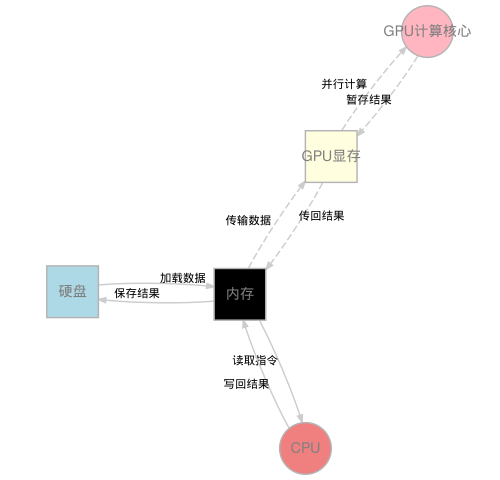
\includegraphics{imgs/hardware_flow.png}
\caption{\label{fig:hardware-flow}程序运行中的数据流动示意图}
\end{figure}

在统计分析的具体场景中,这种数据流转体现得更加明显。例如,当运行一个线性回归分析时:R解释器从硬盘读取脚本文件到内存;数据文件从硬盘加载到内存的数据框中;CPU执行lm()函数,在内存中进行矩阵运算;计算结果(系数、p值等)存储在内存中的模型对象里;最终结果被写入硬盘的报告文件。如果分析涉及大规模数据,可能会出现内存瓶颈,此时需要采用分批处理或流式处理策略,让数据在硬盘和内存间分块流动。

理解硬件组成和程序运行流程有助于统计分析人员优化工作流程。例如,知道CPU多核特性可以指导使用并行计算包(如parallel)来加速计算;了解GPU的并行能力可以指导选择适合GPU加速的算法;认识内存限制可以避免处理过大的数据集导致系统崩溃;理解硬盘性能差异可以优化数据存储策略。这种硬件意识是现代数据科学家必备的基础知识,它帮助研究者在技术约束下做出明智的决策,确保统计分析既高效又可靠。

\hypertarget{ux53d8ux91cfux4e0eux5e38ux91cf}{%
\subsubsection{变量与常量}\label{ux53d8ux91cfux4e0eux5e38ux91cf}}

\begin{Shaded}
\begin{Highlighting}[]
\CommentTok{\# 变量就像可擦写的白板,可以随时修改}
\NormalTok{score }\OtherTok{\textless{}{-}} \DecValTok{90}
\NormalTok{score }\OtherTok{\textless{}{-}} \DecValTok{95}  \CommentTok{\# 可以修改}

\CommentTok{\# 常量就像刻在石头上的字,一旦设定就不能改变}
\NormalTok{PI }\OtherTok{\textless{}{-}} \FloatTok{3.14159}
\CommentTok{\# PI \textless{}{-} 3.14  \# 不应该修改常量}
\end{Highlighting}
\end{Shaded}

\textbf{为什么重要}:变量和常量的区分体现了编程中的抽象思维和工程规范,是构建可维护、可复用代码的基础。在生态学数据分析中,这种区分尤为重要。变量就像生态学研究中的测量指标------它们会随着时间、空间或处理条件而变化,比如样地的温度读数、物种的个体数量、实验处理的效果值等。使用变量可以让代码适应不同的数据输入,实现分析的通用性和灵活性。而常量则代表那些在特定分析中保持不变的基础参数,比如圆周率π、重力加速度g、或者生态学中常用的转换系数(如生物量估算公式中的参数)。这些常量一旦设定就不应该被修改,因为它们代表了科学共识或物理规律。

从工程角度看,正确使用常量可以避免''魔法数字''问题------在代码中直接使用未经解释的数值,这不仅降低了代码的可读性,还增加了出错风险。比如,在计算森林碳储量时,如果直接将碳转换系数0.5写在计算公式中,其他研究者很难理解这个数字的含义,而且如果后续研究更新了这个系数,就需要在整个代码中搜索并修改所有出现0.5的地方。而如果将其定义为常量\texttt{CARBON\_CONVERSION\_FACTOR\ \textless{}-\ 0.5},代码就变得自文档化,修改也只需要在一个地方进行。

在生态学编程实践中,变量和常量的恰当使用还体现了对数据生命周期的理解。变量通常对应着分析过程中的中间结果或输入数据,它们的值会在分析流程中不断变化;而常量则对应着分析的基本假设和约束条件,它们定义了分析的边界和前提。这种区分有助于建立清晰的思维框架,让研究者能够更好地组织分析逻辑,确保代码的科学性和可复现性。更重要的是,在现代AI辅助编程环境中,明确的变量常量区分能够帮助LLM更好地理解代码意图,生成更符合生态学研究规范的解决方案。

\hypertarget{ux57faux672cux6570ux636eux7c7bux578b}{%
\subsubsection{基本数据类型}\label{ux57faux672cux6570ux636eux7c7bux578b}}

\begin{Shaded}
\begin{Highlighting}[]
\CommentTok{\# 数字类型}
\NormalTok{temperature }\OtherTok{\textless{}{-}} \FloatTok{25.5}
\NormalTok{count }\OtherTok{\textless{}{-}} \DecValTok{100}\DataTypeTok{L}

\CommentTok{\# 逻辑类型}
\NormalTok{is\_raining }\OtherTok{\textless{}{-}} \ConstantTok{TRUE}
\NormalTok{is\_sunny }\OtherTok{\textless{}{-}} \ConstantTok{FALSE}

\CommentTok{\# 字符类型}
\NormalTok{species\_name }\OtherTok{\textless{}{-}} \StringTok{"Quercus acutissima"}
\NormalTok{habitat }\OtherTok{\textless{}{-}} \StringTok{"deciduous forest"}

\CommentTok{\# 空值}
\NormalTok{missing\_data }\OtherTok{\textless{}{-}} \ConstantTok{NULL}
\end{Highlighting}
\end{Shaded}

\textbf{为什么重要}:数据类型的正确理解和使用是生态学数据分析的基石,它直接影响分析的准确性、效率和可解释性。在生态学研究中,不同类型的数据对应着不同的统计方法和生态学意义,混淆数据类型可能导致严重的科学错误。比如,物种名称是分类数据(字符型),应该使用频数统计和卡方检验;个体数量是计数数据(整数型),适合使用泊松回归或负二项回归;环境温度是连续数据(数值型),可以使用相关分析和回归模型;而存在/缺失数据(逻辑型)则需要使用二元响应模型。

从技术层面看,数据类型决定了可用的操作和函数。对数值型数据可以进行算术运算、统计检验和数学变换;对字符型数据可以进行字符串处理、模式匹配和分类汇总;对逻辑型数据可以进行逻辑运算和条件筛选。如果混淆了数据类型,比如试图对物种名称进行算术平均,或者对温度数据进行字符串拼接,不仅会产生无意义的结果,还可能导致程序错误。更重要的是,在生态学数据分析中,数据类型的选择往往反映了对生态现象的深刻理解------比如将连续的环境梯度离散化为分类变量时,需要基于生态学理论来确定分类边界。

在AI辅助编程时代,数据类型知识变得更加重要。当向LLM描述分析需求时,明确的数据类型说明能够帮助AI生成更准确的代码。比如,``分析温度对物种丰富度的影响''这个需求中,如果明确指出温度是连续变量,物种丰富度是计数变量,LLM就会推荐使用广义线性模型而不是普通的线性回归。此外,数据类型还关系到数据存储效率和计算性能------数值型数据比字符型数据占用更少内存,整数运算比浮点运算更快。在处理大规模的生态监测数据时,这种效率差异可能决定分析是否可行。因此,掌握数据类型不仅是编程技术问题,更是生态学研究者科学素养的体现。

\hypertarget{ux8fd0ux7b97ux7b26}{%
\subsubsection{运算符}\label{ux8fd0ux7b97ux7b26}}

\begin{Shaded}
\begin{Highlighting}[]
\CommentTok{\# 算术运算符}
\NormalTok{biomass }\OtherTok{\textless{}{-}}\NormalTok{ dbh}\SpecialCharTok{\^{}}\DecValTok{2} \SpecialCharTok{*}\NormalTok{ height }\SpecialCharTok{*} \FloatTok{0.6}  \CommentTok{\# 幂运算和乘法}

\CommentTok{\# 比较运算符}
\NormalTok{is\_large\_tree }\OtherTok{\textless{}{-}}\NormalTok{ dbh }\SpecialCharTok{\textgreater{}} \DecValTok{30}  \CommentTok{\# 大于比较}
\NormalTok{is\_same\_species }\OtherTok{\textless{}{-}}\NormalTok{ species1 }\SpecialCharTok{==}\NormalTok{ species2  }\CommentTok{\# 相等比较}

\CommentTok{\# 逻辑运算符}
\NormalTok{suitable\_habitat }\OtherTok{\textless{}{-}}\NormalTok{ (temperature }\SpecialCharTok{\textgreater{}} \DecValTok{15}\NormalTok{) }\SpecialCharTok{\&}\NormalTok{ (rainfall }\SpecialCharTok{\textgreater{}} \DecValTok{1000}\NormalTok{)  }\CommentTok{\# 与运算}
\NormalTok{rare\_species }\OtherTok{\textless{}{-}}\NormalTok{ (abundance }\SpecialCharTok{\textless{}} \DecValTok{10}\NormalTok{) }\SpecialCharTok{|}\NormalTok{ (distribution\_area }\SpecialCharTok{\textless{}} \DecValTok{100}\NormalTok{)  }\CommentTok{\# 或运算}

\CommentTok{\# 赋值运算符}
\NormalTok{species\_count }\OtherTok{\textless{}{-}} \FunctionTok{length}\NormalTok{(}\FunctionTok{unique}\NormalTok{(species\_list))  }\CommentTok{\# 常规赋值}
\end{Highlighting}
\end{Shaded}

\textbf{为什么重要}:运算符是编程语言中执行基本操作的核心元素,它们将简单的数据值组合成复杂的计算表达式。在生态学数据分析中,运算符的正确使用直接关系到分析结果的准确性和科学性。运算符可以分为几个主要类别:算术运算符(+、-、*、/、\^{})用于数值计算,如生物量估算、种群密度计算;比较运算符(\textgreater、\textless、==、!=)用于条件判断,如筛选特定大小的树木或特定温度范围的数据;逻辑运算符(\&、\textbar、!)用于组合多个条件,如同时满足温度和湿度要求的生态位分析。

运算符的优先级和结合性规则决定了复杂表达式的计算顺序,理解这些规则对于编写正确的代码至关重要。比如在表达式\texttt{a\ +\ b\ *\ c}中,乘法优先级高于加法,会先计算\texttt{b\ *\ c}再与\texttt{a}相加。如果不理解优先级,可能导致计算结果错误。在生态学建模中,这种精确性尤为重要------错误的运算符使用可能导致模型偏差或生态学意义的误解。

在AI协作环境中,明确的运算符使用能够显著提高与LLM的沟通效率。当向AI描述分析需求时,使用正确的运算符术语(如''使用逻辑与运算符组合温度和降水条件'')比模糊的描述(如''同时考虑温度和降水'')能生成更准确的代码。运算符还是连接数据与算法的桥梁,它们将原始生态数据转化为有意义的生态指标,是构建科学分析流程的基础构件。掌握运算符的使用不仅是一项编程技能,更是生态学研究者表达分析逻辑的重要工具。

\hypertarget{ux96c6ux5408ux6570ux636eux7c7bux578b}{%
\subsubsection{集合数据类型}\label{ux96c6ux5408ux6570ux636eux7c7bux578b}}

\begin{Shaded}
\begin{Highlighting}[]
\CommentTok{\# 向量 {-} 同类型元素的集合}
\NormalTok{temperatures }\OtherTok{\textless{}{-}} \FunctionTok{c}\NormalTok{(}\DecValTok{20}\NormalTok{, }\DecValTok{22}\NormalTok{, }\DecValTok{25}\NormalTok{, }\DecValTok{18}\NormalTok{, }\DecValTok{23}\NormalTok{)}
\NormalTok{species }\OtherTok{\textless{}{-}} \FunctionTok{c}\NormalTok{(}\StringTok{"Oak"}\NormalTok{, }\StringTok{"Pine"}\NormalTok{, }\StringTok{"Maple"}\NormalTok{, }\StringTok{"Birch"}\NormalTok{)}

\CommentTok{\# 列表 {-} 可以包含不同类型的元素}
\NormalTok{forest\_data }\OtherTok{\textless{}{-}} \FunctionTok{list}\NormalTok{(}
  \AttributeTok{name =} \StringTok{"Tianmu Mountain Forest"}\NormalTok{,}
  \AttributeTok{area =} \DecValTok{428}\NormalTok{,}
  \AttributeTok{dominant\_species =} \FunctionTok{c}\NormalTok{(}\StringTok{"Cyclobalanopsis"}\NormalTok{, }\StringTok{"Castanopsis"}\NormalTok{),}
  \AttributeTok{elevation\_range =} \FunctionTok{c}\NormalTok{(}\DecValTok{300}\NormalTok{, }\DecValTok{1500}\NormalTok{)}
\NormalTok{)}

\CommentTok{\# 数据框 {-} 表格形式的数据}
\NormalTok{forest\_df }\OtherTok{\textless{}{-}} \FunctionTok{data.frame}\NormalTok{(}
  \AttributeTok{plot\_id =} \DecValTok{1}\SpecialCharTok{:}\DecValTok{5}\NormalTok{,}
  \AttributeTok{species =} \FunctionTok{c}\NormalTok{(}\StringTok{"Quercus"}\NormalTok{, }\StringTok{"Pinus"}\NormalTok{, }\StringTok{"Acer"}\NormalTok{, }\StringTok{"Betula"}\NormalTok{, }\StringTok{"Fagus"}\NormalTok{),}
  \AttributeTok{dbh =} \FunctionTok{c}\NormalTok{(}\FloatTok{25.3}\NormalTok{, }\FloatTok{18.7}\NormalTok{, }\FloatTok{12.4}\NormalTok{, }\FloatTok{15.8}\NormalTok{, }\FloatTok{22.1}\NormalTok{),}
  \AttributeTok{height =} \FunctionTok{c}\NormalTok{(}\FloatTok{18.2}\NormalTok{, }\FloatTok{15.6}\NormalTok{, }\FloatTok{10.3}\NormalTok{, }\FloatTok{12.7}\NormalTok{, }\FloatTok{16.9}\NormalTok{)}
\NormalTok{)}
\end{Highlighting}
\end{Shaded}

\textbf{为什么重要}:集合数据类型的正确选择是生态学数据分析效率和质量的关键,它体现了对数据结构复杂性和分析需求的深刻理解。与基本数据类型(如数值、字符、逻辑值)处理单个数据元素不同,集合数据类型用于组织和存储多个相关数据,每种类型都有其独特的结构特性和适用场景。在生态学研究中,这种区分尤为重要------向量适合存储同类型的观测序列(如连续的温度读数),列表能够容纳复杂的嵌套结构(如包含样地信息、物种组成、环境因子的综合数据),而数据框则专门为表格型数据设计(如样地调查表)。

基本数据类型与集合数据类型的根本区别在于组织层次和操作粒度。基本数据类型关注单个数据点的属性和操作,比如数值的算术运算、字符的字符串处理;而集合数据类型关注数据之间的组织关系和整体操作,比如向量的元素索引、列表的嵌套访问、数据框的行列筛选。这种区别决定了它们的使用场景:当需要处理单一类型的序列数据时,向量提供了高效的内存存储和向量化运算;当数据结构复杂且异构时,列表的灵活性允许存储不同类型的数据对象;当数据呈现表格形式且需要同时处理多个变量时,数据框的结构化存储便于统计分析。

在生态学数据分析实践中,正确的集合类型选择直接影响分析效率和结果质量。比如,使用向量存储物种多样性指数序列可以实现快速的统计计算和可视化;使用列表组织不同样地的监测数据便于批量处理和比较分析;使用数据框管理样地调查表则可以直接应用各种统计函数和机器学习算法。更重要的是,集合数据类型的选择反映了对生态数据本质的理解------是时间序列、空间分布还是多变量关系?这种理解有助于设计更合理的分析流程,确保统计方法的适用性和结果的科学性。在AI协作环境中,明确的集合类型说明能够帮助LLM生成更符合生态学数据分析规范的代码,提高协作效率。

\hypertarget{ux5206ux652fux4e0eux5faaux73af}{%
\subsubsection{分支与循环}\label{ux5206ux652fux4e0eux5faaux73af}}

\begin{Shaded}
\begin{Highlighting}[]
\CommentTok{\# 条件判断 {-} 根据条件选择不同路径}
\NormalTok{classify\_tree\_size }\OtherTok{\textless{}{-}} \ControlFlowTok{function}\NormalTok{(dbh) \{}
  \ControlFlowTok{if}\NormalTok{ (dbh }\SpecialCharTok{\textless{}} \DecValTok{10}\NormalTok{) \{}
    \FunctionTok{return}\NormalTok{(}\StringTok{"sapling"}\NormalTok{)}
\NormalTok{  \} }\ControlFlowTok{else} \ControlFlowTok{if}\NormalTok{ (dbh }\SpecialCharTok{\textless{}} \DecValTok{30}\NormalTok{) \{}
    \FunctionTok{return}\NormalTok{(}\StringTok{"medium tree"}\NormalTok{)}
\NormalTok{  \} }\ControlFlowTok{else}\NormalTok{ \{}
    \FunctionTok{return}\NormalTok{(}\StringTok{"large tree"}\NormalTok{)}
\NormalTok{  \}}
\NormalTok{\}}

\CommentTok{\# 循环 {-} 重复执行操作}
\CommentTok{\# 计算每个样地的平均胸径}
\NormalTok{plot\_dbh }\OtherTok{\textless{}{-}} \FunctionTok{c}\NormalTok{(}\FloatTok{15.3}\NormalTok{, }\FloatTok{22.7}\NormalTok{, }\FloatTok{18.4}\NormalTok{, }\FloatTok{25.1}\NormalTok{, }\FloatTok{12.9}\NormalTok{)}
\NormalTok{average\_dbh }\OtherTok{\textless{}{-}} \FunctionTok{numeric}\NormalTok{(}\FunctionTok{length}\NormalTok{(plot\_dbh))}

\ControlFlowTok{for}\NormalTok{ (i }\ControlFlowTok{in} \DecValTok{1}\SpecialCharTok{:}\FunctionTok{length}\NormalTok{(plot\_dbh)) \{}
\NormalTok{  average\_dbh[i] }\OtherTok{\textless{}{-}} \FunctionTok{mean}\NormalTok{(plot\_dbh[}\DecValTok{1}\SpecialCharTok{:}\NormalTok{i])}
\NormalTok{\}}

\CommentTok{\# 更R风格的方式 {-} 使用向量化操作}
\NormalTok{average\_dbh }\OtherTok{\textless{}{-}} \FunctionTok{cumsum}\NormalTok{(plot\_dbh) }\SpecialCharTok{/} \DecValTok{1}\SpecialCharTok{:}\FunctionTok{length}\NormalTok{(plot\_dbh)}
\end{Highlighting}
\end{Shaded}

\textbf{为什么重要}:分支与循环是构建复杂生态学数据分析逻辑的核心工具,它们将静态的数据处理转化为动态的、智能的分析流程。在生态学研究中,自然系统的复杂性和不确定性要求分析程序能够根据数据特征自动调整处理策略,这正是分支结构的价值所在。比如,在分析物种分布数据时,可能需要根据数据质量(完整性、准确性)选择不同的预处理方法;在处理环境梯度数据时,需要根据变量类型(连续型、分类型)应用不同的统计模型。这种条件判断能力使得分析程序能够适应真实世界的复杂性,而不是僵化地套用固定流程。

循环结构则解决了生态学数据分析中的规模化问题。生态学研究往往涉及大量的重复性操作------对数百个样地的数据执行相同的计算,对数十个环境变量进行相同的统计分析,对多年的监测数据进行相同的时间序列分析。手动重复这些操作不仅效率低下,还容易出错。循环结构通过自动化这些重复任务,确保了分析的一致性和可复现性。更重要的是,在R语言中,向量化操作往往比显式循环更高效,这体现了对计算效率的深入理解。

分支与循环的组合使用能够构建出真正智能的数据分析系统。比如,一个完整的生态数据分析流程可能包含:首先使用循环遍历所有样地,对每个样地使用分支结构检查数据质量,然后根据质量等级选择不同的清洗策略,接着使用嵌套循环分析不同时间尺度的变化模式,最后根据统计显著性自动生成报告结论。这种复杂的逻辑结构正是现代生态学研究所需的------它能够处理大规模、多维度、异质性的生态数据,产生科学可靠的结论。在AI协作时代,理解这些控制结构有助于更好地指导LLM生成符合生态学分析逻辑的代码,而不是简单的脚本堆积。

\textbf{向量化操作的重要性}:在R语言中,向量化操作代表了更高级的编程思维,它通过将操作应用于整个数据向量而非单个元素,极大地简化了数据分析代码。对于生态学研究者而言,向量化不仅意味着代码简洁性的提升------比如用\texttt{mean(temperature)}替代繁琐的循环计算,更重要的是它体现了对数据整体性的理解。在处理生态监测数据时,向量化操作允许研究者一次性对整个时间序列或空间网格进行分析,而不是逐点处理,这大大提高了代码的可读性和可维护性。

从性能角度看,向量化操作通常比显式循环运行更快,因为R的内部优化能够利用底层C/Fortran代码的高效实现。这种性能优势在R、Python等解释型语言中尤为明显,因为这些语言中的循环通常较慢。相比之下,在C++等编译型语言中,循环本身已经高度优化,向量化的性能优势相对较小,但向量化思维仍然有助于简化代码语法。在处理大规模的生态数据集(如遥感影像、长期监测记录)时,这种速度优势可能决定分析是否可行。然而,向量化操作也有其局限性:它要求数据具有相同的结构和类型,对于复杂的分支逻辑或条件处理可能不够灵活。此外,过度向量化可能降低代码的可调试性,因为错误可能隐藏在复杂的向量运算中。另一个重要缺陷是内存消耗问题:向量化操作通常需要将整个数据集加载到内存中进行批量处理,对于超大规模的生态数据集(如高分辨率遥感影像、全基因组序列),这可能超出计算机的内存容量,导致程序崩溃。相比之下,循环处理可以逐块读取数据,减少内存压力。因此,生态学研究者需要在向量化的简洁高效与循环的灵活可控之间找到平衡,根据具体分析需求选择最合适的编程范式。

\hypertarget{ux8868ux8fbeux5f0fux4e0eux8bedux53e5}{%
\subsubsection{表达式与语句}\label{ux8868ux8fbeux5f0fux4e0eux8bedux53e5}}

\begin{Shaded}
\begin{Highlighting}[]
\CommentTok{\# 表达式 {-} 产生值的代码片段}
\NormalTok{total\_trees }\OtherTok{\textless{}{-}} \DecValTok{100} \SpecialCharTok{+} \DecValTok{50}  \CommentTok{\# 表达式,产生值150}
\NormalTok{mean\_dbh }\OtherTok{\textless{}{-}} \FunctionTok{mean}\NormalTok{(}\FunctionTok{c}\NormalTok{(}\DecValTok{25}\NormalTok{, }\DecValTok{30}\NormalTok{, }\DecValTok{35}\NormalTok{))  }\CommentTok{\# 表达式,产生平均值}

\CommentTok{\# 语句 {-} 执行动作的代码单元}
\ControlFlowTok{if}\NormalTok{ (temperature }\SpecialCharTok{\textgreater{}} \DecValTok{25}\NormalTok{) \{}
  \FunctionTok{cat}\NormalTok{(}\StringTok{"温度过高,需要调整实验条件}\SpecialCharTok{\textbackslash{}n}\StringTok{"}\NormalTok{)  }\CommentTok{\# 语句}
\NormalTok{\}}
\ControlFlowTok{for}\NormalTok{ (plot }\ControlFlowTok{in}\NormalTok{ plots) \{}
  \FunctionTok{analyze\_plot}\NormalTok{(plot)  }\CommentTok{\# 语句}
\NormalTok{\}}
\end{Highlighting}
\end{Shaded}

\textbf{为什么重要}:表达式与语句的区分体现了编程中的两种基本思维模式------计算思维和流程控制思维。表达式(Expression)是能够产生值的代码片段,它们关注''计算什么'',通过运算符和函数调用来完成具体的数值计算或逻辑判断。比如\texttt{dbh\^{}2\ *\ height\ *\ 0.6}是一个表达式,它计算树木的生物量;\texttt{temperature\ \textgreater{}\ 25}也是一个表达式,它产生逻辑值TRUE或FALSE。表达式可以嵌套组合,形成复杂的计算逻辑,但最终都会归结为一个具体的值。

语句(Statement)则是执行动作的代码单元,它们关注''做什么'',控制程序的执行流程。语句不产生值(或者产生的值不是其主要目的),而是完成特定的操作任务。前面提到的分支(if-else)和循环(for/while)都是典型的语句类型------分支语句根据条件选择不同的执行路径,循环语句重复执行特定的代码块。其他常见的语句还包括赋值语句(\texttt{x\ \textless{}-\ 10})、函数调用语句等。

这种区分在生态学数据分析中尤为重要:表达式用于构建统计模型和计算生态指标,如多样性指数计算、回归分析等;语句则用于控制分析流程,如根据数据质量选择不同的预处理方法,或者对多个样地执行相同的分析操作。理解这种区别有助于设计更清晰的分析架构,也便于与LLM有效协作------明确告诉AI需要计算什么(表达式)和需要执行什么操作(语句)。

\hypertarget{ux51fdux6570ux8fc7ux7a0b}{%
\subsubsection{函数/过程}\label{ux51fdux6570ux8fc7ux7a0b}}

\begin{Shaded}
\begin{Highlighting}[]
\CommentTok{\# 定义计算物种多样性的函数}
\NormalTok{calculate\_diversity }\OtherTok{\textless{}{-}} \ControlFlowTok{function}\NormalTok{(species\_list) \{}
\NormalTok{  species\_counts }\OtherTok{\textless{}{-}} \FunctionTok{table}\NormalTok{(species\_list)}
\NormalTok{  proportions }\OtherTok{\textless{}{-}}\NormalTok{ species\_counts }\SpecialCharTok{/} \FunctionTok{sum}\NormalTok{(species\_counts)}
\NormalTok{  shannon }\OtherTok{\textless{}{-}} \SpecialCharTok{{-}}\FunctionTok{sum}\NormalTok{(proportions }\SpecialCharTok{*} \FunctionTok{log}\NormalTok{(proportions))}
  \FunctionTok{return}\NormalTok{(shannon)}
\NormalTok{\}}

\CommentTok{\# 定义数据清洗函数}
\NormalTok{clean\_forest\_data }\OtherTok{\textless{}{-}} \ControlFlowTok{function}\NormalTok{(raw\_data) \{}
\NormalTok{  cleaned }\OtherTok{\textless{}{-}}\NormalTok{ raw\_data }\SpecialCharTok{\%\textgreater{}\%}
    \FunctionTok{filter}\NormalTok{(}\SpecialCharTok{!}\FunctionTok{is.na}\NormalTok{(dbh) }\SpecialCharTok{\&}\NormalTok{ dbh }\SpecialCharTok{\textgreater{}} \DecValTok{0}\NormalTok{) }\SpecialCharTok{\%\textgreater{}\%}
    \FunctionTok{mutate}\NormalTok{(}\AttributeTok{species =} \FunctionTok{str\_trim}\NormalTok{(}\FunctionTok{tolower}\NormalTok{(species)))}
  \FunctionTok{return}\NormalTok{(cleaned)}
\NormalTok{\}}

\CommentTok{\# 使用函数}
\NormalTok{sample\_species }\OtherTok{\textless{}{-}} \FunctionTok{c}\NormalTok{(}\StringTok{"Oak"}\NormalTok{, }\StringTok{"Pine"}\NormalTok{, }\StringTok{"Oak"}\NormalTok{, }\StringTok{"Maple"}\NormalTok{)}
\NormalTok{diversity\_index }\OtherTok{\textless{}{-}} \FunctionTok{calculate\_diversity}\NormalTok{(sample\_species)}
\NormalTok{cleaned\_data }\OtherTok{\textless{}{-}} \FunctionTok{clean\_forest\_data}\NormalTok{(raw\_forest\_data)}
\end{Highlighting}
\end{Shaded}

\textbf{为什么重要}:函数是编程中的抽象工具,它将复杂的操作封装成可重用的模块,体现了''一次编写,多次使用''的工程原则。在生态学数据分析中,函数的使用具有多重价值:首先是代码复用性------相同的分析逻辑可以在不同项目、不同数据集中重复使用,避免重复劳动。比如,一个计算Shannon多样性指数的函数可以在多个森林调查项目中重复使用,大大提高了分析效率。其次是可维护性------当分析逻辑需要修改时,只需修改函数定义,所有调用该函数的地方都会自动更新。例如,如果需要改进多样性指数的计算方法,只需修改\texttt{calculate\_diversity}函数,而不需要在每个使用该计算的地方逐一修改。再次是模块化设计------通过将复杂分析流程分解为多个函数,使代码结构更清晰,便于理解和调试。在生态学研究中,一个完整的分析流程可能包含数据读取、清洗、多样性计算、统计检验、可视化等多个步骤,每个步骤都可以封装为独立的函数,使整体分析逻辑更加清晰。

从工程角度看,函数还促进了代码的标准化和规范化。在团队协作的生态学研究项目中,统一的函数接口可以确保不同研究者使用相同的分析方法,提高结果的可比性和可复现性。例如,定义标准的\texttt{clean\_forest\_data}函数可以确保所有参与者在数据清洗阶段采用相同的质量控制标准。

在AI协作环境中,函数思维变得更加重要。当向LLM描述分析需求时,明确的函数化架构能够帮助AI更好地理解分析逻辑,生成更模块化、可维护的代码。LLM可以根据函数化的需求描述,分别生成数据读取、处理、分析、可视化等各个模块的代码,而不是生成一个冗长复杂的单一脚本。这种模块化的代码结构不仅便于人类理解,也便于后续的调试和优化。更重要的是,函数化的思维有助于建立清晰的测试框架------每个函数都可以独立测试,确保其功能的正确性,从而提高整个分析流程的可靠性。在生态学数据分析的复杂环境中,这种函数化的设计思维是确保分析质量、提高协作效率的关键保障。

\hypertarget{ux4f5cux7528ux57df}{%
\subsubsection{作用域}\label{ux4f5cux7528ux57df}}

\begin{Shaded}
\begin{Highlighting}[]
\CommentTok{\# 全局变量}
\NormalTok{global\_species\_count }\OtherTok{\textless{}{-}} \DecValTok{0}

\NormalTok{analyze\_forest }\OtherTok{\textless{}{-}} \ControlFlowTok{function}\NormalTok{(plot\_data) \{}
  \CommentTok{\# 局部变量 {-} 只在函数内部可见}
\NormalTok{  local\_species }\OtherTok{\textless{}{-}} \FunctionTok{unique}\NormalTok{(plot\_data}\SpecialCharTok{$}\NormalTok{species)}
\NormalTok{  local\_count }\OtherTok{\textless{}{-}} \FunctionTok{length}\NormalTok{(local\_species)}

  \CommentTok{\# 可以访问全局变量}
\NormalTok{  global\_species\_count }\OtherTok{\textless{}\textless{}{-}}\NormalTok{ global\_species\_count }\SpecialCharTok{+}\NormalTok{ local\_count}

  \FunctionTok{return}\NormalTok{(local\_count)}
\NormalTok{\}}

\CommentTok{\# 在函数外部无法访问局部变量}
\CommentTok{\# print(local\_species)  \# 会报错}

\CommentTok{\# 但可以访问全局变量}
\FunctionTok{print}\NormalTok{(global\_species\_count)}
\end{Highlighting}
\end{Shaded}

\textbf{为什么重要}:作用域规则定义了变量的可见范围,是构建复杂、安全程序的基础机制。在生态学数据分析中,正确理解作用域具有多重重要意义:首先,作用域机制有效避免了命名冲突------不同的函数或模块可以使用相同的变量名而不会相互干扰。例如,在分析多个样地数据时,每个样地的分析函数都可以使用\texttt{species\_count}作为局部变量,而不会影响其他样地的计算结果。这种隔离性大大简化了变量命名,降低了代码复杂度。

其次,作用域提供了精细的数据访问控制能力。在生态学研究中,某些敏感数据(如原始调查记录、物种分布坐标等)需要限制访问范围,防止意外修改或泄露。通过将敏感数据封装在特定作用域内,可以确保只有授权的函数能够访问和修改这些数据,提高了代码的安全性。

第三,作用域规则优化了内存管理效率。局部变量在函数执行结束时自动释放,避免了内存泄漏问题。在处理大规模的生态监测数据时,这种自动内存管理机制尤为重要,可以防止因变量积累导致的内存耗尽问题。例如,在循环处理多个年份的监测数据时,每次迭代的临时变量都会在迭代结束后自动清理,确保内存使用的高效性。

从软件工程角度看,作用域概念体现了信息隐藏原则,是构建模块化、健壮分析系统的关键。通过将内部实现细节隐藏在局部作用域中,只暴露必要的接口,可以降低模块间的耦合度,提高代码的可维护性和可扩展性。在团队协作的生态学研究项目中,明确的作用域规则可以防止意外的变量修改,确保不同开发者编写的代码能够安全地集成在一起。特别是在AI协作环境中,清晰的作用域设计有助于LLM生成更结构化的代码,避免全局变量污染和意外的副作用,从而提高生成代码的质量和可靠性。

\hypertarget{ux9519ux8befux4e0eux5f02ux5e38ux5904ux7406}{%
\subsubsection{错误与异常处理}\label{ux9519ux8befux4e0eux5f02ux5e38ux5904ux7406}}

\begin{Shaded}
\begin{Highlighting}[]
\CommentTok{\# 基本的错误处理}
\NormalTok{safe\_division }\OtherTok{\textless{}{-}} \ControlFlowTok{function}\NormalTok{(numerator, denominator) \{}
  \ControlFlowTok{if}\NormalTok{ (denominator }\SpecialCharTok{==} \DecValTok{0}\NormalTok{) \{}
    \FunctionTok{stop}\NormalTok{(}\StringTok{"分母不能为零"}\NormalTok{)}
\NormalTok{  \}}
  \FunctionTok{return}\NormalTok{(numerator }\SpecialCharTok{/}\NormalTok{ denominator)}
\NormalTok{\}}

\CommentTok{\# 使用tryCatch进行异常处理}
\NormalTok{analyze\_with\_safety }\OtherTok{\textless{}{-}} \ControlFlowTok{function}\NormalTok{(data\_file) \{}
\NormalTok{  result }\OtherTok{\textless{}{-}} \FunctionTok{tryCatch}\NormalTok{(\{}
    \CommentTok{\# 尝试执行可能出错的操作}
\NormalTok{    data }\OtherTok{\textless{}{-}} \FunctionTok{read.csv}\NormalTok{(data\_file)}
\NormalTok{    diversity }\OtherTok{\textless{}{-}} \FunctionTok{calculate\_diversity}\NormalTok{(data}\SpecialCharTok{$}\NormalTok{species)}
    \FunctionTok{return}\NormalTok{(diversity)}
\NormalTok{  \}, }\AttributeTok{error =} \ControlFlowTok{function}\NormalTok{(e) \{}
    \CommentTok{\# 错误处理}
    \FunctionTok{cat}\NormalTok{(}\StringTok{"分析失败:"}\NormalTok{, e}\SpecialCharTok{$}\NormalTok{message, }\StringTok{"}\SpecialCharTok{\textbackslash{}n}\StringTok{"}\NormalTok{)}
    \FunctionTok{return}\NormalTok{(}\ConstantTok{NA}\NormalTok{)}
\NormalTok{  \}, }\AttributeTok{warning =} \ControlFlowTok{function}\NormalTok{(w) \{}
    \CommentTok{\# 警告处理}
    \FunctionTok{cat}\NormalTok{(}\StringTok{"警告:"}\NormalTok{, w}\SpecialCharTok{$}\NormalTok{message, }\StringTok{"}\SpecialCharTok{\textbackslash{}n}\StringTok{"}\NormalTok{)}
    \FunctionTok{return}\NormalTok{(}\FunctionTok{calculate\_diversity}\NormalTok{(data}\SpecialCharTok{$}\NormalTok{species))  }\CommentTok{\# 继续执行}
\NormalTok{  \})}

  \FunctionTok{return}\NormalTok{(result)}
\NormalTok{\}}

\CommentTok{\# 使用示例}
\NormalTok{try\_result }\OtherTok{\textless{}{-}} \FunctionTok{analyze\_with\_safety}\NormalTok{(}\StringTok{"missing\_file.csv"}\NormalTok{)}
\end{Highlighting}
\end{Shaded}

\textbf{为什么重要}:错误与异常处理是构建健壮分析系统的关键机制,它确保程序在遇到意外情况时能够优雅地处理而不是崩溃。在生态学数据分析中,异常处理尤为重要,因为野外数据往往存在各种质量问题------文件缺失、格式错误、数据异常等。生态学研究的数据来源多样,包括野外调查记录、传感器监测、遥感影像等,这些数据在收集、传输和处理过程中容易出现各种问题。例如,野外调查可能因天气原因中断导致数据不完整,传感器可能因故障产生异常值,不同数据源可能使用不同的格式标准。

通过合理的错误处理,可以显著提高程序的稳定性。在复杂的生态数据分析流程中,一个环节的错误不应该导致整个分析流程的崩溃。例如,当处理多个样地的调查数据时,如果某个样地文件损坏或格式错误,异常处理机制可以捕获这个错误,记录问题并继续处理其他样地,而不是让整个批处理作业失败。这种容错能力对于长期生态监测项目尤为重要,因为数据收集往往跨越数年甚至数十年,期间难免会出现各种技术问题。

异常处理还能提供友好的用户体验。相比于直接显示晦涩的技术错误信息,精心设计的异常处理可以给出清晰、有指导意义的提示。例如,当数据文件缺失时,可以提示用户检查文件路径或提供替代数据源;当数据格式错误时,可以指出具体的问题所在并建议修正方法。这种用户友好的错误处理不仅提高了工具的易用性,也降低了非技术用户的使用门槛。

在自动化流程中,异常处理是确保连续运行的关键。生态学研究经常需要处理大规模数据集,如多年的气候监测数据或大范围的遥感影像。在这些场景下,手动干预每个错误是不现实的。通过异常处理机制,程序可以自动跳过问题数据、记录错误日志、尝试替代方案,确保分析流程能够持续运行。例如,在批量计算物种多样性指数时,如果某个样地的数据质量不合格,程序可以自动标记该样地并继续处理其他样地。

在AI生成代码的背景下,添加适当的错误处理是确保代码质量的重要环节。LLM生成的代码往往侧重于功能实现,可能忽略边界情况和异常处理。作为代码审查者,需要特别关注错误处理机制的完整性,确保生成的代码能够应对各种意外情况。同时,在向LLM描述需求时,明确要求包含完善的错误处理逻辑,可以显著提高生成代码的健壮性和实用性。

\hypertarget{ux6a21ux5757ux5316ux4e0eux5305ux7ba1ux7406}{%
\subsubsection{模块化与包管理}\label{ux6a21ux5757ux5316ux4e0eux5305ux7ba1ux7406}}

\begin{Shaded}
\begin{Highlighting}[]
\CommentTok{\# 模块化代码组织}
\CommentTok{\# data\_processing.R {-} 数据处理模块}
\NormalTok{clean\_data }\OtherTok{\textless{}{-}} \ControlFlowTok{function}\NormalTok{(raw\_data) \{ }\SpecialCharTok{/}\ErrorTok{*}\NormalTok{ 数据清洗逻辑 }\SpecialCharTok{*}\ErrorTok{/}\NormalTok{ \}}
\NormalTok{normalize\_data }\OtherTok{\textless{}{-}} \ControlFlowTok{function}\NormalTok{(data) \{ }\SpecialCharTok{/}\ErrorTok{*}\NormalTok{ 数据标准化逻辑 }\SpecialCharTok{*}\ErrorTok{/}\NormalTok{ \}}

\CommentTok{\# analysis.R {-} 分析模块}
\NormalTok{calculate\_diversity }\OtherTok{\textless{}{-}} \ControlFlowTok{function}\NormalTok{(species) \{ }\SpecialCharTok{/}\ErrorTok{*}\NormalTok{ 多样性计算 }\SpecialCharTok{*}\ErrorTok{/}\NormalTok{ \}}
\NormalTok{perform\_stat\_test }\OtherTok{\textless{}{-}} \ControlFlowTok{function}\NormalTok{(data) \{ }\SpecialCharTok{/}\ErrorTok{*}\NormalTok{ 统计检验 }\SpecialCharTok{*}\ErrorTok{/}\NormalTok{ \}}

\CommentTok{\# visualization.R {-} 可视化模块}
\NormalTok{create\_plots }\OtherTok{\textless{}{-}} \ControlFlowTok{function}\NormalTok{(results) \{ }\SpecialCharTok{/}\ErrorTok{*}\NormalTok{ 图表生成 }\SpecialCharTok{*}\ErrorTok{/}\NormalTok{ \}}

\CommentTok{\# 主程序 {-} 协调各个模块}
\FunctionTok{source}\NormalTok{(}\StringTok{"data\_processing.R"}\NormalTok{)}
\FunctionTok{source}\NormalTok{(}\StringTok{"analysis.R"}\NormalTok{)}
\FunctionTok{source}\NormalTok{(}\StringTok{"visualization.R"}\NormalTok{)}

\CommentTok{\# 使用包管理}
\FunctionTok{library}\NormalTok{(dplyr)    }\CommentTok{\# 数据处理}
\FunctionTok{library}\NormalTok{(ggplot2)  }\CommentTok{\# 数据可视化}
\FunctionTok{library}\NormalTok{(vegan)    }\CommentTok{\# 生态学分析}
\end{Highlighting}
\end{Shaded}

\textbf{为什么重要}:模块化与包管理是构建可维护、可扩展分析系统的核心实践。模块化将复杂的分析流程分解为职责单一、接口清晰的代码单元,这种分解思维在生态学数据分析中具有深远的意义。从技术层面看,模块化显著提高了代码的可读性、可测试性和可维护性。一个典型的生态数据分析项目可能包含数据收集、清洗、统计分析、可视化等多个环节,将这些环节模块化后,每个模块都可以独立开发、测试和优化。例如,数据清洗模块可以专注于处理缺失值和异常值,统计分析模块可以专注于算法实现,可视化模块可以专注于图表设计。这种职责分离使得代码结构更加清晰,便于理解和维护。

包管理则代表了现代编程的协作智慧,它充分利用社区资源,避免重复造轮子。在生态学领域,R语言的包生态系统尤为丰富,提供了大量专业工具。vegan包专门用于生态学多样性分析,spatstat包提供了空间点模式分析的完整解决方案,sp包处理空间数据,lme4包实现混合效应模型等。这些经过社区验证的包不仅提供了可靠的功能实现,还包含了最佳实践和标准方法。

特别值得一提的是spatstat包,它本身就是模块化设计的典范。spatstat将复杂的空间统计分析功能分解为多个子包:spatstat.core处理核心的点模式分析功能,spatstat.geom提供几何操作,spatstat.model实现统计模型,spatstat.explore支持探索性分析等。这种精细的模块化设计让用户可以根据具体需求选择性地加载所需功能,避免不必要的内存开销,同时也便于功能的独立开发和维护。

使用这些专业包,研究者可以快速构建复杂的分析流程,而不需要从零开始实现基础功能。例如,计算物种多样性指数时,直接使用vegan包的\texttt{diversity()}函数,既保证了计算准确性,又节省了开发时间。在进行空间点模式分析时,使用spatstat包可以轻松实现Ripley's K函数、对相关函数等复杂的空间统计方法。

在团队协作的生态学研究项目中,模块化架构特别重要。不同研究者可以负责不同模块的开发,如生态学家专注于分析逻辑的实现,程序员专注于技术架构的优化。清晰的模块接口确保了各个部分能够无缝集成,避免了因代码耦合度过高导致的协作困难。同时,模块化支持代码的渐进式改进------可以单独优化某个模块而不影响其他部分,这种灵活性对于长期的研究项目尤为重要。

包管理还促进了分析方法的标准化和可复现性。当整个研究领域都使用相同的分析包时,不同研究的结果具有更好的可比性。例如,如果所有森林生态学研究都使用vegan包计算多样性指数,那么不同研究的结果就可以进行有意义的比较和整合。这种标准化对于生态学知识的积累和科学共识的形成至关重要。

在AI时代,模块化思维变得更加重要。当向LLM描述分析需求时,明确的模块化架构能够帮助AI生成更结构化的代码。LLM可以根据模块化的需求描述,分别生成数据读取、处理、分析、可视化等各个模块的代码,而不是生成一个冗长复杂的单一脚本。这种模块化的代码不仅便于人类理解,也便于后续的调试、优化和扩展。更重要的是,模块化思维有助于建立清晰的测试框架------每个模块都可以独立测试,确保其功能的正确性,从而提高整个分析流程的可靠性。

\hypertarget{ux9762ux5411ux5bf9ux8c61ux57faux7840}{%
\subsubsection{面向对象基础}\label{ux9762ux5411ux5bf9ux8c61ux57faux7840}}

\begin{Shaded}
\begin{Highlighting}[]
\CommentTok{\# 简单的面向对象示例 {-} 使用S3系统}
\CommentTok{\# 定义物种类}
\NormalTok{species }\OtherTok{\textless{}{-}} \ControlFlowTok{function}\NormalTok{(name, abundance, habitat) \{}
  \FunctionTok{structure}\NormalTok{(}\FunctionTok{list}\NormalTok{(}
    \AttributeTok{name =}\NormalTok{ name,}
    \AttributeTok{abundance =}\NormalTok{ abundance,}
    \AttributeTok{habitat =}\NormalTok{ habitat}
\NormalTok{  ), }\AttributeTok{class =} \StringTok{"species"}\NormalTok{)}
\NormalTok{\}}

\CommentTok{\# 定义方法}
\NormalTok{print.species }\OtherTok{\textless{}{-}} \ControlFlowTok{function}\NormalTok{(x) \{}
  \FunctionTok{cat}\NormalTok{(}\StringTok{"物种:"}\NormalTok{, x}\SpecialCharTok{$}\NormalTok{name, }\StringTok{"}\SpecialCharTok{\textbackslash{}n}\StringTok{"}\NormalTok{)}
  \FunctionTok{cat}\NormalTok{(}\StringTok{"多度:"}\NormalTok{, x}\SpecialCharTok{$}\NormalTok{abundance, }\StringTok{"}\SpecialCharTok{\textbackslash{}n}\StringTok{"}\NormalTok{)}
  \FunctionTok{cat}\NormalTok{(}\StringTok{"生境:"}\NormalTok{, x}\SpecialCharTok{$}\NormalTok{habitat, }\StringTok{"}\SpecialCharTok{\textbackslash{}n}\StringTok{"}\NormalTok{)}
\NormalTok{\}}

\CommentTok{\# 使用示例}
\NormalTok{oak }\OtherTok{\textless{}{-}} \FunctionTok{species}\NormalTok{(}\StringTok{"Quercus"}\NormalTok{, }\DecValTok{150}\NormalTok{, }\StringTok{"deciduous\_forest"}\NormalTok{)}
\FunctionTok{print}\NormalTok{(oak)}

\CommentTok{\# 更现代的R6系统示例}
\FunctionTok{library}\NormalTok{(R6)}

\NormalTok{ForestPlot }\OtherTok{\textless{}{-}} \FunctionTok{R6Class}\NormalTok{(}\StringTok{"ForestPlot"}\NormalTok{,}
  \AttributeTok{public =} \FunctionTok{list}\NormalTok{(}
    \AttributeTok{plot\_id =} \ConstantTok{NULL}\NormalTok{,}
    \AttributeTok{species\_list =} \ConstantTok{NULL}\NormalTok{,}

    \AttributeTok{initialize =} \ControlFlowTok{function}\NormalTok{(plot\_id, species\_list) \{}
\NormalTok{      self}\SpecialCharTok{$}\NormalTok{plot\_id }\OtherTok{\textless{}{-}}\NormalTok{ plot\_id}
\NormalTok{      self}\SpecialCharTok{$}\NormalTok{species\_list }\OtherTok{\textless{}{-}}\NormalTok{ species\_list}
\NormalTok{    \},}

    \AttributeTok{calculate\_diversity =} \ControlFlowTok{function}\NormalTok{() \{}
      \FunctionTok{table}\NormalTok{(self}\SpecialCharTok{$}\NormalTok{species\_list) }\SpecialCharTok{\%\textgreater{}\%} \FunctionTok{diversity}\NormalTok{()}
\NormalTok{    \},}

    \AttributeTok{print\_info =} \ControlFlowTok{function}\NormalTok{() \{}
      \FunctionTok{cat}\NormalTok{(}\StringTok{"样地"}\NormalTok{, self}\SpecialCharTok{$}\NormalTok{plot\_id, }\StringTok{"有"}\NormalTok{, }\FunctionTok{length}\NormalTok{(}\FunctionTok{unique}\NormalTok{(self}\SpecialCharTok{$}\NormalTok{species\_list)), }\StringTok{"个物种}\SpecialCharTok{\textbackslash{}n}\StringTok{"}\NormalTok{)}
\NormalTok{    \}}
\NormalTok{  )}
\NormalTok{)}

\CommentTok{\# 使用示例}
\NormalTok{plot1 }\OtherTok{\textless{}{-}}\NormalTok{ ForestPlot}\SpecialCharTok{$}\FunctionTok{new}\NormalTok{(}\DecValTok{1}\NormalTok{, }\FunctionTok{c}\NormalTok{(}\StringTok{"Oak"}\NormalTok{, }\StringTok{"Pine"}\NormalTok{, }\StringTok{"Oak"}\NormalTok{))}
\NormalTok{plot1}\SpecialCharTok{$}\FunctionTok{print\_info}\NormalTok{()}
\NormalTok{diversity }\OtherTok{\textless{}{-}}\NormalTok{ plot1}\SpecialCharTok{$}\FunctionTok{calculate\_diversity}\NormalTok{()}
\end{Highlighting}
\end{Shaded}

\textbf{为什么重要}:面向对象编程(OOP)提供了一种更接近现实世界思维方式的编程范式,特别适合生态学这种研究复杂自然系统的学科。OOP的核心优势在于其三大支柱:封装性、继承性和多态性,这些特性在生态学数据分析中具有独特的应用价值。

首先,封装性允许将数据和行为捆绑在一起,形成自包含的对象。在生态学研究中,这种封装思维非常自然------一个物种对象可以包含物种名称、生态特征、分布范围等属性,以及生长模型、竞争关系等方法。例如,可以创建一个\texttt{Species}类,包含\texttt{name}、\texttt{habitat}、\texttt{growth\_rate}等属性,以及\texttt{calculate\_biomass()}、\texttt{predict\_distribution()}等方法。这种封装不仅使代码更加直观,还提高了数据的安全性,防止外部代码意外修改内部状态。

继承性通过类层次关系实现代码复用和扩展,这在生态学分类系统中表现得尤为明显。可以建立从\texttt{Organism}到\texttt{Plant}、\texttt{Animal},再到具体物种如\texttt{Quercus}(栎属)的继承层次。每个层次都可以继承父类的通用属性和方法,同时添加特有的功能。例如,所有植物类都可以共享光合作用相关的计算方法,而木本植物可以在此基础上添加年轮分析等特有功能。这种继承结构大大减少了代码重复,提高了开发效率。

多态性允许同一操作在不同对象上产生不同行为,这为处理生态系统的复杂性提供了强大工具。例如,一个\texttt{calculate\_productivity()}方法可以在不同的生态系统组件(如森林、草地、湿地)上产生不同的计算结果,但对外提供统一的接口。这种多态性使得代码更加灵活,能够适应生态系统中各种组件的差异性。

在生态学数据分析中,OOP思维有助于建立更直观的模型。将现实世界的生态实体(如样地、物种、种群、群落)直接映射为程序中的对象,使得分析逻辑更加贴近研究者的思维模式。例如,可以创建\texttt{ForestPlot}类来表示森林样地,包含样地面积、物种组成、环境因子等属性,以及多样性计算、生物量估算等方法。这种对象化的建模方式不仅提高了代码的可读性,也使得模型更容易与生态学理论对接。

OOP还显著提高了代码的可维护性。通过清晰的类接口隔离实现细节,当需要修改某个功能时,只需关注相关类的内部实现,而不影响其他部分的代码。例如,如果需要改进物种分布预测算法,只需修改\texttt{Species}类的相关方法,而不需要改动使用这些物种对象的其他代码。这种模块化的维护方式大大降低了代码修改的风险和成本。

在支持复杂系统模拟方面,OOP表现出色。生态系统动态模型通常涉及多个相互作用的组件,如种群动态、资源竞争、环境变化等。使用OOP可以将这些组件建模为独立的对象,通过对象间的消息传递来模拟生态过程。例如,可以构建一个包含\texttt{Population}、\texttt{Resource}、\texttt{Environment}等类的生态系统模型,通过对象间的交互来模拟长期的生态演替过程。

虽然R语言传统上以函数式编程为主,但现代R开发已经广泛采用OOP概念。R6包提供了完整的面向对象编程支持,许多重要的生态学包(如spatstat、lme4等)都采用了面向对象的设计。理解OOP概念不仅有助于更好地使用这些现代R包,还为与其他编程语言(如Python、C++)的协作奠定了基础。在数据科学和生态建模日益跨学科的今天,这种多范式编程能力变得愈发重要。

在AI协作时代,OOP思维同样具有重要价值。当向LLM描述复杂的生态分析需求时,使用面向对象的术语(如''创建一个Species类,包含以下属性和方法'')能够帮助AI生成更结构化、更易维护的代码。OOP的抽象层次与人类对生态系统的认知层次更加匹配,这使得生成的代码更容易被研究者理解和验证。

\hypertarget{ux5185ux5b58ux7ba1ux7406ux57faux7840}{%
\subsubsection{内存管理基础}\label{ux5185ux5b58ux7ba1ux7406ux57faux7840}}

\begin{Shaded}
\begin{Highlighting}[]
\CommentTok{\# 监控内存使用}
\NormalTok{memory\_usage }\OtherTok{\textless{}{-}} \ControlFlowTok{function}\NormalTok{() \{}
  \FunctionTok{cat}\NormalTok{(}\StringTok{"当前内存使用:"}\NormalTok{, }\FunctionTok{format}\NormalTok{(}\FunctionTok{object.size}\NormalTok{(}\AttributeTok{x =} \FunctionTok{ls}\NormalTok{(}\AttributeTok{envir =}\NormalTok{ .GlobalEnv)), }\AttributeTok{units =} \StringTok{"MB"}\NormalTok{), }\StringTok{"}\SpecialCharTok{\textbackslash{}n}\StringTok{"}\NormalTok{)}
\NormalTok{\}}

\CommentTok{\# 大数据处理策略}
\CommentTok{\# 策略1: 分批处理}
\NormalTok{process\_large\_data }\OtherTok{\textless{}{-}} \ControlFlowTok{function}\NormalTok{(data\_file, }\AttributeTok{chunk\_size =} \DecValTok{10000}\NormalTok{) \{}
\NormalTok{  con }\OtherTok{\textless{}{-}} \FunctionTok{file}\NormalTok{(data\_file, }\StringTok{"r"}\NormalTok{)}
\NormalTok{  results }\OtherTok{\textless{}{-}} \FunctionTok{list}\NormalTok{()}

  \ControlFlowTok{while}\NormalTok{ (}\ConstantTok{TRUE}\NormalTok{) \{}
\NormalTok{    chunk }\OtherTok{\textless{}{-}} \FunctionTok{readLines}\NormalTok{(con, }\AttributeTok{n =}\NormalTok{ chunk\_size)}
    \ControlFlowTok{if}\NormalTok{ (}\FunctionTok{length}\NormalTok{(chunk) }\SpecialCharTok{==} \DecValTok{0}\NormalTok{) }\ControlFlowTok{break}

    \CommentTok{\# 处理当前块}
\NormalTok{    processed\_chunk }\OtherTok{\textless{}{-}} \FunctionTok{process\_chunk}\NormalTok{(chunk)}
\NormalTok{    results }\OtherTok{\textless{}{-}} \FunctionTok{c}\NormalTok{(results, }\FunctionTok{list}\NormalTok{(processed\_chunk))}

    \CommentTok{\# 清理内存}
    \FunctionTok{gc}\NormalTok{()}
\NormalTok{  \}}

  \FunctionTok{close}\NormalTok{(con)}
  \FunctionTok{return}\NormalTok{(}\FunctionTok{do.call}\NormalTok{(rbind, results))}
\NormalTok{\}}

\CommentTok{\# 策略2: 使用高效数据结构}
\CommentTok{\# 避免不必要的复制}
\NormalTok{large\_vector }\OtherTok{\textless{}{-}} \DecValTok{1}\SpecialCharTok{:}\FloatTok{1e7}  \CommentTok{\# 1000万个元素}
\CommentTok{\# 不好的做法: 创建多个副本}
\NormalTok{copy1 }\OtherTok{\textless{}{-}}\NormalTok{ large\_vector}
\NormalTok{copy2 }\OtherTok{\textless{}{-}}\NormalTok{ large\_vector}

\CommentTok{\# 好的做法: 使用引用或原地修改}
\NormalTok{large\_vector[}\DecValTok{1}\NormalTok{] }\OtherTok{\textless{}{-}} \DecValTok{100}  \CommentTok{\# 原地修改}
\end{Highlighting}
\end{Shaded}

\textbf{为什么重要}:内存管理是处理大规模生态数据集时必须关注的关键问题。虽然R具有自动垃圾回收机制,但不合理的内存使用仍然会导致程序崩溃或性能下降。理解内存管理具有多重重要意义:首先,合理的内存使用可以显著优化程序性能。在生态数据分析中,避免不必要的数据复制和内存分配是提高效率的关键。例如,在处理大型物种分布矩阵时,使用原地修改而不是创建副本可以节省大量内存和时间。R的向量化操作虽然高效,但如果不注意内存使用,也可能导致意外的内存开销。

其次,内存管理能力决定了处理大数据集的能力。随着生态学研究规模的扩大,遥感数据、基因组数据、长期监测数据等大规模数据集的应用日益广泛。这些数据集往往超过单个计算机的内存容量。通过分批处理、流式处理、内存映射等技术,可以突破物理内存的限制,处理比可用内存大得多的数据集。例如,在处理高分辨率遥感影像时,可以分块读取和处理,避免一次性加载整个文件到内存。

第三,预防内存泄漏是确保程序稳定运行的关键。在长时间运行的生态模拟或批处理作业中,即使很小的内存泄漏也会逐渐累积,最终导致程序崩溃。理解R的垃圾回收机制,及时释放不再使用的对象,特别是大型数据对象,对于长期稳定性至关重要。例如,在循环处理多个年份的监测数据时,确保每次迭代后清理临时变量,防止内存占用持续增长。

在AI协作环境中,内存管理意识同样重要。LLM生成的代码可能没有充分考虑内存使用效率,特别是处理大规模数据时。作为代码审查者,需要特别关注内存相关的优化,如避免不必要的数据复制、使用高效的数据结构、合理设置处理批次大小等。同时,在向LLM描述需求时,明确内存约束条件,可以引导AI生成更高效的代码解决方案。

\hypertarget{ux6d4bux8bd5ux57faux7840}{%
\subsubsection{测试基础}\label{ux6d4bux8bd5ux57faux7840}}

\begin{Shaded}
\begin{Highlighting}[]
\CommentTok{\# 单元测试示例}
\NormalTok{test\_diversity\_calculation }\OtherTok{\textless{}{-}} \ControlFlowTok{function}\NormalTok{() \{}
  \CommentTok{\# 测试用例1: 单一物种}
\NormalTok{  test1 }\OtherTok{\textless{}{-}} \FunctionTok{calculate\_diversity}\NormalTok{(}\FunctionTok{rep}\NormalTok{(}\StringTok{"Oak"}\NormalTok{, }\DecValTok{10}\NormalTok{))}
  \FunctionTok{stopifnot}\NormalTok{(}\FunctionTok{abs}\NormalTok{(test1 }\SpecialCharTok{{-}} \DecValTok{0}\NormalTok{) }\SpecialCharTok{\textless{}} \FloatTok{1e{-}10}\NormalTok{)  }\CommentTok{\# 单一物种多样性应为0}

  \CommentTok{\# 测试用例2: 两个物种各占一半}
\NormalTok{  test2 }\OtherTok{\textless{}{-}} \FunctionTok{calculate\_diversity}\NormalTok{(}\FunctionTok{rep}\NormalTok{(}\FunctionTok{c}\NormalTok{(}\StringTok{"Oak"}\NormalTok{, }\StringTok{"Pine"}\NormalTok{), }\AttributeTok{each =} \DecValTok{5}\NormalTok{))}
\NormalTok{  expected }\OtherTok{\textless{}{-}} \FunctionTok{log}\NormalTok{(}\DecValTok{2}\NormalTok{)  }\CommentTok{\# 两个物种各占一半的理论值}
  \FunctionTok{stopifnot}\NormalTok{(}\FunctionTok{abs}\NormalTok{(test2 }\SpecialCharTok{{-}}\NormalTok{ expected) }\SpecialCharTok{\textless{}} \FloatTok{1e{-}10}\NormalTok{)}

  \FunctionTok{cat}\NormalTok{(}\StringTok{"所有测试通过!}\SpecialCharTok{\textbackslash{}n}\StringTok{"}\NormalTok{)}
\NormalTok{\}}

\CommentTok{\# 使用testthat包进行更专业的测试}
\FunctionTok{library}\NormalTok{(testthat)}

\FunctionTok{test\_that}\NormalTok{(}\StringTok{"多样性计算正确"}\NormalTok{, \{}
  \CommentTok{\# 测试边界情况}
  \FunctionTok{expect\_equal}\NormalTok{(}\FunctionTok{calculate\_diversity}\NormalTok{(}\FunctionTok{character}\NormalTok{(}\DecValTok{0}\NormalTok{)), }\DecValTok{0}\NormalTok{)  }\CommentTok{\# 空向量}
  \FunctionTok{expect\_equal}\NormalTok{(}\FunctionTok{calculate\_diversity}\NormalTok{(}\StringTok{"Oak"}\NormalTok{), }\DecValTok{0}\NormalTok{)  }\CommentTok{\# 单一物种}

  \CommentTok{\# 测试已知结果}
\NormalTok{  species }\OtherTok{\textless{}{-}} \FunctionTok{c}\NormalTok{(}\StringTok{"A"}\NormalTok{, }\StringTok{"B"}\NormalTok{, }\StringTok{"C"}\NormalTok{)}
  \FunctionTok{expect\_true}\NormalTok{(}\FunctionTok{calculate\_diversity}\NormalTok{(species) }\SpecialCharTok{\textgreater{}} \DecValTok{0}\NormalTok{)}
\NormalTok{\})}

\CommentTok{\# 数据验证函数}
\NormalTok{validate\_forest\_data }\OtherTok{\textless{}{-}} \ControlFlowTok{function}\NormalTok{(data) \{}
\NormalTok{  errors }\OtherTok{\textless{}{-}} \FunctionTok{c}\NormalTok{()}

  \ControlFlowTok{if}\NormalTok{ (}\FunctionTok{any}\NormalTok{(data}\SpecialCharTok{$}\NormalTok{dbh }\SpecialCharTok{\textless{}=} \DecValTok{0}\NormalTok{)) \{}
\NormalTok{    errors }\OtherTok{\textless{}{-}} \FunctionTok{c}\NormalTok{(errors, }\StringTok{"存在非正胸径值"}\NormalTok{)}
\NormalTok{  \}}

  \ControlFlowTok{if}\NormalTok{ (}\FunctionTok{any}\NormalTok{(}\FunctionTok{is.na}\NormalTok{(data}\SpecialCharTok{$}\NormalTok{species))) \{}
\NormalTok{    errors }\OtherTok{\textless{}{-}} \FunctionTok{c}\NormalTok{(errors, }\StringTok{"存在缺失的物种名称"}\NormalTok{)}
\NormalTok{  \}}

  \ControlFlowTok{if}\NormalTok{ (}\FunctionTok{length}\NormalTok{(errors) }\SpecialCharTok{\textgreater{}} \DecValTok{0}\NormalTok{) \{}
    \FunctionTok{stop}\NormalTok{(}\FunctionTok{paste}\NormalTok{(errors, }\AttributeTok{collapse =} \StringTok{"; "}\NormalTok{))}
\NormalTok{  \}}

  \FunctionTok{return}\NormalTok{(}\ConstantTok{TRUE}\NormalTok{)}
\NormalTok{\}}
\end{Highlighting}
\end{Shaded}

\textbf{为什么重要}:测试是确保代码质量和分析结果可靠性的关键实践。在生态学研究中,错误的分析代码可能导致严重的科学结论偏差,因此测试尤为重要。生态学数据分析往往涉及复杂的统计模型和算法,任何细微的编程错误都可能放大为显著的科学结论差异。例如,一个错误的多样性指数计算公式可能导致对生态系统健康状况的错误评估,进而影响保护决策的制定。

完善的测试体系具有多重价值。首先,测试验证功能正确性,确保代码在各种情况下都能产生预期结果。这包括正常情况测试、边界情况测试和异常情况测试。在生态学数据分析中,这意味着不仅要测试常规的数据输入,还要测试极端值、缺失值、异常数据等特殊情况。例如,测试多样性计算函数时,需要验证它对单一物种群落、均匀分布群落、以及包含稀有物种的群落都能正确计算。

其次,测试防止回归错误,在修改代码时确保原有功能不受影响。生态学分析代码往往需要长期维护和迭代改进,随着研究深入或新方法的出现,代码需要不断更新。如果没有完善的测试套件,修改一个功能可能会意外破坏其他相关功能。例如,在优化生物量估算算法时,测试可以确保新的实现不会影响已有的多样性分析功能。

第三,测试提高代码可信度,通过测试的代码更值得信赖。在科学研究中,可复现性是基本原则。完善的测试不仅证明了代码在当前条件下的正确性,也为其他研究者验证和复现结果提供了基础。当研究论文附有经过充分测试的分析代码时,其科学结论的可信度会显著提高。

第四,测试支持重构优化,有了测试保障,可以放心地改进代码结构。随着分析需求的复杂化,代码可能需要重构以提高性能、可读性或可维护性。测试套件作为安全网,确保重构过程中不会引入新的错误。例如,可以将一个复杂的分析函数拆分为多个小函数,通过测试验证拆分后的功能完整性。

在AI生成代码的背景下,测试能力变得更加重要。LLM生成的代码虽然功能上可能正确,但往往缺乏对边界情况的充分考虑。作为代码使用者,需要建立系统的测试策略来验证AI输出的代码:验证功能正确性------确保代码正确实现了分析需求;测试边界情况------检查代码对异常输入、极端值的处理能力;性能测试------评估代码在处理大规模数据时的效率;兼容性测试------确保代码与现有分析框架的集成性。

更重要的是,测试思维应该贯穿整个AI协作过程。在向LLM描述需求时,可以同时要求生成相应的测试用例;在审查LLM输出时,测试是验证代码质量的重要手段;在迭代优化过程中,测试确保每次改进都不会破坏已有功能。这种测试驱动的AI协作模式,可以显著提高生成代码的可靠性和实用性。

\hypertarget{ux4ee3ux7801ux98ceux683cux4e0eux89c4ux8303}{%
\subsubsection{代码风格与规范}\label{ux4ee3ux7801ux98ceux683cux4e0eux89c4ux8303}}

\begin{Shaded}
\begin{Highlighting}[]
\CommentTok{\# 良好的代码风格示例}

\CommentTok{\# 变量命名 {-} 使用有意义的名称}
\NormalTok{tree\_diameter }\OtherTok{\textless{}{-}} \FloatTok{25.3}  \CommentTok{\# 好的命名}
\NormalTok{td }\OtherTok{\textless{}{-}} \FloatTok{25.3}            \CommentTok{\# 不好的命名}

\CommentTok{\# 函数命名 {-} 使用动词短语}
\NormalTok{calculate\_tree\_volume }\OtherTok{\textless{}{-}} \ControlFlowTok{function}\NormalTok{(dbh, height) \{}
  \CommentTok{\# 函数体}
\NormalTok{\}}

\NormalTok{get\_tree\_volume }\OtherTok{\textless{}{-}} \ControlFlowTok{function}\NormalTok{(dbh, height) \{  }\CommentTok{\# 也可以接受}
  \CommentTok{\# 函数体}
\NormalTok{\}}

\CommentTok{\# 代码格式 {-} 一致的缩进和空格}
\ControlFlowTok{if}\NormalTok{ (dbh }\SpecialCharTok{\textgreater{}} \DecValTok{30}\NormalTok{) \{}
\NormalTok{  tree\_size }\OtherTok{\textless{}{-}} \StringTok{"large"}
\NormalTok{\} }\ControlFlowTok{else} \ControlFlowTok{if}\NormalTok{ (dbh }\SpecialCharTok{\textgreater{}} \DecValTok{10}\NormalTok{) \{}
\NormalTok{  tree\_size }\OtherTok{\textless{}{-}} \StringTok{"medium"}
\NormalTok{\} }\ControlFlowTok{else}\NormalTok{ \{}
\NormalTok{  tree\_size }\OtherTok{\textless{}{-}} \StringTok{"small"}
\NormalTok{\}}

\CommentTok{\# 注释规范}
\CommentTok{\# 计算Shannon{-}Wiener多样性指数}
\CommentTok{\# 参数: species\_vector {-} 物种名称向量}
\CommentTok{\# 返回: 多样性指数值}
\NormalTok{calculate\_shannon\_diversity }\OtherTok{\textless{}{-}} \ControlFlowTok{function}\NormalTok{(species\_vector) \{}
\NormalTok{  species\_counts }\OtherTok{\textless{}{-}} \FunctionTok{table}\NormalTok{(species\_vector)  }\CommentTok{\# 统计每个物种的频数}
\NormalTok{  proportions }\OtherTok{\textless{}{-}}\NormalTok{ species\_counts }\SpecialCharTok{/} \FunctionTok{sum}\NormalTok{(species\_counts)  }\CommentTok{\# 计算比例}
  \SpecialCharTok{{-}}\FunctionTok{sum}\NormalTok{(proportions }\SpecialCharTok{*} \FunctionTok{log}\NormalTok{(proportions))  }\CommentTok{\# 计算Shannon指数}
\NormalTok{\}}

\CommentTok{\# 使用lintr检查代码风格}
\CommentTok{\# install.packages("lintr")}
\CommentTok{\# lintr::lint("your\_script.R")}
\end{Highlighting}
\end{Shaded}

\textbf{为什么重要}:代码风格与规范是编程中的''礼仪'',它虽然不影响程序功能,但直接影响代码的可读性、可维护性和协作效率。一致的代码风格具有多重重要意义:首先,良好的代码风格显著提高可读性,让其他研究者(包括未来的自己)能够快速理解代码逻辑。在生态学研究中,分析代码往往需要被同行评审、复现或扩展,清晰的代码结构就像一篇组织良好的论文,便于他人理解和验证。例如,使用有意义的变量名(如\texttt{species\_richness}而不是\texttt{s\_rich})、一致的缩进和空格,都能大大降低理解成本。

其次,规范的代码风格有助于减少错误。清晰的格式使潜在的逻辑问题更容易被发现,比如不匹配的括号、错误的缩进层次等。在复杂的生态数据分析中,一个微小的格式错误可能隐藏着严重的逻辑问题。使用lintr等工具自动检查代码风格,可以在早期发现这些问题,避免它们演变为难以调试的bug。

第三,统一的代码规范支持团队协作。在多人参与的生态研究项目中,不同的编码风格会导致理解困难和集成冲突。制定并遵守统一的编码规范,就像使用共同的语言交流,确保团队成员能够顺畅协作。例如,约定使用蛇形命名法、特定的注释格式、一致的文件组织结构等,都可以提高协作效率。

在AI时代,代码规范的重要性进一步提升。LLM生成的代码质量很大程度上取决于输入提示的规范性。当向AI描述需求时,使用规范的术语和结构化的描述,有助于生成更符合标准的代码。同时,规范的代码也更容易被AI理解和改进------当需要优化或扩展AI生成的代码时,规范的代码结构降低了理解难度。此外,在代码审查环节,规范的代码使人类审查者能够更专注于逻辑和功能问题,而不是纠结于格式不一致。这种人与AI的高效协作,正是现代生态学研究所需的能力。

\hypertarget{ux7b97ux6cd5ux590dux6742ux5ea6}{%
\subsection{算法复杂度}\label{ux7b97ux6cd5ux590dux6742ux5ea6}}

算法是计算机科学的核心概念,它代表解决特定问题的明确、有限的步骤序列。在生态学数据分析中,算法思维尤为重要------无论是计算物种多样性指数、拟合生态位模型,还是分析时间序列数据,本质上都是在执行特定的算法。一个优秀的算法应当具备正确性(能够准确解决问题)、效率性(在合理时间内完成计算)、可读性(便于理解和维护)和鲁棒性(能够处理各种边界情况)等特征。

算法复杂度分析正是评估算法效率性的核心工具。它帮助我们理解算法性能如何随数据规模的变化而变化,这种理解对于生态学研究至关重要。例如,当处理小样本的野外调查数据时,简单的双重循环可能足够高效;但当分析全国范围的遥感数据时,只有具备良好复杂度特征的算法才能胜任。复杂度分析不仅关注时间效率(时间复杂度),也关注空间效率(空间复杂度),这两者在处理大规模生态数据集时都极为重要。

掌握算法复杂度分析,意味着能够从本质上理解不同统计方法的计算代价,为数据驱动的生态学研究提供坚实的技术基础。这种能力使研究者能够在方法选择、实验设计和结果解释中做出更加明智的决策,确保科学研究既高效又可靠。

\hypertarget{ux4e3aux4ec0ux4e48ux9700ux8981ux590dux6742ux5ea6ux5206ux6790}{%
\subsubsection{为什么需要复杂度分析?}\label{ux4e3aux4ec0ux4e48ux9700ux8981ux590dux6742ux5ea6ux5206ux6790}}

当解决一个问题时,通常有多种算法可供选择。我们如何评判哪个算法更''好''?这个看似简单的问题背后涉及深刻的计算科学原理。在生态学数据分析中,选择合适的算法不仅影响计算效率,更关系到研究结果的可靠性和可复现性。

\textbf{方法1:实际运行时间}是一种直观但存在严重局限性的评估方式。通过在特定计算机上运行不同算法并比较执行时间,这种方法看似客观,实则受到多重外部因素的干扰。硬件配置的差异(CPU性能、内存容量、硬盘速度)、编程语言的选择(解释型语言如R/Python与编译型语言如C++的性能差异)、编译器优化程度、操作系统调度策略、甚至运行时的系统负载都会显著影响测试结果。更重要的是,这种测试结果具有高度的情境依赖性------在某台机器上表现优异的算法,在另一台配置不同的机器上可能表现平平。对于生态学研究而言,这种不确定性是难以接受的,因为科学分析需要可预测和可复现的性能表现。

\textbf{方法2:复杂度分析}则提供了一种更加科学和根本的评估框架。这种方法不依赖于具体的运行环境,而是从算法本身的逻辑结构出发,通过数学建模来估算其资源消耗随数据规模增长的变化趋势。复杂度分析的核心优势在于其理论性和普适性------它关注的是算法内在的效率特征,而非外在的执行环境。通过大O表示法等数学工具,我们可以量化分析算法的时间复杂度(执行时间增长趋势)和空间复杂度(内存占用增长趋势)。这种分析方法使得我们能够在算法设计阶段就预判其性能特征,为不同规模的数据集选择最合适的解决方案。

对于生态学数据分析师而言,掌握复杂度分析具有双重意义。从技术层面看,它帮助我们避免在大规模数据处理中陷入性能陷阱------一个在小型数据集上运行良好的O(n²)算法,在处理百万级生态监测记录时可能变得完全不可用。从科学层面看,复杂度分析确保了分析方法的可扩展性和可复现性,这是现代生态学研究的基本要求。通过理解算法的本质效率特征,我们能够构建既高效又可靠的生态数据分析流程,为科学研究提供坚实的技术支撑。

\hypertarget{ux65f6ux95f4ux590dux6742ux5ea6ux548cux7a7aux95f4ux590dux6742ux5ea6ux7684ux5b9aux4e49}{%
\subsubsection{时间复杂度和空间复杂度的定义}\label{ux65f6ux95f4ux590dux6742ux5ea6ux548cux7a7aux95f4ux590dux6742ux5ea6ux7684ux5b9aux4e49}}

\begin{enumerate}
\def\labelenumi{\arabic{enumi}.}
\tightlist
\item
  \textbf{时间复杂度}

  \begin{itemize}
  \tightlist
  \item
    \textbf{定义}:全称是''渐进时间复杂度'',它表示\textbf{算法的执行时间随数据规模增长的增长趋势}。
  \item
    \textbf{理解}:它描述的并不是具体的执行时间(比如多少秒),而是当输入数据量 \(n\) 变得非常大时,执行时间的一个''量级''。比如,是线性增长?指数增长?还是对数增长?
  \end{itemize}
\item
  \textbf{空间复杂度}

  \begin{itemize}
  \tightlist
  \item
    \textbf{定义}:全称是''渐进空间复杂度'',它表示\textbf{算法的存储空间随数据规模增长的增长趋势}。
  \item
    \textbf{理解}:它评估的是算法运行过程中临时占用的内存空间大小。同样,关注的是增长趋势,而不是具体的字节数。
  \end{itemize}
\end{enumerate}

\hypertarget{ux5927oux8868ux793aux6cd5}{%
\subsubsection{大O表示法}\label{ux5927oux8868ux793aux6cd5}}

我们使用 \textbf{大O表示法} 来描述这种复杂度。它表示的是最坏情况下的复杂度上界,即''运行时间/占用空间最多会增长多快''。这种表示法的数学本质是描述函数增长率的渐近行为,重点关注当输入规模n趋向于无穷大时的主导趋势。大O表示法之所以选择最坏情况分析,是因为在生态学研究中,我们往往需要确保算法在最不利的条件下仍然能够完成计算任务,这对于长期监测和预测分析尤为重要。

\textbf{核心思想:抓住主要矛盾}体现了复杂度分析的精髓。在生态学数据分析中,我们面对的计算问题往往包含多个组成部分,但真正决定算法性能的是其中增长最快的部分。这种抓大放小的思维方式与生态学研究中的主导因子分析有着异曲同工之妙------正如在生态系统分析中我们关注关键物种和主导环境因子,在算法分析中我们关注决定性能的主导项。

在具体计算复杂度时,我们遵循几个关键原则:
* \textbf{只关注循环次数最多的那部分代码}(最高阶项),因为当数据规模足够大时,低阶项的影响可以忽略不计。
* \textbf{忽略常数项}。例如,O(2n) 和 O(3n) 都记为 O(n),因为常数因子在不同硬件和实现中的差异很大,而大O表示法关注的是算法本身的本质特征。
* \textbf{忽略低阶项}。例如,O(n² + n) 记为 O(n²),O(n + log n) 记为 O(n),因为随着n的增大,高阶项的增长速度会远远超过低阶项。

这些简化原则使得复杂度分析既实用又具有理论深度,为算法选择和优化提供了清晰的指导框架。

\hypertarget{ux5e38ux89c1ux590dux6742ux5ea6ux7b49ux7ea7ux4e0eux8ba1ux7b97ux793aux4f8b}{%
\subsubsection{常见复杂度等级与计算示例}\label{ux5e38ux89c1ux590dux6742ux5ea6ux7b49ux7ea7ux4e0eux8ba1ux7b97ux793aux4f8b}}

我们从低到高介绍常见的复杂度,这是面试和实际工作中最常被问到的。

\hypertarget{o1---ux5e38ux6570ux9636}{%
\paragraph{O(1) - 常数阶}\label{o1---ux5e38ux6570ux9636}}

\begin{itemize}
\item
  \textbf{描述}:算法的执行时间/空间不随输入数据规模 \(n\) 的变化而变化。
\item
  \textbf{R示例}:

\begin{Shaded}
\begin{Highlighting}[]
\CommentTok{\# 常数阶算法示例}
\NormalTok{constant\_time\_algorithm }\OtherTok{\textless{}{-}} \ControlFlowTok{function}\NormalTok{(arr) \{}
  \FunctionTok{return}\NormalTok{(arr[}\DecValTok{1}\NormalTok{])  }\CommentTok{\# 无论数组多大,只取第一个元素}
\NormalTok{\}}

\CommentTok{\# 测试}
\NormalTok{test\_vector }\OtherTok{\textless{}{-}} \DecValTok{1}\SpecialCharTok{:}\DecValTok{1000}
\NormalTok{result }\OtherTok{\textless{}{-}} \FunctionTok{constant\_time\_algorithm}\NormalTok{(test\_vector)}
\FunctionTok{print}\NormalTok{(result)  }\CommentTok{\# 输出: 1}
\end{Highlighting}
\end{Shaded}

  \begin{itemize}
  \tightlist
  \item
    计算:该操作只执行一次,与 \texttt{arr} 的长度 \texttt{n} 无关。
  \end{itemize}
\end{itemize}

\hypertarget{olog-n---ux5bf9ux6570ux9636}{%
\paragraph{O(log n) - 对数阶}\label{olog-n---ux5bf9ux6570ux9636}}

\begin{itemize}
\item
  \textbf{描述}:增长非常缓慢,是仅次于常数阶的高效复杂度。通常出现在''分而治之''的算法中。
\item
  \textbf{R示例}:\textbf{二分查找}

\begin{Shaded}
\begin{Highlighting}[]
\CommentTok{\# 二分查找算法}
\NormalTok{binary\_search }\OtherTok{\textless{}{-}} \ControlFlowTok{function}\NormalTok{(arr, target) \{}
\NormalTok{  low }\OtherTok{\textless{}{-}} \DecValTok{1}
\NormalTok{  high }\OtherTok{\textless{}{-}} \FunctionTok{length}\NormalTok{(arr)}

  \ControlFlowTok{while}\NormalTok{ (low }\SpecialCharTok{\textless{}=}\NormalTok{ high) \{}
\NormalTok{    mid }\OtherTok{\textless{}{-}} \FunctionTok{floor}\NormalTok{((low }\SpecialCharTok{+}\NormalTok{ high) }\SpecialCharTok{/} \DecValTok{2}\NormalTok{)  }\CommentTok{\# 每次都将搜索范围减半}

    \ControlFlowTok{if}\NormalTok{ (arr[mid] }\SpecialCharTok{==}\NormalTok{ target) \{}
      \FunctionTok{return}\NormalTok{(mid)}
\NormalTok{    \} }\ControlFlowTok{else} \ControlFlowTok{if}\NormalTok{ (arr[mid] }\SpecialCharTok{\textless{}}\NormalTok{ target) \{}
\NormalTok{      low }\OtherTok{\textless{}{-}}\NormalTok{ mid }\SpecialCharTok{+} \DecValTok{1}
\NormalTok{    \} }\ControlFlowTok{else}\NormalTok{ \{}
\NormalTok{      high }\OtherTok{\textless{}{-}}\NormalTok{ mid }\SpecialCharTok{{-}} \DecValTok{1}
\NormalTok{    \}}
\NormalTok{  \}}

  \FunctionTok{return}\NormalTok{(}\SpecialCharTok{{-}}\DecValTok{1}\NormalTok{)  }\CommentTok{\# 未找到}
\NormalTok{\}}

\CommentTok{\# 测试}
\NormalTok{sorted\_vector }\OtherTok{\textless{}{-}} \FunctionTok{c}\NormalTok{(}\DecValTok{1}\NormalTok{, }\DecValTok{3}\NormalTok{, }\DecValTok{5}\NormalTok{, }\DecValTok{7}\NormalTok{, }\DecValTok{9}\NormalTok{, }\DecValTok{11}\NormalTok{, }\DecValTok{13}\NormalTok{, }\DecValTok{15}\NormalTok{)}
\NormalTok{position }\OtherTok{\textless{}{-}} \FunctionTok{binary\_search}\NormalTok{(sorted\_vector, }\DecValTok{7}\NormalTok{)}
\FunctionTok{print}\NormalTok{(position)  }\CommentTok{\# 输出: 4}
\end{Highlighting}
\end{Shaded}

  \begin{itemize}
  \tightlist
  \item
    计算:每次循环都将数据规模 \texttt{n} 减半。最坏情况下,需要减半多少次直到范围为空?即求解 \(2^k = n\),得到 \(k = log₂n\)。所以复杂度是 O(log n)。
  \end{itemize}
\end{itemize}

\hypertarget{on---ux7ebfux6027ux9636}{%
\paragraph{O(n) - 线性阶}\label{on---ux7ebfux6027ux9636}}

\begin{itemize}
\item
  \textbf{描述}:性能与数据规模 \(n\) 成正比。
\item
  \textbf{R示例}:遍历向量

\begin{Shaded}
\begin{Highlighting}[]
\CommentTok{\# 线性阶算法示例}
\NormalTok{linear\_time\_algorithm }\OtherTok{\textless{}{-}} \ControlFlowTok{function}\NormalTok{(arr) \{}
\NormalTok{  total }\OtherTok{\textless{}{-}} \DecValTok{0}
  \ControlFlowTok{for}\NormalTok{ (num }\ControlFlowTok{in}\NormalTok{ arr) \{  }\CommentTok{\# 这个循环会执行 n 次}
\NormalTok{    total }\OtherTok{\textless{}{-}}\NormalTok{ total }\SpecialCharTok{+}\NormalTok{ num}
\NormalTok{  \}}
  \FunctionTok{return}\NormalTok{(total)}
\NormalTok{\}}

\CommentTok{\# 测试}
\NormalTok{test\_vector }\OtherTok{\textless{}{-}} \DecValTok{1}\SpecialCharTok{:}\DecValTok{100}
\NormalTok{result }\OtherTok{\textless{}{-}} \FunctionTok{linear\_time\_algorithm}\NormalTok{(test\_vector)}
\FunctionTok{print}\NormalTok{(result)  }\CommentTok{\# 输出: 5050}
\end{Highlighting}
\end{Shaded}

  \begin{itemize}
  \tightlist
  \item
    计算:循环体内的操作是 O(1),循环执行了 \texttt{n} 次,所以总复杂度是 O(n)。
  \end{itemize}
\end{itemize}

\hypertarget{on-log-n---ux7ebfux6027ux5bf9ux6570ux9636}{%
\paragraph{O(n log n) - 线性对数阶}\label{on-log-n---ux7ebfux6027ux5bf9ux6570ux9636}}

\begin{itemize}
\item
  \textbf{描述}:性能较好,是许多高效排序算法的复杂度。
\item
  \textbf{R示例}:\textbf{快速排序}

\begin{Shaded}
\begin{Highlighting}[]
\CommentTok{\# 快速排序算法}
\NormalTok{quick\_sort }\OtherTok{\textless{}{-}} \ControlFlowTok{function}\NormalTok{(arr) \{}
  \ControlFlowTok{if}\NormalTok{ (}\FunctionTok{length}\NormalTok{(arr) }\SpecialCharTok{\textless{}=} \DecValTok{1}\NormalTok{) \{}
    \FunctionTok{return}\NormalTok{(arr)}
\NormalTok{  \}}

\NormalTok{  pivot }\OtherTok{\textless{}{-}}\NormalTok{ arr[}\DecValTok{1}\NormalTok{]}
\NormalTok{  left }\OtherTok{\textless{}{-}}\NormalTok{ arr[arr }\SpecialCharTok{\textless{}}\NormalTok{ pivot]}
\NormalTok{  middle }\OtherTok{\textless{}{-}}\NormalTok{ arr[arr }\SpecialCharTok{==}\NormalTok{ pivot]}
\NormalTok{  right }\OtherTok{\textless{}{-}}\NormalTok{ arr[arr }\SpecialCharTok{\textgreater{}}\NormalTok{ pivot]}

  \FunctionTok{return}\NormalTok{(}\FunctionTok{c}\NormalTok{(}\FunctionTok{quick\_sort}\NormalTok{(left), middle, }\FunctionTok{quick\_sort}\NormalTok{(right)))}
\NormalTok{\}}

\CommentTok{\# 测试}
\NormalTok{unsorted\_vector }\OtherTok{\textless{}{-}} \FunctionTok{c}\NormalTok{(}\DecValTok{5}\NormalTok{, }\DecValTok{2}\NormalTok{, }\DecValTok{8}\NormalTok{, }\DecValTok{1}\NormalTok{, }\DecValTok{9}\NormalTok{, }\DecValTok{3}\NormalTok{)}
\NormalTok{sorted\_vector }\OtherTok{\textless{}{-}} \FunctionTok{quick\_sort}\NormalTok{(unsorted\_vector)}
\FunctionTok{print}\NormalTok{(sorted\_vector)  }\CommentTok{\# 输出: 1 2 3 5 8 9}
\end{Highlighting}
\end{Shaded}

  \begin{itemize}
  \tightlist
  \item
    计算:快速排序将数组层层对半分开(类似二叉树),深度是 O(log n)。在每一层,都需要进行 O(n) 级别的分区操作。因此总复杂度是 O(n log n)。
  \end{itemize}
\end{itemize}

\hypertarget{onuxb2---ux5e73ux65b9ux9636}{%
\paragraph{O(n²) - 平方阶}\label{onuxb2---ux5e73ux65b9ux9636}}

\begin{itemize}
\item
  \textbf{描述}:性能较差,通常出现在嵌套循环中。
\item
  \textbf{R示例}:冒泡排序

\begin{Shaded}
\begin{Highlighting}[]
\CommentTok{\# 平方阶算法示例}
\NormalTok{quadratic\_time\_algorithm }\OtherTok{\textless{}{-}} \ControlFlowTok{function}\NormalTok{(arr) \{}
\NormalTok{  n }\OtherTok{\textless{}{-}} \FunctionTok{length}\NormalTok{(arr)}
  \ControlFlowTok{for}\NormalTok{ (i }\ControlFlowTok{in} \DecValTok{1}\SpecialCharTok{:}\NormalTok{n) \{        }\CommentTok{\# 外层循环 n 次}
    \ControlFlowTok{for}\NormalTok{ (j }\ControlFlowTok{in} \DecValTok{1}\SpecialCharTok{:}\NormalTok{n) \{      }\CommentTok{\# 内层循环 n 次}
      \CommentTok{\# O(1)的操作}
      \FunctionTok{cat}\NormalTok{(arr[i], arr[j], }\StringTok{"}\SpecialCharTok{\textbackslash{}n}\StringTok{"}\NormalTok{)}
\NormalTok{    \}}
\NormalTok{  \}}
\NormalTok{\}}

\CommentTok{\# 测试(使用小数据集避免过多输出)}
\NormalTok{small\_vector }\OtherTok{\textless{}{-}} \FunctionTok{c}\NormalTok{(}\DecValTok{1}\NormalTok{, }\DecValTok{2}\NormalTok{, }\DecValTok{3}\NormalTok{)}
\FunctionTok{quadratic\_time\_algorithm}\NormalTok{(small\_vector)}
\end{Highlighting}
\end{Shaded}

  \begin{itemize}
  \tightlist
  \item
    计算:内层循环执行 n 次,外层循环执行 n 次,总操作次数是 n * n = n²,所以复杂度是 O(n²)。
  \end{itemize}
\end{itemize}

\hypertarget{o2n---ux6307ux6570ux9636}{%
\paragraph{O(2\^{}n) - 指数阶}\label{o2n---ux6307ux6570ux9636}}

\begin{itemize}
\item
  \textbf{描述}:性能极差,通常出现在暴力求解或递归未优化的场景。
\item
  \textbf{R示例}:斐波那契数列(朴素递归)

\begin{Shaded}
\begin{Highlighting}[]
\CommentTok{\# 指数阶算法示例 {-} 斐波那契数列(低效版本)}
\NormalTok{fibonacci\_inefficient }\OtherTok{\textless{}{-}} \ControlFlowTok{function}\NormalTok{(n) \{}
  \ControlFlowTok{if}\NormalTok{ (n }\SpecialCharTok{\textless{}=} \DecValTok{1}\NormalTok{) \{}
    \FunctionTok{return}\NormalTok{(n)}
\NormalTok{  \}}
  \FunctionTok{return}\NormalTok{(}\FunctionTok{fibonacci\_inefficient}\NormalTok{(n}\DecValTok{{-}1}\NormalTok{) }\SpecialCharTok{+} \FunctionTok{fibonacci\_inefficient}\NormalTok{(n}\DecValTok{{-}2}\NormalTok{))  }\CommentTok{\# 计算量呈指数增长}
\NormalTok{\}}

\CommentTok{\# 测试(注意:n不能太大,否则会非常慢)}
\NormalTok{result }\OtherTok{\textless{}{-}} \FunctionTok{fibonacci\_inefficient}\NormalTok{(}\DecValTok{10}\NormalTok{)}
\FunctionTok{print}\NormalTok{(result)  }\CommentTok{\# 输出: 55}
\end{Highlighting}
\end{Shaded}

  \begin{itemize}
  \tightlist
  \item
    计算:这会产生一棵深度为 n 的递归树,节点数约为 2\^{}n,因此复杂度为 O(2\^{}n)。
  \end{itemize}

  \textbf{动态规划算法} 作为对比,我们来用另一种时间复杂度 O(n)的算法:

\begin{Shaded}
\begin{Highlighting}[]
\NormalTok{fibonacci\_efficient }\OtherTok{\textless{}{-}} \ControlFlowTok{function}\NormalTok{(n) \{}
  \ControlFlowTok{if}\NormalTok{ (n }\SpecialCharTok{\textless{}=} \DecValTok{1}\NormalTok{) \{}
    \FunctionTok{return}\NormalTok{(n)}
\NormalTok{\}}

\CommentTok{\# 使用动态规划,避免重复计算}
\NormalTok{fib }\OtherTok{\textless{}{-}} \FunctionTok{numeric}\NormalTok{(n }\SpecialCharTok{+} \DecValTok{1}\NormalTok{)}
\NormalTok{fib[}\DecValTok{1}\NormalTok{] }\OtherTok{\textless{}{-}} \DecValTok{0}
\NormalTok{fib[}\DecValTok{2}\NormalTok{] }\OtherTok{\textless{}{-}} \DecValTok{1}

\ControlFlowTok{for}\NormalTok{ (i }\ControlFlowTok{in} \DecValTok{3}\SpecialCharTok{:}\NormalTok{(n }\SpecialCharTok{+} \DecValTok{1}\NormalTok{)) \{}
\NormalTok{  fib[i] }\OtherTok{\textless{}{-}}\NormalTok{ fib[i }\SpecialCharTok{{-}} \DecValTok{1}\NormalTok{] }\SpecialCharTok{+}\NormalTok{ fib[i }\SpecialCharTok{{-}} \DecValTok{2}\NormalTok{]}
\NormalTok{\}}

\FunctionTok{return}\NormalTok{(fib[n }\SpecialCharTok{+} \DecValTok{1}\NormalTok{])}
\NormalTok{\}}

\CommentTok{\# 测试(可以计算非常大的n值)}
\NormalTok{result }\OtherTok{\textless{}{-}} \FunctionTok{fibonacci\_efficient}\NormalTok{(}\DecValTok{100}\NormalTok{)}
\FunctionTok{print}\NormalTok{(result)  }\CommentTok{\# 输出: 354224848179261915075}
\end{Highlighting}
\end{Shaded}
\item
  \textbf{对数阶算法示例} - 斐波那契数列(矩阵快速幂版本)

\begin{Shaded}
\begin{Highlighting}[]
\CommentTok{\# 对数阶算法示例 {-} 斐波那契数列(矩阵快速幂版本,支持大整数)}
\NormalTok{fibonacci\_fastest }\OtherTok{\textless{}{-}} \ControlFlowTok{function}\NormalTok{(n) \{}
  \ControlFlowTok{if}\NormalTok{ (n }\SpecialCharTok{\textless{}=} \DecValTok{1}\NormalTok{) \{}
    \FunctionTok{return}\NormalTok{(n)}
\NormalTok{  \}}

  \CommentTok{\# 矩阵快速幂算法}
\NormalTok{  matrix\_power }\OtherTok{\textless{}{-}} \ControlFlowTok{function}\NormalTok{(matrix, power) \{}
\NormalTok{    result }\OtherTok{\textless{}{-}} \FunctionTok{matrix}\NormalTok{(}\FunctionTok{c}\NormalTok{(}\DecValTok{1}\NormalTok{, }\DecValTok{0}\NormalTok{, }\DecValTok{0}\NormalTok{, }\DecValTok{1}\NormalTok{), }\AttributeTok{nrow =} \DecValTok{2}\NormalTok{, }\AttributeTok{ncol =} \DecValTok{2}\NormalTok{)  }\CommentTok{\# 单位矩阵}
\NormalTok{    base }\OtherTok{\textless{}{-}}\NormalTok{ matrix}

    \ControlFlowTok{while}\NormalTok{ (power }\SpecialCharTok{\textgreater{}} \DecValTok{0}\NormalTok{) \{}
      \ControlFlowTok{if}\NormalTok{ (power }\SpecialCharTok{\%\%} \DecValTok{2} \SpecialCharTok{==} \DecValTok{1}\NormalTok{) \{}
\NormalTok{        result }\OtherTok{\textless{}{-}}\NormalTok{ result }\SpecialCharTok{\%*\%}\NormalTok{ base}
\NormalTok{      \}}
\NormalTok{      base }\OtherTok{\textless{}{-}}\NormalTok{ base }\SpecialCharTok{\%*\%}\NormalTok{ base}
\NormalTok{      power }\OtherTok{\textless{}{-}}\NormalTok{ power }\SpecialCharTok{\%/\%} \DecValTok{2}
\NormalTok{    \}}

    \FunctionTok{return}\NormalTok{(result)}
\NormalTok{  \}}

  \CommentTok{\# 斐波那契矩阵}
\NormalTok{  fib\_matrix }\OtherTok{\textless{}{-}} \FunctionTok{matrix}\NormalTok{(}\FunctionTok{c}\NormalTok{(}\DecValTok{1}\NormalTok{, }\DecValTok{1}\NormalTok{, }\DecValTok{1}\NormalTok{, }\DecValTok{0}\NormalTok{), }\AttributeTok{nrow =} \DecValTok{2}\NormalTok{, }\AttributeTok{ncol =} \DecValTok{2}\NormalTok{)}

  \CommentTok{\# 计算矩阵的(n{-}1)次幂}
\NormalTok{  result\_matrix }\OtherTok{\textless{}{-}} \FunctionTok{matrix\_power}\NormalTok{(fib\_matrix, n }\SpecialCharTok{{-}} \DecValTok{1}\NormalTok{)}

  \FunctionTok{return}\NormalTok{(result\_matrix[}\DecValTok{1}\NormalTok{, }\DecValTok{1}\NormalTok{])}
\NormalTok{\}}

\CommentTok{\# 测试(可以计算极大的n值)}
\NormalTok{result }\OtherTok{\textless{}{-}} \FunctionTok{fibonacci\_fastest}\NormalTok{(}\DecValTok{1000}\NormalTok{)}
\FunctionTok{print}\NormalTok{(result)  }\CommentTok{\# 输出}
\end{Highlighting}
\end{Shaded}
\item
  \textbf{动态规划大整数版本} - 使用gmp包处理任意精度整数

\begin{Shaded}
\begin{Highlighting}[]
\CommentTok{\# 安装gmp包(如果未安装)}
\CommentTok{\# install.packages("gmp") \#dependent on libgmp3{-}dev}

\NormalTok{fibonacci\_dp\_bigint }\OtherTok{\textless{}{-}} \ControlFlowTok{function}\NormalTok{(n) \{}
  \ControlFlowTok{if}\NormalTok{ (n }\SpecialCharTok{\textless{}=} \DecValTok{1}\NormalTok{) \{}
    \FunctionTok{return}\NormalTok{(}\FunctionTok{as.bigz}\NormalTok{(n))}
\NormalTok{  \}}

  \CommentTok{\# 使用动态规划,避免重复计算(大整数版本)}
\NormalTok{  fib }\OtherTok{\textless{}{-}} \FunctionTok{vector}\NormalTok{(}\StringTok{"list"}\NormalTok{, n }\SpecialCharTok{+} \DecValTok{1}\NormalTok{)}
\NormalTok{  fib[[}\DecValTok{1}\NormalTok{]] }\OtherTok{\textless{}{-}} \FunctionTok{as.bigz}\NormalTok{(}\DecValTok{0}\NormalTok{)}
\NormalTok{  fib[[}\DecValTok{2}\NormalTok{]] }\OtherTok{\textless{}{-}} \FunctionTok{as.bigz}\NormalTok{(}\DecValTok{1}\NormalTok{)}

  \ControlFlowTok{for}\NormalTok{ (i }\ControlFlowTok{in} \DecValTok{3}\SpecialCharTok{:}\NormalTok{(n }\SpecialCharTok{+} \DecValTok{1}\NormalTok{)) \{}
\NormalTok{    fib[[i]] }\OtherTok{\textless{}{-}}\NormalTok{ fib[[i }\SpecialCharTok{{-}} \DecValTok{1}\NormalTok{]] }\SpecialCharTok{+}\NormalTok{ fib[[i }\SpecialCharTok{{-}} \DecValTok{2}\NormalTok{]]}
\NormalTok{  \}}

  \FunctionTok{return}\NormalTok{(fib[[n }\SpecialCharTok{+} \DecValTok{1}\NormalTok{]])}
\NormalTok{\}}

\CommentTok{\# 测试(可以计算非常大的n值)}
\FunctionTok{library}\NormalTok{(gmp)}
\NormalTok{result }\OtherTok{\textless{}{-}} \FunctionTok{fibonacci\_dp\_bigint}\NormalTok{(}\DecValTok{1000}\NormalTok{)}
\FunctionTok{print}\NormalTok{(result)  }\CommentTok{\# 输出: 354224848179261915075}
\end{Highlighting}
\end{Shaded}
\item
  \textbf{矩阵的大整数版本} - 使用gmp包处理任意精度整数

\begin{Shaded}
\begin{Highlighting}[]
\CommentTok{\# 安装gmp包(如果未安装)}
\CommentTok{\# install.packages("gmp") \#dependent on libgmp3{-}dev}

\NormalTok{fibonacci\_bigint }\OtherTok{\textless{}{-}} \ControlFlowTok{function}\NormalTok{(n) \{}
  \ControlFlowTok{if}\NormalTok{ (n }\SpecialCharTok{\textless{}=} \DecValTok{1}\NormalTok{) \{}
    \FunctionTok{return}\NormalTok{(}\FunctionTok{as.bigz}\NormalTok{(n))}
\NormalTok{  \}}

  \CommentTok{\# 矩阵快速幂算法(使用大整数)}
\NormalTok{  matrix\_power }\OtherTok{\textless{}{-}} \ControlFlowTok{function}\NormalTok{(matrix, power) \{}
\NormalTok{    result }\OtherTok{\textless{}{-}} \FunctionTok{matrix}\NormalTok{(}\FunctionTok{c}\NormalTok{(}\FunctionTok{as.bigz}\NormalTok{(}\DecValTok{1}\NormalTok{), }\FunctionTok{as.bigz}\NormalTok{(}\DecValTok{0}\NormalTok{), }\FunctionTok{as.bigz}\NormalTok{(}\DecValTok{0}\NormalTok{), }\FunctionTok{as.bigz}\NormalTok{(}\DecValTok{1}\NormalTok{)),}
                    \AttributeTok{nrow =} \DecValTok{2}\NormalTok{, }\AttributeTok{ncol =} \DecValTok{2}\NormalTok{)  }\CommentTok{\# 单位矩阵}
\NormalTok{    base }\OtherTok{\textless{}{-}}\NormalTok{ matrix}

    \ControlFlowTok{while}\NormalTok{ (power }\SpecialCharTok{\textgreater{}} \DecValTok{0}\NormalTok{) \{}
      \ControlFlowTok{if}\NormalTok{ (power }\SpecialCharTok{\%\%} \DecValTok{2} \SpecialCharTok{==} \DecValTok{1}\NormalTok{) \{}
\NormalTok{        result }\OtherTok{\textless{}{-}} \FunctionTok{matrix\_multiply}\NormalTok{(result, base)}
\NormalTok{      \}}
\NormalTok{      base }\OtherTok{\textless{}{-}} \FunctionTok{matrix\_multiply}\NormalTok{(base, base)}
\NormalTok{      power }\OtherTok{\textless{}{-}}\NormalTok{ power }\SpecialCharTok{\%/\%} \DecValTok{2}
\NormalTok{    \}}

    \FunctionTok{return}\NormalTok{(result)}
\NormalTok{  \}}

  \CommentTok{\# 矩阵乘法(支持大整数)}
\NormalTok{  matrix\_multiply }\OtherTok{\textless{}{-}} \ControlFlowTok{function}\NormalTok{(a, b) \{}
\NormalTok{    result }\OtherTok{\textless{}{-}} \FunctionTok{matrix}\NormalTok{(}\FunctionTok{as.bigz}\NormalTok{(}\DecValTok{0}\NormalTok{), }\AttributeTok{nrow =} \DecValTok{2}\NormalTok{, }\AttributeTok{ncol =} \DecValTok{2}\NormalTok{)}
    \ControlFlowTok{for}\NormalTok{ (i }\ControlFlowTok{in} \DecValTok{1}\SpecialCharTok{:}\DecValTok{2}\NormalTok{) \{}
      \ControlFlowTok{for}\NormalTok{ (j }\ControlFlowTok{in} \DecValTok{1}\SpecialCharTok{:}\DecValTok{2}\NormalTok{) \{}
        \ControlFlowTok{for}\NormalTok{ (k }\ControlFlowTok{in} \DecValTok{1}\SpecialCharTok{:}\DecValTok{2}\NormalTok{) \{}
\NormalTok{          result[i, j] }\OtherTok{\textless{}{-}}\NormalTok{ result[i, j] }\SpecialCharTok{+}\NormalTok{ a[i, k] }\SpecialCharTok{*}\NormalTok{ b[k, j]}
\NormalTok{        \}}
\NormalTok{      \}}
\NormalTok{    \}}
    \FunctionTok{return}\NormalTok{(result)}
\NormalTok{  \}}

  \CommentTok{\# 斐波那契矩阵(使用大整数)}
\NormalTok{  fib\_matrix }\OtherTok{\textless{}{-}} \FunctionTok{matrix}\NormalTok{(}\FunctionTok{c}\NormalTok{(}\FunctionTok{as.bigz}\NormalTok{(}\DecValTok{1}\NormalTok{), }\FunctionTok{as.bigz}\NormalTok{(}\DecValTok{1}\NormalTok{), }\FunctionTok{as.bigz}\NormalTok{(}\DecValTok{1}\NormalTok{), }\FunctionTok{as.bigz}\NormalTok{(}\DecValTok{0}\NormalTok{)),}
                      \AttributeTok{nrow =} \DecValTok{2}\NormalTok{, }\AttributeTok{ncol =} \DecValTok{2}\NormalTok{)}

  \CommentTok{\# 计算矩阵的(n{-}1)次幂}
\NormalTok{  result\_matrix }\OtherTok{\textless{}{-}} \FunctionTok{matrix\_power}\NormalTok{(fib\_matrix, n }\SpecialCharTok{{-}} \DecValTok{1}\NormalTok{)}

  \FunctionTok{return}\NormalTok{(result\_matrix[}\DecValTok{1}\NormalTok{, }\DecValTok{1}\NormalTok{])}
\NormalTok{\}}

\CommentTok{\# 测试(可以计算任意大的n值)}
\FunctionTok{library}\NormalTok{(gmp)}
\NormalTok{result }\OtherTok{\textless{}{-}} \FunctionTok{fibonacci\_bigint}\NormalTok{(}\DecValTok{10000}\NormalTok{)}
\FunctionTok{print}\NormalTok{(result)  }\CommentTok{\# 输出第10000个斐波那契数(336447...开头的2089位数)}
\end{Highlighting}
\end{Shaded}

  ```
\end{itemize}

\hypertarget{on---ux9636ux4e58ux9636}{%
\paragraph{O(n!) - 阶乘阶}\label{on---ux9636ux4e58ux9636}}

\begin{itemize}
\item
  \textbf{描述}:性能最差,几乎不可用。通常出现在求解全排列、旅行商问题等暴力算法中。
\item
  \textbf{R示例}:生成全排列

\begin{Shaded}
\begin{Highlighting}[]
\CommentTok{\# 阶乘阶算法示例 {-} 生成全排列}
\NormalTok{generate\_permutations }\OtherTok{\textless{}{-}} \ControlFlowTok{function}\NormalTok{(elements) \{}
  \ControlFlowTok{if}\NormalTok{ (}\FunctionTok{length}\NormalTok{(elements) }\SpecialCharTok{==} \DecValTok{1}\NormalTok{) \{}
    \FunctionTok{return}\NormalTok{(}\FunctionTok{list}\NormalTok{(elements))}
\NormalTok{  \}}

\NormalTok{  permutations }\OtherTok{\textless{}{-}} \FunctionTok{list}\NormalTok{()}
  \ControlFlowTok{for}\NormalTok{ (i }\ControlFlowTok{in} \DecValTok{1}\SpecialCharTok{:}\FunctionTok{length}\NormalTok{(elements)) \{}
\NormalTok{    first }\OtherTok{\textless{}{-}}\NormalTok{ elements[i]}
\NormalTok{    rest }\OtherTok{\textless{}{-}}\NormalTok{ elements[}\SpecialCharTok{{-}}\NormalTok{i]}

    \ControlFlowTok{for}\NormalTok{ (p }\ControlFlowTok{in} \FunctionTok{generate\_permutations}\NormalTok{(rest)) \{}
\NormalTok{      permutations }\OtherTok{\textless{}{-}} \FunctionTok{c}\NormalTok{(permutations, }\FunctionTok{list}\NormalTok{(}\FunctionTok{c}\NormalTok{(first, p)))}
\NormalTok{    \}}
\NormalTok{  \}}

  \FunctionTok{return}\NormalTok{(permutations)}
\NormalTok{\}}

\CommentTok{\# 测试(使用小数据集)}
\NormalTok{small\_set }\OtherTok{\textless{}{-}} \FunctionTok{c}\NormalTok{(}\StringTok{"A"}\NormalTok{, }\StringTok{"B"}\NormalTok{, }\StringTok{"C"}\NormalTok{)}
\NormalTok{perms }\OtherTok{\textless{}{-}} \FunctionTok{generate\_permutations}\NormalTok{(small\_set)}
\FunctionTok{print}\NormalTok{(}\FunctionTok{length}\NormalTok{(perms))  }\CommentTok{\# 输出: 6 (3! = 6)}
\end{Highlighting}
\end{Shaded}

  \begin{itemize}
  \tightlist
  \item
    计算:n 个元素的全排列有 n! 种可能,因此复杂度为 O(n!)。
  \end{itemize}
\end{itemize}

\hypertarget{ux590dux6742ux5ea6ux66f2ux7ebfux56fe}{%
\subsubsection{复杂度曲线图}\label{ux590dux6742ux5ea6ux66f2ux7ebfux56fe}}

下面这张图直观地展示了不同复杂度随数据量增长的趋势。\textbf{Y轴可以理解为时间或空间消耗}。

\begin{verbatim}
## 
## Attaching package: 'dplyr'
\end{verbatim}

\begin{verbatim}
## The following objects are masked from 'package:stats':
## 
##     filter, lag
\end{verbatim}

\begin{verbatim}
## The following objects are masked from 'package:base':
## 
##     intersect, setdiff, setequal, union
\end{verbatim}

\begin{verbatim}
## Loading required package: sysfonts
\end{verbatim}

\begin{verbatim}
## Loading required package: showtextdb
\end{verbatim}

\begin{verbatim}
## Warning: Using `size` aesthetic for lines was deprecated in ggplot2 3.4.0.
## i Please use `linewidth` instead.
## This warning is displayed once every 8 hours.
## Call `lifecycle::last_lifecycle_warnings()` to see where this warning was generated.
\end{verbatim}

\begin{verbatim}
## Warning in scale_y_log10(): log-10 transformation introduced infinite values.
\end{verbatim}

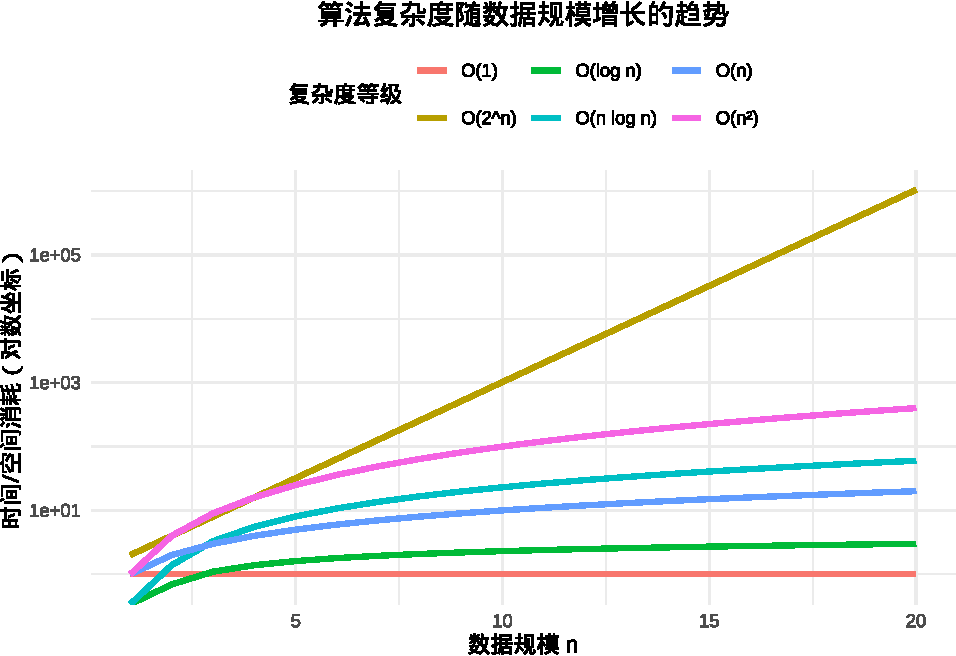
\includegraphics{01-statistical_programing_files/figure-latex/unnamed-chunk-1-1.pdf}

\textbf{结论}:O(1) 和 O(log n) 是极其高效的,O(n) 和 O(n log n) 是优秀的,O(n²) 在 n 较小时可以接受,而 O(2\^{}n) 和 O(n!) 应尽量避免。

\hypertarget{ux7ed9ux6570ux636eux5206ux6790ux5e08ux7684ux542fux793a}{%
\subsubsection{给数据分析师的启示}\label{ux7ed9ux6570ux636eux5206ux6790ux5e08ux7684ux542fux793a}}

\textbf{数据规模是关键}这一认知在生态学数据分析中具有决定性意义。当处理小规模数据集时,算法选择的差异可能并不明显------一个O(n²)的算法在几百条记录上运行可能只需要几毫秒。然而,当数据规模从1万条增长到100万条时,复杂度差异的威力就会充分显现。一个O(n²)的算法(如双重循环进行物种匹配)耗时将增加1万倍,从原本的1秒延长到近3小时;而一个O(n log n)的高效排序算法可能只增加不到20倍,从1秒延长到20秒左右。这种指数级的性能差异决定了某些分析方法在大数据场景下的可行性。在生态学研究中,这意味着我们需要根据预期的数据规模来前瞻性地选择分析方法,而不是等到数据积累到一定规模后再被动调整。

\textbf{理解R语言操作的代价}是生态学数据分析师的核心能力。许多看似简单的R操作背后都隐藏着复杂的算法实现。例如,\texttt{table()}函数用于统计物种频数,其时间复杂度通常是O(n),但当处理大规模数据时仍需注意内存使用;\texttt{merge()}函数进行数据框合并,其复杂度取决于合并策略,可能达到O(n log n)或更高;\texttt{sort()}函数的性能差异更为明显------R默认使用快速排序(平均O(n log n)),但在最坏情况下可能退化到O(n²)。理解这些操作的复杂度特征,能够帮助我们在设计分析流程时做出明智的决策。比如,在处理大型物种分布矩阵时,应该避免在循环内部重复调用\texttt{table()},而是应该预先计算好统计结果。

\textbf{空间换时间}是数据分析中经典的优化策略,在生态学研究中尤为实用。这种策略的核心思想是利用额外的内存存储来避免重复计算,从而显著降低时间复杂度。一个典型的例子是物种多样性分析:如果我们使用双重循环计算所有物种对之间的共存关系,时间复杂度为O(n²);但如果我们先构建一个哈希表(在R中可以使用命名向量或环境对象)存储每个物种的分布信息,然后通过单次遍历完成计算,时间复杂度可以降低到O(n)。虽然这会增加O(n)的空间复杂度,但在现代计算机内存充足的情况下,这种权衡通常是值得的。另一个例子是生态位模型预测:通过预先计算和缓存环境变量的响应曲线,可以避免在预测阶段重复进行复杂的数学运算,从而大幅提升模型运行效率。这种优化思维不仅适用于编程实现,也适用于分析流程设计------通过合理的数据预处理和中间结果存储,我们可以构建既高效又可靠的大规模生态数据分析系统。

\textbf{练习}:尝试分析你写过的一些数据处理脚本,找出其中循环和操作,估算其时间复杂度和空间复杂度。这将极大地提升你的代码质量和性能优化能力。

\hypertarget{aiux534fux540cux7f16ux7a0bux6280ux80fd}{%
\section{AI协同编程技能}\label{aiux534fux540cux7f16ux7a0bux6280ux80fd}}

\hypertarget{aiux7f16ux7a0bux6a21ux5757ux5b89ux88c5}{%
\subsection{AI编程模块安装}\label{aiux7f16ux7a0bux6a21ux5757ux5b89ux88c5}}

大语言模型辅助编程(AI-assisted programming)是当前最热门的AI技术之一,它通过大规模预训练语言模型(如GPT-4、Claude、Qwen等)来协助程序员编写代码。这种技术革命性地改变了编程工作的本质,将程序员从繁琐的语法记忆和重复性编码任务中解放出来,使其能够更专注于算法设计、系统架构和问题解决等高层次思维活动。

然而,大模型训练和调用都需要大量计算资源,这使得AI协作编程的可行性在早期受到限制。直到2025年初DeepSeek等开源模型的出现,普通人AI协作编程的可行性才得到极大提升。随后这种AI辅助编程工具呈现爆发式增长,从最初的GitHub Copilot、DeepSeek,到后来的Claude Code、Codex、Cursor等,几乎每隔几天就有新的工具问世。这种快速迭代反映了AI技术在编程领域的巨大潜力和激烈竞争。

当前AI协作编程工具的种类已经非常丰富,涵盖了从代码补全、错误修复、代码重构到完整功能实现的各个层面。但技术的快速演进也意味着任何具体工具的详细介绍都可能很快过时。因此,本章不追求对特定工具的详尽介绍,而是聚焦于通用的AI协作编程思维框架和核心技能培养。无论使用哪种具体工具,研究者都需要掌握精确提问、代码审查、迭代优化等基本能力。

作为代表性工具,Qwen Code是一个基于大模型的AI协作编程工具,它借鉴了Claude Code的设计理念,支持通过Qwen Coder或Claude Code等大模型来协助编程工作。Qwen Code的特点包括命令行工作流设计、OAuth一键登录、会话管理等功能,为生态学研究者提供了便捷的AI编程协作体验。但更重要的是,通过学习和使用这类工具,研究者能够建立起与AI有效协作的思维模式,这种能力将超越具体工具的局限,成为AI时代生态学数据分析的核心竞争力。

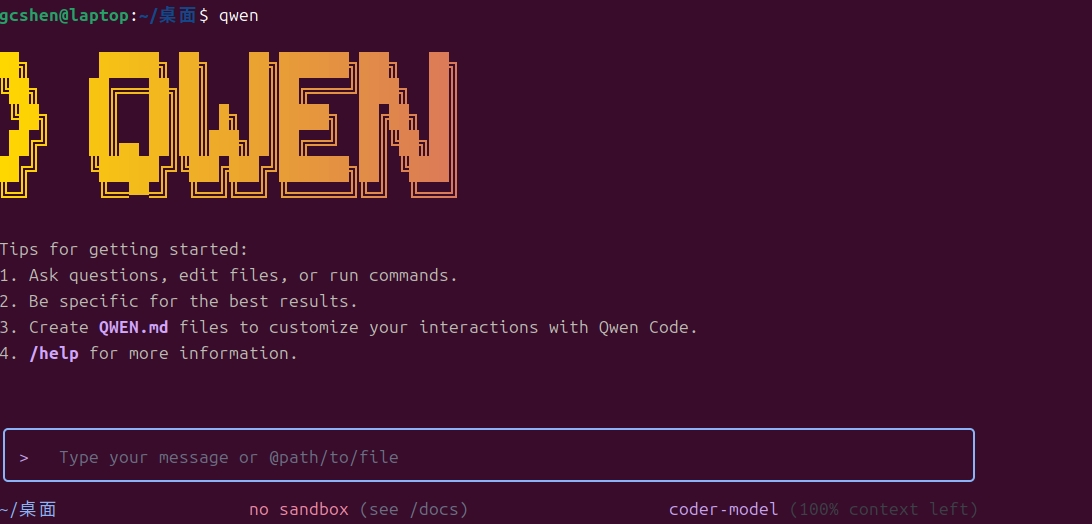
\includegraphics{imgs/qwen-code.jpg}

Qwen Code(阿里通义:\textbf{qwen} 命令的 CLI)

\begin{quote}
明确对标 Claude Code 的命令行工作流工具,对 \textbf{Qwen3-Coder} 优化;支持 \textbf{OAuth 一键登录}(国际/国内均有渠道),也支持 OpenAI-兼容 API;提供 \texttt{/compress}、\texttt{/stats} 等会话管理命令。({[}GitHub{]}{[}8{]})
\end{quote}

\textbf{安装}

\begin{Shaded}
\begin{Highlighting}[]
\CommentTok{\# 需 Node.js 20+}
\ExtensionTok{npm}\NormalTok{ install }\AttributeTok{{-}g}\NormalTok{ @qwen{-}code/qwen{-}code@latest}
\ExtensionTok{qwen} \AttributeTok{{-}{-}version}
\CommentTok{\# 或 Homebrew(macOS/Linux)}
\ExtensionTok{brew}\NormalTok{ install qwen{-}code}
\end{Highlighting}
\end{Shaded}

({[}GitHub{]}{[}8{]})

\textbf{登录(两种模式)}

\begin{Shaded}
\begin{Highlighting}[]
\CommentTok{\# 方式1:Qwen OAuth(零配置,推荐)}
\ExtensionTok{qwen}    \CommentTok{\# 会自动弹浏览器登录 qwen.ai 账户并缓存凭证}

\CommentTok{\# 方式2:OpenAI 兼容 API(适合私有部署/跨地区)}
\BuiltInTok{export} \VariableTok{OPENAI\_API\_KEY}\OperatorTok{=}\NormalTok{...}
\BuiltInTok{export} \VariableTok{OPENAI\_BASE\_URL}\OperatorTok{=}\NormalTok{...    }\CommentTok{\# 例:DashScope/ModelScope/OpenRouter}
\BuiltInTok{export} \VariableTok{OPENAI\_MODEL}\OperatorTok{=}\NormalTok{qwen3{-}coder{-}plus}
\end{Highlighting}
\end{Shaded}

\textbf{上手 \& 常用命令}

\begin{Shaded}
\begin{Highlighting}[]
\BuiltInTok{cd}\NormalTok{ your{-}project}
\ExtensionTok{qwen}
\CommentTok{\# 交互里可以直接自然语言:}
\OperatorTok{\textgreater{}}\NormalTok{ Explain }\ExtensionTok{the}\NormalTok{ codebase structure}
\OperatorTok{\textgreater{}}\NormalTok{ Refactor }\ExtensionTok{this}\NormalTok{ function}
\OperatorTok{\textgreater{}}\NormalTok{ Generate }\ExtensionTok{unit}\NormalTok{ tests}

\CommentTok{\# 会话管理}
\ExtensionTok{/clear}\NormalTok{   /compress   /stats   /exit}
\end{Highlighting}
\end{Shaded}

\textbf{VS Code中集成}

在插件市场吗,搜索 \textbf{Qwen Code} 安装即可。

\hypertarget{ux7cbeux51c6ux63d0ux95eeux6280ux5de7}{%
\subsection{精准提问技巧}\label{ux7cbeux51c6ux63d0ux95eeux6280ux5de7}}

\hypertarget{promptux5de5ux7a0bux57faux672cux539fux5219}{%
\subsubsection{Prompt工程基本原则}\label{promptux5de5ux7a0bux57faux672cux539fux5219}}

\textbf{生态学数据分析的Prompt示例}:

\begin{verbatim}
请用R语言帮我分析森林样地数据:

数据描述:
- 数据框包含以下列:plot_id(样地编号)、species(物种名称)、dbh(胸径)、height(树高)
- 数据已保存在CSV文件中,路径为"data/forest_survey.csv"

分析要求:
1. 读取数据并检查数据质量(缺失值、异常值)
2. 计算每个样地的物种丰富度(物种数)
3. 计算每个样地的平均胸径和平均树高
4. 绘制物种丰富度与平均胸径的关系散点图
5. 使用ggplot2进行可视化,添加适当的标题和标签

请为关键步骤添加注释,并确保代码具有良好的可读性。
\end{verbatim}

\hypertarget{ux4e0aux4e0bux6587ux63d0ux4f9bux4e0eux7ea6ux675fux6761ux4ef6ux8bbeux5b9a}{%
\subsubsection{上下文提供与约束条件设定}\label{ux4e0aux4e0bux6587ux63d0ux4f9bux4e0eux7ea6ux675fux6761ux4ef6ux8bbeux5b9a}}

\textbf{改进的Prompt示例}:

\begin{verbatim}
我正在分析天童森林动态监测样地的数据,需要计算生物多样性指数。

约束条件:
- 数据包含200个固定样地的调查结果
- 每个样地面积为20m×20m
- 只统计DBH≥1cm的木本植物
- 需要排除外来物种和栽培物种

具体要求:
1. 计算每个样地的Shannon-Wiener多样性指数
2. 计算每个样地的Simpson多样性指数
3. 分析多样性指数与海拔的相关性
4. 生成专业的研究报告图表

请使用vegan包进行多样性计算,确保代码符合生态学研究的标准做法。
\end{verbatim}

\hypertarget{ux4ee3ux7801ux5ba1ux67e5ux80fdux529b}{%
\subsection{代码审查能力}\label{ux4ee3ux7801ux5ba1ux67e5ux80fdux529b}}

\hypertarget{llmux8f93ux51faux4ee3ux7801ux7684ux5e38ux89c1ux9519ux8befux7c7bux578b}{%
\subsubsection{LLM输出代码的常见错误类型}\label{llmux8f93ux51faux4ee3ux7801ux7684ux5e38ux89c1ux9519ux8befux7c7bux578b}}

\begin{Shaded}
\begin{Highlighting}[]
\CommentTok{\# LLM可能生成的有问题的代码示例}
\CommentTok{\# 问题1:缺乏错误处理}
\NormalTok{calculate\_density }\OtherTok{\textless{}{-}} \ControlFlowTok{function}\NormalTok{(area, count) \{}
\NormalTok{  density }\OtherTok{\textless{}{-}}\NormalTok{ count }\SpecialCharTok{/}\NormalTok{ area  }\CommentTok{\# 如果area为0会出错}
  \FunctionTok{return}\NormalTok{(density)}
\NormalTok{\}}

\CommentTok{\# 改进版本}
\NormalTok{calculate\_density\_safe }\OtherTok{\textless{}{-}} \ControlFlowTok{function}\NormalTok{(area, count) \{}
  \ControlFlowTok{if}\NormalTok{ (area }\SpecialCharTok{\textless{}=} \DecValTok{0}\NormalTok{) \{}
    \FunctionTok{stop}\NormalTok{(}\StringTok{"面积必须大于0"}\NormalTok{)}
\NormalTok{  \}}
\NormalTok{  density }\OtherTok{\textless{}{-}}\NormalTok{ count }\SpecialCharTok{/}\NormalTok{ area}
  \FunctionTok{return}\NormalTok{(density)}
\NormalTok{\}}

\CommentTok{\# 问题2:使用过时的函数}
\CommentTok{\# LLM可能推荐使用旧的函数版本}
\NormalTok{old\_way }\OtherTok{\textless{}{-}} \FunctionTok{read.table}\NormalTok{(}\StringTok{"data.csv"}\NormalTok{)  }\CommentTok{\# 较老的函数}

\CommentTok{\# 改进:使用更现代的tidyverse方法}
\FunctionTok{library}\NormalTok{(tidyverse)}
\NormalTok{modern\_way }\OtherTok{\textless{}{-}} \FunctionTok{read\_csv}\NormalTok{(}\StringTok{"data.csv"}\NormalTok{)  }\CommentTok{\# 更简洁的语法}
\end{Highlighting}
\end{Shaded}

\hypertarget{ux529fux80fdux6b63ux786eux6027ux9a8cux8bc1ux65b9ux6cd5}{%
\subsubsection{功能正确性验证方法}\label{ux529fux80fdux6b63ux786eux6027ux9a8cux8bc1ux65b9ux6cd5}}

\begin{Shaded}
\begin{Highlighting}[]
\CommentTok{\# 创建测试用例验证函数正确性}
\NormalTok{test\_diversity\_calculation }\OtherTok{\textless{}{-}} \ControlFlowTok{function}\NormalTok{() \{}
  \CommentTok{\# 测试用例1:单一物种}
\NormalTok{  single\_species }\OtherTok{\textless{}{-}} \FunctionTok{rep}\NormalTok{(}\StringTok{"Oak"}\NormalTok{, }\DecValTok{10}\NormalTok{)}
\NormalTok{  result1 }\OtherTok{\textless{}{-}} \FunctionTok{calculate\_diversity}\NormalTok{(single\_species)}

  \CommentTok{\# 单一物种的Shannon指数应该为0}
  \ControlFlowTok{if}\NormalTok{ (}\FunctionTok{abs}\NormalTok{(result1}\SpecialCharTok{$}\NormalTok{shannon }\SpecialCharTok{{-}} \DecValTok{0}\NormalTok{) }\SpecialCharTok{\textgreater{}} \FloatTok{1e{-}10}\NormalTok{) \{}
    \FunctionTok{stop}\NormalTok{(}\StringTok{"单一物种测试失败"}\NormalTok{)}
\NormalTok{  \}}

  \CommentTok{\# 测试用例2:两个物种各占一半}
\NormalTok{  two\_species }\OtherTok{\textless{}{-}} \FunctionTok{rep}\NormalTok{(}\FunctionTok{c}\NormalTok{(}\StringTok{"Oak"}\NormalTok{, }\StringTok{"Pine"}\NormalTok{), }\AttributeTok{each =} \DecValTok{5}\NormalTok{)}
\NormalTok{  result2 }\OtherTok{\textless{}{-}} \FunctionTok{calculate\_diversity}\NormalTok{(two\_species)}

  \CommentTok{\# 两个物种各占一半的Shannon指数应该为log(2)}
\NormalTok{  expected }\OtherTok{\textless{}{-}} \FunctionTok{log}\NormalTok{(}\DecValTok{2}\NormalTok{)}
  \ControlFlowTok{if}\NormalTok{ (}\FunctionTok{abs}\NormalTok{(result2}\SpecialCharTok{$}\NormalTok{shannon }\SpecialCharTok{{-}}\NormalTok{ expected) }\SpecialCharTok{\textgreater{}} \FloatTok{1e{-}10}\NormalTok{) \{}
    \FunctionTok{stop}\NormalTok{(}\StringTok{"两个物种测试失败"}\NormalTok{)}
\NormalTok{  \}}

  \FunctionTok{cat}\NormalTok{(}\StringTok{"所有测试通过!}\SpecialCharTok{\textbackslash{}n}\StringTok{"}\NormalTok{)}
\NormalTok{\}}

\CommentTok{\# 运行测试}
\FunctionTok{test\_diversity\_calculation}\NormalTok{()}
\end{Highlighting}
\end{Shaded}

\hypertarget{ux8c03ux8bd5ux4e0eux9519ux8befux5904ux7406}{%
\subsection{调试与错误处理}\label{ux8c03ux8bd5ux4e0eux9519ux8befux5904ux7406}}

\hypertarget{ux9519ux8befux4fe1ux606fux89e3ux8bfbux4e0eux5b9aux4f4d}{%
\subsubsection{错误信息解读与定位}\label{ux9519ux8befux4fe1ux606fux89e3ux8bfbux4e0eux5b9aux4f4d}}

\begin{Shaded}
\begin{Highlighting}[]
\CommentTok{\# 常见的R错误信息及解决方法}

\CommentTok{\# 错误1:对象未找到}
\CommentTok{\# Error: object \textquotesingle{}x\textquotesingle{} not found}
\CommentTok{\# 解决方法:检查变量名拼写,确保变量已赋值}

\CommentTok{\# 错误2:函数参数不匹配}
\CommentTok{\# Error in mean(x) : 参数不是数值也不是逻辑值:回传NA}
\CommentTok{\# 解决方法:检查数据类型,确保输入是数值型}

\CommentTok{\# 错误3:下标越界}
\CommentTok{\# Error in x[5] : 下标出界}
\CommentTok{\# 解决方法:检查向量长度,确保索引在有效范围内}

\CommentTok{\# 实用的调试技巧}
\NormalTok{debug\_calculation }\OtherTok{\textless{}{-}} \ControlFlowTok{function}\NormalTok{(data) \{}
  \CommentTok{\# 使用browser()进行交互式调试}
  \FunctionTok{browser}\NormalTok{()}

\NormalTok{  result }\OtherTok{\textless{}{-}} \FunctionTok{complex\_calculation}\NormalTok{(data)}
  \FunctionTok{return}\NormalTok{(result)}
\NormalTok{\}}

\CommentTok{\# 使用tryCatch处理错误}
\NormalTok{safe\_calculation }\OtherTok{\textless{}{-}} \ControlFlowTok{function}\NormalTok{(data) \{}
\NormalTok{  result }\OtherTok{\textless{}{-}} \FunctionTok{tryCatch}\NormalTok{(\{}
    \CommentTok{\# 尝试执行可能出错的操作}
    \FunctionTok{calculate\_diversity}\NormalTok{(data)}
\NormalTok{  \}, }\AttributeTok{error =} \ControlFlowTok{function}\NormalTok{(e) \{}
    \CommentTok{\# 错误处理}
    \FunctionTok{cat}\NormalTok{(}\StringTok{"计算失败:"}\NormalTok{, e}\SpecialCharTok{$}\NormalTok{message, }\StringTok{"}\SpecialCharTok{\textbackslash{}n}\StringTok{"}\NormalTok{)}
    \FunctionTok{return}\NormalTok{(}\ConstantTok{NULL}\NormalTok{)}
\NormalTok{  \}, }\AttributeTok{warning =} \ControlFlowTok{function}\NormalTok{(w) \{}
    \CommentTok{\# 警告处理}
    \FunctionTok{cat}\NormalTok{(}\StringTok{"警告:"}\NormalTok{, w}\SpecialCharTok{$}\NormalTok{message, }\StringTok{"}\SpecialCharTok{\textbackslash{}n}\StringTok{"}\NormalTok{)}
    \FunctionTok{return}\NormalTok{(}\FunctionTok{calculate\_diversity}\NormalTok{(data))  }\CommentTok{\# 继续执行}
\NormalTok{  \})}

  \FunctionTok{return}\NormalTok{(result)}
\NormalTok{\}}
\end{Highlighting}
\end{Shaded}

\hypertarget{ux603bux7ed3}{%
\section{总结}\label{ux603bux7ed3}}

本章系统性地构建了AI时代生态学统计编程的全新教育框架,标志着编程教育从''技能导向''向''思维导向''的根本性转变。在大语言模型成为强大编程助手的今天,编程教育的核心价值已不再体现在语法记忆和API细节掌握上,而是转向更高层次的思维能力培养。

本章重点培养了两大核心能力体系:首先是\textbf{高阶思维与问题解决能力},包括问题分解与抽象建模能力、算法与数据结构思维、数据分析流程设计与规划能力。这些能力构成了生态学研究者驾驭AI工具的''方向盘'',确保研究者能够站在战略高度设计分析方案,而不仅仅是执行具体的编程任务。其次是\textbf{与LLM协同工作的能力},涵盖精确提问与Prompt工程、代码审查与批判性验证、迭代与优化等关键技能,这些能力使研究者能够有效指导AI完成复杂的数据分析任务。

在技术层面,本章通过模块化的学习路径,系统介绍了通用编程思维基础,包括变量与常量、数据类型、运算符、集合数据类型、分支与循环、函数、作用域、错误处理、模块化、面向对象、内存管理、测试和代码规范等核心概念。这些知识为生态学数据分析提供了坚实的技术基础,确保研究者能够理解计算的基本原理,而不仅仅是记忆特定工具的使用方法。

特别值得强调的是,本章提出的''分析方案设计师 + AI指令员 + 质量保证官''三位一体的角色定位,精准地捕捉了AI时代生态学研究者的核心竞争力。研究者不再需要为琐碎的编程细节所困扰,而是将精力集中在更具价值的分析设计、方法选择和结果解释上。这种角色转变不仅提高了研究效率,更提升了研究的科学性和创新性。

通过本章的学习,学生将建立起现代数据分析的思维框架,能够将复杂的生态学问题转化为清晰可执行的分析流程,并利用AI工具高效实现技术方案。这种能力框架具有高度的通用性和适应性,不仅适用于当前的R语言生态,也为未来学习其他编程语言和分析工具奠定了坚实基础。

在后续章节中,我们将基于本章建立的编程思维框架,深入探讨更专业的生态统计方法。但无论技术工具如何发展,本章所强调的分析思维、问题解决能力和AI协作素养,都将成为生态学研究者应对技术变革、推动学科发展的核心竞争优势。这种以思维为导向的编程教育,正是培养未来生态学创新人才的关键路径。

\hypertarget{ux7efcux5408ux7ec3ux4e60}{%
\section{综合练习}\label{ux7efcux5408ux7ec3ux4e60}}

\hypertarget{ux7ec3ux4e601}{%
\subsection{练习1}\label{ux7ec3ux4e601}}

请在AI的协助下,判断项目data目录下的Tiantong\_Sample.CSV文件内的所有树木空间位置是否是随机分布?请注意,写完代码和出了结果后,并不代表该习题的结束。你需要在AI的协助下,理解其分析思路,每行代码的意思。下堂课会随机请人上来讲解。

\hypertarget{ux6982ux7387ux4e0eux5206ux5e03}{%
\chapter{概率与分布}\label{ux6982ux7387ux4e0eux5206ux5e03}}

\hypertarget{ux8682ux86b1ux5348ux9910ux4e0eux6982ux7387}{%
\section{蚂蚱午餐与概率}\label{ux8682ux86b1ux5348ux9910ux4e0eux6982ux7387}}

\hypertarget{ux4e00ux53eaux86b1ux8722ux7684ux5348ux9910}{%
\subsection{一只蚱蜢的午餐}\label{ux4e00ux53eaux86b1ux8722ux7684ux5348ux9910}}

想象一下,你是校园里一只普通的蚱蜢。在你面前,是三片不同的草地:一片是茂盛的黑麦草,一片是点缀着雏菊的混合草甸,另一片则是以三叶草为主。对你来说,这不仅仅是风景,而是你的''餐桌''。现在,我要向你提出一个看似简单,实则充满了不确定性的问题:你下一顿午餐,会选择在哪一种植物上进食?

这个简单的问题背后,隐藏着生态学研究的核心挑战------如何理解和量化生物行为中的不确定性。你的选择可能受到多种因素的影响:黑麦草的高营养价值、混合草甸的隐蔽性、三叶草的特殊口感,甚至是当天的天气、你的饥饿程度,或是周围是否有捕食者。每一个微小的变量都可能改变你的最终决定。

作为一名生态学从业者,我的任务就是量化你的这种''选择偏好''。而这个''偏好'',本质上就是\textbf{概率}------一个介于0和1之间的数字,用来描述某个不确定事件(蚱蜢选择某种植物)发生的可能性。概率为0意味着绝不可能,概率为1意味着必然发生。但现实世界中的概率往往介于这两个极端之间,反映了生物决策中的复杂性和随机性。

那么,我该如何度量和理解你这只蚱蜢的''选择概率''呢?这不仅仅是简单的计数问题,而是需要建立数学模型来描述你的行为模式。概率理论为我们提供了三种不同的视角来理解这种不确定性:基于理想假设的古典概率、基于实际观察的频率概率,以及能够结合新证据不断更新认知的贝叶斯概率。每一种方法都有其独特的价值和适用场景,共同构成了我们理解自然界的数学工具箱。

\hypertarget{ux7406ux60f3ux7684ux731cux6d4bux53e4ux5178ux6982ux7387}{%
\subsection{理想的猜测------古典概率}\label{ux7406ux60f3ux7684ux731cux6d4bux53e4ux5178ux6982ux7387}}

一开始,我没有任何观察数据。我只能基于``公平原则''进行一个理想化的猜测。我发现,你活动的区域里,黑麦草、混合草甸和三叶草的面积恰好相等。于是,我假设你选择任何一种植物的可能性都是完全一样的。

\begin{itemize}
\tightlist
\item
  \textbf{这就是古典概率(先验概率)。} 它的核心是``等可能性''。在这个理想模型里,有三种可能的结果,且每一种结果出现的可能性相同。
\item
  \textbf{计算公式是:} \[P(\text{蚱蜢选择黑麦草}) = \frac{\text{有利于该事件的结果数}}{\text{所有可能的结果数}} = \frac{1}{3}\]
\item
  这种概率源于逻辑推理,而非实际数据。它简洁优美,但现实世界往往并非如此``公平''。毕竟,你可能就是偏爱某种口味呢?
\end{itemize}

\hypertarget{ux6838ux5fc3ux601dux60f3ux7b49ux53efux80fdux6027}{%
\subsubsection{核心思想:等可能性}\label{ux6838ux5fc3ux601dux60f3ux7b49ux53efux80fdux6027}}

想象一下,你正在和一位朋友玩一个完全公平的掷骰子游戏。骰子质地均匀,形状完美。那么,在掷出之前,你会认为掷出``1点''的可能性有多大?你的直觉很可能会告诉你:六分之一。

支撑这个直觉的,就是古典概率(也称为先验概率)的思维方式。它是概率论中最古老、最直观的定义,源于对如赌博等机会游戏的研究。古典概率的历史可以追溯到17世纪,当时法国数学家布莱兹·帕斯卡和皮埃尔·德·费马通过书信往来,共同解决了赌博中的概率问题,为现代概率论奠定了基础。

古典概率的核心前提是 ``等可能性''。即一个随机试验的所有可能结果,发生的可能性必须完全相同。这个假设看似简单,实则蕴含着深刻的数学哲学思想。等可能性的概念建立在对称性原则之上。当我们说一个骰子的六个面''等可能''时,实际上是在说这个骰子在几何形状、质量分布等方面具有完美的对称性。这种对称性确保了每个面朝上的物理条件完全相同。

在生态学中,等可能性的假设意味着我们暂时忽略了所有可能影响生物选择的因素,将系统简化为一个完全随机的过程。这种简化虽然不完美,但为我们提供了一个理论基准,帮助我们理解''如果世界是完全随机的,会发生什么''。

\hypertarget{ux5b9aux4e49ux4e0eux516cux5f0f}{%
\subsubsection{定义与公式}\label{ux5b9aux4e49ux4e0eux516cux5f0f}}

在满足``等可能性''的试验中,我们称每个单一的可能结果为一个 ``\textbf{基本事件}'' 。所有基本事件构成的集合,就是 ``\textbf{样本空间}''。样本空间的概念是概率论的基础,它定义了所有可能发生的结果。

构建样本空间需要仔细考虑试验的所有可能结果。例如,在蚱蜢选择植物的例子中,样本空间包含三个基本事件:\{选择黑麦草,选择混合草甸,选择三叶草\}。每个基本事件都是互斥且完备的------互斥意味着不可能同时发生两个事件,完备意味着涵盖了所有可能性。

古典概率的定义公式简洁而优美:

\[P(A) = \frac{\text{事件A包含的基本事件个数}}{\text{样本空间中基本事件的总数}}\]

\(P(A)\): 事件A发生的概率。分子: 你关心的事件A包含了多少种可能的结果。分母: 整个试验一共有多少种可能的结果。

这个公式计算出的概率,是一个介于0和1之间的数。\(P(A)=0\)表示事件A不可能发生;\(P(A)=1\)表示事件A必然发生。概率的归一化条件要求所有基本事件的概率之和等于1。

\hypertarget{ux6982ux7387ux7684ux4e09ux4e2aux57faux672cux5c5eux6027}{%
\subsubsection{概率的三个基本属性}\label{ux6982ux7387ux7684ux4e09ux4e2aux57faux672cux5c5eux6027}}

无论采用哪种概率定义(古典、频率或贝叶斯),概率都必须满足三个基本公理,这些公理由俄罗斯数学家安德雷·柯尔莫哥洛夫在1933年提出,为现代概率论奠定了坚实的数学基础。

\textbf{公理1:非负性}
对于任意事件A,其概率总是非负的:
\[P(A) \geq 0\]

这个公理确保了概率的合理性。在生态学中,这意味着任何生态事件的发生概率都不可能为负值,无论这个事件多么罕见或不可能。

\textbf{公理2:规范性}
整个样本空间的概率为1:
\[P(\Omega) = 1\]

其中\(\Omega\)表示样本空间,即所有可能结果的集合。这个公理表明''必然事件''的概率为1。在蚱蜢的例子中,样本空间包含三种植物选择,因此\(P(\text{选择任意植物}) = 1\)。

\textbf{公理3:可加性}
对于任意两个互斥事件A和B(即A和B不能同时发生):
\[P(A \cup B) = P(A) + P(B)\]

这个公理可以推广到有限个或可数无限个互斥事件。在生态学中,这意味着如果两个生态事件不可能同时发生(如''蚱蜢同时选择黑麦草和混合草甸''),那么它们中至少有一个发生的概率等于各自概率之和。

这三个公理共同构成了概率论的数学基础,确保了概率计算的逻辑一致性。从这些基本公理出发,我们可以推导出概率的所有其他性质,如:
- \(P(A^c) = 1 - P(A)\)(互补事件的概率)
- 如果\(A \subseteq B\),则\(P(A) \leq P(B)\)(概率的单调性)
- \(P(A \cup B) = P(A) + P(B) - P(A \cap B)\)(一般加法公式)

这些性质在生态学研究中具有重要的应用价值,帮助我们建立合理的概率模型并进行正确的统计推断。

\hypertarget{ux751fux6001ux5b66ux4e2dux7684ux53e4ux5178ux6982ux7387ux5e94ux7528}{%
\subsubsection{生态学中的古典概率应用}\label{ux751fux6001ux5b66ux4e2dux7684ux53e4ux5178ux6982ux7387ux5e94ux7528}}

尽管古典概率的假设很强,但在某些生态学场景中仍然有其应用价值:

\textbf{1. 理想化的种群分布模型}

当我们研究物种在栖息地中的分布时,可以先建立一个''等可能性''的基准模型。例如,假设一个森林中有三种不同类型的微生境(阳光充足区、半阴区、全阴区),我们可以先假设物种在这三种生境中出现的概率相等,然后与实际观测数据进行比较。这种比较可以帮助我们识别物种的真实偏好。

\textbf{2. 随机抽样设计}

在生态调查中,我们经常需要随机选择样方位置。如果样方选择过程真正实现了''等可能性'',那么每个位置被选中的概率应该完全相同。这种设计确保了样本的代表性,避免了选择偏差。

\textbf{3. 遗传学中的孟德尔定律}

在种群遗传学中,孟德尔的遗传定律实际上就是基于古典概率的等可能性假设。当亲本的基因型确定后,子代获得特定基因组合的概率可以通过古典概率计算。

\hypertarget{ux53e4ux5178ux6982ux7387ux7684ux5c40ux9650ux6027}{%
\subsubsection{古典概率的局限性}\label{ux53e4ux5178ux6982ux7387ux7684ux5c40ux9650ux6027}}

尽管古典概率模型非常优美,但它的''理想化''也恰恰是它在现实应用中的主要局限:

\textbf{1. ``等可能性''假设过于苛刻}

现实世界中,很多情况不满足等可能性。生态系统的复杂性使得''等可能性''的假设往往过于简化:

回到蚱蜢的例子: 我们能说蚱蜢选择黑麦草、混合草甸和三叶草的可能性完全相等吗?几乎不能!植物的营养价值、口感、防御性化学物质、空间分布、季节变化等因素都存在差异,这些都会破坏''等可能性''假设。

一枚实际硬币: 可能因工艺瑕疵导致正面和反面出现的概率并非精确的50\%。研究表明,大多数硬币实际上有51\%-49\%的轻微偏差。

一只青蛙选择池塘: 池塘的大小、水深、水质、是否有天敌、食物丰富度等因素必然会影响其选择,使得''等可能性''的假设不成立。

\textbf{2. 样本空间必须是有限集合}

古典概率要求可能的结果是有限可数的。对于连续性的问题(如蚱蜢的精确跳跃距离是1.253米),因为结果有无限多个,古典概率便无能为力。生态学中的许多测量值都是连续变量,如温度、湿度、生物量等,这些都需要连续概率分布来描述。古典概率还要求明确知道总体大小,但生态学中总体往往无限或未知:

\begin{Shaded}
\begin{Highlighting}[]
\CommentTok{\# 有限总体问题示例:估计森林中濒危物种的数量}
\FunctionTok{set.seed}\NormalTok{(}\DecValTok{222}\NormalTok{)}

\CommentTok{\# 实际濒危物种数量(未知)}
\NormalTok{true\_rare\_species }\OtherTok{\textless{}{-}} \DecValTok{15}

\CommentTok{\# 调查发现的物种数量(抽样偏差)}
\NormalTok{observed\_species }\OtherTok{\textless{}{-}} \DecValTok{8}
\NormalTok{survey\_effort }\OtherTok{\textless{}{-}} \DecValTok{50}  \CommentTok{\# 调查努力程度}

\NormalTok{detection\_prob }\OtherTok{\textless{}{-}}\NormalTok{ observed\_species }\SpecialCharTok{/}\NormalTok{ survey\_effort}
\NormalTok{estimated\_total }\OtherTok{\textless{}{-}}\NormalTok{ observed\_species }\SpecialCharTok{/}\NormalTok{ detection\_prob}

\FunctionTok{cat}\NormalTok{(}\StringTok{"实际濒危物种数量:"}\NormalTok{, true\_rare\_species, }\StringTok{"}\SpecialCharTok{\textbackslash{}n}\StringTok{"}\NormalTok{)}
\end{Highlighting}
\end{Shaded}

\begin{verbatim}
## 实际濒危物种数量: 15
\end{verbatim}

\begin{Shaded}
\begin{Highlighting}[]
\FunctionTok{cat}\NormalTok{(}\StringTok{"观测到的物种数量:"}\NormalTok{, observed\_species, }\StringTok{"}\SpecialCharTok{\textbackslash{}n}\StringTok{"}\NormalTok{)}
\end{Highlighting}
\end{Shaded}

\begin{verbatim}
## 观测到的物种数量: 8
\end{verbatim}

\begin{Shaded}
\begin{Highlighting}[]
\FunctionTok{cat}\NormalTok{(}\StringTok{"检测概率:"}\NormalTok{, }\FunctionTok{round}\NormalTok{(detection\_prob, }\DecValTok{3}\NormalTok{), }\StringTok{"}\SpecialCharTok{\textbackslash{}n}\StringTok{"}\NormalTok{)}
\end{Highlighting}
\end{Shaded}

\begin{verbatim}
## 检测概率: 0.16
\end{verbatim}

\begin{Shaded}
\begin{Highlighting}[]
\FunctionTok{cat}\NormalTok{(}\StringTok{"估计的物种总数:"}\NormalTok{, }\FunctionTok{round}\NormalTok{(estimated\_total, }\DecValTok{1}\NormalTok{), }\StringTok{"}\SpecialCharTok{\textbackslash{}n}\StringTok{"}\NormalTok{)}
\end{Highlighting}
\end{Shaded}

\begin{verbatim}
## 估计的物种总数: 50
\end{verbatim}

\begin{Shaded}
\begin{Highlighting}[]
\FunctionTok{cat}\NormalTok{(}\StringTok{"估计误差:"}\NormalTok{, }\FunctionTok{round}\NormalTok{(}\FunctionTok{abs}\NormalTok{(estimated\_total }\SpecialCharTok{{-}}\NormalTok{ true\_rare\_species), }\DecValTok{1}\NormalTok{), }\StringTok{"}\SpecialCharTok{\textbackslash{}n}\StringTok{"}\NormalTok{)}
\end{Highlighting}
\end{Shaded}

\begin{verbatim}
## 估计误差: 35
\end{verbatim}

\textbf{3. 无法处理主观概率}

古典概率是客观的,基于计数。但它无法处理如''我认为明天会下雨的可能性是70\%``这种基于个人知识、经验和信念的主观判断。在生态学预测中,专家意见和经验判断往往很重要,但这些主观因素无法用古典概率来量化。

\textbf{4. 忽略历史依赖性和学习效应}

古典概率假设每次试验都是独立的,但生物行为往往具有记忆性和学习能力。如果蚱蜢昨天在黑麦草上获得了丰富的营养,它今天更可能再次选择黑麦草。这种历史依赖性破坏了古典概率的独立性假设。

\hypertarget{ux4eceux53e4ux5178ux6982ux7387ux5230ux73b0ux4ee3ux6982ux7387ux8bba}{%
\subsubsection{从古典概率到现代概率论}\label{ux4eceux53e4ux5178ux6982ux7387ux5230ux73b0ux4ee3ux6982ux7387ux8bba}}

古典概率虽然简单,但它为现代概率论的发展奠定了基础。20世纪初,俄罗斯数学家安德雷·柯尔莫哥洛夫建立了概率论的公理化体系,将概率定义为满足特定性质的测度函数。这个公理化体系能够同时涵盖古典概率、几何概率和统计概率,为概率论提供了坚实的数学基础。

总结来说,古典概率如同几何学中的完美圆规和直尺,它描绘了一个规则、公平、易于理解的理想世界。它是我们概率之旅的起点,教会我们''计数''的重要性,培养了我们对随机现象的基本直觉。当我们告别这个理想世界,步入充满复杂性和不确定性的真实生态学领域时,频率概率和贝叶斯概率等更强大的工具便会接过接力棒,帮助我们更好地刻画那只真实蚱蜢的、受到多种因素影响的午餐选择。古典概率的价值不在于它的现实准确性,而在于它为我们的思维提供了一个清晰的起点和参照系。

\hypertarget{ux6570ux636eux7684ux8bedux8a00ux9891ux7387ux6982ux7387}{%
\subsection{数据的语言------频率概率}\label{ux6570ux636eux7684ux8bedux8a00ux9891ux7387ux6982ux7387}}

为了了解真相,我决定进行实地观察。我在一周里,每天中午记录你进食的位置,一共记录了70次选择。数据如下:45次在黑麦草上,20次在混合草甸上,5次在三叶草上。

\begin{itemize}
\tightlist
\item
  \textbf{这时,我使用的是频率概率。} 它的核心思想是:一个事件发生的概率,等于它在长期重复试验中出现的\textbf{频率}。
\item
  \textbf{度量方式为:} \(P(\text{选择黑麦草}) \approx \frac{45}{70} \approx 0.64\); \(P(\text{选择混合草甸}) \approx \frac{20}{70} \approx 0.29\); \(P(\text{选择三叶草}) \approx \frac{5}{70} \approx 0.07\)。
\item
  这些数字(0.64, 0.29, 0.07)就是基于客观数据对你进食偏好的\textbf{度量}。它们告诉我,你的偏好并非均等,而是对黑麦草有强烈的倾向性。\textbf{大数定律}在这里默默起作用:观察的次数越多,这个频率就会越稳定地接近你内在的、真实的''偏好概率''。
\end{itemize}

\hypertarget{ux6838ux5fc3ux601dux60f3ux7ecfux9a8cux4e3bux4e49ux4e0eux91cdux590dux8bd5ux9a8c}{%
\subsubsection{核心思想:经验主义与重复试验}\label{ux6838ux5fc3ux601dux60f3ux7ecfux9a8cux4e3bux4e49ux4e0eux91cdux590dux8bd5ux9a8c}}

频率概率(也称为统计概率)的核心思想源于经验主义哲学------知识来自于观察和经验。与古典概率的''先验''推理不同,频率概率是''后验''的,它基于实际收集的数据。

\textbf{大数定律的数学基础}

大数定律是频率概率的理论支柱。这个定律告诉我们:当试验次数足够多时,事件发生的频率会稳定地趋近于其真实的概率。这种稳定性不是偶然的,而是概率论的基本规律。

在生态学中,频率概率意味着我们通过系统的观察来了解生物行为的真实模式。每一次观察都是对''真实概率''的一次逼近,随着观察次数的增加,我们的估计会越来越准确。

概率收敛理论是统计推断的数学基础,帮助我们理解样本统计量如何趋近于总体参数。

\begin{verbatim}
## Loading required package: sysfonts
\end{verbatim}

\begin{verbatim}
## Loading required package: showtextdb
\end{verbatim}

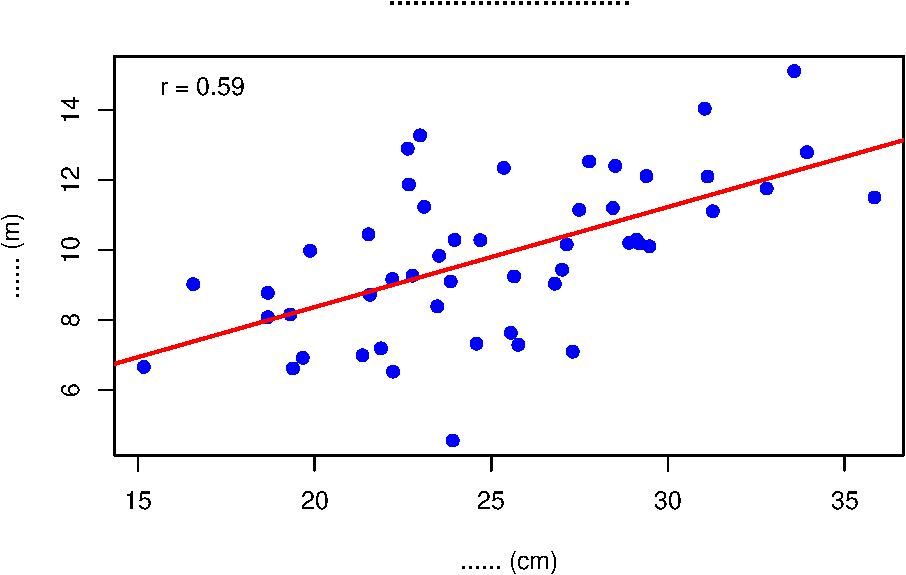
\includegraphics{02-probability_and_distribution_files/figure-latex/unnamed-chunk-2-1.pdf}

\textbf{频率概率的现实类比}

就像天气预报:气象学家通过分析多年的气象数据,得出某地区在特定季节下雨的概率。

就像质量控制:工厂通过检测大量产品的质量,估计产品合格率。

就像医学研究:通过大规模的临床试验,确定某种药物的有效率。

频率概率让我们从''理想世界''走向''真实世界'',用数据说话,用事实说话。

\hypertarget{ux5b9aux4e49ux4e0eux8ba1ux7b97ux65b9ux6cd5}{%
\subsubsection{定义与计算方法}\label{ux5b9aux4e49ux4e0eux8ba1ux7b97ux65b9ux6cd5}}

频率概率的定义基于长期重复试验的思想。对于一个随机事件A,其频率概率定义为:

\[P(A) = \lim_{n \to \infty} \left( \frac{\text{事件A发生的次数}}{\text{总试验次数}} \right)\]

其中\(n\)表示试验的总次数。在实际应用中,我们通常用有限次试验的频率来近似真实的概率:

\[P(A) \approx \frac{\text{事件A发生的次数}}{\text{总试验次数}}\]

\textbf{频率概率的计算步骤}

\begin{enumerate}
\def\labelenumi{\arabic{enumi}.}
\item
  \textbf{设计观察方案}:确定观察的时间、地点、方法,确保观察的系统性和代表性。
\item
  \textbf{收集数据}:按照设计方案进行重复观察,记录每次试验的结果。
\item
  \textbf{统计频率}:计算事件发生的次数与总观察次数的比值。
\item
  \textbf{评估可靠性}:根据样本大小评估估计的可靠性,样本越大,估计越准确。
\end{enumerate}

\textbf{样本大小的重要性}

在频率概率中,样本大小(观察次数)至关重要。小样本可能受到随机波动的影响,而大样本能够更好地反映真实的概率分布。生态学研究通常需要足够的样本量来获得可靠的估计。

\hypertarget{ux751fux6001ux5b66ux4e2dux7684ux9891ux7387ux6982ux7387ux5e94ux7528}{%
\subsubsection{生态学中的频率概率应用}\label{ux751fux6001ux5b66ux4e2dux7684ux9891ux7387ux6982ux7387ux5e94ux7528}}

频率概率在生态学研究中有着广泛的应用:

\textbf{1. 种群密度估计}

通过样方法调查物种在特定区域的分布频率,可以估计整个种群的密度。例如,在100个样方中发现目标物种的样方比例为30\%,可以推断该物种在整个区域的分布概率约为30\%。

\textbf{2. 行为生态学研究}

通过观察动物行为的频率,可以量化其行为偏好。例如,观察鸟类在不同树种上筑巢的频率,可以了解其对栖息地的选择偏好。

\textbf{3. 物种分布模型}

基于物种在不同环境条件下的出现频率,可以建立物种分布模型,预测物种在未调查区域的分布概率。

\textbf{4. 生态风险评估}

通过分析历史数据中不利事件(如物种灭绝、生态系统崩溃)的发生频率,可以评估未来的生态风险。

\hypertarget{ux9891ux7387ux6982ux7387ux7684ux4f18ux52bfux4e0eux5c40ux9650ux6027}{%
\subsubsection{频率概率的优势与局限性}\label{ux9891ux7387ux6982ux7387ux7684ux4f18ux52bfux4e0eux5c40ux9650ux6027}}

频率概率方法在生态学研究中展现出显著的优势。首先,其\textbf{客观性}确保了概率估计基于实际观察数据而非主观臆断,这为生态学研究提供了坚实的实证基础。通过系统记录生物行为或环境变化,研究者能够获得反映真实世界规律的量化结果。其次,频率概率具有\textbf{可验证性},任何研究者都可以通过重复相同的观察或实验来验证结果的可靠性,这符合科学研究的可重复性原则。在\textbf{实用性}方面,频率概率适用于各种现实世界的概率估计问题,从物种分布调查到种群动态监测,都能提供有效的量化工具。最重要的是,频率概率具有\textbf{渐进精确性},随着样本量的增加,根据大数定律,频率估计会越来越接近真实的概率值,这种自我修正的特性使其成为长期生态监测的理想工具。

然而,频率概率方法也存在明显的局限性。\textbf{需要大量数据}是其最突出的限制,为了获得可靠的估计,通常需要大量的观察数据,这在某些稀有物种或难以观察的行为研究中可能难以实现。\textbf{无法处理一次性事件}是另一个重要局限,对于无法重复的事件(如特定物种的灭绝、罕见自然灾害等),频率概率难以提供有意义的估计。\textbf{历史依赖性}使得基于历史数据的概率估计可能无法准确反映未来的变化,特别是在环境快速变化的背景下,过去的数据可能无法预测未来的趋势。此外,\textbf{样本偏差}问题不容忽视,如果样本选择不具有代表性,或者观察过程中存在系统性偏差,频率估计会产生误导性的结果。这些局限性提醒我们在应用频率概率时需要谨慎考虑其适用条件,并在必要时结合其他概率方法进行综合分析。

频率概率需要大量重复试验,但生态学调查往往样本量有限:

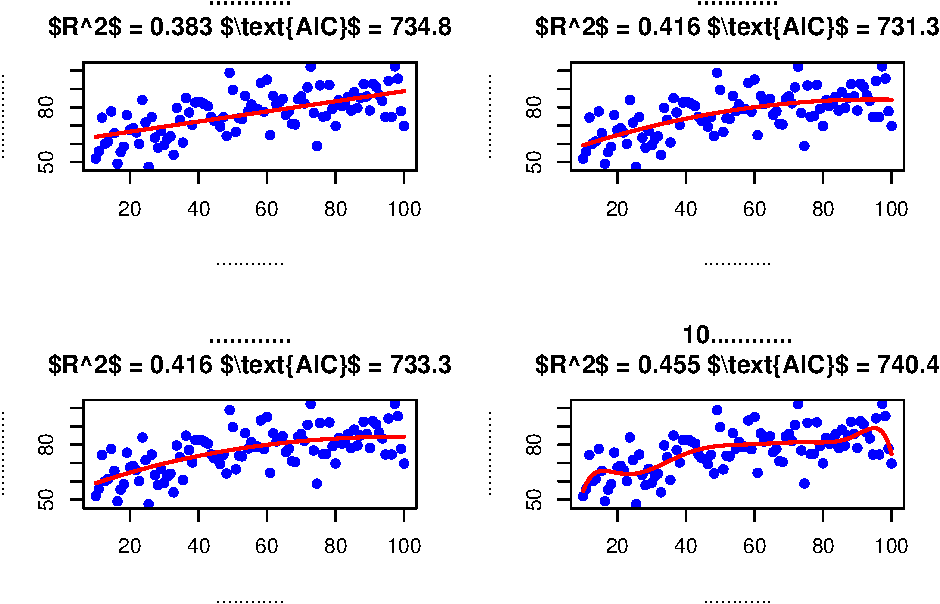
\includegraphics{02-probability_and_distribution_files/figure-latex/unnamed-chunk-3-1.pdf}

\hypertarget{ux4eceux9891ux7387ux6982ux7387ux5230ux73b0ux4ee3ux7edfux8ba1ux5b66}{%
\subsubsection{从频率概率到现代统计学}\label{ux4eceux9891ux7387ux6982ux7387ux5230ux73b0ux4ee3ux7edfux8ba1ux5b66}}

频率概率为现代统计学的发展奠定了基础。统计推断中的参数估计、假设检验等方法都建立在频率概率的思想之上。20世纪,罗纳德·费希尔、耶日·内曼等统计学家进一步发展了频率统计学的理论体系。

总结来说,频率概率如同生态学家的''望远镜'',让我们能够通过系统的观察来窥见自然界的真实规律。它教会我们''用数据说话''的重要性,培养了我们对实证研究的尊重。当我们面对复杂的生态系统时,频率概率为我们提供了量化不确定性的有力工具,帮助我们基于客观证据做出科学的判断。

\hypertarget{ux52a8ux6001ux7684ux66f4ux65b0ux8d1dux53f6ux65afux6982ux7387}{%
\subsection{动态的更新------贝叶斯概率}\label{ux52a8ux6001ux7684ux66f4ux65b0ux8d1dux53f6ux65afux6982ux7387}}

然而,故事还没结束。一位植物学家告诉我,昨天刚下过雨,三叶草在雨后会特别鲜嫩多汁,营养价值更高。这条新信息(证据)改变了我对你的判断。我不能完全忽略我之前70次观察的结论(先验知识),但我也必须考虑``雨后三叶草更诱人''这个新事实。

\begin{itemize}
\tightlist
\item
  \textbf{贝叶斯概率登场了。} 它是一种``信仰''的概率,代表着在\textbf{考虑了新证据之后,我对某个假设(你会选择三叶草)的置信度}。
\item
  \textbf{它的思维是动态更新的:} 我原来的信念(\(P(\text{选择三叶草}) = 0.07\))是\textbf{先验概率}。得到''昨天下过雨''这个\textbf{证据}后,我利用一个公式(贝叶斯定理)将先验概率和证据结合起来,得到一个更新后的\textbf{后验概率}。
\item
  这个后验概率可能变成 \(P(\text{选择三叶草} \mid \text{昨天下过雨}) = 0.25\)。这意味着,在''雨后''这个条件下,我认为你选择三叶草的概率从7\%显著提升到了25\%。贝叶斯概率让我们的认知能够随着新证据的出现而不断进化,更像是一种科学的学习过程。
\end{itemize}

\hypertarget{ux6838ux5fc3ux601dux60f3ux4e3bux89c2ux4fe1ux5ff5ux4e0eux8bc1ux636eux66f4ux65b0}{%
\subsubsection{核心思想:主观信念与证据更新}\label{ux6838ux5fc3ux601dux60f3ux4e3bux89c2ux4fe1ux5ff5ux4e0eux8bc1ux636eux66f4ux65b0}}

贝叶斯概率(也称为主观概率)的核心思想源于认识论哲学------概率是对不确定性的主观度量。与频率概率的''客观''统计不同,贝叶斯概率是''主观''的,它反映了在给定证据条件下对某个假设的置信程度。

\textbf{贝叶斯定理的数学基础}

贝叶斯定理是贝叶斯概率的理论核心。要深入理解贝叶斯定理,我们需要先了解两个关键概念:条件概率和事件独立性。

\hypertarget{ux6761ux4ef6ux6982ux7387ux4e8bux4ef6ux4e4bux95f4ux7684ux4f9dux8d56ux5173ux7cfb}{%
\subsubsection{条件概率:事件之间的依赖关系}\label{ux6761ux4ef6ux6982ux7387ux4e8bux4ef6ux4e4bux95f4ux7684ux4f9dux8d56ux5173ux7cfb}}

\textbf{条件概率} \(P(A|B)\) 表示在事件B已经发生的条件下,事件A发生的概率。这是贝叶斯定理的核心概念。

\textbf{定义}:如果 \(P(B) > 0\),则
\[P(A|B) = \frac{P(A \cap B)}{P(B)}\]

\textbf{生态学示例}:
- \(P(\text{选择三叶草})\) 是无条件概率
- \(P(\text{选择三叶草} \mid \text{昨天下过雨})\) 是条件概率

\hypertarget{ux4e8bux4ef6ux72ecux7acbux6027ux76f8ux4e92ux4e0dux5f71ux54cdux7684ux5173ux7cfb}{%
\subsubsection{事件独立性:相互不影响的关系}\label{ux4e8bux4ef6ux72ecux7acbux6027ux76f8ux4e92ux4e0dux5f71ux54cdux7684ux5173ux7cfb}}

两个事件A和B是\textbf{独立的},如果其中一个事件的发生不影响另一个事件发生的概率。

\textbf{定义}:事件A和B独立当且仅当
\[P(A \cap B) = P(A) \times P(B)\]
等价地,当 \(P(B) > 0\) 且A和B独立时,\(P(A|B) = P(A)\)

\textbf{生态学示例}:
- 如果蚱蜢每天的选择相互独立,那么昨天的选择不影响今天的选择
- 但如果雨后三叶草变得更有吸引力,那么''下雨''和''选择三叶草''就不是独立事件

\hypertarget{ux8d1dux53f6ux65afux5b9aux7406ux7684ux6570ux5b66ux57faux7840}{%
\subsubsection{贝叶斯定理的数学基础}\label{ux8d1dux53f6ux65afux5b9aux7406ux7684ux6570ux5b66ux57faux7840}}

理解了条件概率和独立性后,我们来看贝叶斯定理。这个定理提供了一个数学框架,用于在获得新证据时更新我们对某个假设的信念。其基本形式为:

\[P(H|E) = \frac{P(E|H) \times P(H)}{P(E)}\]

其中:
- \(P(H|E)\) 是后验概率(在证据E条件下假设H的概率)
- \(P(H)\) 是先验概率(在获得证据前对假设H的初始信念)
- \(P(E|H)\) 是似然函数(在假设H成立时观察到证据E的概率)
- \(P(E)\) 是证据的边际概率

\hypertarget{ux5168ux6982ux7387ux516cux5f0fux8ba1ux7b97ux8bc1ux636eux7684ux8fb9ux9645ux6982ux7387}{%
\subsubsection{全概率公式:计算证据的边际概率}\label{ux5168ux6982ux7387ux516cux5f0fux8ba1ux7b97ux8bc1ux636eux7684ux8fb9ux9645ux6982ux7387}}

在贝叶斯定理中,分母\(P(E)\)(证据的边际概率)通常需要通过\textbf{全概率公式}来计算。全概率公式将一个复杂事件的概率分解为多个互斥且完备的情况的概率之和。

\textbf{全概率公式}:如果事件\(B_1, B_2, \ldots, B_n\)构成一个完备事件组(即它们互斥且并集为样本空间),且\(P(B_i) > 0\),则对任意事件A有:
\[P(A) = \sum_{i=1}^{n} P(A|B_i) \times P(B_i)\]

\textbf{生态学示例}:
假设我们想知道''蚱蜢选择营养价值高的植物''的概率\(P(\text{高营养})\)。我们可以将其分解为:
\[P(\text{高营养}) = P(\text{高营养}|\text{晴天}) \times P(\text{晴天}) + P(\text{高营养}|\text{雨天}) \times P(\text{雨天})\]

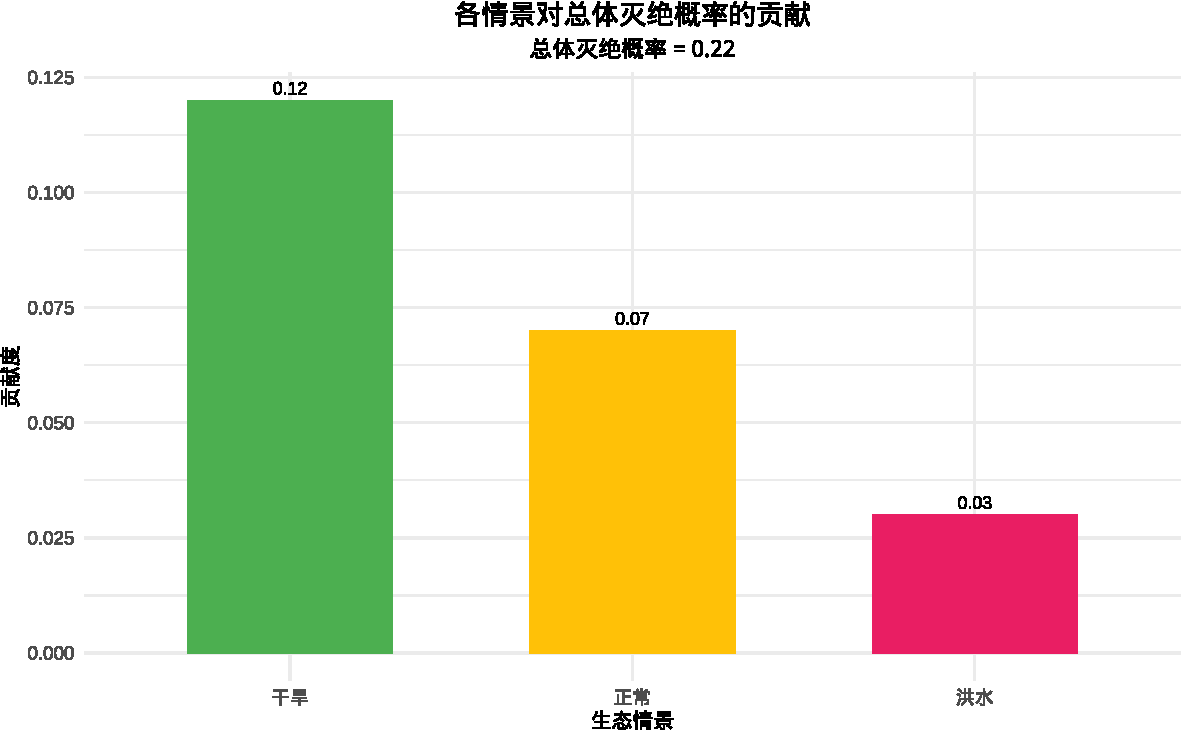
\includegraphics{02-probability_and_distribution_files/figure-latex/unnamed-chunk-4-1.pdf}

\textbf{在贝叶斯定理中的应用}:
在贝叶斯定理中,\(P(E)\)可以通过全概率公式计算:
\[P(E) = P(E|H) \times P(H) + P(E|\neg H) \times P(\neg H)\]
其中符号\(\neg H\)表示''假设H不成立'',即事件H的补集。

这就得到了贝叶斯定理的完整形式:
\[P(H|E) = \frac{P(E|H) \times P(H)}{P(E|H) \times P(H) + P(E|\neg H) \times P(\neg H)}\]

\textbf{贝叶斯概率的哲学基础}

贝叶斯概率体现了''学习''的本质。我们不是从零开始认识世界,而是基于已有的知识(先验),结合新的观察(证据),不断更新我们的认知(后验)。这种思维方式更接近人类实际的认知过程。

\textbf{贝叶斯概率的现实类比}

就像医学诊断:医生基于患者的症状(证据)更新对疾病的判断(假设)。

就像法庭审判:陪审团基于证据不断更新对被告有罪或无罪的信念。

就像天气预报:气象学家基于新的气象数据更新对天气变化的预测。

贝叶斯概率让我们从''静态世界''走向''动态世界'',用不断更新的信念来应对变化的环境。

\hypertarget{ux5b9aux4e49ux4e0eux8ba1ux7b97ux65b9ux6cd5-1}{%
\subsubsection{定义与计算方法}\label{ux5b9aux4e49ux4e0eux8ba1ux7b97ux65b9ux6cd5-1}}

贝叶斯概率的核心是贝叶斯定理,它提供了一个系统的方法来更新概率估计。通过全概率公式,我们得到了贝叶斯定理的完整形式,它考虑了所有可能的情况,确保概率的归一化。

\textbf{贝叶斯更新的步骤}

\begin{enumerate}
\def\labelenumi{\arabic{enumi}.}
\item
  \textbf{确定先验概率}:基于已有知识或经验,确定对假设的初始信念\(P(H)\)。
\item
  \textbf{计算似然函数}:评估在假设成立时观察到证据的概率\(P(E|H)\)。
\item
  \textbf{计算证据概率}:计算观察到证据的总体概率\(P(E)\)。
\item
  \textbf{计算后验概率}:使用贝叶斯定理更新信念,得到\(P(H|E)\)。
\end{enumerate}

\textbf{先验概率的选择}

在贝叶斯分析中,先验概率的选择很重要。常用的先验包括:
- \textbf{无信息先验}:当缺乏先验知识时使用
- \textbf{共轭先验}:数学上方便计算的后验分布
- \textbf{经验先验}:基于历史数据或专家意见

\textbf{贝叶斯定理基础演示}

\begin{Shaded}
\begin{Highlighting}[]
\CommentTok{\# 贝叶斯定理基础演示}
\FunctionTok{set.seed}\NormalTok{(}\DecValTok{1111}\NormalTok{)}

\CommentTok{\# 先验概率:疾病在种群中的 prevalence}
\NormalTok{prior\_prob }\OtherTok{\textless{}{-}} \FloatTok{0.05}  \CommentTok{\# 5\%的个体患病}

\CommentTok{\# 检测准确性}
\NormalTok{sensitivity }\OtherTok{\textless{}{-}} \FloatTok{0.95}  \CommentTok{\# 真阳性率}
\NormalTok{specificity }\OtherTok{\textless{}{-}} \FloatTok{0.90}  \CommentTok{\# 真阴性率}

\CommentTok{\# 计算边际概率: P(阳性)}
\NormalTok{marginal\_positive }\OtherTok{\textless{}{-}}\NormalTok{ prior\_prob }\SpecialCharTok{*}\NormalTok{ sensitivity }\SpecialCharTok{+}\NormalTok{ (}\DecValTok{1} \SpecialCharTok{{-}}\NormalTok{ prior\_prob) }\SpecialCharTok{*}\NormalTok{ (}\DecValTok{1} \SpecialCharTok{{-}}\NormalTok{ specificity)}

\CommentTok{\# 使用贝叶斯定理计算后验概率: P(患病|阳性)}
\NormalTok{posterior\_prob }\OtherTok{\textless{}{-}}\NormalTok{ (sensitivity }\SpecialCharTok{*}\NormalTok{ prior\_prob) }\SpecialCharTok{/}\NormalTok{ marginal\_positive}

\FunctionTok{cat}\NormalTok{(}\StringTok{"贝叶斯定理基础演示(疾病检测):}\SpecialCharTok{\textbackslash{}n}\StringTok{"}\NormalTok{)}
\end{Highlighting}
\end{Shaded}

\begin{verbatim}
## 贝叶斯定理基础演示(疾病检测):
\end{verbatim}

\begin{Shaded}
\begin{Highlighting}[]
\FunctionTok{cat}\NormalTok{(}\StringTok{"先验概率 P(患病):"}\NormalTok{, prior\_prob, }\StringTok{"}\SpecialCharTok{\textbackslash{}n}\StringTok{"}\NormalTok{)}
\end{Highlighting}
\end{Shaded}

\begin{verbatim}
## 先验概率 P(患病): 0.05
\end{verbatim}

\begin{Shaded}
\begin{Highlighting}[]
\FunctionTok{cat}\NormalTok{(}\StringTok{"检测灵敏度 P(阳性|患病):"}\NormalTok{, sensitivity, }\StringTok{"}\SpecialCharTok{\textbackslash{}n}\StringTok{"}\NormalTok{)}
\end{Highlighting}
\end{Shaded}

\begin{verbatim}
## 检测灵敏度 P(阳性|患病): 0.95
\end{verbatim}

\begin{Shaded}
\begin{Highlighting}[]
\FunctionTok{cat}\NormalTok{(}\StringTok{"检测特异度 P(阴性|健康):"}\NormalTok{, specificity, }\StringTok{"}\SpecialCharTok{\textbackslash{}n}\StringTok{"}\NormalTok{)}
\end{Highlighting}
\end{Shaded}

\begin{verbatim}
## 检测特异度 P(阴性|健康): 0.9
\end{verbatim}

\begin{Shaded}
\begin{Highlighting}[]
\FunctionTok{cat}\NormalTok{(}\StringTok{"边际概率 P(阳性):"}\NormalTok{, }\FunctionTok{round}\NormalTok{(marginal\_positive, }\DecValTok{4}\NormalTok{), }\StringTok{"}\SpecialCharTok{\textbackslash{}n}\StringTok{"}\NormalTok{)}
\end{Highlighting}
\end{Shaded}

\begin{verbatim}
## 边际概率 P(阳性): 0.1425
\end{verbatim}

\begin{Shaded}
\begin{Highlighting}[]
\FunctionTok{cat}\NormalTok{(}\StringTok{"后验概率 P(患病|阳性):"}\NormalTok{, }\FunctionTok{round}\NormalTok{(posterior\_prob, }\DecValTok{4}\NormalTok{), }\StringTok{"}\SpecialCharTok{\textbackslash{}n}\StringTok{"}\NormalTok{)}
\end{Highlighting}
\end{Shaded}

\begin{verbatim}
## 后验概率 P(患病|阳性): 0.3333
\end{verbatim}

\hypertarget{ux751fux6001ux5b66ux4e2dux7684ux8d1dux53f6ux65afux6982ux7387ux5e94ux7528}{%
\subsubsection{生态学中的贝叶斯概率应用}\label{ux751fux6001ux5b66ux4e2dux7684ux8d1dux53f6ux65afux6982ux7387ux5e94ux7528}}

贝叶斯概率在现代生态学研究中越来越重要:

\textbf{1. 物种分布模型}

结合专家知识和观测数据,建立更准确的物种分布预测模型。先验可以反映物种的生态习性,后验则结合了实际的分布数据。

贝叶斯方法在物种分布建模中具有独特优势,能够结合专家知识和观测数据:

\begin{Shaded}
\begin{Highlighting}[]
\CommentTok{\# 贝叶斯物种分布模型}
\FunctionTok{set.seed}\NormalTok{(}\DecValTok{1414}\NormalTok{)}

\CommentTok{\# 先验信息:专家对物种偏好的信念}
\NormalTok{expert\_prior }\OtherTok{\textless{}{-}} \FunctionTok{c}\NormalTok{(}\FloatTok{0.6}\NormalTok{, }\FloatTok{0.3}\NormalTok{, }\FloatTok{0.1}\NormalTok{)  }\CommentTok{\# 喜欢森林、草地、湿地的先验概率}
\NormalTok{habitat\_types }\OtherTok{\textless{}{-}} \FunctionTok{c}\NormalTok{(}\StringTok{"森林"}\NormalTok{, }\StringTok{"草地"}\NormalTok{, }\StringTok{"湿地"}\NormalTok{)}

\CommentTok{\# 观测数据:在不同栖息地中发现物种的次数}
\NormalTok{observations }\OtherTok{\textless{}{-}} \FunctionTok{c}\NormalTok{(}\DecValTok{45}\NormalTok{, }\DecValTok{20}\NormalTok{, }\DecValTok{5}\NormalTok{)      }\CommentTok{\# 在森林、草地、湿地中的观测次数}
\NormalTok{total\_observations }\OtherTok{\textless{}{-}} \FunctionTok{sum}\NormalTok{(observations)}

\CommentTok{\# 计算似然函数(基于观测数据)}
\NormalTok{likelihood }\OtherTok{\textless{}{-}}\NormalTok{ observations }\SpecialCharTok{/}\NormalTok{ total\_observations}

\CommentTok{\# 计算证据概率}
\NormalTok{evidence }\OtherTok{\textless{}{-}} \FunctionTok{sum}\NormalTok{(expert\_prior }\SpecialCharTok{*}\NormalTok{ likelihood)}

\CommentTok{\# 贝叶斯更新}
\NormalTok{posterior }\OtherTok{\textless{}{-}}\NormalTok{ (expert\_prior }\SpecialCharTok{*}\NormalTok{ likelihood) }\SpecialCharTok{/}\NormalTok{ evidence}

\CommentTok{\# 结果分析}
\NormalTok{results }\OtherTok{\textless{}{-}} \FunctionTok{data.frame}\NormalTok{(}
\NormalTok{  栖息地类型 }\OtherTok{=}\NormalTok{ habitat\_types,}
\NormalTok{  专家先验 }\OtherTok{=} \FunctionTok{round}\NormalTok{(expert\_prior, }\DecValTok{3}\NormalTok{),}
\NormalTok{  观测似然 }\OtherTok{=} \FunctionTok{round}\NormalTok{(likelihood, }\DecValTok{3}\NormalTok{),}
\NormalTok{  贝叶斯后验 }\OtherTok{=} \FunctionTok{round}\NormalTok{(posterior, }\DecValTok{3}\NormalTok{)}
\NormalTok{)}

\FunctionTok{cat}\NormalTok{(}\StringTok{"贝叶斯物种分布模型结果:}\SpecialCharTok{\textbackslash{}n}\StringTok{"}\NormalTok{)}
\end{Highlighting}
\end{Shaded}

\begin{verbatim}
## 贝叶斯物种分布模型结果:
\end{verbatim}

\begin{Shaded}
\begin{Highlighting}[]
\FunctionTok{print}\NormalTok{(results)}
\end{Highlighting}
\end{Shaded}

\begin{verbatim}
##   栖息地类型 专家先验 观测似然 贝叶斯后验
## 1       森林      0.6    0.643      0.806
## 2       草地      0.3    0.286      0.179
## 3       湿地      0.1    0.071      0.015
\end{verbatim}

\begin{Shaded}
\begin{Highlighting}[]
\CommentTok{\# 计算信息增益(KL散度)}
\NormalTok{kl\_divergence }\OtherTok{\textless{}{-}} \FunctionTok{sum}\NormalTok{(posterior }\SpecialCharTok{*} \FunctionTok{log}\NormalTok{(posterior }\SpecialCharTok{/}\NormalTok{ expert\_prior))}
\FunctionTok{cat}\NormalTok{(}\StringTok{"KL散度(信息增益):"}\NormalTok{, }\FunctionTok{round}\NormalTok{(kl\_divergence, }\DecValTok{4}\NormalTok{), }\StringTok{"}\SpecialCharTok{\textbackslash{}n}\StringTok{"}\NormalTok{)}
\end{Highlighting}
\end{Shaded}

\begin{verbatim}
## KL散度(信息增益): 0.1171
\end{verbatim}

\begin{Shaded}
\begin{Highlighting}[]
\CommentTok{\# 贝叶斯因子计算}
\NormalTok{bayes\_factor }\OtherTok{\textless{}{-}}\NormalTok{ (posterior[}\DecValTok{1}\NormalTok{] }\SpecialCharTok{/}\NormalTok{ (}\DecValTok{1} \SpecialCharTok{{-}}\NormalTok{ posterior[}\DecValTok{1}\NormalTok{])) }\SpecialCharTok{/}\NormalTok{ (expert\_prior[}\DecValTok{1}\NormalTok{] }\SpecialCharTok{/}\NormalTok{ (}\DecValTok{1} \SpecialCharTok{{-}}\NormalTok{ expert\_prior[}\DecValTok{1}\NormalTok{]))}
\FunctionTok{cat}\NormalTok{(}\StringTok{"贝叶斯因子(森林偏好):"}\NormalTok{, }\FunctionTok{round}\NormalTok{(bayes\_factor, }\DecValTok{2}\NormalTok{), }\StringTok{"}\SpecialCharTok{\textbackslash{}n}\StringTok{"}\NormalTok{)}
\end{Highlighting}
\end{Shaded}

\begin{verbatim}
## 贝叶斯因子(森林偏好): 2.77
\end{verbatim}

\begin{Shaded}
\begin{Highlighting}[]
\ControlFlowTok{if}\NormalTok{ (bayes\_factor }\SpecialCharTok{\textgreater{}} \DecValTok{3}\NormalTok{) \{}
  \FunctionTok{cat}\NormalTok{(}\StringTok{"强烈支持物种偏好森林的假设}\SpecialCharTok{\textbackslash{}n}\StringTok{"}\NormalTok{)}
\NormalTok{\} }\ControlFlowTok{else} \ControlFlowTok{if}\NormalTok{ (bayes\_factor }\SpecialCharTok{\textgreater{}} \DecValTok{1}\NormalTok{) \{}
  \FunctionTok{cat}\NormalTok{(}\StringTok{"微弱支持物种偏好森林的假设}\SpecialCharTok{\textbackslash{}n}\StringTok{"}\NormalTok{)}
\NormalTok{\} }\ControlFlowTok{else}\NormalTok{ \{}
  \FunctionTok{cat}\NormalTok{(}\StringTok{"证据不支持物种偏好森林的假设}\SpecialCharTok{\textbackslash{}n}\StringTok{"}\NormalTok{)}
\NormalTok{\}}
\end{Highlighting}
\end{Shaded}

\begin{verbatim}
## 微弱支持物种偏好森林的假设
\end{verbatim}

\textbf{2. 种群动态预测}

基于历史种群数据和环境变化信息,预测未来种群数量的变化趋势。贝叶斯方法能够处理参数的不确定性。

\textbf{3. 保护优先级评估}

结合多种证据(如栖息地质量、种群趋势、威胁因素)来评估物种的保护优先级。

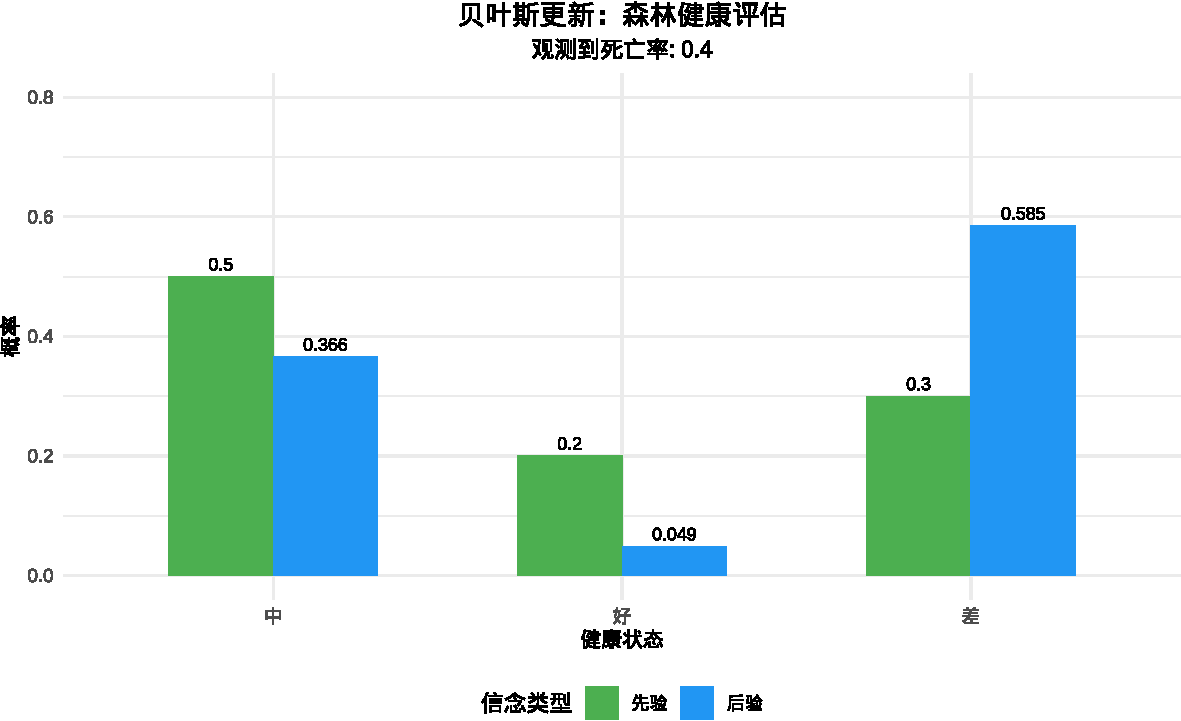
\includegraphics{02-probability_and_distribution_files/figure-latex/unnamed-chunk-7-1.pdf}

\textbf{4. 生态风险评估}

在数据有限的情况下,结合专家判断和有限观测来评估生态风险。

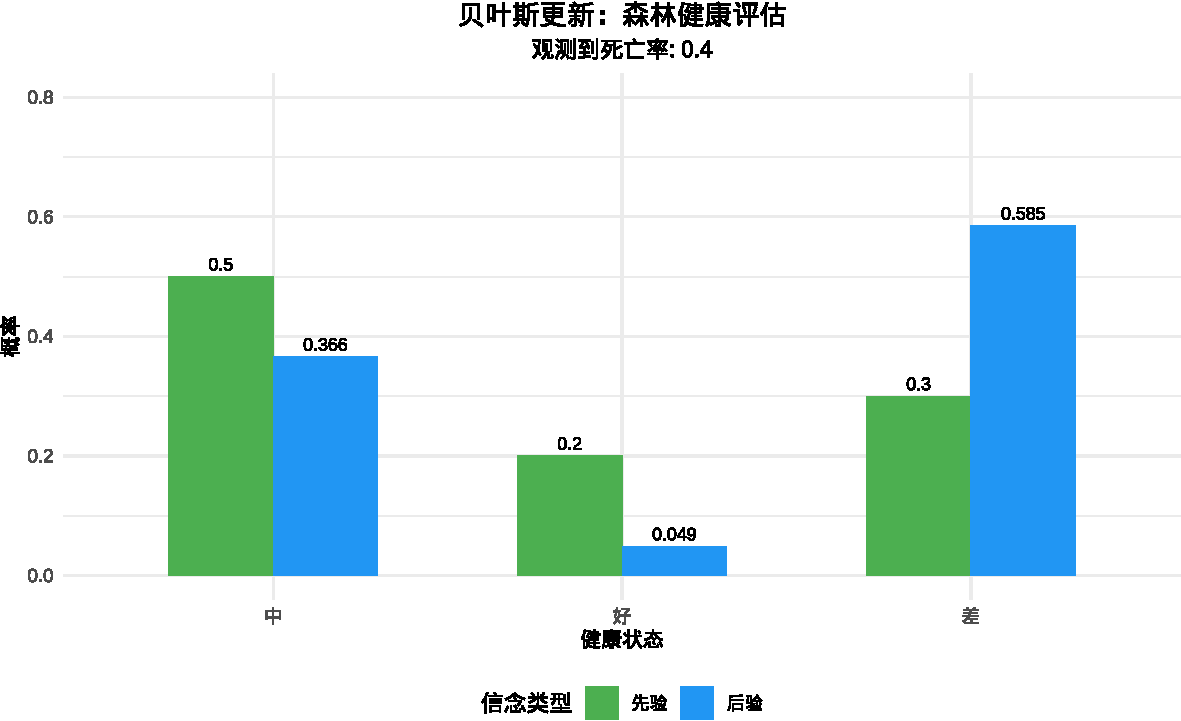
\includegraphics{02-probability_and_distribution_files/figure-latex/unnamed-chunk-8-1.pdf} 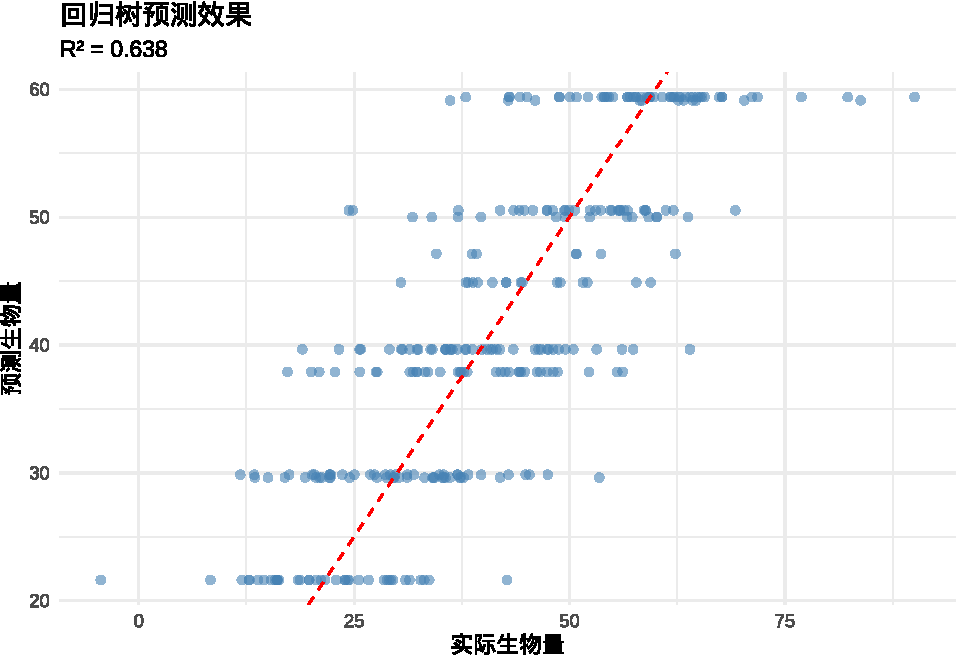
\includegraphics{02-probability_and_distribution_files/figure-latex/unnamed-chunk-8-2.pdf}

\textbf{5. 模型选择与平均}

使用贝叶斯模型平均方法,综合考虑多个竞争模型的预测结果。

\begin{verbatim}
## 贝叶斯模型比较结果:
\end{verbatim}

\begin{verbatim}
##       模型     模型证据 贝叶斯因子
## 1 线性模型 7.411531e-52       1.00
## 2 季节模型 1.036188e-47   13980.76
\end{verbatim}

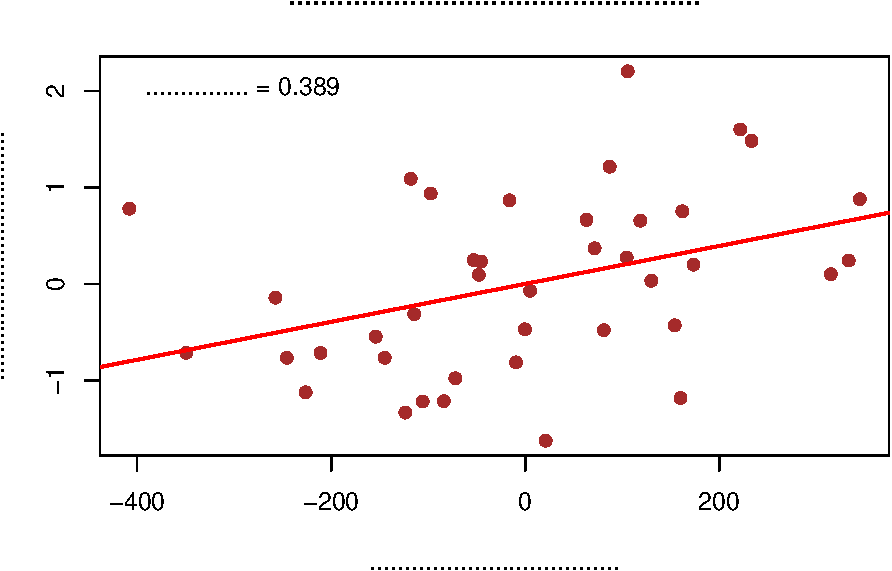
\includegraphics{02-probability_and_distribution_files/figure-latex/unnamed-chunk-9-1.pdf}

敏感性分析与稳健性检验

\begin{Shaded}
\begin{Highlighting}[]
\CommentTok{\# 贝叶斯敏感性分析}
\NormalTok{sensitivity\_analysis }\OtherTok{\textless{}{-}} \ControlFlowTok{function}\NormalTok{(prior\_strength) \{}
  \CommentTok{\# 不同先验强度下的后验分析}
  \FunctionTok{set.seed}\NormalTok{(}\DecValTok{1717}\NormalTok{)}

  \CommentTok{\# 生成生态数据}
\NormalTok{  true\_effect }\OtherTok{\textless{}{-}} \FloatTok{0.8}
\NormalTok{  observed\_data }\OtherTok{\textless{}{-}} \FunctionTok{rnorm}\NormalTok{(}\DecValTok{30}\NormalTok{, true\_effect, }\FloatTok{0.5}\NormalTok{)}

  \CommentTok{\# 不同先验强度}
\NormalTok{  prior\_sd }\OtherTok{\textless{}{-}} \DecValTok{10} \SpecialCharTok{/}\NormalTok{ prior\_strength  }\CommentTok{\# 先验标准差随强度变化}

  \CommentTok{\# 简单贝叶斯更新}
\NormalTok{  prior\_mean }\OtherTok{\textless{}{-}} \DecValTok{0}
\NormalTok{  sample\_mean }\OtherTok{\textless{}{-}} \FunctionTok{mean}\NormalTok{(observed\_data)}
\NormalTok{  sample\_sd }\OtherTok{\textless{}{-}} \FunctionTok{sd}\NormalTok{(observed\_data) }\SpecialCharTok{/} \FunctionTok{sqrt}\NormalTok{(}\FunctionTok{length}\NormalTok{(observed\_data))}

  \CommentTok{\# 后验计算(正态{-}正态共轭)}
\NormalTok{  posterior\_precision }\OtherTok{\textless{}{-}} \DecValTok{1}\SpecialCharTok{/}\NormalTok{prior\_sd}\SpecialCharTok{\^{}}\DecValTok{2} \SpecialCharTok{+} \DecValTok{1}\SpecialCharTok{/}\NormalTok{sample\_sd}\SpecialCharTok{\^{}}\DecValTok{2}
\NormalTok{  posterior\_mean }\OtherTok{\textless{}{-}}\NormalTok{ (prior\_mean}\SpecialCharTok{/}\NormalTok{prior\_sd}\SpecialCharTok{\^{}}\DecValTok{2} \SpecialCharTok{+}\NormalTok{ sample\_mean}\SpecialCharTok{/}\NormalTok{sample\_sd}\SpecialCharTok{\^{}}\DecValTok{2}\NormalTok{) }\SpecialCharTok{/}\NormalTok{ posterior\_precision}
\NormalTok{  posterior\_sd }\OtherTok{\textless{}{-}} \FunctionTok{sqrt}\NormalTok{(}\DecValTok{1} \SpecialCharTok{/}\NormalTok{ posterior\_precision)}

  \FunctionTok{return}\NormalTok{(}\FunctionTok{c}\NormalTok{(posterior\_mean, posterior\_sd))}
\NormalTok{\}}

\CommentTok{\# 测试不同先验强度}
\NormalTok{prior\_strengths }\OtherTok{\textless{}{-}} \FunctionTok{c}\NormalTok{(}\FloatTok{0.1}\NormalTok{, }\FloatTok{0.5}\NormalTok{, }\DecValTok{1}\NormalTok{, }\DecValTok{2}\NormalTok{, }\DecValTok{5}\NormalTok{, }\DecValTok{10}\NormalTok{)}
\NormalTok{sensitivity\_results }\OtherTok{\textless{}{-}} \FunctionTok{t}\NormalTok{(}\FunctionTok{sapply}\NormalTok{(prior\_strengths, sensitivity\_analysis))}

\NormalTok{sensitivity\_df }\OtherTok{\textless{}{-}} \FunctionTok{data.frame}\NormalTok{(}
\NormalTok{  先验强度 }\OtherTok{=}\NormalTok{ prior\_strengths,}
\NormalTok{  后验均值 }\OtherTok{=} \FunctionTok{round}\NormalTok{(sensitivity\_results[,}\DecValTok{1}\NormalTok{], }\DecValTok{3}\NormalTok{),}
\NormalTok{  后验标准差 }\OtherTok{=} \FunctionTok{round}\NormalTok{(sensitivity\_results[,}\DecValTok{2}\NormalTok{], }\DecValTok{3}\NormalTok{)}
\NormalTok{)}

\FunctionTok{cat}\NormalTok{(}\StringTok{"贝叶斯敏感性分析结果:}\SpecialCharTok{\textbackslash{}n}\StringTok{"}\NormalTok{)}
\end{Highlighting}
\end{Shaded}

\begin{verbatim}
## 贝叶斯敏感性分析结果:
\end{verbatim}

\begin{Shaded}
\begin{Highlighting}[]
\FunctionTok{print}\NormalTok{(sensitivity\_df)}
\end{Highlighting}
\end{Shaded}

\begin{verbatim}
##   先验强度 后验均值 后验标准差
## 1      0.1    0.708      0.097
## 2      0.5    0.708      0.097
## 3      1.0    0.708      0.097
## 4      2.0    0.708      0.097
## 5      5.0    0.706      0.097
## 6     10.0    0.702      0.096
\end{verbatim}

\begin{Shaded}
\begin{Highlighting}[]
\CommentTok{\# 稳健性检验}
\NormalTok{robustness\_check }\OtherTok{\textless{}{-}} \ControlFlowTok{function}\NormalTok{(data\_contamination) \{}
  \CommentTok{\# 检验数据污染对结果的影响}
  \FunctionTok{set.seed}\NormalTok{(}\DecValTok{1818}\NormalTok{)}

  \CommentTok{\# 生成清洁数据}
\NormalTok{  clean\_data }\OtherTok{\textless{}{-}} \FunctionTok{rnorm}\NormalTok{(}\DecValTok{25}\NormalTok{, }\FloatTok{0.5}\NormalTok{, }\FloatTok{0.3}\NormalTok{)}

  \CommentTok{\# 添加污染数据}
\NormalTok{  n\_contaminated }\OtherTok{\textless{}{-}} \FunctionTok{round}\NormalTok{(}\FunctionTok{length}\NormalTok{(clean\_data) }\SpecialCharTok{*}\NormalTok{ data\_contamination)}
  \ControlFlowTok{if}\NormalTok{ (n\_contaminated }\SpecialCharTok{\textgreater{}} \DecValTok{0}\NormalTok{) \{}
\NormalTok{    contaminated\_data }\OtherTok{\textless{}{-}} \FunctionTok{rnorm}\NormalTok{(n\_contaminated, }\FloatTok{2.0}\NormalTok{, }\FloatTok{0.5}\NormalTok{)  }\CommentTok{\# 异常值}
\NormalTok{    all\_data }\OtherTok{\textless{}{-}} \FunctionTok{c}\NormalTok{(clean\_data, contaminated\_data)}
\NormalTok{  \} }\ControlFlowTok{else}\NormalTok{ \{}
\NormalTok{    all\_data }\OtherTok{\textless{}{-}}\NormalTok{ clean\_data}
\NormalTok{  \}}

  \CommentTok{\# 贝叶斯分析}
\NormalTok{  prior\_mean }\OtherTok{\textless{}{-}} \DecValTok{0}
\NormalTok{  prior\_sd }\OtherTok{\textless{}{-}} \DecValTok{1}

\NormalTok{  sample\_mean }\OtherTok{\textless{}{-}} \FunctionTok{mean}\NormalTok{(all\_data)}
\NormalTok{  sample\_sd }\OtherTok{\textless{}{-}} \FunctionTok{sd}\NormalTok{(all\_data) }\SpecialCharTok{/} \FunctionTok{sqrt}\NormalTok{(}\FunctionTok{length}\NormalTok{(all\_data))}

\NormalTok{  posterior\_precision }\OtherTok{\textless{}{-}} \DecValTok{1}\SpecialCharTok{/}\NormalTok{prior\_sd}\SpecialCharTok{\^{}}\DecValTok{2} \SpecialCharTok{+} \DecValTok{1}\SpecialCharTok{/}\NormalTok{sample\_sd}\SpecialCharTok{\^{}}\DecValTok{2}
\NormalTok{  posterior\_mean }\OtherTok{\textless{}{-}}\NormalTok{ (prior\_mean}\SpecialCharTok{/}\NormalTok{prior\_sd}\SpecialCharTok{\^{}}\DecValTok{2} \SpecialCharTok{+}\NormalTok{ sample\_mean}\SpecialCharTok{/}\NormalTok{sample\_sd}\SpecialCharTok{\^{}}\DecValTok{2}\NormalTok{) }\SpecialCharTok{/}\NormalTok{ posterior\_precision}

  \FunctionTok{return}\NormalTok{(posterior\_mean)}
\NormalTok{\}}

\CommentTok{\# 测试不同污染水平}
\NormalTok{contamination\_levels }\OtherTok{\textless{}{-}} \FunctionTok{c}\NormalTok{(}\DecValTok{0}\NormalTok{, }\FloatTok{0.05}\NormalTok{, }\FloatTok{0.1}\NormalTok{, }\FloatTok{0.2}\NormalTok{, }\FloatTok{0.3}\NormalTok{)}
\NormalTok{robustness\_results }\OtherTok{\textless{}{-}} \FunctionTok{sapply}\NormalTok{(contamination\_levels, robustness\_check)}

\NormalTok{robustness\_df }\OtherTok{\textless{}{-}} \FunctionTok{data.frame}\NormalTok{(}
\NormalTok{  污染比例 }\OtherTok{=}\NormalTok{ contamination\_levels,}
\NormalTok{  后验均值 }\OtherTok{=} \FunctionTok{round}\NormalTok{(robustness\_results, }\DecValTok{3}\NormalTok{)}
\NormalTok{)}

\FunctionTok{cat}\NormalTok{(}\StringTok{"}\SpecialCharTok{\textbackslash{}n}\StringTok{贝叶斯稳健性检验结果:}\SpecialCharTok{\textbackslash{}n}\StringTok{"}\NormalTok{)}
\end{Highlighting}
\end{Shaded}

\begin{verbatim}
## 
## 贝叶斯稳健性检验结果:
\end{verbatim}

\begin{Shaded}
\begin{Highlighting}[]
\FunctionTok{print}\NormalTok{(robustness\_df)}
\end{Highlighting}
\end{Shaded}

\begin{verbatim}
##   污染比例 后验均值
## 1     0.00    0.539
## 2     0.05    0.604
## 3     0.10    0.683
## 4     0.20    0.804
## 5     0.30    0.888
\end{verbatim}

\hypertarget{ux8d1dux53f6ux65afux6982ux7387ux7684ux4f18ux52bfux4e0eux5c40ux9650ux6027}{%
\subsubsection{贝叶斯概率的优势与局限性}\label{ux8d1dux53f6ux65afux6982ux7387ux7684ux4f18ux52bfux4e0eux5c40ux9650ux6027}}

贝叶斯概率方法在现代生态学研究中展现出独特的优势。其\textbf{灵活性}体现在能够有机地结合先验知识和新的观测证据,这种动态更新的特性使其特别适合处理环境变化和物种适应性研究。通过贝叶斯定理,研究者可以将专家经验、历史数据与最新的实地观察相结合,形成更加全面的认知。\textbf{不确定性量化}是贝叶斯方法的另一重要优势,它不仅提供点估计,还能明确表达参数的不确定性范围,这对于生态风险评估和保护决策具有重要意义。在\textbf{小样本适用性}方面,贝叶斯方法在数据有限的情况下仍然能够发挥作用,这对于研究稀有物种或难以大规模观察的生态现象尤为宝贵。\textbf{模型复杂性处理}能力使贝叶斯方法能够应对生态学中常见的多层次、多变量复杂系统,如考虑个体差异、空间异质性和时间动态的生态模型。最重要的是,贝叶斯方法提供\textbf{决策支持},直接输出决策所需的概率信息,如物种灭绝风险、保护措施效果等,为生态管理提供科学依据。

然而,贝叶斯概率方法也存在不容忽视的局限性。\textbf{主观性}是其最受争议的方面,先验概率的选择往往依赖于研究者的主观判断,不同专家可能会给出不同的先验设定。\textbf{计算复杂性}是实际应用中的主要障碍,复杂的贝叶斯模型需要大量的计算资源,特别是使用马尔可夫链蒙特卡洛方法时,计算时间可能相当可观。\textbf{先验敏感性}问题意味着结果可能对先验选择高度敏感,不恰当的先验设定可能导致有偏的结论。\textbf{收敛问题}是MCMC方法特有的挑战,在复杂模型中可能出现收敛困难或收敛到局部最优解的情况。此外,\textbf{解释难度}限制了贝叶斯方法的普及,后验分布的理解和解释需要研究者具备相当的统计背景,这在一定程度上阻碍了其在生态学实践中的广泛应用。这些局限性提示我们在使用贝叶斯方法时需要谨慎处理先验设定,并充分考虑计算可行性和结果解释的清晰性。

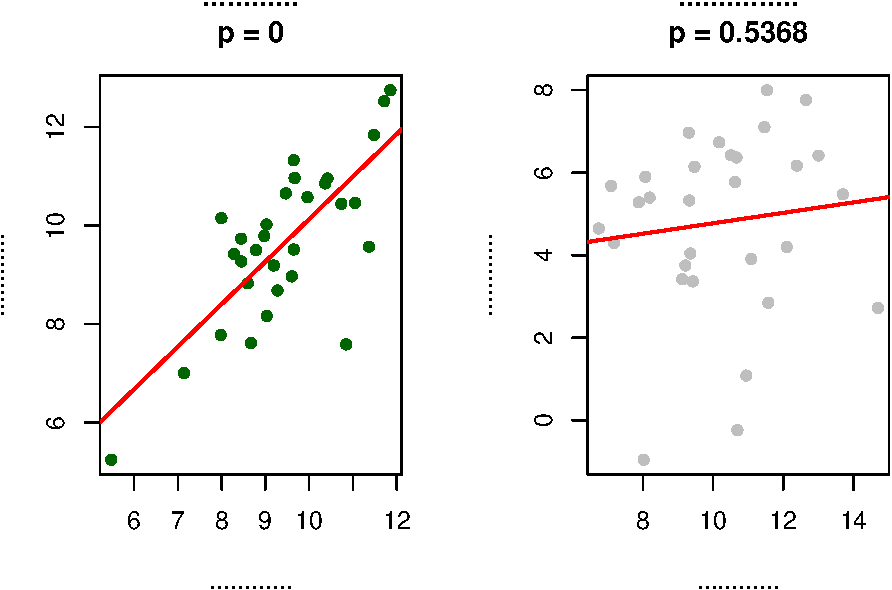
\includegraphics{02-probability_and_distribution_files/figure-latex/unnamed-chunk-11-1.pdf}

\hypertarget{ux8d1dux53f6ux65afux7edfux8ba1ux7684ux6311ux6218ux53caux89e3ux51b3ux65b9ux6848}{%
\subsubsection{贝叶斯统计的挑战及解决方案}\label{ux8d1dux53f6ux65afux7edfux8ba1ux7684ux6311ux6218ux53caux89e3ux51b3ux65b9ux6848}}

贝叶斯框架在概念上非常优雅,但在计算上有一个巨大的挑战:\textbf{分母 \(P(E)\) 通常极其难以计算。}

\[ P(E) = \int P(E \mid \theta) P(\theta) \, d\theta \]

这个积分在高维空间(即参数\(\theta\)包含多个变量时)往往没有解析解(即无法用公式直接写出结果)。这严重限制了贝叶斯方法的应用,人们只能对那些具有``共轭先验''的特殊模型进行分析(即先验和后验属于同一分布家族,从而可以避开积分计算)。

\textbf{所以,问题的核心变成了:如何有效地从复杂的、高维的后验分布 \(P(\theta \mid E)\) 中获取信息(例如,计算均值、方差、分位数等),而无需知道那个讨厌的分母 \(P(E)\)?}

\textbf{马尔可夫模拟(MCMC)的核心思想}

MCMC是一类算法的总称,它巧妙地解决了上述挑战。它的核心思想是:

\textbf{与其直接计算后验分布,不如我们构造一个马尔可夫链,使其平稳分布恰好就是我们想要的后验分布 \(P(\theta \mid E)\)。然后,我们从这个链中生成大量的样本,用这些样本来近似(模拟)后验分布。}

想象一下,你是一个盲人,想要了解一头大象的形状。这头大象就是贝叶斯统计中的\textbf{后验分布}------我们想要了解但无法直接看到的复杂概率分布。

\textbf{贝叶斯的难题}:大象的形状太复杂了,你无法用数学公式精确描述它(就像无法直接计算分母P(E)一样)。

\textbf{MCMC的解决方案}:你不需要知道大象的精确形状,只需要通过''触摸''来了解它:

\begin{enumerate}
\def\labelenumi{\arabic{enumi}.}
\item
  \textbf{马尔可夫链}:你开始在大象周围随机走动,但遵循一个聪明的规则------每次移动时,你更倾向于走向大象''更胖''的区域(高概率区域),而不是''更瘦''的区域(低概率区域)。
\item
  \textbf{蒙特卡洛抽样}:你边走边触摸大象,记录下每个位置的感受。虽然每次触摸只能了解一小部分,但经过成千上万次触摸后,你就能在心中构建出大象的整体形状。
\item
  \textbf{巧妙之处}:你根本不需要知道大象的确切形状!你只需要比较当前位置和下一个位置哪个''更胖''(通过概率比值),这个比值中讨厌的分母P(E)会自动抵消掉。
\end{enumerate}

\textbf{结果}:经过足够多的''触摸''后,你收集到的位置样本就精确地反映了大象的真实形状。你可以通过这些样本计算大象的平均高度(后验均值)、宽度(后验方差),甚至画出大象的轮廓(后验分布图)。

就像盲人通过系统性的触摸来了解复杂的大象形状一样,MCMC通过系统性的随机游走来探索复杂的生态学后验分布,让我们能够在不知道精确数学解的情况下,仍然能够对生态系统的参数做出可靠的贝叶斯推断。

我们来用正式的语言分解MCMC这个思想:

\begin{enumerate}
\def\labelenumi{\arabic{enumi}.}
\item
  \textbf{蒙特卡洛(Monte Carlo)}: 泛指通过随机抽样来解决问题的方法。基本思想是:如果你想知道一个分布的属性(比如均值),就从该分布中抽取大量样本,然后计算这些样本的均值。\textbf{问题在于}:我们无法直接从复杂的后验分布中抽样。
\item
  \textbf{马尔可夫链(Markov Chain)}: 这是一个具有``无记忆''性质的随机过程,下一个状态只取决于当前状态,而与过去的状态无关。关键点是,在满足一定条件下,马尔可夫链会收敛到一个唯一的\textbf{平稳分布}。这意味着无论链从何处开始,经过足够长的步骤后,它停留在每个状态的概率是固定的。
\item
  \textbf{MCMC的巧妙结合}:

  \begin{itemize}
  \tightlist
  \item
    \textbf{目标}: 让后验分布 \(P(\theta \mid E)\) 成为马尔可夫链的平稳分布。
  \item
    \textbf{方法}: 设计特定的规则(如Metropolis-Hastings算法或Gibbs抽样),来构建这样一个链。这些规则的伟大之处在于,它们在计算时,\textbf{分母 \(P(E)\) 会被约掉!} 因为规则中只涉及后验分布的\emph{比值}:
    \[ \frac{P(\theta_{\text{新}} \mid E)}{P(\theta_{\text{旧}} \mid E)} = \frac{\frac{P(E \mid \theta_{\text{新}})P(\theta_{\text{新}})}{P(E)}}{\frac{P(E \mid \theta_{\text{旧}})P(\theta_{\text{旧}})}{P(E)}} = \frac{P(E \mid \theta_{\text{新}})P(\theta_{\text{新}})}{P(E \mid \theta_{\text{旧}})P(\theta_{\text{旧}})} \]
    \(P(E)\) 被完美地消去了。所以我们可以在完全不知道 \(P(E)\) 的情况下,判断是否应该从当前参数 \(\theta_{\text{旧}}\) 移动到新参数 \(\theta_{\text{新}}\)。
  \item
    \textbf{过程}: 算法从某个初始值开始,然后根据规则随机游走。经过一段''预烧期''后,链会收敛到平稳分布。之后产生的样本,虽然彼此相关(因为是马尔可夫链),但可以看作是来自后验分布 \(P(\theta \mid E)\) 的(近似)样本。
  \end{itemize}
\end{enumerate}

\textbf{两者的关系------完美的共生}

现在我们可以清晰地描述它们的关系:

\begin{enumerate}
\def\labelenumi{\arabic{enumi}.}
\item
  \textbf{目标与手段的关系}:

  \begin{itemize}
  \tightlist
  \item
    \textbf{贝叶斯统计是目标}: 它定义了我们要解决的问题------求得后验分布。
  \item
    \textbf{MCMC是手段}: 它提供了实现这个目标的计算引擎。没有MCMC,贝叶斯理论对于许多复杂模型只能是``纸上谈兵''。
  \end{itemize}
\item
  \textbf{计算上的突破}:
  MCMC的出现(特别是在1990年代以后)是贝叶斯统计复兴和广泛应用的根本原因。它使得分析者可以自由地构建复杂的、非共轭的、高维的模型,而无需担心无法计算的积分。几乎所有现代的贝叶斯软件(如Stan, PyMC, JAGS)的核心都是MCMC算法。
\item
  \textbf{工作流程示例}:
  一个典型的贝叶斯数据分析流程如下:

  \begin{itemize}
  \tightlist
  \item
    \textbf{步骤1(贝叶斯)}: 建立模型。设定似然函数 \(P(E \mid \theta)\) 和先验分布 \(P(\theta)\)。
  \item
    \textbf{步骤2(MCMC)}: 计算后验。使用MCMC算法(如Metropolis-Hastings, Gibbs抽样, Hamiltonian Monte Carlo)从后验分布 \(P(\theta \mid E)\) 中生成大量样本 \(\theta^{(1)}, \theta^{(2)}, ..., \theta^{(N)}\)。
  \item
    \textbf{步骤3(贝叶斯+蒙特卡洛)}: 后验推断。利用生成的样本进行蒙特卡洛积分:

    \begin{itemize}
    \tightlist
    \item
      后验均值: \(E[\theta \mid E] \approx \frac{1}{N} \sum_{i=1}^N \theta^{(i)}\)
    \item
      后验区间: 使用样本的分位数来构造可信区间。
    \item
      后验预测: 也可以轻松生成对新数据的预测。
    \end{itemize}
  \end{itemize}
\end{enumerate}

\textbf{小结}

\begin{longtable}[]{@{}
  >{\raggedright\arraybackslash}p{(\columnwidth - 4\tabcolsep) * \real{0.3333}}
  >{\raggedright\arraybackslash}p{(\columnwidth - 4\tabcolsep) * \real{0.3333}}
  >{\raggedright\arraybackslash}p{(\columnwidth - 4\tabcolsep) * \real{0.3333}}@{}}
\toprule\noalign{}
\begin{minipage}[b]{\linewidth}\raggedright
特性
\end{minipage} & \begin{minipage}[b]{\linewidth}\raggedright
贝叶斯统计
\end{minipage} & \begin{minipage}[b]{\linewidth}\raggedright
马尔可夫链蒙特卡洛(MCMC)
\end{minipage} \\
\midrule\noalign{}
\endhead
\bottomrule\noalign{}
\endlastfoot
\textbf{本质} & \textbf{推理框架} & \textbf{计算方法} \\
\textbf{核心} & 使用贝叶斯定理将先验信念和数据进行结合,更新为后验信念。 & 通过构造一个平稳分布为目标分布的马尔可夫链来进行抽样。 \\
\textbf{角色} & 提出``要计算什么''(后验分布)。 & 解决``如何计算''的问题。 \\
\textbf{依赖关系} & 理论上不依赖MCMC(例如,可使用共轭先验或变分推断)。 & 通常为贝叶斯计算服务,但其思想也可用于其他领域(如统计物理、优化)。 \\
\end{longtable}

\textbf{结论就是:贝叶斯统计为概率建模提供了哲学和理论基础,而马尔可夫模拟(MCMC)则提供了使这个理论在实践中得以实现的强大计算工具。两者相辅相成,共同推动了现代统计学、机器学习和数据科学的发展。}

\hypertarget{ux7b80ux5355mcmcux6f14ux793a}{%
\subsubsection{简单MCMC演示}\label{ux7b80ux5355mcmcux6f14ux793a}}

马尔可夫链蒙特卡洛(MCMC)方法是贝叶斯计算的核心工具:

\begin{Shaded}
\begin{Highlighting}[]
\CommentTok{\# 简单MCMC采样演示}
\NormalTok{simple\_mcmc }\OtherTok{\textless{}{-}} \ControlFlowTok{function}\NormalTok{(n\_iterations, prior\_mean, prior\_sd, data, likelihood\_sd) \{}
  \CommentTok{\# 初始化}
\NormalTok{  current\_value }\OtherTok{\textless{}{-}}\NormalTok{ prior\_mean}
\NormalTok{  samples }\OtherTok{\textless{}{-}} \FunctionTok{numeric}\NormalTok{(n\_iterations)}
\NormalTok{  accepts }\OtherTok{\textless{}{-}} \DecValTok{0}

  \ControlFlowTok{for}\NormalTok{ (i }\ControlFlowTok{in} \DecValTok{1}\SpecialCharTok{:}\NormalTok{n\_iterations) \{}
    \CommentTok{\# 建议新值}
\NormalTok{    proposal }\OtherTok{\textless{}{-}} \FunctionTok{rnorm}\NormalTok{(}\DecValTok{1}\NormalTok{, current\_value, }\FloatTok{0.1}\NormalTok{)}

    \CommentTok{\# 计算先验概率}
\NormalTok{    prior\_current }\OtherTok{\textless{}{-}} \FunctionTok{dnorm}\NormalTok{(current\_value, prior\_mean, prior\_sd)}
\NormalTok{    prior\_proposal }\OtherTok{\textless{}{-}} \FunctionTok{dnorm}\NormalTok{(proposal, prior\_mean, prior\_sd)}

    \CommentTok{\# 计算似然概率}
\NormalTok{    likelihood\_current }\OtherTok{\textless{}{-}} \FunctionTok{prod}\NormalTok{(}\FunctionTok{dnorm}\NormalTok{(data, current\_value, likelihood\_sd))}
\NormalTok{    likelihood\_proposal }\OtherTok{\textless{}{-}} \FunctionTok{prod}\NormalTok{(}\FunctionTok{dnorm}\NormalTok{(data, proposal, likelihood\_sd))}

    \CommentTok{\# 计算接受概率}
\NormalTok{    acceptance\_ratio }\OtherTok{\textless{}{-}}\NormalTok{ (prior\_proposal }\SpecialCharTok{*}\NormalTok{ likelihood\_proposal) }\SpecialCharTok{/}\NormalTok{ (prior\_current }\SpecialCharTok{*}\NormalTok{ likelihood\_current)}
\NormalTok{    acceptance\_prob }\OtherTok{\textless{}{-}} \FunctionTok{min}\NormalTok{(}\DecValTok{1}\NormalTok{, acceptance\_ratio)}

    \CommentTok{\# 决定是否接受}
    \ControlFlowTok{if}\NormalTok{ (}\FunctionTok{runif}\NormalTok{(}\DecValTok{1}\NormalTok{) }\SpecialCharTok{\textless{}}\NormalTok{ acceptance\_prob) \{}
\NormalTok{      current\_value }\OtherTok{\textless{}{-}}\NormalTok{ proposal}
\NormalTok{      accepts }\OtherTok{\textless{}{-}}\NormalTok{ accepts }\SpecialCharTok{+} \DecValTok{1}
\NormalTok{    \}}

\NormalTok{    samples[i] }\OtherTok{\textless{}{-}}\NormalTok{ current\_value}
\NormalTok{  \}}

\NormalTok{  acceptance\_rate }\OtherTok{\textless{}{-}}\NormalTok{ accepts }\SpecialCharTok{/}\NormalTok{ n\_iterations}
  \FunctionTok{return}\NormalTok{(}\FunctionTok{list}\NormalTok{(}\AttributeTok{samples =}\NormalTok{ samples, }\AttributeTok{acceptance\_rate =}\NormalTok{ acceptance\_rate))}
\NormalTok{\}}

\CommentTok{\# 生成生态测试数据:树木平均高度}
\NormalTok{true\_value }\OtherTok{\textless{}{-}} \FloatTok{15.0}
\NormalTok{observed\_data }\OtherTok{\textless{}{-}} \FunctionTok{rnorm}\NormalTok{(}\DecValTok{20}\NormalTok{, true\_value, }\FloatTok{1.0}\NormalTok{)}

\CommentTok{\# 运行MCMC}
\NormalTok{mcmc\_result }\OtherTok{\textless{}{-}} \FunctionTok{simple\_mcmc}\NormalTok{(}\DecValTok{5000}\NormalTok{, }\AttributeTok{prior\_mean =} \DecValTok{10}\NormalTok{, }\AttributeTok{prior\_sd =} \DecValTok{5}\NormalTok{,}
                           \AttributeTok{data =}\NormalTok{ observed\_data, }\AttributeTok{likelihood\_sd =} \FloatTok{1.0}\NormalTok{)}

\FunctionTok{cat}\NormalTok{(}\StringTok{"MCMC采样结果:}\SpecialCharTok{\textbackslash{}n}\StringTok{"}\NormalTok{)}
\end{Highlighting}
\end{Shaded}

\begin{verbatim}
## MCMC采样结果:
\end{verbatim}

\begin{Shaded}
\begin{Highlighting}[]
\FunctionTok{cat}\NormalTok{(}\StringTok{"接受率:"}\NormalTok{, }\FunctionTok{round}\NormalTok{(mcmc\_result}\SpecialCharTok{$}\NormalTok{acceptance\_rate, }\DecValTok{3}\NormalTok{), }\StringTok{"}\SpecialCharTok{\textbackslash{}n}\StringTok{"}\NormalTok{)}
\end{Highlighting}
\end{Shaded}

\begin{verbatim}
## 接受率: 0.848
\end{verbatim}

\begin{Shaded}
\begin{Highlighting}[]
\FunctionTok{cat}\NormalTok{(}\StringTok{"后验均值:"}\NormalTok{, }\FunctionTok{round}\NormalTok{(}\FunctionTok{mean}\NormalTok{(mcmc\_result}\SpecialCharTok{$}\NormalTok{samples), }\DecValTok{3}\NormalTok{), }\StringTok{"}\SpecialCharTok{\textbackslash{}n}\StringTok{"}\NormalTok{)}
\end{Highlighting}
\end{Shaded}

\begin{verbatim}
## 后验均值: 14.835
\end{verbatim}

\begin{Shaded}
\begin{Highlighting}[]
\FunctionTok{cat}\NormalTok{(}\StringTok{"后验标准差:"}\NormalTok{, }\FunctionTok{round}\NormalTok{(}\FunctionTok{sd}\NormalTok{(mcmc\_result}\SpecialCharTok{$}\NormalTok{samples), }\DecValTok{3}\NormalTok{), }\StringTok{"}\SpecialCharTok{\textbackslash{}n}\StringTok{"}\NormalTok{)}
\end{Highlighting}
\end{Shaded}

\begin{verbatim}
## 后验标准差: 0.472
\end{verbatim}

\begin{Shaded}
\begin{Highlighting}[]
\FunctionTok{cat}\NormalTok{(}\StringTok{"真实值:"}\NormalTok{, true\_value, }\StringTok{"}\SpecialCharTok{\textbackslash{}n}\StringTok{"}\NormalTok{)}
\end{Highlighting}
\end{Shaded}

\begin{verbatim}
## 真实值: 15
\end{verbatim}

\begin{Shaded}
\begin{Highlighting}[]
\FunctionTok{cat}\NormalTok{(}\StringTok{"样本均值:"}\NormalTok{, }\FunctionTok{round}\NormalTok{(}\FunctionTok{mean}\NormalTok{(observed\_data), }\DecValTok{3}\NormalTok{), }\StringTok{"}\SpecialCharTok{\textbackslash{}n}\StringTok{"}\NormalTok{)}
\end{Highlighting}
\end{Shaded}

\begin{verbatim}
## 样本均值: 14.92
\end{verbatim}

\begin{Shaded}
\begin{Highlighting}[]
\CommentTok{\# 计算95\%置信区间}
\NormalTok{ci\_lower }\OtherTok{\textless{}{-}} \FunctionTok{quantile}\NormalTok{(mcmc\_result}\SpecialCharTok{$}\NormalTok{samples, }\FloatTok{0.025}\NormalTok{)}
\NormalTok{ci\_upper }\OtherTok{\textless{}{-}} \FunctionTok{quantile}\NormalTok{(mcmc\_result}\SpecialCharTok{$}\NormalTok{samples, }\FloatTok{0.975}\NormalTok{)}
\FunctionTok{cat}\NormalTok{(}\StringTok{"95\%置信区间: ["}\NormalTok{, }\FunctionTok{round}\NormalTok{(ci\_lower, }\DecValTok{3}\NormalTok{), }\StringTok{", "}\NormalTok{, }\FunctionTok{round}\NormalTok{(ci\_upper, }\DecValTok{3}\NormalTok{), }\StringTok{"]}\SpecialCharTok{\textbackslash{}n}\StringTok{"}\NormalTok{)}
\end{Highlighting}
\end{Shaded}

\begin{verbatim}
## 95%置信区间: [ 14.345 ,  15.342 ]
\end{verbatim}

\hypertarget{ux4eceux8d1dux53f6ux65afux6982ux7387ux5230ux73b0ux4ee3ux6570ux636eux5206ux6790}{%
\subsubsection{从贝叶斯概率到现代数据分析}\label{ux4eceux8d1dux53f6ux65afux6982ux7387ux5230ux73b0ux4ee3ux6570ux636eux5206ux6790}}

贝叶斯方法为现代数据分析提供了强大的工具。随着计算技术的发展,马尔可夫链蒙特卡洛(MCMC)等方法使得复杂的贝叶斯模型变得可行。在生态学中,贝叶斯方法已经成为处理不确定性、整合多源数据的重要工具。

总结来说,贝叶斯概率如同生态学家的''学习机器'',让我们能够基于不断积累的证据来更新对自然界的认识。它教会我们''在不确定性中学习''的重要性,培养了我们对知识动态更新的敏感度。当我们面对快速变化的环境和有限的数据时,贝叶斯概率为我们提供了灵活应对不确定性的智慧工具,帮助我们做出更加理性的决策。

\hypertarget{ux968fux673aux53d8ux91cfux4e0eux5206ux5e03}{%
\section{随机变量与分布}\label{ux968fux673aux53d8ux91cfux4e0eux5206ux5e03}}

现在,我想更系统地描述你这只''蚱蜢''的行为。作为一名生态学研究者,我面对的不仅仅是描述性的观察记录,而是需要建立一个能够量化、预测和分析的数学模型。``蚱蜢选择哪种植物进食''这个看似简单的行为,实际上蕴含着复杂的决策过程,受到营养需求、环境因素、个体偏好等多重影响。我需要一个强大的数学工具来捕捉这种不确定性,将模糊的行为模式转化为精确的概率描述。

于是,我引入\textbf{随机变量}的概念,将其命名为X。随机变量是概率论中的核心工具,它就像一个数学翻译器,将现实世界中的随机现象转化为数学语言。我精心定义:当X=1时,代表你选择了营养丰富的黑麦草;当X=2时,代表你选择了环境复杂的混合草甸;当X=3时,代表你选择了相对稀少的三叶草。这种编码方式不仅简化了描述,更重要的是为后续的数学分析奠定了基础。

随机变量的奇妙之处在于它的双重性:在每次具体观察之前,X的取值是完全不确定的------它可能是1、2或3中的任意一个,这种不确定性正是生态系统中生物行为的本质特征。然而,这种不确定性并非毫无规律可言。通过长期的观察和数据积累,我发现每个可能的取值都有其特定的发生概率。这种概率分布就像是你行为模式的''数学指纹'',精确地刻画了你在不同环境条件下的选择倾向。随机变量的引入,使我们能够从定性描述迈向定量分析,为理解生物决策机制提供了强有力的数学框架。

\begin{Shaded}
\begin{Highlighting}[]
\CommentTok{\# 用R语言演示随机变量的不确定性与规律性}
\FunctionTok{set.seed}\NormalTok{(}\DecValTok{123}\NormalTok{)  }\CommentTok{\# 设置随机种子确保结果可重现}

\CommentTok{\# 定义随机变量X的可能取值和概率分布}
\NormalTok{x\_values }\OtherTok{\textless{}{-}} \FunctionTok{c}\NormalTok{(}\DecValTok{1}\NormalTok{, }\DecValTok{2}\NormalTok{, }\DecValTok{3}\NormalTok{)  }\CommentTok{\# 1=黑麦草, 2=混合草甸, 3=三叶草}
\NormalTok{probabilities }\OtherTok{\textless{}{-}} \FunctionTok{c}\NormalTok{(}\FloatTok{0.64}\NormalTok{, }\FloatTok{0.29}\NormalTok{, }\FloatTok{0.07}\NormalTok{)}

\CommentTok{\# 模拟100次蚱蜢的植物选择行为}
\NormalTok{n\_simulations }\OtherTok{\textless{}{-}} \DecValTok{100}
\NormalTok{simulated\_choices }\OtherTok{\textless{}{-}} \FunctionTok{sample}\NormalTok{(x\_values, }\AttributeTok{size =}\NormalTok{ n\_simulations,}
                            \AttributeTok{prob =}\NormalTok{ probabilities, }\AttributeTok{replace =} \ConstantTok{TRUE}\NormalTok{)}

\CommentTok{\# 统计每次模拟的结果}
\NormalTok{choice\_counts }\OtherTok{\textless{}{-}} \FunctionTok{table}\NormalTok{(simulated\_choices)}

\CommentTok{\# 可视化模拟结果}
\FunctionTok{barplot}\NormalTok{(choice\_counts,}
        \AttributeTok{main =} \StringTok{"蚱蜢植物选择行为的随机模拟"}\NormalTok{,}
        \AttributeTok{xlab =} \StringTok{"植物类型 (1=黑麦草, 2=混合草甸, 3=三叶草)"}\NormalTok{,}
        \AttributeTok{ylab =} \StringTok{"选择次数"}\NormalTok{,}
        \AttributeTok{col =} \FunctionTok{c}\NormalTok{(}\StringTok{"lightgreen"}\NormalTok{, }\StringTok{"lightblue"}\NormalTok{, }\StringTok{"lightyellow"}\NormalTok{))}

\CommentTok{\# 显示理论概率与实际频率的对比}
\FunctionTok{cat}\NormalTok{(}\StringTok{"理论概率分布:}\SpecialCharTok{\textbackslash{}n}\StringTok{"}\NormalTok{)}
\FunctionTok{cat}\NormalTok{(}\StringTok{"黑麦草 (X=1):"}\NormalTok{, probabilities[}\DecValTok{1}\NormalTok{], }\StringTok{"}\SpecialCharTok{\textbackslash{}n}\StringTok{"}\NormalTok{)}
\FunctionTok{cat}\NormalTok{(}\StringTok{"混合草甸 (X=2):"}\NormalTok{, probabilities[}\DecValTok{2}\NormalTok{], }\StringTok{"}\SpecialCharTok{\textbackslash{}n}\StringTok{"}\NormalTok{)}
\FunctionTok{cat}\NormalTok{(}\StringTok{"三叶草 (X=3):"}\NormalTok{, probabilities[}\DecValTok{3}\NormalTok{], }\StringTok{"}\SpecialCharTok{\textbackslash{}n\textbackslash{}n}\StringTok{"}\NormalTok{)}

\FunctionTok{cat}\NormalTok{(}\StringTok{"模拟100次的实际频率:}\SpecialCharTok{\textbackslash{}n}\StringTok{"}\NormalTok{)}
\FunctionTok{cat}\NormalTok{(}\StringTok{"黑麦草 (X=1):"}\NormalTok{, choice\_counts[}\StringTok{"1"}\NormalTok{] }\SpecialCharTok{/}\NormalTok{ n\_simulations, }\StringTok{"}\SpecialCharTok{\textbackslash{}n}\StringTok{"}\NormalTok{)}
\FunctionTok{cat}\NormalTok{(}\StringTok{"混合草甸 (X=2):"}\NormalTok{, choice\_counts[}\StringTok{"2"}\NormalTok{] }\SpecialCharTok{/}\NormalTok{ n\_simulations, }\StringTok{"}\SpecialCharTok{\textbackslash{}n}\StringTok{"}\NormalTok{)}
\FunctionTok{cat}\NormalTok{(}\StringTok{"三叶草 (X=3):"}\NormalTok{, choice\_counts[}\StringTok{"3"}\NormalTok{] }\SpecialCharTok{/}\NormalTok{ n\_simulations, }\StringTok{"}\SpecialCharTok{\textbackslash{}n}\StringTok{"}\NormalTok{)}
\end{Highlighting}
\end{Shaded}

\hypertarget{ux6982ux7387ux5206ux5e03}{%
\subsection{概率分布}\label{ux6982ux7387ux5206ux5e03}}

接下来,我把随机变量X所有可能的取值及其对应的概率,整理成一张表。

\begin{longtable}[]{@{}ll@{}}
\toprule\noalign{}
随机变量 X 的取值 (植物类型) & 概率 P(X) \\
\midrule\noalign{}
\endhead
\bottomrule\noalign{}
\endlastfoot
1 (黑麦草) & 0.64 \\
2 (混合草甸) & 0.29 \\
3 (三叶草) & 0.07 \\
\end{longtable}

这张表,就构成了一个\textbf{概率分布}!它完整地描绘了你的选择偏好全景。它清晰地显示,你最可能去哪(黑麦草),最不可能去哪(三叶草)。

如果我画成柱状图,就得到了一个\textbf{概率分布图},直观地展示了这种''分布''情况。

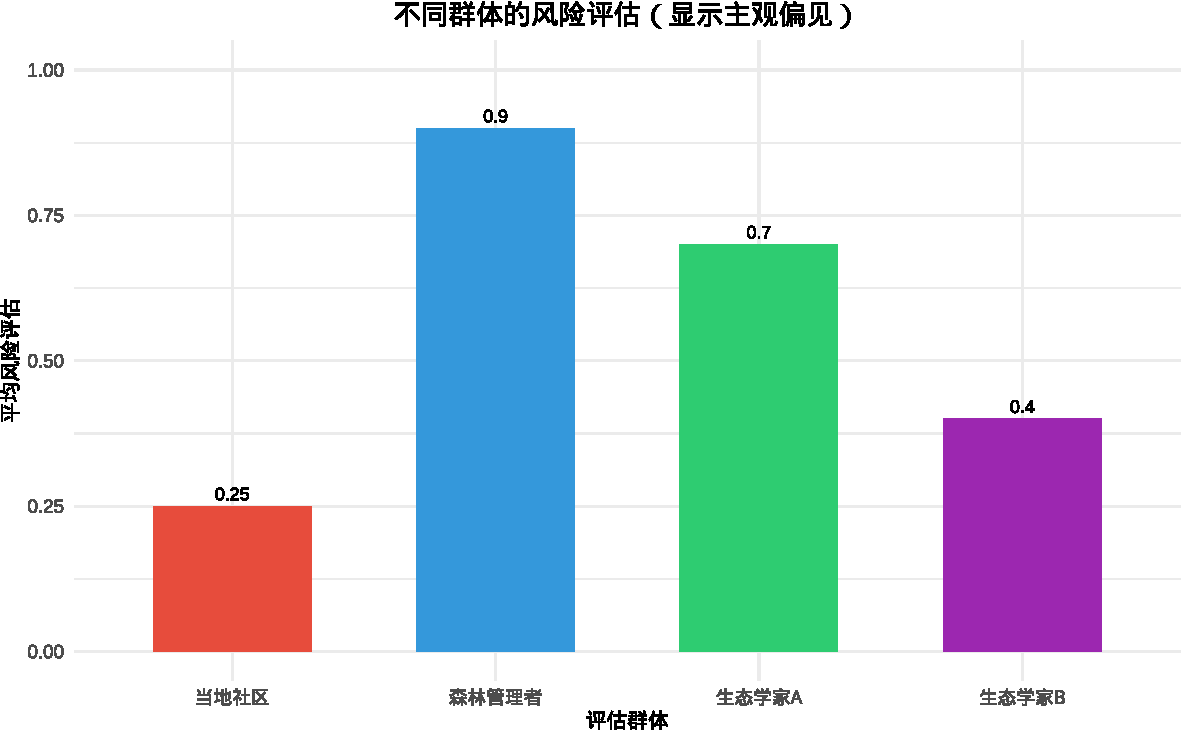
\includegraphics{02-probability_and_distribution_files/figure-latex/unnamed-chunk-14-1.pdf}

\hypertarget{ux7d2fux79efux6982ux7387ux5206ux5e03ux4eceux53efux80fdux6027ux5230ux786eux5b9aux6027}{%
\subsection{累积概率分布:从可能性到确定性}\label{ux7d2fux79efux6982ux7387ux5206ux5e03ux4eceux53efux80fdux6027ux5230ux786eux5b9aux6027}}

除了了解每种植物被选择的概率,我们有时还需要回答这样的问题:``蚱蜢选择黑麦草或混合草甸的概率是多少?''或者''选择价值较低的植物(三叶草)的概率是多少?``这些问题引导我们认识\textbf{累积概率分布}。

累积概率分布描述的是随机变量取值小于或等于某个特定值的概率。对于我们的蚱蜢午餐选择问题,我们可以构建如下的累积分布:

\begin{longtable}[]{@{}lll@{}}
\toprule\noalign{}
随机变量 X 的取值 & 概率 P(X) & 累积概率 F(x) = P(X ≤ x) \\
\midrule\noalign{}
\endhead
\bottomrule\noalign{}
\endlastfoot
1 (黑麦草) & 0.64 & 0.64 \\
2 (混合草甸) & 0.29 & 0.93 \\
3 (三叶草) & 0.07 & 1.00 \\
\end{longtable}

这里的累积概率告诉我们:
- 蚱蜢选择黑麦草的概率是 0.64
- 蚱蜢选择黑麦草\textbf{或}混合草甸的概率是 0.64 + 0.29 = 0.93
- 蚱蜢选择任意一种植物的概率是 1.00(必然事件)

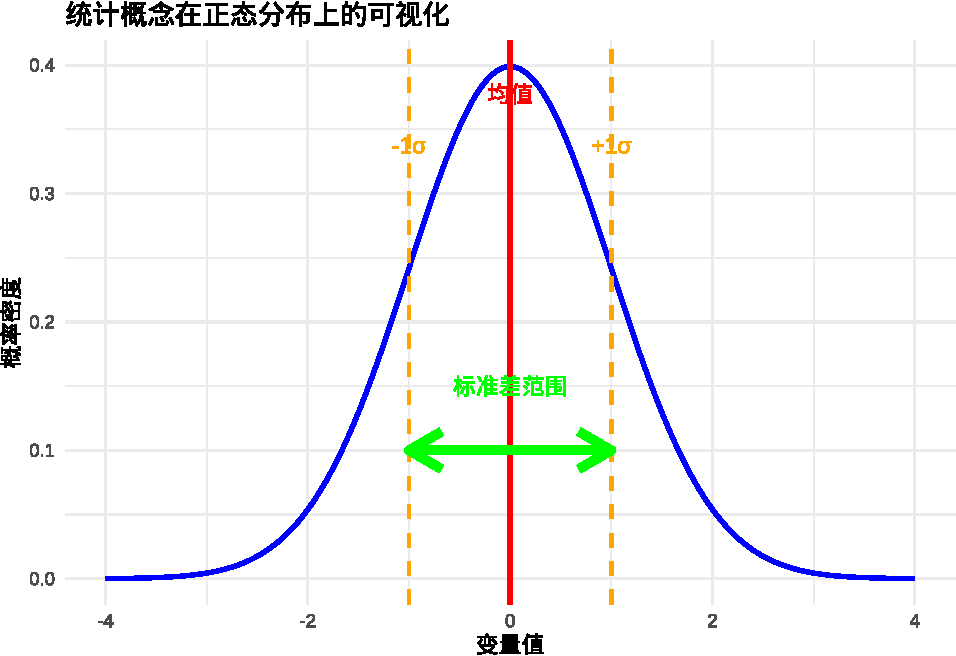
\includegraphics{02-probability_and_distribution_files/figure-latex/unnamed-chunk-15-1.pdf}

累积概率分布图呈现为阶梯函数,在每个可能的取值处跳跃,跳跃的高度等于该取值的概率。这种分布特别有用,因为它:

\begin{enumerate}
\def\labelenumi{\arabic{enumi}.}
\tightlist
\item
  \textbf{回答区间概率问题}:我们可以直接读出 P(X ≤ 2) = 0.93\\
\item
  \textbf{计算任意事件的概率}:P(X \textgreater{} 2) = 1 - P(X ≤ 2) = 1 - 0.93 = 0.07\\
\item
  \textbf{提供决策支持}:如果我们想知道''蚱蜢选择营养价值较高的植物(黑麦草或混合草甸)的概率'',累积分布直接给出了答案:0.93
\end{enumerate}

在生态学中,累积概率分布广泛应用于风险评估、资源分配决策和种群管理策略制定。

\begin{Shaded}
\begin{Highlighting}[]
\CommentTok{\# R语言中的概率分布函数家族}
\FunctionTok{cat}\NormalTok{(}\StringTok{"R为各种概率分布提供了完整的函数家族,每个分布都包含四类核心函数:}\SpecialCharTok{\textbackslash{}n}\StringTok{"}\NormalTok{)}
\end{Highlighting}
\end{Shaded}

\begin{verbatim}
## R为各种概率分布提供了完整的函数家族,每个分布都包含四类核心函数:
\end{verbatim}

\begin{Shaded}
\begin{Highlighting}[]
\FunctionTok{cat}\NormalTok{(}\StringTok{"{-} d*: 概率密度/质量函数 (density)}\SpecialCharTok{\textbackslash{}n}\StringTok{"}\NormalTok{)}
\end{Highlighting}
\end{Shaded}

\begin{verbatim}
## - d*: 概率密度/质量函数 (density)
\end{verbatim}

\begin{Shaded}
\begin{Highlighting}[]
\FunctionTok{cat}\NormalTok{(}\StringTok{"{-} p*: 累积分布函数 (probability)}\SpecialCharTok{\textbackslash{}n}\StringTok{"}\NormalTok{)}
\end{Highlighting}
\end{Shaded}

\begin{verbatim}
## - p*: 累积分布函数 (probability)
\end{verbatim}

\begin{Shaded}
\begin{Highlighting}[]
\FunctionTok{cat}\NormalTok{(}\StringTok{"{-} q*: 分位数函数 (quantile)}\SpecialCharTok{\textbackslash{}n}\StringTok{"}\NormalTok{)}
\end{Highlighting}
\end{Shaded}

\begin{verbatim}
## - q*: 分位数函数 (quantile)
\end{verbatim}

\begin{Shaded}
\begin{Highlighting}[]
\FunctionTok{cat}\NormalTok{(}\StringTok{"{-} r*: 随机数生成函数 (random)}\SpecialCharTok{\textbackslash{}n\textbackslash{}n}\StringTok{"}\NormalTok{)}
\end{Highlighting}
\end{Shaded}

\begin{verbatim}
## - r*: 随机数生成函数 (random)
\end{verbatim}

\begin{Shaded}
\begin{Highlighting}[]
\FunctionTok{cat}\NormalTok{(}\StringTok{"例如,对于正态分布:}\SpecialCharTok{\textbackslash{}n}\StringTok{"}\NormalTok{)}
\end{Highlighting}
\end{Shaded}

\begin{verbatim}
## 例如,对于正态分布:
\end{verbatim}

\begin{Shaded}
\begin{Highlighting}[]
\FunctionTok{cat}\NormalTok{(}\StringTok{"dnorm(x, mean, sd)    \# 概率密度函数}\SpecialCharTok{\textbackslash{}n}\StringTok{"}\NormalTok{)}
\end{Highlighting}
\end{Shaded}

\begin{verbatim}
## dnorm(x, mean, sd)    # 概率密度函数
\end{verbatim}

\begin{Shaded}
\begin{Highlighting}[]
\FunctionTok{cat}\NormalTok{(}\StringTok{"pnorm(q, mean, sd)    \# 累积分布函数}\SpecialCharTok{\textbackslash{}n}\StringTok{"}\NormalTok{)}
\end{Highlighting}
\end{Shaded}

\begin{verbatim}
## pnorm(q, mean, sd)    # 累积分布函数
\end{verbatim}

\begin{Shaded}
\begin{Highlighting}[]
\FunctionTok{cat}\NormalTok{(}\StringTok{"qnorm(p, mean, sd)    \# 分位数函数}\SpecialCharTok{\textbackslash{}n}\StringTok{"}\NormalTok{)}
\end{Highlighting}
\end{Shaded}

\begin{verbatim}
## qnorm(p, mean, sd)    # 分位数函数
\end{verbatim}

\begin{Shaded}
\begin{Highlighting}[]
\FunctionTok{cat}\NormalTok{(}\StringTok{"rnorm(n, mean, sd)    \# 随机数生成}\SpecialCharTok{\textbackslash{}n\textbackslash{}n}\StringTok{"}\NormalTok{)}
\end{Highlighting}
\end{Shaded}

\begin{verbatim}
## rnorm(n, mean, sd)    # 随机数生成
\end{verbatim}

\begin{Shaded}
\begin{Highlighting}[]
\FunctionTok{cat}\NormalTok{(}\StringTok{"这种统一的命名约定使得在R中学习和使用各种分布变得非常直观}\SpecialCharTok{\textbackslash{}n}\StringTok{"}\NormalTok{)}
\end{Highlighting}
\end{Shaded}

\begin{verbatim}
## 这种统一的命名约定使得在R中学习和使用各种分布变得非常直观
\end{verbatim}

R语言为概率分布提供了强大的支持,内置了数十种常见的概率分布函数。每种分布都遵循统一的命名模式,包含四个核心函数:

\begin{itemize}
\tightlist
\item
  \textbf{概率密度/质量函数} (d*): 计算特定取值的概率密度或质量
\item
  \textbf{累积分布函数} (p*): 计算小于等于某个值的累积概率
\item
  \textbf{分位数函数} (q*): 根据概率值反推对应的分位数
\item
  \textbf{随机数生成函数} (r*): 从该分布中生成随机样本
\end{itemize}

这种系统化的函数设计使得生态学家能够轻松地进行概率计算、统计推断和随机模拟。

\begin{longtable}[]{@{}
  >{\raggedright\arraybackslash}p{(\columnwidth - 6\tabcolsep) * \real{0.2500}}
  >{\raggedright\arraybackslash}p{(\columnwidth - 6\tabcolsep) * \real{0.2500}}
  >{\raggedright\arraybackslash}p{(\columnwidth - 6\tabcolsep) * \real{0.2500}}
  >{\raggedright\arraybackslash}p{(\columnwidth - 6\tabcolsep) * \real{0.2500}}@{}}
\toprule\noalign{}
\begin{minipage}[b]{\linewidth}\raggedright
分布类型
\end{minipage} & \begin{minipage}[b]{\linewidth}\raggedright
生态学应用场景
\end{minipage} & \begin{minipage}[b]{\linewidth}\raggedright
R函数前缀
\end{minipage} & \begin{minipage}[b]{\linewidth}\raggedright
主要参数
\end{minipage} \\
\midrule\noalign{}
\endhead
\bottomrule\noalign{}
\endlastfoot
二元选择分布 & 生物行为的是/否决策 & \texttt{binom} & 试验次数、成功概率 \\
计数分布 & 种群数量、事件发生次数 & \texttt{pois} & 平均发生率 \\
等待时间分布 & 生物事件间隔时间 & \texttt{geom}, \texttt{nbinom} & 成功概率、目标次数 \\
多元选择分布 & 多物种竞争、资源分配 & \texttt{multinom} & 试验次数、各类概率 \\
连续分布 & 生物体尺寸、环境变量 & \texttt{norm}, \texttt{unif} & 均值、标准差等 \\
\end{longtable}

这些分布函数为生态学研究提供了强大的数学工具,帮助我们量化自然界的随机现象。

\hypertarget{ux5348ux9910ux83dcux5355ux79bbux6563ux968fux673aux53d8ux91cfux7684ux5206ux5e03ux5bb6ux65cf}{%
\section{午餐菜单:离散随机变量的分布家族}\label{ux5348ux9910ux83dcux5355ux79bbux6563ux968fux673aux53d8ux91cfux7684ux5206ux5e03ux5bb6ux65cf}}

我们已经成功地为蚱蜢的午餐偏好创建了一个数学模型。我们定义了一个随机变量X,它就像一个聪明的代理人,将``吃哪种植物''这个文字问题,转化成了``X等于1,2,还是3?''这个数学问题。

离散型随机变量的核心特征就是:它的可能取值是有限个或可数的无限个(就像整数一样,可以一个一个数出来)。蚱蜢的选择(1,2,3)就是有限的、分立的点,而不是连续的光滑区间。我们整理出的那张概率表格,正是这个随机变量的概率分布。它如同一份``行为密码'',精确地告诉我们这只蚱蜢的习性。

不过,自然界的奥秘在于,许多看似不同的行为背后,可能隐藏着同一种``底层法则''。接下来,就让我们认识几位在生态学中无处不在的离散分布``明星''。

\hypertarget{ux4f2fux52aaux5229ux5206ux5e03ux4e00ux4e2aux662fux6216ux5426ux7684ux7ec8ux6781ux95eeux9898}{%
\subsection{伯努利分布:一个''是''或''否''的终极问题}\label{ux4f2fux52aaux5229ux5206ux5e03ux4e00ux4e2aux662fux6216ux5426ux7684ux7ec8ux6781ux95eeux9898}}

\textbf{故事开端:} 现在,我不再关心蚱蜢具体吃了三种植物中的哪一种,而是问一个更简单的问题:它这次进食是否选择了黑麦草? 结果只有两种:``是''(成功) 或 ``否''(失败)。这种简化的视角让我们能够专注于最本质的二元选择问题。

\textbf{数学定义:} 伯努利分布是描述单次伯努利试验结果的概率分布。伯努利试验具有三个基本特征:
1. 每次试验只有两种可能的结果(成功/失败)
2. 每次试验中成功的概率\(p\)保持不变
3. 各次试验相互独立

\textbf{概率函数表达式:} 伯努利分布的概率质量函数为:

\[P(X = x) = \begin{cases}
p & \text{如果 } x = 1 \\
1-p & \text{如果 } x = 0
\end{cases}\]

或者更简洁地表示为:
\[P(X = x) = p^x(1-p)^{1-x}, \quad x = 0,1\]

其中,\(X\)是伯努利随机变量,\(p\)是成功的概率(\(0 \leq p \leq 1\))。

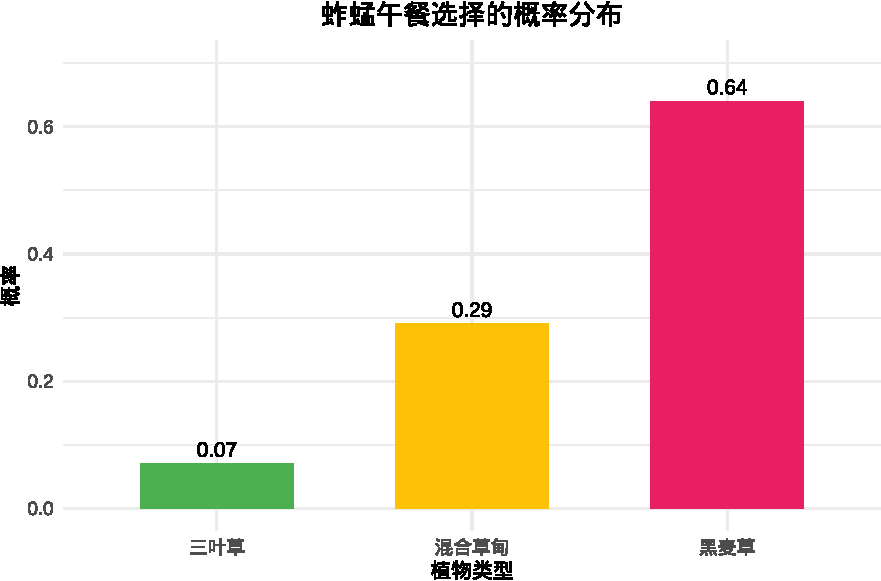
\includegraphics{02-probability_and_distribution_files/figure-latex/unnamed-chunk-17-1.pdf}

\textbf{生态学肖像:}

伯努利分布在生态学中无处不在,它描述的是那些具有二元结局的自然现象:

\begin{itemize}
\tightlist
\item
  \textbf{一颗种子是否发芽?} - 发芽(成功)或不发芽(失败)
\item
  \textbf{一只雏鸟能否成功活到离巢?} - 存活(成功)或死亡(失败)
\item
  \textbf{一次野外调查中,一个样方里是否出现了目标物种?} - 出现(成功)或不出现(失败)
\item
  \textbf{一只昆虫是否被天敌捕食?} - 被捕食(成功)或逃脱(失败)
\item
  \textbf{一片叶子是否被昆虫取食?} - 被取食(成功)或完好(失败)
\end{itemize}

\textbf{生态学意义:}

伯努利分布虽然简单,但它是构建更复杂生态学模型的基础。许多重要的生态学分布,如二项分布、几何分布、负二项分布等,都是建立在多次独立伯努利试验的基础之上。理解伯努利分布有助于我们:

\begin{enumerate}
\def\labelenumi{\arabic{enumi}.}
\tightlist
\item
  \textbf{量化二元生态过程}:将定性的生态现象转化为可量化的概率
\item
  \textbf{建立基准模型}:为更复杂的生态模型提供理论基础
\item
  \textbf{进行统计推断}:基于二元数据估计生态过程的参数
\item
  \textbf{风险评估}:评估生态事件发生的可能性
\end{enumerate}

伯努利分布的美妙之处在于它的简洁性和普适性。尽管生态系统的复杂性远超简单的二元选择,但通过将复杂问题分解为基本的伯努利试验,我们能够逐步建立起理解自然界的数学模型框架。

\hypertarget{ux4e8cux9879ux5206ux5e03ux91cdux590dux662fux975eux9898ux7684ux8ba1ux6570ux6cd5ux5219}{%
\subsection{二项分布:重复''是非题''的计数法则}\label{ux4e8cux9879ux5206ux5e03ux91cdux590dux662fux975eux9898ux7684ux8ba1ux6570ux6cd5ux5219}}

\textbf{故事延续:} 现在,我连续观察蚱蜢的10次进食选择。每一次选择,都是一个独立的伯努利试验(是否吃黑麦草)。我关心的问题是:在这10次观察中,它总共有多大概率有恰好7次选择了黑麦草?或者,至少有8次?这种从单次试验扩展到多次试验的视角,引导我们认识二项分布。

\textbf{数学定义:} 二项分布描述的是在\(n\)次独立的伯努利试验中,成功次数\(k\)的概率分布。二项试验满足以下条件:
1. 试验由\(n\)次相同的伯努利试验组成
2. 每次试验只有两种可能的结果(成功/失败)
3. 每次试验的成功概率\(p\)保持不变
4. 各次试验相互独立

\textbf{概率函数表达式:} 二项分布的概率质量函数为:

\[P(X = k) = \binom{n}{k} p^k (1-p)^{n-k}, \quad k = 0, 1, 2, \ldots, n\]

其中:
- \(X\)是二项随机变量,表示成功的次数
- \(n\)是试验总次数
- \(k\)是成功次数
- \(p\)是每次试验的成功概率
- \(\binom{n}{k} = \frac{n!}{k!(n-k)!}\)是二项系数

\textbf{分布特性:}
- 期望值:\(E[X] = np\)
- 方差:\(Var(X) = np(1-p)\)
- 当\(p=0.5\)时,分布对称;当\(p<0.5\)时右偏,\(p>0.5\)时左偏

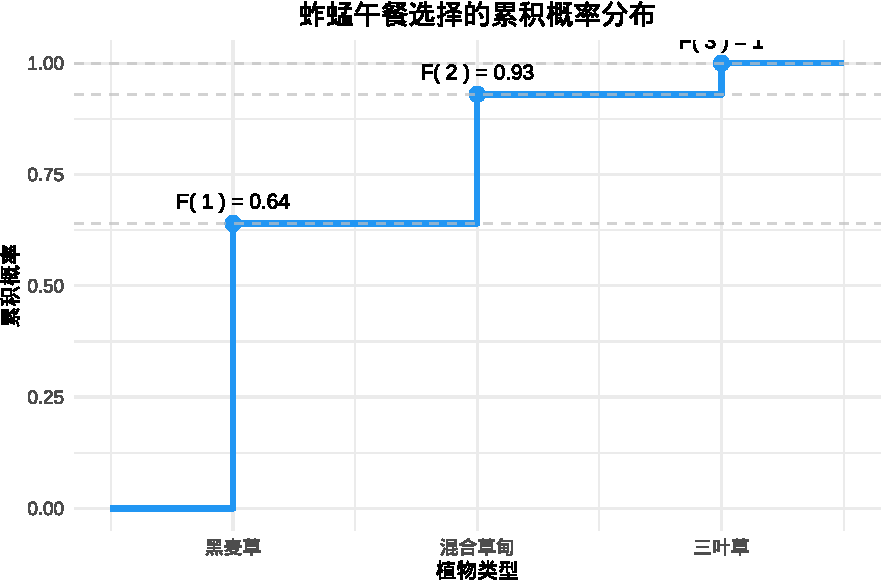
\includegraphics{02-probability_and_distribution_files/figure-latex/unnamed-chunk-18-1.pdf}

\textbf{生态学肖像:}

二项分布在生态学中广泛应用于计数型数据的建模:

\begin{itemize}
\tightlist
\item
  \textbf{播种100颗同种种子,最终成功发芽的数量\(k\)服从二项分布}(\(n=100\),\(p=\)发芽率)
\item
  \textbf{从一个大种群中随机捕获并标记50只动物,放回后再次随机捕获50只,其中被标记个体的数量\(k\)也服从二项分布}。这正是标记重捕法的理论核心!
\item
  \textbf{一片森林中,随机选择的100棵树中有病害的树木数量}
\item
  \textbf{一次生态调查中,在50个样方中发现目标物种的样方数量}
\item
  \textbf{一个鸟类种群中,在繁殖季节成功孵化的雏鸟数量}
\end{itemize}

\textbf{生态学意义:}

二项分布是伯努利分布的自然延伸,它将单个二元事件的概率模型扩展到多个独立事件的计数模型。在生态学研究中,二项分布帮助我们:

\begin{enumerate}
\def\labelenumi{\arabic{enumi}.}
\tightlist
\item
  \textbf{种群估计}:通过标记重捕法估计种群大小
\item
  \textbf{患病率研究}:估计疾病在种群中的传播程度
\item
  \textbf{物种分布}:量化物种在特定区域的分布概率
\item
  \textbf{繁殖成功率}:评估物种的繁殖表现
\item
  \textbf{抽样设计}:优化生态调查的样本大小设计
\end{enumerate}

二项分布的美妙之处在于它将复杂的生态计数问题简化为基本的概率计算,为我们提供了量化生态现象的有力工具。

\hypertarget{ux591aux9879ux5f0fux5206ux5e03ux591aux5143ux9009ux62e9ux7684ux5168ux666fux56fe}{%
\subsection{多项式分布:多元选择的''全景图''}\label{ux591aux9879ux5f0fux5206ux5e03ux591aux5143ux9009ux62e9ux7684ux5168ux666fux56fe}}

\textbf{故事视角扩展:} 二项分布处理的是''是/否''的二元选择,但生态学中我们常常面临更复杂的多元选择。回到蚱蜢的午餐选择,现在我想知道:在10次进食观察中,它恰好有6次选择黑麦草、3次选择混合草甸、1次选择三叶草的概率是多少?这种对多个类别同时计数的需求,引导我们认识多项式分布。

\textbf{数学定义:} 多项式分布是二项分布向多个类别的自然推广,描述的是在\(n\)次独立试验中,每个类别出现特定次数的联合概率分布。多项式试验满足以下条件:
1. 每次试验有\(k\)个可能的结果(类别)
2. 每个结果发生的概率分别为\(p_1, p_2, \ldots, p_k\),且\(\sum_{i=1}^k p_i = 1\)
3. 各次试验相互独立
4. 试验结果互斥且完备

\textbf{概率函数表达式:} 多项式分布的概率质量函数为:

\[P(X_1 = x_1, X_2 = x_2, \ldots, X_k = x_k) = \frac{n!}{x_1! x_2! \cdots x_k!} p_1^{x_1} p_2^{x_2} \cdots p_k^{x_k}\]

其中:
- \(X_i\)表示第\(i\)个类别出现的次数
- \(x_i\)是第\(i\)个类别的实际观察次数,且\(\sum_{i=1}^k x_i = n\)
- \(n\)是总的试验次数
- \(p_i\)是第\(i\)个类别发生的概率
- \(\frac{n!}{x_1! x_2! \cdots x_k!}\)是多项式系数

\textbf{分布特性:}
- 每个类别的边际分布都是二项分布:\(X_i \sim \text{Binomial}(n, p_i)\)
- 期望值:\(E[X_i] = np_i\)
- 方差:\(Var(X_i) = np_i(1-p_i)\)
- 协方差:\(Cov(X_i, X_j) = -np_i p_j\)(\(i \neq j\))
- 当\(k=2\)时,多项式分布退化为二项分布

\begin{verbatim}
## 
## Attaching package: 'dplyr'
\end{verbatim}

\begin{verbatim}
## The following objects are masked from 'package:stats':
## 
##     filter, lag
\end{verbatim}

\begin{verbatim}
## The following objects are masked from 'package:base':
## 
##     intersect, setdiff, setequal, union
\end{verbatim}

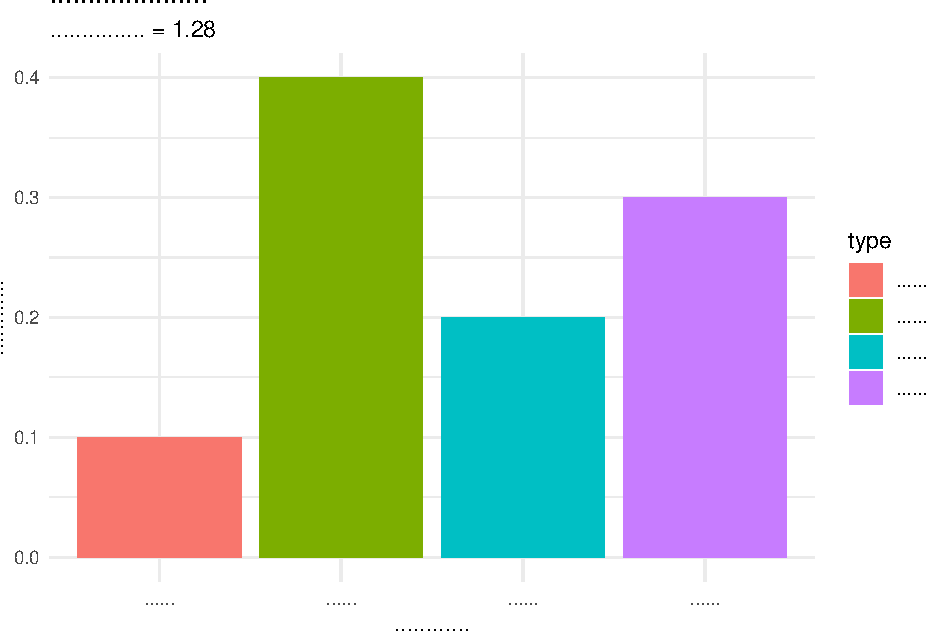
\includegraphics{02-probability_and_distribution_files/figure-latex/unnamed-chunk-19-1.pdf}

\textbf{生态学肖像:}

多项式分布在生态学中广泛应用于多类别计数数据的建模:

\begin{itemize}
\tightlist
\item
  \textbf{一片森林中,不同树种幼苗数量的联合分布} - 描述植物群落的组成结构
\item
  \textbf{一次鸟类调查中,不同物种出现次数的联合概率} - 分析鸟类群落的多样性模式
\item
  \textbf{一个湖泊中,不同浮游生物类群数量的分布} - 研究水生生态系统的营养结构
\item
  \textbf{一次昆虫采集样本中,不同科属昆虫数量的分布} - 量化昆虫群落的分类组成
\item
  \textbf{一个动物种群的年龄结构分布} - 分析种群动态的多类别特征
\end{itemize}

\textbf{生态学意义:}

多项式分布是生态学中描述多变量计数数据的核心工具,它帮助我们:

\begin{enumerate}
\def\labelenumi{\arabic{enumi}.}
\tightlist
\item
  \textbf{群落生态学}:量化物种组成的联合概率分布
\item
  \textbf{多样性研究}:分析多物种共存模式的概率特征
\item
  \textbf{资源分配}:研究生物对不同资源的选择偏好
\item
  \textbf{种群结构}:描述年龄、性别等多类别特征的分布
\item
  \textbf{生态监测}:设计多变量生态调查的统计框架
\end{enumerate}

多项式分布的美妙之处在于它能够同时捕捉多个生态类别的联合分布模式,为我们理解生态系统的复杂性和多样性提供了全面的数学框架。

\hypertarget{ux6ccaux677eux5206ux5e03ux7f55ux89c1ux4e8bux4ef6ux7684ux4f4eux8bedux8005}{%
\subsection{泊松分布:罕见事件的''低语者''}\label{ux6ccaux677eux5206ux5e03ux7f55ux89c1ux4e8bux4ef6ux7684ux4f4eux8bedux8005}}

\textbf{故事新篇:} 这次,我不固定观察次数,而是固定观察时间。我坐在草地上,用一个小时的时间,记录下这只蚱蜢做出剧烈警戒性跳跃的次数。这种跳跃并不频繁,可能一次,可能两次,也可能一次都没有。在一个很短的时间间隔内,发生一次跳跃的概率很小,且事件彼此独立。这种对稀有事件计数的需求,引导我们认识泊松分布。

\textbf{数学定义:} 泊松分布描述的是在固定时间间隔、固定面积或固定体积内,稀有事件发生次数的概率分布。泊松过程满足以下条件:
1. 事件在任意小的时间间隔内发生的概率与时间间隔长度成正比
2. 在不相交的时间间隔内,事件发生次数相互独立
3. 事件在任意时间点发生的概率相同(平稳性)
4. 在极短时间间隔内,发生两次或以上事件的概率可以忽略

\textbf{概率函数表达式:} 泊松分布的概率质量函数为:

\[P(X = k) = \frac{\lambda^k e^{-\lambda}}{k!}, \quad k = 0, 1, 2, \ldots\]

其中:
- \(X\)是泊松随机变量,表示事件发生的次数
- \(\lambda\)是单位时间(或单位面积/体积)内事件发生的平均次数
- \(k\)是实际观察到的事件次数
- \(e\)是自然对数的底(约等于2.71828)

\textbf{分布特性:}
- 期望值:\(E[X] = \lambda\)
- 方差:\(Var(X) = \lambda\)(期望等于方差是泊松分布的重要特征)
- 当\(\lambda\)较小时,分布右偏;当\(\lambda\)增大时,分布逐渐接近正态分布
- 泊松分布是二项分布在\(n \to \infty\),\(p \to 0\),且\(np = \lambda\)时的极限情况

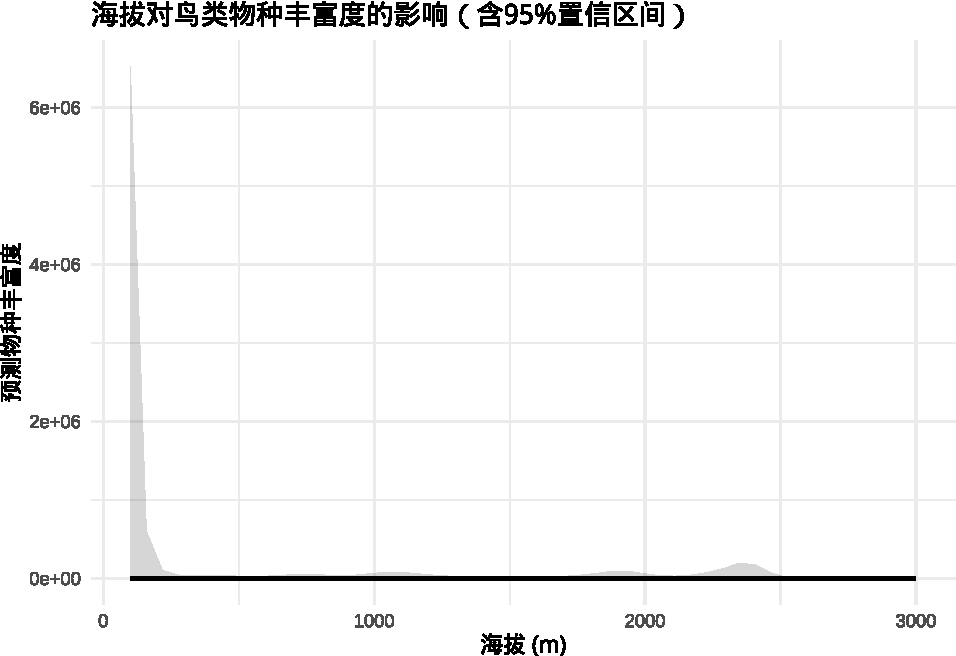
\includegraphics{02-probability_and_distribution_files/figure-latex/unnamed-chunk-20-1.pdf}

\textbf{生态学肖像:}

泊松分布在生态学中广泛应用于稀有事件和空间分布的研究:

\begin{itemize}
\tightlist
\item
  \textbf{一平方米的森林样地中,某种珍稀兰花的株数} - 描述稀有物种的空间分布
\item
  \textbf{一台红外相机在一天内,拍摄到某种神秘夜行兽的次数} - 监测稀有动物的活动频率
\item
  \textbf{一毫升海水中的浮游生物数量} - 量化微生物的密度分布
\item
  \textbf{一片草原上,单位面积内某种昆虫的巢穴数量} - 研究昆虫的空间分布模式
\item
  \textbf{一个湖泊中,特定时间段内鱼类跃出水面的次数} - 记录稀有行为的发生频率
\end{itemize}

\textbf{生态学意义:}

泊松分布是生态学中描述随机分布模式的重要工具,它帮助我们:

\begin{enumerate}
\def\labelenumi{\arabic{enumi}.}
\tightlist
\item
  \textbf{物种分布研究}:判断物种在空间上是否随机分布
\item
  \textbf{种群密度估计}:通过单位面积内的个体数估计总体密度
\item
  \textbf{行为生态学}:量化稀有行为的发生频率
\item
  \textbf{保护生物学}:评估稀有物种的分布状况
\item
  \textbf{生态监测}:设计合理的监测方案和样本大小
\end{enumerate}

泊松分布的美妙之处在于它用一个简单的参数\(\lambda\)就描述了复杂生态现象的概率规律,为我们理解自然界的随机性提供了简洁而强大的数学工具。

\hypertarget{ux51e0ux4f55ux5206ux5e03ux7b49ux5f85ux7b2cux4e00ux6b21ux6210ux529fux7684ux8010ux5fc3}{%
\subsection{几何分布:等待''第一次成功''的耐心}\label{ux51e0ux4f55ux5206ux5e03ux7b49ux5f85ux7b2cux4e00ux6b21ux6210ux529fux7684ux8010ux5fc3}}

\textbf{故事视角转换:} 想象现在是清晨,蚱蜢开始了它的第一次觅食。我好奇的是:它需要尝试多少次,才能第一次成功吃到它最爱的黑麦草? 也许第一次就成功了(X=1),也许前两次都去了别处,第三次才成功(X=3)。这种对''第一次成功''等待时间的关注,引导我们认识几何分布。

\textbf{数学定义:} 几何分布描述的是在一系列独立的伯努利试验中,首次获得成功所需要的试验次数。几何分布满足以下条件:
1. 试验由一系列相同的伯努利试验组成
2. 每次试验只有两种可能的结果(成功/失败)
3. 每次试验的成功概率\(p\)保持不变
4. 各次试验相互独立
5. 试验持续进行直到第一次成功出现

\textbf{概率函数表达式:} 几何分布的概率质量函数为:

\[P(X = k) = (1-p)^{k-1} p, \quad k = 1, 2, 3, \ldots\]

其中:
- \(X\)是几何随机变量,表示首次成功所需的试验次数
- \(k\)是试验次数(\(k \geq 1\))
- \(p\)是每次试验的成功概率
- \((1-p)^{k-1}\)表示前\(k-1\)次都失败的概率

\textbf{分布特性:}
- 期望值:\(E[X] = \frac{1}{p}\)
- 方差:\(Var(X) = \frac{1-p}{p^2}\)
- 无记忆性:\(P(X > m+n \mid X > m) = P(X > n)\),即过去的失败不影响未来的成功概率
- 当\(p\)较小时,分布右偏严重;当\(p\)接近1时,分布集中在较小的\(k\)值

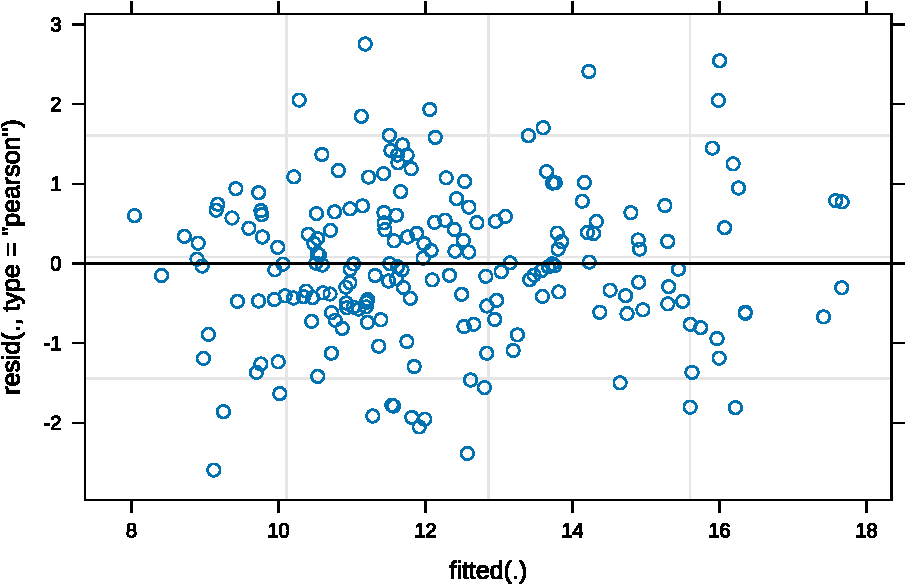
\includegraphics{02-probability_and_distribution_files/figure-latex/unnamed-chunk-21-1.pdf}

\textbf{生态学肖像:}

几何分布在生态学中广泛应用于''等待时间''和''首次成功''的研究:

\begin{itemize}
\tightlist
\item
  \textbf{一只捕食者需要巡视几个洞穴,才能发现第一个有猎物的} - 描述捕食效率
\item
  \textbf{一只传粉昆虫需要访问多少朵花,才能第一次成功获得花蜜} - 研究传粉行为效率
\item
  \textbf{一颗种子需要经历多少个雨季,才能第一次成功发芽} - 分析种子萌发模式
\item
  \textbf{一只候鸟需要尝试多少次,才能第一次成功找到迁徙路线} - 研究学习行为
\item
  \textbf{一个植物种群需要经过多少代,才能第一次出现抗病突变} - 分析进化过程
\end{itemize}

\textbf{生态学意义:}

几何分布是生态学中描述''等待过程''的重要工具,它帮助我们:

\begin{enumerate}
\def\labelenumi{\arabic{enumi}.}
\tightlist
\item
  \textbf{行为生态学}:量化动物行为的效率和成功率
\item
  \textbf{种群动态}:分析种群恢复和重建的时间过程
\item
  \textbf{进化生态学}:研究适应性特征的进化时间尺度
\item
  \textbf{保护生物学}:评估濒危物种恢复的可能性
\item
  \textbf{生态恢复}:预测生态系统恢复所需的时间
\end{enumerate}

几何分布的美妙之处在于它用一个简单的参数\(p\)就描述了复杂生态过程中的等待时间规律,特别是其''无记忆性''特征,使得我们可以专注于当前的生态过程而不受历史影响。

\hypertarget{ux8d1fux4e8cux9879ux5206ux5e03ux7b49ux5f85ux6700ux540eux4e00ux6b21ux6210ux529fux7684ux8010ux5fc3}{%
\subsection{负二项分布:等待''最后一次成功''的耐心}\label{ux8d1fux4e8cux9879ux5206ux5e03ux7b49ux5f85ux6700ux540eux4e00ux6b21ux6210ux529fux7684ux8010ux5fc3}}

\textbf{故事视角深化:} 几何分布关注的是''第一次成功'',但生态学中我们常常需要更复杂的等待模式。比如,我想知道:这只蚱蜢需要尝试多少次,才能\textbf{第三次}成功吃到黑麦草?这种对''第r次成功''等待时间的关注,引导我们认识负二项分布。

\textbf{数学定义:} 负二项分布描述的是在一系列独立的伯努利试验中,获得第r次成功所需要的试验次数。负二项分布满足以下条件:
1. 试验由一系列相同的伯努利试验组成
2. 每次试验只有两种可能的结果(成功/失败)
3. 每次试验的成功概率\(p\)保持不变
4. 各次试验相互独立
5. 试验持续进行直到第r次成功出现

\textbf{概率函数表达式:} 负二项分布的概率质量函数为:

\[P(X = k) = \binom{k-1}{r-1} p^r (1-p)^{k-r}, \quad k = r, r+1, r+2, \ldots\]

其中:
- \(X\)是负二项随机变量,表示第r次成功所需的试验次数
- \(k\)是总的试验次数(\(k \geq r\))
- \(r\)是期望的成功次数
- \(p\)是每次试验的成功概率
- \(\binom{k-1}{r-1}\)是组合数,表示前\(k-1\)次试验中安排\(r-1\)次成功的方式数

\textbf{分布特性:}
- 期望值:\(E[X] = \frac{r}{p}\)
- 方差:\(Var(X) = \frac{r(1-p)}{p^2}\)
- 当\(r=1\)时,负二项分布退化为几何分布
- 分布形状取决于\(r\)和\(p\)的值,可以呈现不同的偏斜形态

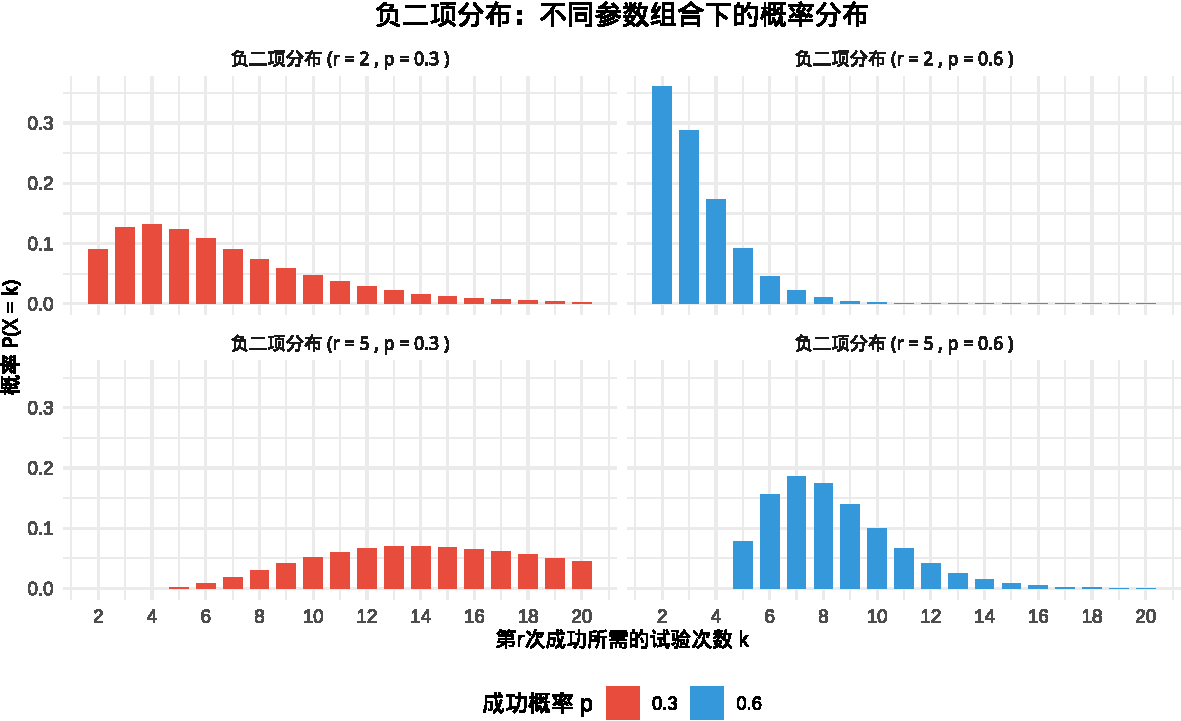
\includegraphics{02-probability_and_distribution_files/figure-latex/unnamed-chunk-22-1.pdf}

\textbf{生态学肖像:}

负二项分布在生态学中广泛应用于需要多次成功才能达到目标的场景:

\begin{itemize}
\tightlist
\item
  \textbf{一只捕食者需要捕获多少只猎物,才能满足其能量需求(第r次成功捕食)} - 描述捕食效率的累积效应
\item
  \textbf{一个植物种群需要经过多少代,才能积累到足够的有利突变(第r次有利突变)} - 分析进化过程的累积性
\item
  \textbf{一次生态调查需要设置多少个样方,才能第r次发现目标稀有物种} - 优化稀有物种监测方案
\item
  \textbf{一个生态系统需要经历多少次干扰,才会达到第r次显著的结构变化} - 研究生态系统的累积响应
\item
  \textbf{一个保护项目需要实施多少项措施,才能第r次观察到种群恢复迹象} - 评估保护措施的有效性
\end{itemize}

\textbf{生态学意义:}

负二项分布是几何分布的自然推广,它将单次成功的等待时间模型扩展到多次成功的累积等待时间模型。在生态学研究中,负二项分布帮助我们:

\begin{enumerate}
\def\labelenumi{\arabic{enumi}.}
\tightlist
\item
  \textbf{资源管理}:预测达到特定资源积累目标所需的时间或努力
\item
  \textbf{种群监测}:设计合理的监测方案来发现稀有物种
\item
  \textbf{保护规划}:评估保护措施实施的时间框架和效果
\item
  \textbf{进化研究}:分析适应性特征积累的时间尺度
\item
  \textbf{风险评估}:评估生态系统达到临界状态所需的干扰次数
\end{enumerate}

负二项分布的美妙之处在于它能够描述生态系统中''累积成功''的复杂模式,为我们理解生态过程的渐进性和累积性提供了有力的数学工具。

\hypertarget{ux5348ux9910ux6cd5ux5219ux8fdeux7eedux968fux673aux53d8ux91cfux7684ux5206ux5e03ux5bb6ux65cf}{%
\section{午餐法则:连续随机变量的分布家族}\label{ux5348ux9910ux6cd5ux5219ux8fdeux7eedux968fux673aux53d8ux91cfux7684ux5206ux5e03ux5bb6ux65cf}}

\textbf{从跳跃到体长:描绘连续世界的概率地图}

我们已经为蚱蜢的''午餐选择''绘制了一张清晰的概率分布图,那是由一根根独立的柱子组成的,因为它的选择是分门别类的(植物A、B、C)。这类变量被称为离散型随机变量,它们的取值是可数的。

但现在,让我们拿起尺子和高速摄像机,关注一些更细微、更流畅的特征。比如,这只蚱蜢的体长是多少厘米?或者它受到惊吓时,一次跳跃的距离是多少米?这些数值,可以是3.15厘米,也可以是3.151厘米,甚至在理论上可以是3.1515926\ldots 厘米。它们的取值充满了无限的可能性,充满了''连续性''。

连续型随机变量的核心特征就是:它的可能取值构成一个连续的区间,无法一一列举。在生态学中,绝大多数测量值都是连续的------温度、湿度、海拔、生物量、生长速率等等。这些变量构成了我们对自然界的量化认知基础。

\textbf{从柱子到光滑的曲线:概率密度函数}

当我们面对这样一个连续型随机变量时,之前那种''给每个特定值分配一个概率''的方法就失效了。因为任何一个精确值的概率(比如P(体长=3.15厘米))在无限的可能性面前,都几乎等于零!这就像问''在一根无限长的线上,恰好选中某个点的概率是多少?``------答案是零。

那么,我们该如何描述它的概率分布呢?聪明的做法是,我们不再关心''点''的概率,而是关心''区间''的概率。我们问的是:``这只蚱蜢的体长在3.1厘米到3.2厘米之间的概率是多少?'' 这时,概率就不再是柱子的高度,而是曲线下某一块区域的面积。

这条至关重要的曲线,就叫做\textbf{概率密度函数} 曲线。曲线本身在任意一点的高度(概率密度)并不直接代表概率,但它决定了概率的大小:曲线越高、越''胖''的区域,对应的区间概率就越大。曲线下的总面积,被定义为1,代表了所有可能性的总和(100\%)。

\textbf{数学定义:} 对于连续随机变量X,其概率密度函数\(f(x)\)满足:

\begin{enumerate}
\def\labelenumi{\arabic{enumi}.}
\tightlist
\item
  非负性:\(f(x) \geq 0\) 对所有\(x\)
\item
  规范性:\(\int_{-\infty}^{\infty} f(x) dx = 1\)
\item
  区间概率:\(P(a \leq X \leq b) = \int_a^b f(x) dx\)
\end{enumerate}

\textbf{累积分布函数:连续世界的''阶梯''}

与离散随机变量类似,连续随机变量也有其累积分布函数,定义为:

\[F(x) = P(X \leq x) = \int_{-\infty}^x f(t) dt\]

累积分布函数\(F(x)\)给出了随机变量取值小于或等于\(x\)的概率。它具有以下重要性质:

\begin{enumerate}
\def\labelenumi{\arabic{enumi}.}
\tightlist
\item
  单调不减:如果\(x_1 < x_2\),则\(F(x_1) \leq F(x_2)\)
\item
  边界条件:\(\lim_{x \to -\infty} F(x) = 0\),\(\lim_{x \to \infty} F(x) = 1\)
\item
  右连续性:\(F(x)\)在任意点\(x\)处右连续
\end{enumerate}

通过累积分布函数,我们可以方便地计算各种概率:
- \(P(a < X \leq b) = F(b) - F(a)\)
- \(P(X > x) = 1 - F(x)\)

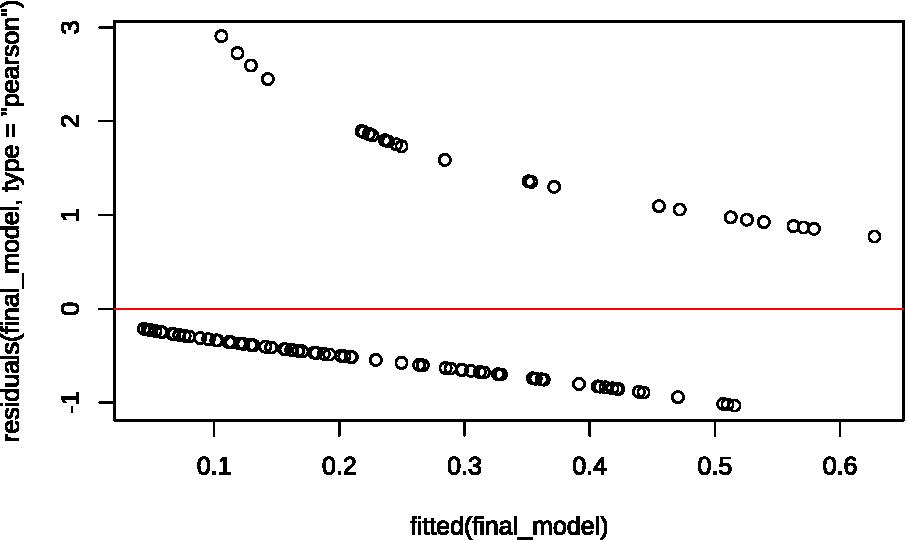
\includegraphics{02-probability_and_distribution_files/figure-latex/unnamed-chunk-23-1.pdf} 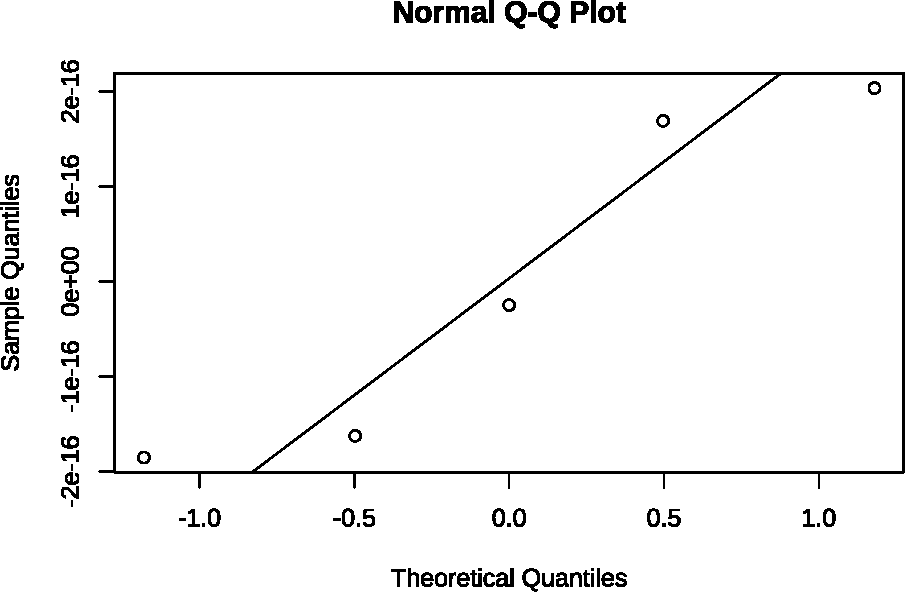
\includegraphics{02-probability_and_distribution_files/figure-latex/unnamed-chunk-23-2.pdf}

在连续变量的世界里,有几个声名显赫的''家族'',它们以特定的形态描绘了不同自然现象背后的概率规律。每个分布都有其独特的数学特性和生态学意义,共同构成了我们理解连续生态变量的工具箱。

\hypertarget{ux5747ux5300ux5206ux5e03ux7eafux7cb9ux7684ux5e73ux7b49}{%
\subsection{均匀分布:纯粹的平等}\label{ux5747ux5300ux5206ux5e03ux7eafux7cb9ux7684ux5e73ux7b49}}

\textbf{故事引入:} 想象这只蚱蜢找到了一片巨大且质地均匀的叶子,它准备开始享用午餐。这片叶子从叶尖到叶柄的长度是10厘米。蚱蜢会随机选择一个位置开始进食。它第一口吃的位置到叶尖的距离是多少厘米?可能是2厘米,也可能是5厘米,或者8厘米,每个距离被选中的可能性完全相同。这种''完全随机''的选择过程,就是均匀分布的典型场景。

\textbf{数学定义:} 均匀分布描述的是在区间\([a, b]\)内,所有取值等可能出现的概率分布。其概率密度函数为:

\[f(x) = \begin{cases}
\frac{1}{b-a} & \text{如果 } a \leq x \leq b \\
0 & \text{其他}
\end{cases}\]

\textbf{分布特性:}
- 期望值:\(E[X] = \frac{a+b}{2}\)
- 方差:\(Var(X) = \frac{(b-a)^2}{12}\)
- 在区间\([a, b]\)内,概率密度恒定

\textbf{生态学肖像:}
- \textbf{觅食行为研究}:蚱蜢在均匀资源上的随机选择行为服从均匀分布
- \textbf{资源利用模式}:当食物资源分布均匀时,动物的觅食位置选择可以建模为均匀分布
- \textbf{行为生态学实验}:在控制实验中,动物的随机选择行为可以用均匀分布来描述

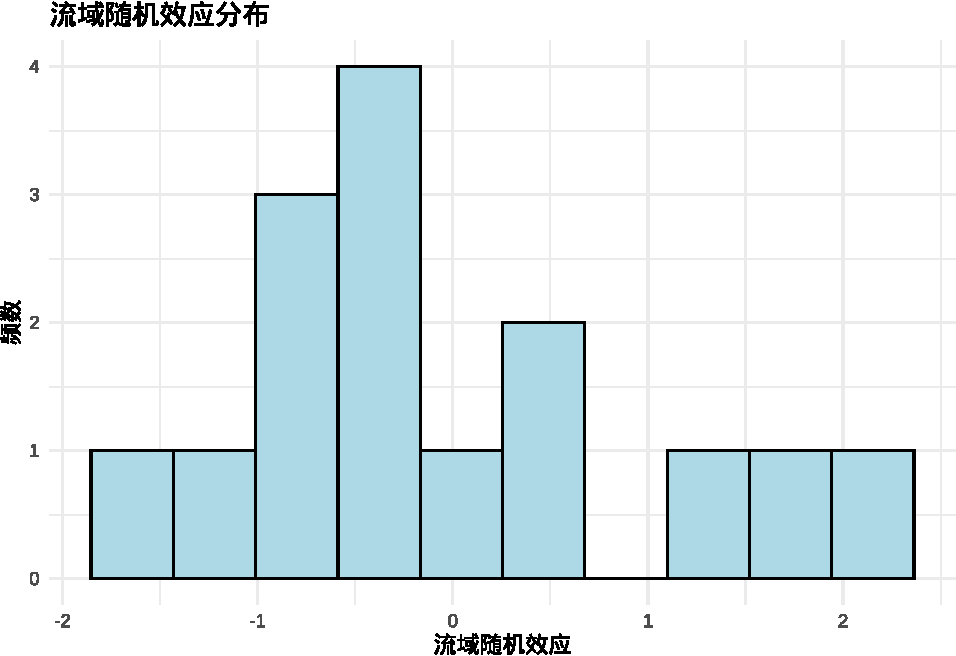
\includegraphics{02-probability_and_distribution_files/figure-latex/unnamed-chunk-24-1.pdf}

\hypertarget{ux6307ux6570ux5206ux5e03ux7b49ux5f85ux7684ux827aux672f}{%
\subsection{指数分布:等待的艺术}\label{ux6307ux6570ux5206ux5e03ux7b49ux5f85ux7684ux827aux672f}}

\textbf{故事引入:} 现在让我们关注时间维度。这只蚱蜢正在草地上专心享用午餐,但它必须时刻保持警惕。下一次被天敌(如鸟类)发现需要等待多长时间?可能是几分钟,也可能是几十分钟。这种''等待被捕食''的时间间隔,正是指数分布的用武之地。在蚱蜢的午餐过程中,这种生存威胁的随机出现模式可以用指数分布来精确描述。

\textbf{数学定义:} 指数分布描述的是泊松过程中事件发生的时间间隔。其概率密度函数为:

\[f(x) = \lambda e^{-\lambda x}, \quad x \geq 0\]

其中\(\lambda > 0\)是速率参数,表示单位时间内事件发生的平均次数。

\textbf{分布特性:}
- 期望值:\(E[X] = \frac{1}{\lambda}\)
- 方差:\(Var(X) = \frac{1}{\lambda^2}\)
- \textbf{无记忆性}:\(P(X > s + t \mid X > s) = P(X > t)\),即过去的等待不影响未来的等待时间
- 分布呈右偏,具有长尾特征

\textbf{生态学肖像:}
- \textbf{捕食风险建模}:蚱蜢在觅食过程中被捕食者发现的等待时间服从指数分布
- \textbf{生存策略研究}:无记忆性特征反映了捕食风险的随机性,帮助理解蚱蜢的警戒行为
- \textbf{行为时间模式}:动物在危险环境中的活动间隔可以用指数分布来描述
- \textbf{种群生存分析}:在高捕食压力下,个体的生存时间分布近似指数分布

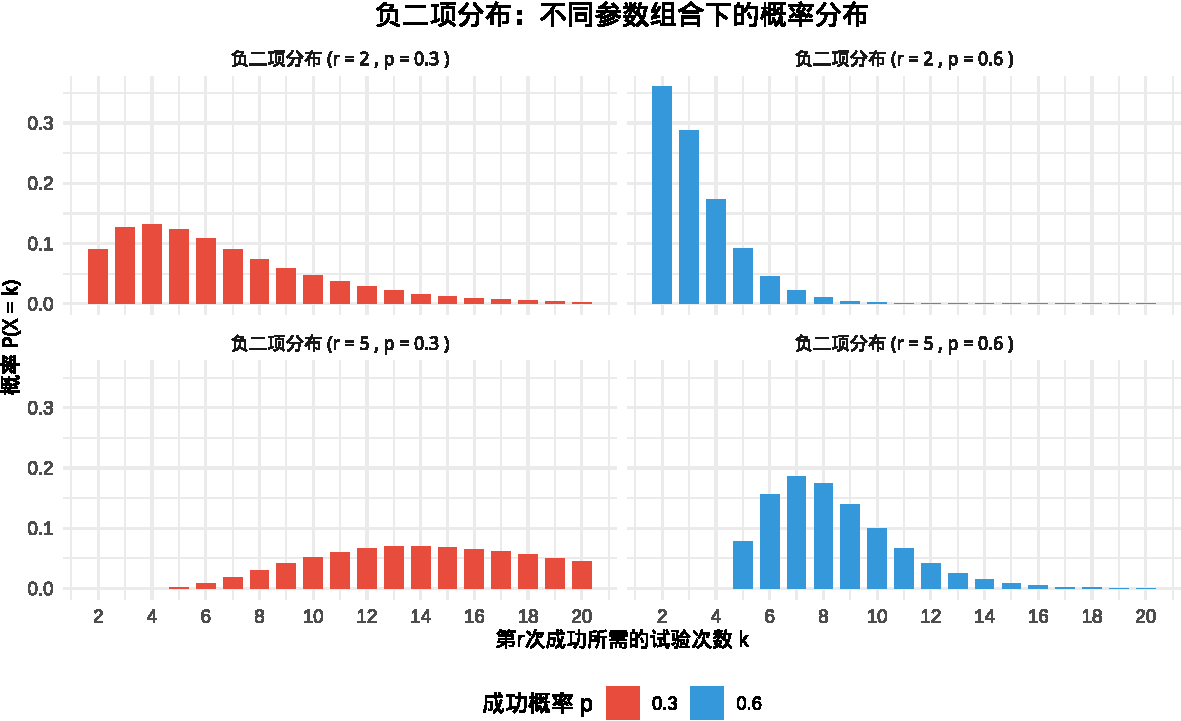
\includegraphics{02-probability_and_distribution_files/figure-latex/unnamed-chunk-25-1.pdf}

\hypertarget{ux6b63ux6001ux5206ux5e03ux9ad8ux65afux5206ux5e03ux81eaux7136ux754cux7684ux949fux5f62ux6cd5ux5219}{%
\subsection{正态分布(高斯分布):自然界的''钟形''法则}\label{ux6b63ux6001ux5206ux5e03ux9ad8ux65afux5206ux5e03ux81eaux7136ux754cux7684ux949fux5f62ux6cd5ux5219}}

\textbf{故事引入:} 仔细观察这只蚱蜢的午餐习惯,你会发现每次它吃的食物量(如叶片面积或花蜜量)存在自然的变异。大部分情况下,它吃的量都集中在某个平均值附近,极端过多或过少的摄食行为相对少见。这种''中间多,两头少''的分布模式,就是正态分布的典型特征。蚱蜢的摄食行为受到多种微小因素的共同影响,最终呈现出这种经典的钟形分布。

\textbf{数学定义:} 正态分布的概率密度函数为:

\[f(x) = \frac{1}{\sqrt{2\pi}\sigma} e^{-\frac{(x-\mu)^2}{2\sigma^2}}, \quad -\infty < x < \infty\]

其中\(\mu\)是均值(决定分布的中心位置),\(\sigma\)是标准差(决定分布的离散程度)。

\textbf{分布特性:}
- 期望值:\(E[X] = \mu\)
- 方差:\(Var(X) = \sigma^2\)
- 对称性:分布关于均值\(\mu\)对称
- 68-95-99.7法则:约68\%的数据落在\(\mu \pm \sigma\)内,95\%落在\(\mu \pm 2\sigma\)内,99.7\%落在\(\mu \pm 3\sigma\)内
- 中心极限定理:大量独立随机变量的和近似服从正态分布

\textbf{生态学肖像:}
- \textbf{摄食行为研究}:蚱蜢每次进食的食物量服从正态分布,反映其稳定的摄食模式
- \textbf{营养摄入分析}:个体间的摄食量差异可以用正态分布来描述
- \textbf{行为生态学}:动物的许多连续行为特征(如觅食时间、移动距离)近似正态分布
- \textbf{种群能量学}:通过摄食量的正态分布可以估计种群的能量摄入模式

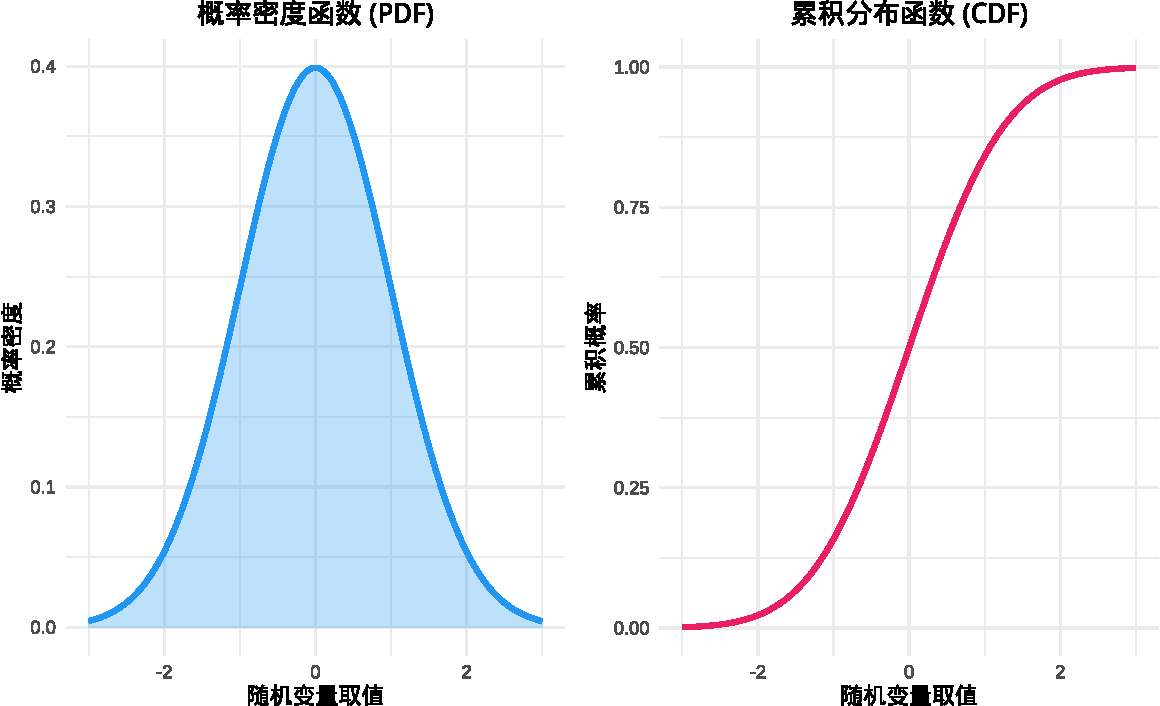
\includegraphics{02-probability_and_distribution_files/figure-latex/unnamed-chunk-26-1.pdf}

\hypertarget{ux5a01ux5e03ux5c14ux5206ux5e03ux751fux5b58ux5206ux6790ux7684ux65f6ux95f4ux6cd5ux5219}{%
\subsection{威布尔分布:生存分析的''时间法则''}\label{ux5a01ux5e03ux5c14ux5206ux5e03ux751fux5b58ux5206ux6790ux7684ux65f6ux95f4ux6cd5ux5219}}

\textbf{故事引入:} 观察这只蚱蜢的生存历程,你会发现它的死亡风险并非一成不变。在生命的早期,由于适应环境的能力较弱,死亡风险相对较高;进入成年期后,风险逐渐稳定;而到了老年期,由于生理机能衰退,死亡风险又会显著上升。这种随时间变化的死亡风险模式,正是威布尔分布能够精确描述的。蚱蜢的生存时间受到多种风险因素的综合影响,最终呈现出这种''浴盆曲线''的风险特征。

\textbf{数学定义:} 威布尔分布的概率密度函数为:

\[f(x) = \frac{k}{\lambda} \left(\frac{x}{\lambda}\right)^{k-1} e^{-(x/\lambda)^k}, \quad x \geq 0\]

其中\(k\)是形状参数(决定分布形态),\(\lambda\)是尺度参数(决定分布范围)。

\textbf{分布特性:}
- 期望值:\(E[X] = \lambda \Gamma(1 + 1/k)\)
- 方差:\(Var(X) = \lambda^2 [\Gamma(1 + 2/k) - \Gamma^2(1 + 1/k)]\)
- 生存函数:\(S(x) = e^{-(x/\lambda)^k}\)
- 风险函数:\(h(x) = \frac{k}{\lambda} \left(\frac{x}{\lambda}\right)^{k-1}\)
- 当\(k=1\)时退化为指数分布(恒定风险)
- 当\(k>1\)时风险随时间增加(老化效应)
- 当\(k<1\)时风险随时间减少(早期适应期)

\textbf{生态学肖像:}\\
- \textbf{生存分析研究}:蚱蜢的生存时间服从威布尔分布,反映其生命周期的风险变化模式\\
- \textbf{种群动态建模}:通过威布尔分布可以估计种群的死亡率模式和期望寿命\\
- \textbf{保护生物学}:濒危物种的生存时间分析有助于制定保护策略\\
- \textbf{物候学研究}:植物开花时间、动物迁徙时间等时间事件的分析

\begin{Shaded}
\begin{Highlighting}[]
\CommentTok{\# 威布尔分布:生存分析和寿命数据的分布}
\CommentTok{\# 生态学应用:动物寿命、设备故障时间、种子萌发时间等}

\CommentTok{\# 参数:形状参数k,尺度参数λ}
\NormalTok{shape\_param }\OtherTok{\textless{}{-}} \FloatTok{2.5}
\NormalTok{scale\_param }\OtherTok{\textless{}{-}} \DecValTok{10}

\CommentTok{\# 模拟蚱蜢生存时间数据}
\NormalTok{survival\_times }\OtherTok{\textless{}{-}} \FunctionTok{rweibull}\NormalTok{(}\DecValTok{200}\NormalTok{, }\AttributeTok{shape =}\NormalTok{ shape\_param, }\AttributeTok{scale =}\NormalTok{ scale\_param)}

\CommentTok{\# 描述统计}
\FunctionTok{print}\NormalTok{(}\FunctionTok{paste}\NormalTok{(}\StringTok{"样本均值:"}\NormalTok{, }\FunctionTok{round}\NormalTok{(}\FunctionTok{mean}\NormalTok{(survival\_times), }\DecValTok{2}\NormalTok{)))}
\FunctionTok{print}\NormalTok{(}\FunctionTok{paste}\NormalTok{(}\StringTok{"样本标准差:"}\NormalTok{, }\FunctionTok{round}\NormalTok{(}\FunctionTok{sd}\NormalTok{(survival\_times), }\DecValTok{2}\NormalTok{)))}

\CommentTok{\# 理论均值和方差}
\CommentTok{\# 威布尔分布的均值和方差公式}
\CommentTok{\# E[X] = λΓ(1 + 1/k)}
\CommentTok{\# Var(X) = λ²[Γ(1 + 2/k) {-} Γ²(1 + 1/k)]}
\NormalTok{theoretical\_mean }\OtherTok{\textless{}{-}}\NormalTok{ scale\_param }\SpecialCharTok{*} \FunctionTok{gamma}\NormalTok{(}\DecValTok{1} \SpecialCharTok{+} \DecValTok{1}\SpecialCharTok{/}\NormalTok{shape\_param)}
\NormalTok{theoretical\_var }\OtherTok{\textless{}{-}}\NormalTok{ scale\_param}\SpecialCharTok{\^{}}\DecValTok{2} \SpecialCharTok{*}\NormalTok{ (}\FunctionTok{gamma}\NormalTok{(}\DecValTok{1} \SpecialCharTok{+} \DecValTok{2}\SpecialCharTok{/}\NormalTok{shape\_param) }\SpecialCharTok{{-}} \FunctionTok{gamma}\NormalTok{(}\DecValTok{1} \SpecialCharTok{+} \DecValTok{1}\SpecialCharTok{/}\NormalTok{shape\_param)}\SpecialCharTok{\^{}}\DecValTok{2}\NormalTok{)}

\FunctionTok{print}\NormalTok{(}\FunctionTok{paste}\NormalTok{(}\StringTok{"理论均值:"}\NormalTok{, }\FunctionTok{round}\NormalTok{(theoretical\_mean, }\DecValTok{2}\NormalTok{)))}
\FunctionTok{print}\NormalTok{(}\FunctionTok{paste}\NormalTok{(}\StringTok{"理论方差:"}\NormalTok{, }\FunctionTok{round}\NormalTok{(theoretical\_var, }\DecValTok{2}\NormalTok{)))}

\CommentTok{\# 可视化威布尔分布}
\FunctionTok{hist}\NormalTok{(survival\_times, }\AttributeTok{breaks =} \DecValTok{30}\NormalTok{, }\AttributeTok{freq =} \ConstantTok{FALSE}\NormalTok{,}
     \AttributeTok{main =} \StringTok{"蚱蜢生存时间分布(威布尔分布)"}\NormalTok{,}
     \AttributeTok{xlab =} \StringTok{"生存时间(天)"}\NormalTok{, }\AttributeTok{ylab =} \StringTok{"密度"}\NormalTok{,}
     \AttributeTok{col =} \StringTok{"lightblue"}\NormalTok{, }\AttributeTok{xlim =} \FunctionTok{c}\NormalTok{(}\DecValTok{0}\NormalTok{, }\DecValTok{25}\NormalTok{))}

\CommentTok{\# 添加理论威布尔曲线}
\NormalTok{x\_vals }\OtherTok{\textless{}{-}} \FunctionTok{seq}\NormalTok{(}\DecValTok{0}\NormalTok{, }\DecValTok{25}\NormalTok{, }\FloatTok{0.1}\NormalTok{)}
\NormalTok{y\_vals }\OtherTok{\textless{}{-}} \FunctionTok{dweibull}\NormalTok{(x\_vals, }\AttributeTok{shape =}\NormalTok{ shape\_param, }\AttributeTok{scale =}\NormalTok{ scale\_param)}
\FunctionTok{lines}\NormalTok{(x\_vals, y\_vals, }\AttributeTok{col =} \StringTok{"red"}\NormalTok{, }\AttributeTok{lwd =} \DecValTok{2}\NormalTok{)}

\CommentTok{\# 添加生存函数曲线}
\NormalTok{survival\_vals }\OtherTok{\textless{}{-}} \DecValTok{1} \SpecialCharTok{{-}} \FunctionTok{pweibull}\NormalTok{(x\_vals, }\AttributeTok{shape =}\NormalTok{ shape\_param, }\AttributeTok{scale =}\NormalTok{ scale\_param)}
\FunctionTok{lines}\NormalTok{(x\_vals, survival\_vals, }\AttributeTok{col =} \StringTok{"blue"}\NormalTok{, }\AttributeTok{lwd =} \DecValTok{2}\NormalTok{, }\AttributeTok{lty =} \DecValTok{2}\NormalTok{)}

\FunctionTok{legend}\NormalTok{(}\StringTok{"topright"}\NormalTok{, }\AttributeTok{legend =} \FunctionTok{c}\NormalTok{(}\StringTok{"概率密度"}\NormalTok{, }\StringTok{"生存函数"}\NormalTok{),}
       \AttributeTok{col =} \FunctionTok{c}\NormalTok{(}\StringTok{"red"}\NormalTok{, }\StringTok{"blue"}\NormalTok{), }\AttributeTok{lty =} \DecValTok{1}\SpecialCharTok{:}\DecValTok{2}\NormalTok{, }\AttributeTok{lwd =} \DecValTok{2}\NormalTok{)}

\CommentTok{\# 参数估计:使用最大似然估计拟合威布尔分布}
\FunctionTok{library}\NormalTok{(fitdistrplus)}
\NormalTok{fit\_weibull }\OtherTok{\textless{}{-}} \FunctionTok{fitdist}\NormalTok{(survival\_times, }\StringTok{"weibull"}\NormalTok{)}
\FunctionTok{print}\NormalTok{(}\StringTok{"威布尔分布参数估计结果:"}\NormalTok{)}
\FunctionTok{print}\NormalTok{(}\FunctionTok{summary}\NormalTok{(fit\_weibull))}

\CommentTok{\# 比较不同形状参数的威布尔分布}
\FunctionTok{par}\NormalTok{(}\AttributeTok{mfrow =} \FunctionTok{c}\NormalTok{(}\DecValTok{2}\NormalTok{, }\DecValTok{2}\NormalTok{))}

\CommentTok{\# 不同形状参数的比较}
\NormalTok{shape\_values }\OtherTok{\textless{}{-}} \FunctionTok{c}\NormalTok{(}\FloatTok{0.5}\NormalTok{, }\DecValTok{1}\NormalTok{, }\DecValTok{2}\NormalTok{, }\DecValTok{3}\NormalTok{)}
\NormalTok{scale\_fixed }\OtherTok{\textless{}{-}} \DecValTok{10}

\ControlFlowTok{for}\NormalTok{ (shape\_val }\ControlFlowTok{in}\NormalTok{ shape\_values) \{}
\NormalTok{  x\_range }\OtherTok{\textless{}{-}} \FunctionTok{seq}\NormalTok{(}\DecValTok{0}\NormalTok{, }\DecValTok{25}\NormalTok{, }\FloatTok{0.1}\NormalTok{)}
\NormalTok{  density\_vals }\OtherTok{\textless{}{-}} \FunctionTok{dweibull}\NormalTok{(x\_range, }\AttributeTok{shape =}\NormalTok{ shape\_val, }\AttributeTok{scale =}\NormalTok{ scale\_fixed)}

  \FunctionTok{plot}\NormalTok{(x\_range, density\_vals, }\AttributeTok{type =} \StringTok{"l"}\NormalTok{, }\AttributeTok{lwd =} \DecValTok{2}\NormalTok{,}
       \AttributeTok{main =} \FunctionTok{paste}\NormalTok{(}\StringTok{"形状参数 k ="}\NormalTok{, shape\_val),}
       \AttributeTok{xlab =} \StringTok{"生存时间"}\NormalTok{, }\AttributeTok{ylab =} \StringTok{"概率密度"}\NormalTok{,}
       \AttributeTok{col =} \StringTok{"darkred"}\NormalTok{, }\AttributeTok{ylim =} \FunctionTok{c}\NormalTok{(}\DecValTok{0}\NormalTok{, }\FloatTok{0.25}\NormalTok{))}

  \CommentTok{\# 添加风险函数}
\NormalTok{  hazard\_vals }\OtherTok{\textless{}{-}}\NormalTok{ (shape\_val}\SpecialCharTok{/}\NormalTok{scale\_fixed) }\SpecialCharTok{*}\NormalTok{ (x\_range}\SpecialCharTok{/}\NormalTok{scale\_fixed)}\SpecialCharTok{\^{}}\NormalTok{(shape\_val}\DecValTok{{-}1}\NormalTok{)}
  \FunctionTok{lines}\NormalTok{(x\_range, hazard\_vals, }\AttributeTok{col =} \StringTok{"blue"}\NormalTok{, }\AttributeTok{lwd =} \DecValTok{2}\NormalTok{, }\AttributeTok{lty =} \DecValTok{2}\NormalTok{)}

  \FunctionTok{legend}\NormalTok{(}\StringTok{"topright"}\NormalTok{, }\AttributeTok{legend =} \FunctionTok{c}\NormalTok{(}\StringTok{"概率密度"}\NormalTok{, }\StringTok{"风险函数"}\NormalTok{),}
         \AttributeTok{col =} \FunctionTok{c}\NormalTok{(}\StringTok{"darkred"}\NormalTok{, }\StringTok{"blue"}\NormalTok{), }\AttributeTok{lty =} \DecValTok{1}\SpecialCharTok{:}\DecValTok{2}\NormalTok{, }\AttributeTok{lwd =} \DecValTok{2}\NormalTok{)}
\NormalTok{\}}

\FunctionTok{par}\NormalTok{(}\AttributeTok{mfrow =} \FunctionTok{c}\NormalTok{(}\DecValTok{1}\NormalTok{, }\DecValTok{1}\NormalTok{))}

\CommentTok{\# 威布尔分布在生态学中的实际应用示例}
\FunctionTok{print}\NormalTok{(}\StringTok{"生态学应用:蚱蜢种群生存分析"}\NormalTok{)}

\CommentTok{\# 计算关键生存指标}
\NormalTok{median\_survival }\OtherTok{\textless{}{-}} \FunctionTok{qweibull}\NormalTok{(}\FloatTok{0.5}\NormalTok{, }\AttributeTok{shape =}\NormalTok{ shape\_param, }\AttributeTok{scale =}\NormalTok{ scale\_param)}
\NormalTok{survival\_90\_days }\OtherTok{\textless{}{-}} \DecValTok{1} \SpecialCharTok{{-}} \FunctionTok{pweibull}\NormalTok{(}\DecValTok{90}\NormalTok{, }\AttributeTok{shape =}\NormalTok{ shape\_param, }\AttributeTok{scale =}\NormalTok{ scale\_param)}
\NormalTok{hazard\_at\_30\_days }\OtherTok{\textless{}{-}}\NormalTok{ (shape\_param}\SpecialCharTok{/}\NormalTok{scale\_param) }\SpecialCharTok{*}\NormalTok{ (}\DecValTok{30}\SpecialCharTok{/}\NormalTok{scale\_param)}\SpecialCharTok{\^{}}\NormalTok{(shape\_param}\DecValTok{{-}1}\NormalTok{)}

\FunctionTok{print}\NormalTok{(}\FunctionTok{paste}\NormalTok{(}\StringTok{"中位生存时间:"}\NormalTok{, }\FunctionTok{round}\NormalTok{(median\_survival, }\DecValTok{2}\NormalTok{), }\StringTok{"天"}\NormalTok{))}
\FunctionTok{print}\NormalTok{(}\FunctionTok{paste}\NormalTok{(}\StringTok{"90天生存概率:"}\NormalTok{, }\FunctionTok{round}\NormalTok{(survival\_90\_days, }\DecValTok{4}\NormalTok{)))}
\FunctionTok{print}\NormalTok{(}\FunctionTok{paste}\NormalTok{(}\StringTok{"30天时的瞬时死亡率:"}\NormalTok{, }\FunctionTok{round}\NormalTok{(hazard\_at\_30\_days, }\DecValTok{4}\NormalTok{)))}

\CommentTok{\# 与正态分布的比较}
\FunctionTok{print}\NormalTok{(}\StringTok{"与正态分布的比较:"}\NormalTok{)}
\NormalTok{normal\_fit }\OtherTok{\textless{}{-}} \FunctionTok{fitdist}\NormalTok{(survival\_times, }\StringTok{"norm"}\NormalTok{)}
\FunctionTok{print}\NormalTok{(}\StringTok{"正态分布拟合:"}\NormalTok{)}
\FunctionTok{print}\NormalTok{(}\FunctionTok{summary}\NormalTok{(normal\_fit))}
\FunctionTok{print}\NormalTok{(}\StringTok{"威布尔分布拟合:"}\NormalTok{)}
\FunctionTok{print}\NormalTok{(}\FunctionTok{summary}\NormalTok{(fit\_weibull))}

\CommentTok{\# AIC比较}
\FunctionTok{print}\NormalTok{(}\FunctionTok{paste}\NormalTok{(}\StringTok{"正态分布AIC:"}\NormalTok{, }\FunctionTok{round}\NormalTok{(normal\_fit}\SpecialCharTok{$}\NormalTok{aic, }\DecValTok{2}\NormalTok{)))}
\FunctionTok{print}\NormalTok{(}\FunctionTok{paste}\NormalTok{(}\StringTok{"威布尔分布AIC:"}\NormalTok{, }\FunctionTok{round}\NormalTok{(fit\_weibull}\SpecialCharTok{$}\NormalTok{aic, }\DecValTok{2}\NormalTok{)))}

\ControlFlowTok{if}\NormalTok{ (fit\_weibull}\SpecialCharTok{$}\NormalTok{aic }\SpecialCharTok{\textless{}}\NormalTok{ normal\_fit}\SpecialCharTok{$}\NormalTok{aic) \{}
  \FunctionTok{print}\NormalTok{(}\StringTok{"威布尔分布拟合效果更好(AIC更小)"}\NormalTok{)}
\NormalTok{\} }\ControlFlowTok{else}\NormalTok{ \{}
  \FunctionTok{print}\NormalTok{(}\StringTok{"正态分布拟合效果更好"}\NormalTok{)}
\NormalTok{\}}
\end{Highlighting}
\end{Shaded}

\hypertarget{ux4f3dux9a6cux5206ux5e03ux66f4ux4e00ux822cux7684ux7b49ux5f85ux65f6ux95f4ux6a21ux578b}{%
\subsection{伽马分布:更一般的等待时间模型}\label{ux4f3dux9a6cux5206ux5e03ux66f4ux4e00ux822cux7684ux7b49ux5f85ux65f6ux95f4ux6a21ux578b}}

\textbf{故事引入:} 指数分布描述了''第一次事件发生''的等待时间,但如果我们需要描述''第r次事件发生''的等待时间呢?比如,这只蚱蜢需要等待多久才能完成第3次成功的觅食?伽马分布提供了这个问题的答案。

\textbf{数学定义:} 伽马分布的概率密度函数为:

\[f(x) = \frac{\beta^\alpha}{\Gamma(\alpha)} x^{\alpha-1} e^{-\beta x}, \quad x > 0\]

其中\(\alpha > 0\)是形状参数,\(\beta > 0\)是速率参数,\(\Gamma(\alpha)\)是伽马函数。

\textbf{分布特性:}
- 期望值:\(E[X] = \frac{\alpha}{\beta}\)
- 方差:\(Var(X) = \frac{\alpha}{\beta^2}\)
- 当\(\alpha = 1\)时,伽马分布退化为指数分布
- 当\(\alpha\)为整数时,伽马分布描述的是第\(\alpha\)次泊松事件发生的等待时间
- 分布形状灵活,可以呈现不同的偏斜形态

\textbf{生态学肖像:}
- \textbf{累积等待时间}:完成多次成功行为所需的总时间
- \textbf{生物量积累}:植物生长、动物体重增加的过程
- \textbf{降雨量分布}:特定时间段内的总降雨量
- \textbf{种群增长}:在一定时间内种群数量的累积增长

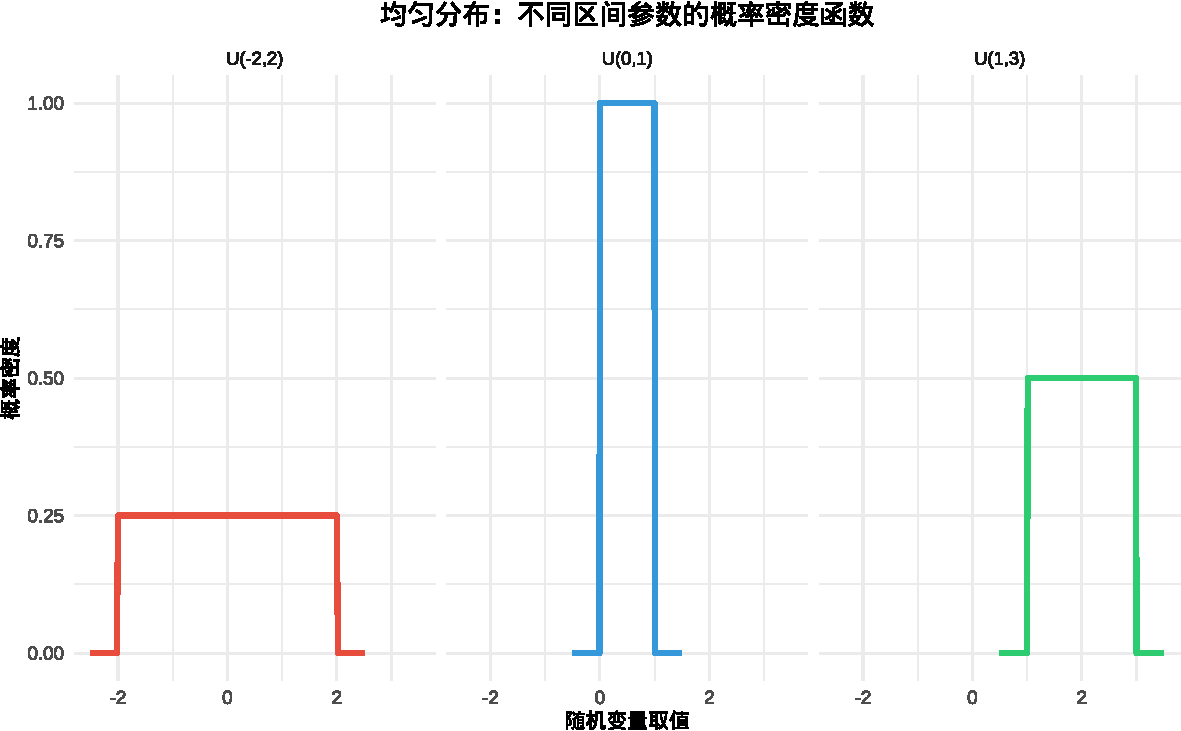
\includegraphics{02-probability_and_distribution_files/figure-latex/unnamed-chunk-27-1.pdf}

\hypertarget{ux8d1dux5854ux5206ux5e03ux6bd4ux4f8bux53d8ux91cfux7684ux5929ux7136ux9009ux62e9}{%
\subsection{贝塔分布:比例变量的天然选择}\label{ux8d1dux5854ux5206ux5e03ux6bd4ux4f8bux53d8ux91cfux7684ux5929ux7136ux9009ux62e9}}

\textbf{故事引入:} 在蚱蜢的日常生活中,时间分配是一个重要的生态学问题。这只蚱蜢在一天24小时中,用于觅食(午餐和其他进食)的时间比例是多少?可能是30\%,也可能是60\%,这个比例值总是在0和1之间。贝塔分布是描述这类比例变量的理想选择,它能够灵活地刻画蚱蜢在不同环境条件下时间分配模式的多样性。

\textbf{数学定义:} 贝塔分布的概率密度函数为:

\[f(x) = \frac{x^{\alpha-1}(1-x)^{\beta-1}}{B(\alpha, \beta)}, \quad 0 \leq x \leq 1\]

其中\(\alpha > 0\)和\(\beta > 0\)是形状参数,\(B(\alpha, \beta)\)是贝塔函数。

\textbf{分布特性:}
- 期望值:\(E[X] = \frac{\alpha}{\alpha + \beta}\)
- 方差:\(Var(X) = \frac{\alpha\beta}{(\alpha+\beta)^2(\alpha+\beta+1)}\)
- 分布形状极其灵活,可以呈现U形、J形、钟形等多种形态
- 当\(\alpha = \beta = 1\)时,贝塔分布退化为均匀分布
- 贝塔分布是二项分布和伯努利分布的共轭先验

\textbf{生态学肖像:}
- \textbf{行为时间分配}:蚱蜢一天中用于觅食、休息、警戒等行为的时间比例
- \textbf{资源选择偏好}:蚱蜢对不同植物种类的选择比例可以用贝塔分布建模
- \textbf{能量预算分析}:通过时间分配比例研究蚱蜢的能量摄入与消耗平衡
- \textbf{适应性行为研究}:贝塔分布的灵活性使其适合描述动物在不同环境下的行为调整

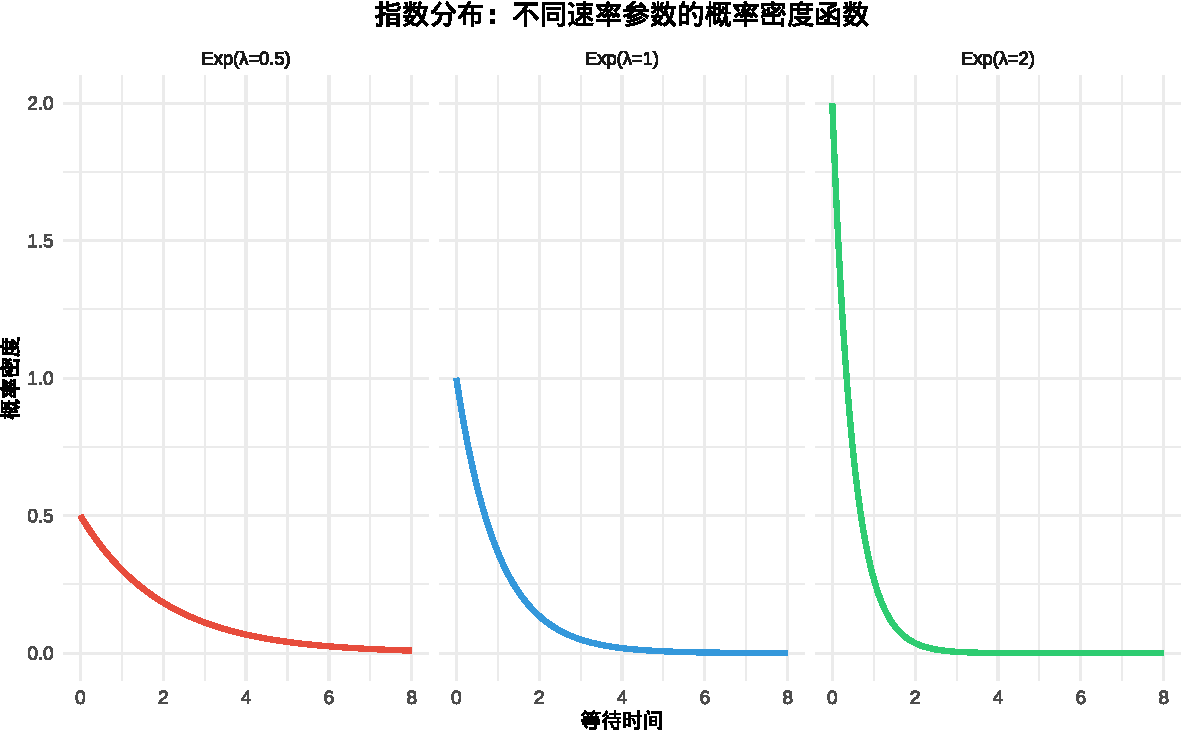
\includegraphics{02-probability_and_distribution_files/figure-latex/unnamed-chunk-28-1.pdf}

\hypertarget{ux6b63ux6001ux7684ux9b54ux529bux4e2dux5fc3ux6781ux9650ux5b9aux7406}{%
\subsection{正态的魔力:中心极限定理}\label{ux6b63ux6001ux7684ux9b54ux529bux4e2dux5fc3ux6781ux9650ux5b9aux7406}}

在我们探索蚱蜢午餐行为的过程中,正态分布以其优雅的钟形曲线给我们留下了深刻印象。但正态分布的真正魔力远不止于此------它拥有一个被称为''统计学的魔法石''的非凡性质:\textbf{中心极限定理}。这个定理解释了为什么正态分布在自然界和统计学中无处不在,即使原始数据本身并不服从正态分布。

\hypertarget{ux4ec0ux4e48ux662fux4e2dux5fc3ux6781ux9650ux5b9aux7406}{%
\subsubsection{什么是中心极限定理}\label{ux4ec0ux4e48ux662fux4e2dux5fc3ux6781ux9650ux5b9aux7406}}

\textbf{中心极限定理}(Central Limit Theorem, CLT)是概率论和统计学中最重要的定理之一。它的核心思想可以概括为:

\begin{quote}
无论原始总体的分布形态如何,只要样本量足够大,样本均值的抽样分布就会近似服从正态分布。
\end{quote}

更精确地说,中心极限定理指出:
- 从任意分布(无论是什么形状)的总体中随机抽取样本
- 计算每个样本的均值
- 当样本量\(n\)足够大时(通常\(n \geq 30\)),这些样本均值的分布将近似正态分布
- 这个正态分布的均值等于总体均值\(\mu\),标准差等于总体标准差\(\sigma\)除以\(\sqrt{n}\)

\textbf{数学表达:}
如果\(X_1, X_2, \ldots, X_n\)是来自均值为\(\mu\)、方差为\(\sigma^2\)的总体的独立同分布随机变量,那么当\(n \to \infty\)时:

\[\frac{\bar{X} - \mu}{\sigma/\sqrt{n}} \xrightarrow{d} N(0, 1)\]

其中\(\bar{X} = \frac{1}{n}\sum_{i=1}^n X_i\)是样本均值,\(\xrightarrow{d}\)表示依分布收敛。

\begin{verbatim}
## 
## Attaching package: 'gridExtra'
\end{verbatim}

\begin{verbatim}
## The following object is masked from 'package:dplyr':
## 
##     combine
\end{verbatim}

\begin{verbatim}
## Warning: The dot-dot notation (`..density..`) was deprecated in ggplot2 3.4.0.
## i Please use `after_stat(density)` instead.
## This warning is displayed once every 8 hours.
## Call `lifecycle::last_lifecycle_warnings()` to see where this warning was generated.
\end{verbatim}

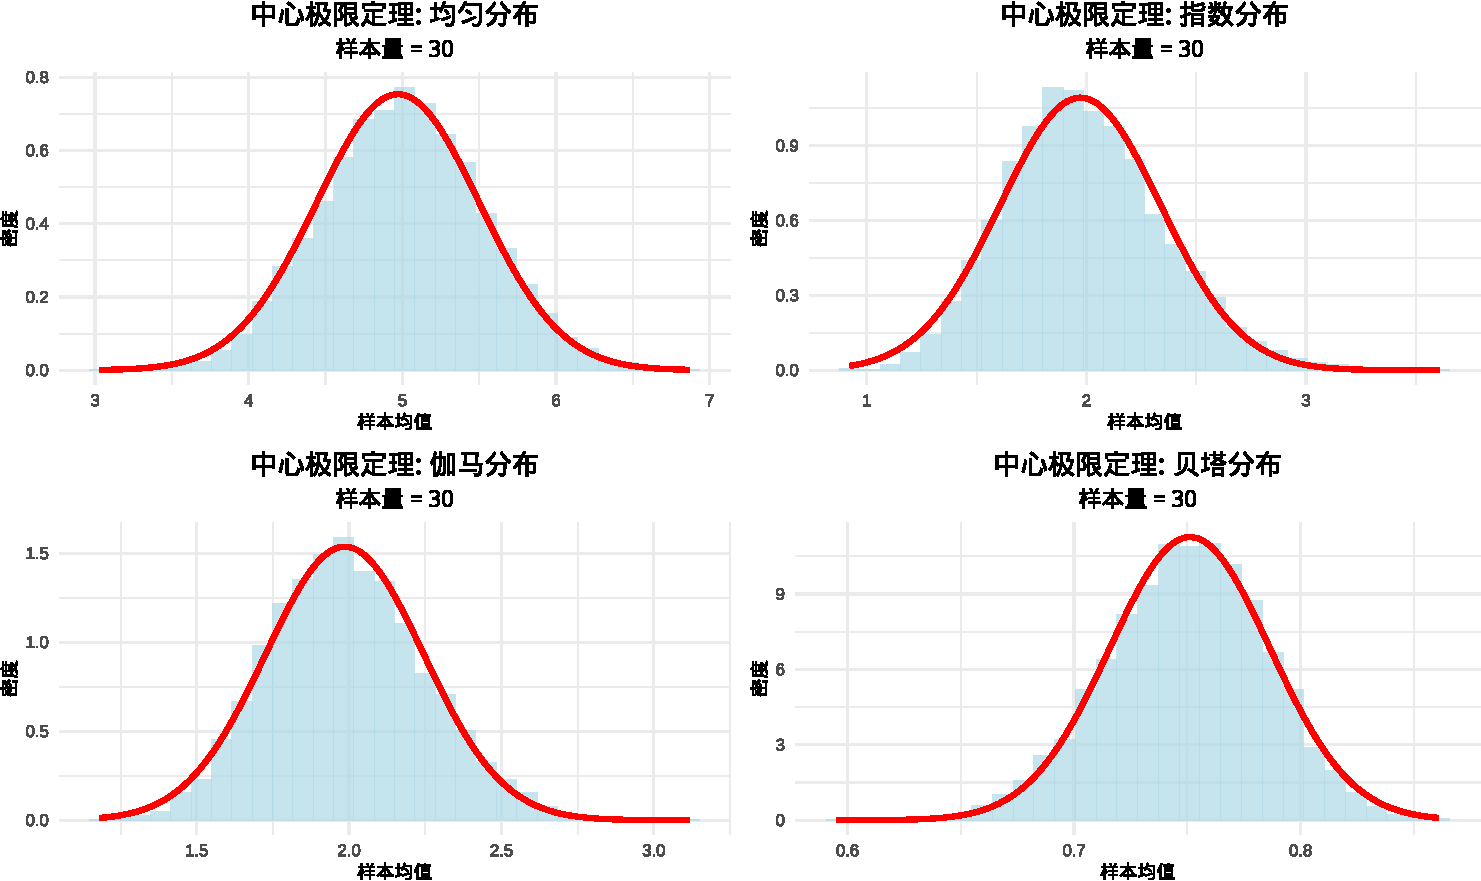
\includegraphics{02-probability_and_distribution_files/figure-latex/unnamed-chunk-29-1.pdf}

\begin{verbatim}
## 中心极限定理正态性检验结果:
\end{verbatim}

\begin{verbatim}
## 均匀分布样本均值Kolmogorov-Smirnov p值: 0.9917
\end{verbatim}

\begin{verbatim}
## 指数分布样本均值Kolmogorov-Smirnov p值: 0
\end{verbatim}

\begin{verbatim}
## 伽马分布样本均值Kolmogorov-Smirnov p值: 0.0014
\end{verbatim}

\begin{verbatim}
## 贝塔分布样本均值Kolmogorov-Smirnov p值: 0.0179
\end{verbatim}

\hypertarget{ux6837ux672cux91cfux5bf9ux4e2dux5fc3ux6781ux9650ux5b9aux7406ux7684ux5f71ux54cd}{%
\subsubsection{样本量对中心极限定理的影响}\label{ux6837ux672cux91cfux5bf9ux4e2dux5fc3ux6781ux9650ux5b9aux7406ux7684ux5f71ux54cd}}

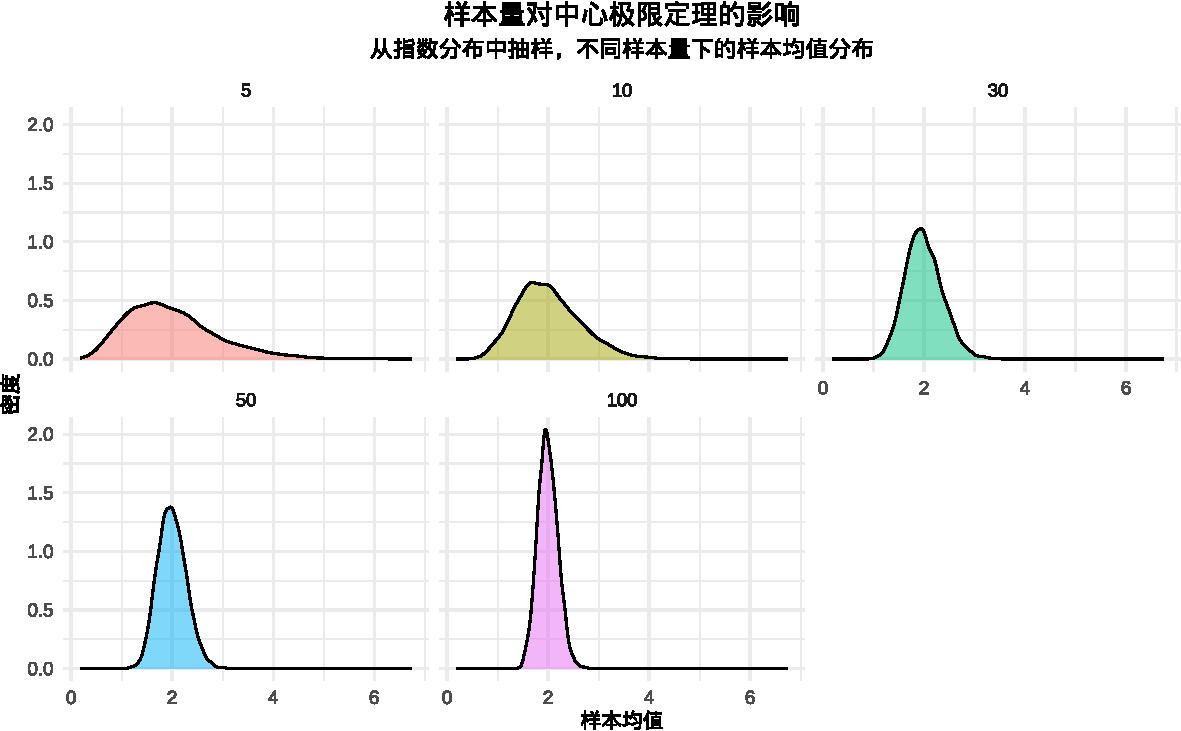
\includegraphics{02-probability_and_distribution_files/figure-latex/unnamed-chunk-30-1.pdf}

\begin{verbatim}
## 偏度和峰度随样本量的变化:
\end{verbatim}

\begin{verbatim}
##   SampleSize  Skewness Kurtosis
## 1          5 0.8974114 4.109759
## 2         10 0.6504552 3.732605
## 3         30 0.4054190 3.315501
## 4         50 0.2691500 3.072610
## 5        100 0.2423726 3.087874
\end{verbatim}

\hypertarget{ux86b1ux8722ux5348ux9910ux4e2dux7684ux4e2dux5fc3ux6781ux9650ux5b9aux7406}{%
\subsubsection{蚱蜢午餐中的中心极限定理}\label{ux86b1ux8722ux5348ux9910ux4e2dux7684ux4e2dux5fc3ux6781ux9650ux5b9aux7406}}

让我们回到蚱蜢的午餐世界,看看中心极限定理如何发挥作用:

\textbf{场景1:摄食量的抽样分布}
假设我们想要了解蚱蜢种群的平均摄食量。单个蚱蜢的摄食量可能呈现各种分布形态------有些蚱蜢吃得少,有些吃得多,分布可能是偏斜的。但是,如果我们随机抽取30只蚱蜢,计算它们的平均摄食量,然后重复这个过程很多次,这些样本均值的分布将呈现完美的钟形曲线!

\textbf{场景2:觅食时间的估计}
蚱蜢的觅食时间可能受到多种因素影响,单个个体的时间分布可能很不规则。但通过中心极限定理,我们可以基于样本均值来可靠地估计整个种群的平均觅食时间。

\textbf{场景3:行为偏好的研究}
即使蚱蜢对植物的选择偏好本身不是正态分布,但当我们研究多个样本的平均偏好时,结果将趋于正态分布。

\hypertarget{ux4e2dux5fc3ux6781ux9650ux5b9aux7406ux7684ux751fux6001ux5b66ux610fux4e49}{%
\subsubsection{中心极限定理的生态学意义}\label{ux4e2dux5fc3ux6781ux9650ux5b9aux7406ux7684ux751fux6001ux5b66ux610fux4e49}}

中心极限定理为生态学研究提供了强大的理论支撑:

\begin{enumerate}
\def\labelenumi{\arabic{enumi}.}
\item
  \textbf{参数估计的可靠性}
  即使我们不知道总体的真实分布,也可以通过样本均值来估计总体参数,而且知道这种估计的误差分布是正态的。
\item
  \textbf{假设检验的基础}
  许多统计检验(如t检验、方差分析)都建立在中心极限定理的基础上,假设样本均值的分布是正态的。
\item
  \textbf{置信区间的构建}
  基于中心极限定理,我们可以构建总体均值的置信区间,为生态学推断提供量化依据。
\item
  \textbf{大样本理论的基石}
  中心极限定理是许多大样本统计方法的基础,使得我们能够在样本量足够时做出可靠的统计推断。
\end{enumerate}

\hypertarget{ux4e2dux5fc3ux6781ux9650ux5b9aux7406ux7684ux5c40ux9650ux6027}{%
\subsubsection{中心极限定理的局限性}\label{ux4e2dux5fc3ux6781ux9650ux5b9aux7406ux7684ux5c40ux9650ux6027}}

尽管中心极限定理非常强大,但在应用时也需要注意其局限性:

\begin{enumerate}
\def\labelenumi{\arabic{enumi}.}
\item
  \textbf{样本量要求}
  定理要求样本量足够大(通常\(n \geq 30\)),对于小样本情况,近似效果可能不佳。
\item
  \textbf{独立性假设}
  样本必须是独立同分布的,如果存在空间自相关或时间序列依赖,定理可能不适用。
\item
  \textbf{方差有限性}
  总体方差必须是有限的,对于方差无限的重尾分布,中心极限定理可能不成立。
\item
  \textbf{收敛速度}
  不同分布的收敛速度不同,有些分布需要更大的样本量才能达到较好的正态近似。
\end{enumerate}

\hypertarget{ux751fux6001ux5b66ux5e94ux7528ux5b9eux4f8b}{%
\subsection{生态学应用实例}\label{ux751fux6001ux5b66ux5e94ux7528ux5b9eux4f8b}}

\textbf{种群密度估计}
通过在不同样方中计数物种个体数,即使个体分布本身是聚集的(如负二项分布),样本均值的分布仍近似正态,这使得我们能够可靠地估计总体密度。

\textbf{环境梯度研究}
沿着环境梯度(如海拔、温度)测量物种丰富度,即使原始数据呈现复杂模式,样本均值的分布仍趋于正态,便于统计分析和建模。

\textbf{行为生态学实验}
在控制实验中测量动物的行为参数,通过中心极限定理,我们可以基于样本均值进行可靠的统计推断。

\hypertarget{ux603bux7ed3-1}{%
\subsubsection{总结}\label{ux603bux7ed3-1}}

中心极限定理是连接概率论与统计推断的桥梁,它解释了为什么正态分布在统计学中占据核心地位。在蚱蜢午餐的研究中,这个定理确保了即使面对复杂的生态数据,我们仍然能够使用基于正态分布的统计方法来获得可靠的科学结论。

正如统计学家乔治·博克斯所言:``所有的模型都是错的,但有些是有用的。''中心极限定理正是这样一个''有用''的模型,它虽然不是绝对精确,但在大多数实际情况下提供了足够好的近似,为生态学的定量研究奠定了坚实的数学基础。

\hypertarget{ux6df7ux5408ux5206ux5e03ux5904ux7406ux5f02ux8d28ux6027ux6570ux636e}{%
\section{混合分布:处理异质性数据}\label{ux6df7ux5408ux5206ux5e03ux5904ux7406ux5f02ux8d28ux6027ux6570ux636e}}

混合分布能够描述来自不同子总体的数据,在生态学中处理异质性非常有用。

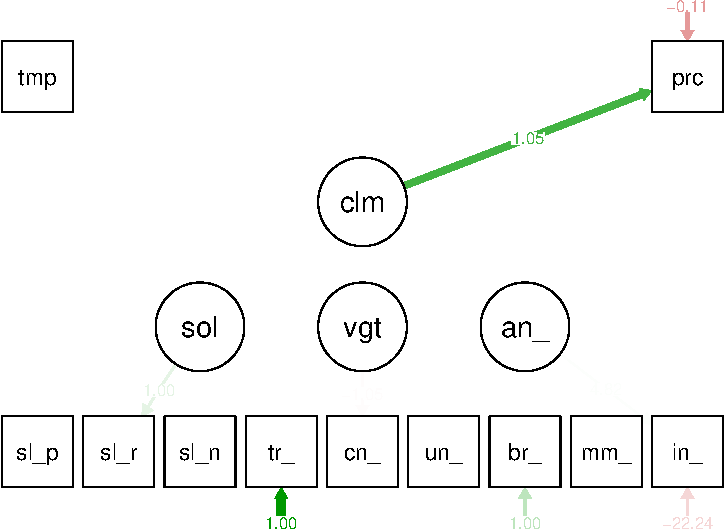
\includegraphics{02-probability_and_distribution_files/figure-latex/unnamed-chunk-31-1.pdf}

\begin{verbatim}
## 混合分布的生态学应用:
\end{verbatim}

\begin{verbatim}
## 1. 不同年龄组的种群结构
\end{verbatim}

\begin{verbatim}
## 2. 异质环境中的物种分布
\end{verbatim}

\begin{verbatim}
## 3. 多物种混合的群落数据
\end{verbatim}

\begin{verbatim}
## 4. 季节性变化的环境因子
\end{verbatim}

\hypertarget{ux96f6ux81a8ux80c0ux5206ux5e03ux5904ux7406ux96f6ux503cux8fc7ux591aux7684ux6570ux636e}{%
\subsection{零膨胀分布:处理零值过多的数据}\label{ux96f6ux81a8ux80c0ux5206ux5e03ux5904ux7406ux96f6ux503cux8fc7ux591aux7684ux6570ux636e}}

在生态学中,许多计数数据存在大量的零值,零膨胀分布专门处理这类数据。

\begin{Shaded}
\begin{Highlighting}[]
\CommentTok{\# 零膨胀分布概念演示}
\FunctionTok{set.seed}\NormalTok{(}\DecValTok{2323}\NormalTok{)}

\CommentTok{\# 模拟零膨胀数据:80\%的零值和20\%的泊松分布}
\NormalTok{n\_samples }\OtherTok{\textless{}{-}} \DecValTok{1000}
\NormalTok{zero\_prob }\OtherTok{\textless{}{-}} \FloatTok{0.8}
\NormalTok{lambda }\OtherTok{\textless{}{-}} \DecValTok{3}

\CommentTok{\# 生成零膨胀泊松数据}
\NormalTok{zip\_data }\OtherTok{\textless{}{-}} \FunctionTok{numeric}\NormalTok{(n\_samples)}
\ControlFlowTok{for}\NormalTok{ (i }\ControlFlowTok{in} \DecValTok{1}\SpecialCharTok{:}\NormalTok{n\_samples) \{}
  \ControlFlowTok{if}\NormalTok{ (}\FunctionTok{runif}\NormalTok{(}\DecValTok{1}\NormalTok{) }\SpecialCharTok{\textless{}}\NormalTok{ zero\_prob) \{}
\NormalTok{    zip\_data[i] }\OtherTok{\textless{}{-}} \DecValTok{0}
\NormalTok{  \} }\ControlFlowTok{else}\NormalTok{ \{}
\NormalTok{    zip\_data[i] }\OtherTok{\textless{}{-}} \FunctionTok{rpois}\NormalTok{(}\DecValTok{1}\NormalTok{, lambda)}
\NormalTok{  \}}
\NormalTok{\}}

\CommentTok{\# 统计零值比例}
\NormalTok{zero\_proportion }\OtherTok{\textless{}{-}} \FunctionTok{mean}\NormalTok{(zip\_data }\SpecialCharTok{==} \DecValTok{0}\NormalTok{)}
\FunctionTok{cat}\NormalTok{(}\StringTok{"零膨胀数据统计:}\SpecialCharTok{\textbackslash{}n}\StringTok{"}\NormalTok{)}
\end{Highlighting}
\end{Shaded}

\begin{verbatim}
## 零膨胀数据统计:
\end{verbatim}

\begin{Shaded}
\begin{Highlighting}[]
\FunctionTok{cat}\NormalTok{(}\StringTok{"零值比例:"}\NormalTok{, }\FunctionTok{round}\NormalTok{(zero\_proportion, }\DecValTok{3}\NormalTok{), }\StringTok{"}\SpecialCharTok{\textbackslash{}n}\StringTok{"}\NormalTok{)}
\end{Highlighting}
\end{Shaded}

\begin{verbatim}
## 零值比例: 0.793
\end{verbatim}

\begin{Shaded}
\begin{Highlighting}[]
\FunctionTok{cat}\NormalTok{(}\StringTok{"非零值均值:"}\NormalTok{, }\FunctionTok{round}\NormalTok{(}\FunctionTok{mean}\NormalTok{(zip\_data[zip\_data }\SpecialCharTok{\textgreater{}} \DecValTok{0}\NormalTok{]), }\DecValTok{3}\NormalTok{), }\StringTok{"}\SpecialCharTok{\textbackslash{}n}\StringTok{"}\NormalTok{)}
\end{Highlighting}
\end{Shaded}

\begin{verbatim}
## 非零值均值: 3.266
\end{verbatim}

\begin{Shaded}
\begin{Highlighting}[]
\FunctionTok{cat}\NormalTok{(}\StringTok{"总体均值:"}\NormalTok{, }\FunctionTok{round}\NormalTok{(}\FunctionTok{mean}\NormalTok{(zip\_data), }\DecValTok{3}\NormalTok{), }\StringTok{"}\SpecialCharTok{\textbackslash{}n}\StringTok{"}\NormalTok{)}
\end{Highlighting}
\end{Shaded}

\begin{verbatim}
## 总体均值: 0.676
\end{verbatim}

\begin{Shaded}
\begin{Highlighting}[]
\CommentTok{\# 与普通泊松分布比较}
\NormalTok{poisson\_data }\OtherTok{\textless{}{-}} \FunctionTok{rpois}\NormalTok{(n\_samples, }\AttributeTok{lambda =} \FunctionTok{mean}\NormalTok{(zip\_data))}
\FunctionTok{cat}\NormalTok{(}\StringTok{"}\SpecialCharTok{\textbackslash{}n}\StringTok{与普通泊松分布比较:}\SpecialCharTok{\textbackslash{}n}\StringTok{"}\NormalTok{)}
\end{Highlighting}
\end{Shaded}

\begin{verbatim}
## 
## 与普通泊松分布比较:
\end{verbatim}

\begin{Shaded}
\begin{Highlighting}[]
\FunctionTok{cat}\NormalTok{(}\StringTok{"泊松零值比例:"}\NormalTok{, }\FunctionTok{round}\NormalTok{(}\FunctionTok{mean}\NormalTok{(poisson\_data }\SpecialCharTok{==} \DecValTok{0}\NormalTok{), }\DecValTok{3}\NormalTok{), }\StringTok{"}\SpecialCharTok{\textbackslash{}n}\StringTok{"}\NormalTok{)}
\end{Highlighting}
\end{Shaded}

\begin{verbatim}
## 泊松零值比例: 0.534
\end{verbatim}

\begin{Shaded}
\begin{Highlighting}[]
\FunctionTok{cat}\NormalTok{(}\StringTok{"泊松方差:"}\NormalTok{, }\FunctionTok{round}\NormalTok{(}\FunctionTok{var}\NormalTok{(poisson\_data), }\DecValTok{3}\NormalTok{), }\StringTok{"}\SpecialCharTok{\textbackslash{}n}\StringTok{"}\NormalTok{)}
\end{Highlighting}
\end{Shaded}

\begin{verbatim}
## 泊松方差: 0.657
\end{verbatim}

\begin{Shaded}
\begin{Highlighting}[]
\FunctionTok{cat}\NormalTok{(}\StringTok{"零膨胀方差:"}\NormalTok{, }\FunctionTok{round}\NormalTok{(}\FunctionTok{var}\NormalTok{(zip\_data), }\DecValTok{3}\NormalTok{), }\StringTok{"}\SpecialCharTok{\textbackslash{}n}\StringTok{"}\NormalTok{)}
\end{Highlighting}
\end{Shaded}

\begin{verbatim}
## 零膨胀方差: 2.361
\end{verbatim}

\begin{Shaded}
\begin{Highlighting}[]
\FunctionTok{cat}\NormalTok{(}\StringTok{"过度分散指数:"}\NormalTok{, }\FunctionTok{round}\NormalTok{(}\FunctionTok{var}\NormalTok{(zip\_data)}\SpecialCharTok{/}\FunctionTok{mean}\NormalTok{(zip\_data), }\DecValTok{3}\NormalTok{), }\StringTok{"}\SpecialCharTok{\textbackslash{}n}\StringTok{"}\NormalTok{)}
\end{Highlighting}
\end{Shaded}

\begin{verbatim}
## 过度分散指数: 3.493
\end{verbatim}

\begin{Shaded}
\begin{Highlighting}[]
\CommentTok{\# 零膨胀分布的生态学意义}
\FunctionTok{cat}\NormalTok{(}\StringTok{"}\SpecialCharTok{\textbackslash{}n}\StringTok{零膨胀分布的生态学应用:}\SpecialCharTok{\textbackslash{}n}\StringTok{"}\NormalTok{)}
\end{Highlighting}
\end{Shaded}

\begin{verbatim}
## 
## 零膨胀分布的生态学应用:
\end{verbatim}

\begin{Shaded}
\begin{Highlighting}[]
\FunctionTok{cat}\NormalTok{(}\StringTok{"1. 稀有物种的出现数据}\SpecialCharTok{\textbackslash{}n}\StringTok{"}\NormalTok{)}
\end{Highlighting}
\end{Shaded}

\begin{verbatim}
## 1. 稀有物种的出现数据
\end{verbatim}

\begin{Shaded}
\begin{Highlighting}[]
\FunctionTok{cat}\NormalTok{(}\StringTok{"2. 低密度种群的分布数据}\SpecialCharTok{\textbackslash{}n}\StringTok{"}\NormalTok{)}
\end{Highlighting}
\end{Shaded}

\begin{verbatim}
## 2. 低密度种群的分布数据
\end{verbatim}

\begin{Shaded}
\begin{Highlighting}[]
\FunctionTok{cat}\NormalTok{(}\StringTok{"3. 间歇性生态过程记录}\SpecialCharTok{\textbackslash{}n}\StringTok{"}\NormalTok{)}
\end{Highlighting}
\end{Shaded}

\begin{verbatim}
## 3. 间歇性生态过程记录
\end{verbatim}

\begin{Shaded}
\begin{Highlighting}[]
\FunctionTok{cat}\NormalTok{(}\StringTok{"4. 不完全调查的观测数据}\SpecialCharTok{\textbackslash{}n}\StringTok{"}\NormalTok{)}
\end{Highlighting}
\end{Shaded}

\begin{verbatim}
## 4. 不完全调查的观测数据
\end{verbatim}

\hypertarget{ux9644ux5f551-rux8bedux8a00ux7f16ux7a0bux57faux7840}{%
\chapter{附录1 R语言编程基础}\label{ux9644ux5f551-rux8bedux8a00ux7f16ux7a0bux57faux7840}}

\hypertarget{rux8bedux8a00ux4ecbux7ecd}{%
\section{R语言介绍}\label{rux8bedux8a00ux4ecbux7ecd}}

\begin{itemize}
\tightlist
\item
  理解为什么生态学专业需要学习R语言
\item
  掌握R和RStudio的安装和配置
\item
  建立良好的项目文件组织习惯
\item
  了解R包管理的基本方法
\end{itemize}

\hypertarget{ux4e3aux4ec0ux4e48ux751fux6001ux5b66ux4e13ux4e1aux9700ux8981ux5b66ux4e60r}{%
\subsection{为什么生态学专业需要学习R?}\label{ux4e3aux4ec0ux4e48ux751fux6001ux5b66ux4e13ux4e1aux9700ux8981ux5b66ux4e60r}}

\hypertarget{ux6570ux636eux5206ux6790ux80fdux529bux7684ux5fc5ux8981ux6027}{%
\subsubsection{数据分析能力的必要性}\label{ux6570ux636eux5206ux6790ux80fdux529bux7684ux5fc5ux8981ux6027}}

现代生态学研究产生海量数据:野外调查数据、实验室测量数据、遥感影像数据、基因序列数据等。传统的Excel已无法满足复杂的统计分析需求,而R语言提供了完整的数据科学工具链。

\hypertarget{ux53efux91cdux73b0ux7814ux7a76ux7684ux79d1ux5b66ux8981ux6c42}{%
\subsubsection{可重现研究的科学要求}\label{ux53efux91cdux73b0ux7814ux7a76ux7684ux79d1ux5b66ux8981ux6c42}}

\begin{itemize}
\tightlist
\item
  \textbf{重现性危机}:越来越多的科学研究无法被重现,影响科学可信度
\item
  \textbf{R脚本的优势}:

  \begin{itemize}
  \tightlist
  \item
    每一步分析都有记录,任何人都可以重现你的分析过程
  \item
    错误检查:代码可以被审查,减少人为错误
  \item
    版本控制:分析过程的每次修改都有记录
  \end{itemize}
\end{itemize}

\hypertarget{ux804cux4e1aux53d1ux5c55ux7684ux6838ux5fc3ux7adeux4e89ux529b}{%
\subsubsection{职业发展的核心竞争力}\label{ux804cux4e1aux53d1ux5c55ux7684ux6838ux5fc3ux7adeux4e89ux529b}}

\begin{itemize}
\tightlist
\item
  \textbf{学术界要求}:顶级期刊越来越要求提供数据和代码
\item
  \textbf{就业市场需求}:环保部门、研究院所、咨询公司都需要数据分析能力
\item
  \textbf{跨学科合作}:与计算机科学、统计学等领域合作的桥梁
\item
  \textbf{终身学习}:编程思维有助于快速学习新的分析方法
\end{itemize}

\hypertarget{ux5f00ux6e90ux514dux8d39ux7684ux7ecfux6d4eux4f18ux52bf}{%
\subsubsection{开源免费的经济优势}\label{ux5f00ux6e90ux514dux8d39ux7684ux7ecfux6d4eux4f18ux52bf}}

\begin{itemize}
\tightlist
\item
  \textbf{成本优势}:SPSS单机版数万元,SAS更昂贵,R完全免费
\item
  \textbf{功能更新}:商业软件更新缓慢,R社区每天都有新功能
\item
  \textbf{全球社区}:遇到问题可以在全球社区寻求帮助
\item
  \textbf{未来保障}:开源软件不会因为公司倒闭而消失
\end{itemize}

\hypertarget{ux5b66ux672fux53d1ux8868ux7684ux5fc5ux8981ux5de5ux5177}{%
\subsubsection{学术发表的必要工具}\label{ux5b66ux672fux53d1ux8868ux7684ux5fc5ux8981ux5de5ux5177}}

\begin{itemize}
\tightlist
\item
  \textbf{期刊要求}:Nature、Science等顶级期刊要求提供分析代码
\item
  \textbf{同行评议}:审稿人可以检查你的分析方法是否正确
\item
  \textbf{引用优势}:提供代码的论文被引用次数更高
\item
  \textbf{学术诚信}:透明的分析过程展现严谨的科学态度
\end{itemize}

\hypertarget{ux56fdux9645ux4ea4ux6d41ux7684ux901aux7528ux8bedux8a00}{%
\subsubsection{国际交流的通用语言}\label{ux56fdux9645ux4ea4ux6d41ux7684ux901aux7528ux8bedux8a00}}

\begin{itemize}
\tightlist
\item
  \textbf{国际会议}:生态学国际会议上,R是数据分析的主流工具
\item
  \textbf{合作研究}:与国外学者合作时,R是共同的工作语言
\item
  \textbf{在线学习}:全球最优秀的生态学分析教程都使用R
\item
  \textbf{职业流动}:掌握R可以在全球范围内寻求工作机会
\end{itemize}

\hypertarget{rux8bedux8a00ux7b80ux4ecbux4e0eux8da3ux5473ux5e94ux7528}{%
\subsection{R语言简介与趣味应用}\label{rux8bedux8a00ux7b80ux4ecbux4e0eux8da3ux5473ux5e94ux7528}}

\hypertarget{ux4ec0ux4e48ux662frux8bedux8a00}{%
\subsubsection{什么是R语言?}\label{ux4ec0ux4e48ux662frux8bedux8a00}}

\begin{itemize}
\tightlist
\item
  \textbf{统计计算语言}:专门为统计分析和数据可视化设计的编程语言
\item
  \textbf{开源免费}:由全球统计学家共同维护发展
\item
  \textbf{交互式环境}:可以立即看到代码执行结果
\item
  \textbf{扩展性强}:超过18,000个专业扩展包
\end{itemize}

\hypertarget{ux5982ux4f55ux83b7ux53d6ux5e2eux52a9}{%
\subsubsection{如何获取帮助?}\label{ux5982ux4f55ux83b7ux53d6ux5e2eux52a9}}

\begin{Shaded}
\begin{Highlighting}[]
\CommentTok{\# 查看函数帮助文档}
\NormalTok{?plot}
\FunctionTok{help}\NormalTok{(}\StringTok{"plot"}\NormalTok{)}

\CommentTok{\# 搜索帮助文档}
\NormalTok{??}\StringTok{"regression"}

\CommentTok{\# 示例代码演示}
\FunctionTok{example}\NormalTok{(plot)}
\FunctionTok{example}\NormalTok{(lm)}
\FunctionTok{demo}\NormalTok{(persp)}
\FunctionTok{demo}\NormalTok{(graphics)}
\FunctionTok{demo}\NormalTok{(Hershey)}
\FunctionTok{demo}\NormalTok{(plotmath)}


\CommentTok{\# 在线资源:}
\CommentTok{\# {-} R官方文档:https://cran.r{-}project.org/manuals.html}
\CommentTok{\# {-} RStudio社区:https://community.rstudio.com}
\end{Highlighting}
\end{Shaded}

\hypertarget{rux8bedux8a00ux7684ux8da3ux5473ux5e94ux7528ux793aux4f8b}{%
\subsubsection{R语言的趣味应用示例}\label{rux8bedux8a00ux7684ux8da3ux5473ux5e94ux7528ux793aux4f8b}}

\hypertarget{ux751fux6001ux6570ux636eux52a8ux6001ux53efux89c6ux5316}{%
\paragraph{生态数据动态可视化}\label{ux751fux6001ux6570ux636eux52a8ux6001ux53efux89c6ux5316}}

\begin{Shaded}
\begin{Highlighting}[]
\CommentTok{\# 安装必要包(首次需要)}
\FunctionTok{install.packages}\NormalTok{(}\FunctionTok{c}\NormalTok{(}\StringTok{"ggplot2"}\NormalTok{, }\StringTok{"gganimate"}\NormalTok{, }\StringTok{"gapminder"}\NormalTok{))}
\FunctionTok{library}\NormalTok{(ggplot2)}
\FunctionTok{library}\NormalTok{(gganimate)}
\FunctionTok{library}\NormalTok{(gapminder)}

\CommentTok{\# 使用gapminder数据集(包含各国多年生态经济数据)}
\CommentTok{\# 绘制动态变化图}
\NormalTok{fig }\OtherTok{\textless{}{-}} \FunctionTok{ggplot}\NormalTok{(gapminder, }\FunctionTok{aes}\NormalTok{(gdpPercap, lifeExp, }\AttributeTok{size =}\NormalTok{ pop, }\AttributeTok{color =}\NormalTok{ continent)) }\SpecialCharTok{+}
  \FunctionTok{geom\_point}\NormalTok{() }\SpecialCharTok{+}
  \FunctionTok{scale\_size}\NormalTok{(}\AttributeTok{range =} \FunctionTok{c}\NormalTok{(}\DecValTok{2}\NormalTok{, }\DecValTok{12}\NormalTok{)) }\SpecialCharTok{+}
  \FunctionTok{scale\_x\_log10}\NormalTok{() }\SpecialCharTok{+}
  \FunctionTok{labs}\NormalTok{(}\AttributeTok{title =} \StringTok{\textquotesingle{}年份: \{frame\_time\}\textquotesingle{}}\NormalTok{, }\AttributeTok{x =} \StringTok{\textquotesingle{}人均GDP\textquotesingle{}}\NormalTok{, }\AttributeTok{y =} \StringTok{\textquotesingle{}预期寿命\textquotesingle{}}\NormalTok{) }\SpecialCharTok{+}
  \FunctionTok{transition\_time}\NormalTok{(year) }\SpecialCharTok{+}
  \FunctionTok{ease\_aes}\NormalTok{(}\StringTok{\textquotesingle{}linear\textquotesingle{}}\NormalTok{)}

\CommentTok{\# 渲染并保存动画}
\CommentTok{\# 需要先安装gifski包: install.packages("gifski")}
\FunctionTok{animate}\NormalTok{(fig, }\AttributeTok{renderer =} \FunctionTok{gifski\_renderer}\NormalTok{(}\StringTok{"./imgs/gapminder\_animation.gif"}\NormalTok{), }
        \AttributeTok{width =} \DecValTok{800}\NormalTok{, }\AttributeTok{height =} \DecValTok{600}\NormalTok{, }\AttributeTok{fps =} \DecValTok{10}\NormalTok{, }\AttributeTok{duration =} \DecValTok{15}\NormalTok{)}

\CommentTok{\# 提示:运行后会生成展示生态经济数据随时间变化的动画}
\CommentTok{\# 可以清楚地看到不同大陆国家生态经济指标的变化趋势}
\end{Highlighting}
\end{Shaded}

\hypertarget{ux7535ux5b50ux6c34ux6bcd}{%
\subsubsection{电子水母}\label{ux7535ux5b50ux6c34ux6bcd}}

\begin{Shaded}
\begin{Highlighting}[]
\CommentTok{\# 加载必要的包}
\FunctionTok{library}\NormalTok{(ggplot2)}
\FunctionTok{library}\NormalTok{(gganimate) }\CommentTok{\# 用于创建动画}
\FunctionTok{library}\NormalTok{(dplyr)     }\CommentTok{\# 用于数据处理}

\CommentTok{\# 设置参数 {-} 减少点数提高性能}
\NormalTok{i }\OtherTok{\textless{}{-}} \DecValTok{0}\SpecialCharTok{:}\DecValTok{2000}  \CommentTok{\# 从10000减少到2000个点}
\NormalTok{x }\OtherTok{\textless{}{-}}\NormalTok{ i }\SpecialCharTok{\%\%} \DecValTok{200}      \CommentTok{\# R中的模运算}
\NormalTok{y }\OtherTok{\textless{}{-}}\NormalTok{ i }\SpecialCharTok{/} \DecValTok{43}

\CommentTok{\# 预计算固定变量(不依赖于t)}
\NormalTok{k }\OtherTok{\textless{}{-}} \DecValTok{5} \SpecialCharTok{*} \FunctionTok{cos}\NormalTok{(x}\SpecialCharTok{/}\DecValTok{14}\NormalTok{) }\SpecialCharTok{*} \FunctionTok{cos}\NormalTok{(y}\SpecialCharTok{/}\DecValTok{30}\NormalTok{)}
\NormalTok{e }\OtherTok{\textless{}{-}}\NormalTok{ y}\SpecialCharTok{/}\DecValTok{8} \SpecialCharTok{{-}} \DecValTok{13}
\NormalTok{d }\OtherTok{\textless{}{-}}\NormalTok{ (k}\SpecialCharTok{\^{}}\DecValTok{2} \SpecialCharTok{+}\NormalTok{ e}\SpecialCharTok{\^{}}\DecValTok{2}\NormalTok{)}\SpecialCharTok{/}\DecValTok{59} \SpecialCharTok{+} \DecValTok{4}
\NormalTok{a }\OtherTok{\textless{}{-}} \FunctionTok{atan2}\NormalTok{(k, e)   }\CommentTok{\# 注意R中atan2的参数顺序是(y,x)}

\CommentTok{\# 预计算所有帧数据(向量化操作)}
\NormalTok{t\_values }\OtherTok{\textless{}{-}} \FunctionTok{seq}\NormalTok{(}\DecValTok{0}\NormalTok{, }\DecValTok{10} \SpecialCharTok{*}\NormalTok{ pi, }\AttributeTok{by =}\NormalTok{ pi }\SpecialCharTok{/} \DecValTok{10}\NormalTok{)  }\CommentTok{\# 减少帧数:从20π到10π,步长从π/20到π/10}

\CommentTok{\# 使用矩阵运算代替循环}
\NormalTok{c\_val\_matrix }\OtherTok{\textless{}{-}} \FunctionTok{outer}\NormalTok{(d }\SpecialCharTok{/} \DecValTok{2} \SpecialCharTok{+}\NormalTok{ e }\SpecialCharTok{/} \DecValTok{99}\NormalTok{, }\SpecialCharTok{{-}}\NormalTok{t\_values }\SpecialCharTok{/} \DecValTok{18}\NormalTok{, }\StringTok{"+"}\NormalTok{)}
\NormalTok{q\_matrix }\OtherTok{\textless{}{-}} \DecValTok{60} \SpecialCharTok{{-}} \DecValTok{3} \SpecialCharTok{*} \FunctionTok{sin}\NormalTok{(a }\SpecialCharTok{*}\NormalTok{ e) }\SpecialCharTok{+} \FunctionTok{outer}\NormalTok{(k }\SpecialCharTok{*}\NormalTok{ (}\DecValTok{3} \SpecialCharTok{+} \DecValTok{4} \SpecialCharTok{/}\NormalTok{ d), }\FunctionTok{sin}\NormalTok{(d }\SpecialCharTok{\^{}} \DecValTok{2} \SpecialCharTok{{-}} \DecValTok{2} \SpecialCharTok{*}\NormalTok{ t\_values), }\StringTok{"*"}\NormalTok{)}

\NormalTok{x\_matrix }\OtherTok{\textless{}{-}}\NormalTok{ q\_matrix }\SpecialCharTok{*} \FunctionTok{sin}\NormalTok{(c\_val\_matrix) }\SpecialCharTok{+} \DecValTok{200}
\NormalTok{y\_matrix }\OtherTok{\textless{}{-}}\NormalTok{ (q\_matrix }\SpecialCharTok{+} \DecValTok{9} \SpecialCharTok{*}\NormalTok{ d) }\SpecialCharTok{*} \FunctionTok{cos}\NormalTok{(c\_val\_matrix) }\SpecialCharTok{+} \DecValTok{200}

\CommentTok{\# 创建数据框(更高效的方式)}
\NormalTok{all\_frames }\OtherTok{\textless{}{-}} \FunctionTok{data.frame}\NormalTok{(}
  \AttributeTok{t =} \FunctionTok{rep}\NormalTok{(t\_values, }\AttributeTok{each =} \FunctionTok{length}\NormalTok{(i)),}
  \AttributeTok{X =} \FunctionTok{as.vector}\NormalTok{(x\_matrix),}
  \AttributeTok{Y =} \FunctionTok{as.vector}\NormalTok{(y\_matrix)}
\NormalTok{)}

\CommentTok{\# 创建动画}
\NormalTok{anim }\OtherTok{\textless{}{-}} \FunctionTok{ggplot}\NormalTok{(all\_frames, }\FunctionTok{aes}\NormalTok{(X, Y)) }\SpecialCharTok{+}
  \FunctionTok{geom\_point}\NormalTok{(}\AttributeTok{size =} \FloatTok{0.2}\NormalTok{, }\AttributeTok{alpha =} \FloatTok{0.2}\NormalTok{, }\AttributeTok{color =} \StringTok{"white"}\NormalTok{) }\SpecialCharTok{+}
  \FunctionTok{theme\_void}\NormalTok{() }\SpecialCharTok{+}
  \FunctionTok{theme}\NormalTok{(}\AttributeTok{plot.background =} \FunctionTok{element\_rect}\NormalTok{(}\AttributeTok{fill =} \StringTok{"black"}\NormalTok{, }\AttributeTok{color =} \ConstantTok{NA}\NormalTok{),}
        \AttributeTok{panel.background =} \FunctionTok{element\_rect}\NormalTok{(}\AttributeTok{fill =} \StringTok{"black"}\NormalTok{, }\AttributeTok{color =} \ConstantTok{NA}\NormalTok{)) }\SpecialCharTok{+}
  \FunctionTok{coord\_cartesian}\NormalTok{(}\AttributeTok{xlim =} \FunctionTok{c}\NormalTok{(}\DecValTok{0}\NormalTok{, }\DecValTok{400}\NormalTok{), }\AttributeTok{ylim =} \FunctionTok{c}\NormalTok{(}\DecValTok{0}\NormalTok{, }\DecValTok{400}\NormalTok{)) }\SpecialCharTok{+}
  \FunctionTok{transition\_time}\NormalTok{(t) }\SpecialCharTok{+}
  \FunctionTok{shadow\_mark}\NormalTok{(}\AttributeTok{past =} \ConstantTok{FALSE}\NormalTok{, }\AttributeTok{alpha =} \FloatTok{0.05}\NormalTok{)  }\CommentTok{\# 保留轨迹痕迹}

\CommentTok{\# 渲染动画(可能需要几分钟时间)}
\FunctionTok{animate}\NormalTok{(anim, }
        \AttributeTok{fps =} \DecValTok{20}\NormalTok{, }
        \AttributeTok{duration =} \DecValTok{30}\NormalTok{, }
        \AttributeTok{width =} \DecValTok{900}\NormalTok{, }
        \AttributeTok{height =} \DecValTok{900}\NormalTok{,}
        \AttributeTok{renderer =} \FunctionTok{gifski\_renderer}\NormalTok{())}

\CommentTok{\# 保存动画(可选)}
\CommentTok{\# anim\_save("animation.gif", animation = last\_animation())}
\end{Highlighting}
\end{Shaded}

\hypertarget{ux751fux6210ux97f3ux4e50}{%
\paragraph{生成音乐}\label{ux751fux6210ux97f3ux4e50}}

\begin{Shaded}
\begin{Highlighting}[]
\FunctionTok{install.packages}\NormalTok{(}\StringTok{"audio"}\NormalTok{)}
\FunctionTok{install.packages}\NormalTok{(}\StringTok{"dplyr"}\NormalTok{)}
\FunctionTok{library}\NormalTok{(audio)}
\FunctionTok{library}\NormalTok{(dplyr)}
\NormalTok{notes }\OtherTok{\textless{}{-}} \FunctionTok{c}\NormalTok{(}\AttributeTok{A =} \DecValTok{0}\NormalTok{, }\AttributeTok{B =} \DecValTok{2}\NormalTok{, }\AttributeTok{C =} \DecValTok{3}\NormalTok{, }\AttributeTok{D =} \DecValTok{5}\NormalTok{, }\AttributeTok{E =} \DecValTok{7}\NormalTok{, }\AttributeTok{F =} \DecValTok{8}\NormalTok{, }\AttributeTok{G =} \DecValTok{10}\NormalTok{)}
\NormalTok{pitch }\OtherTok{\textless{}{-}} \StringTok{"D D E D G F\# D D E D A G D D D5 B G F\# E C5 C5 B G A G"}
\NormalTok{duration }\OtherTok{\textless{}{-}} \FunctionTok{c}\NormalTok{(}\FunctionTok{rep}\NormalTok{(}\FunctionTok{c}\NormalTok{(}\FloatTok{0.75}\NormalTok{, }\FloatTok{0.25}\NormalTok{, }\DecValTok{1}\NormalTok{, }\DecValTok{1}\NormalTok{, }\DecValTok{1}\NormalTok{, }\DecValTok{2}\NormalTok{), }\DecValTok{2}\NormalTok{),}
              \FloatTok{0.75}\NormalTok{, }\FloatTok{0.25}\NormalTok{, }\DecValTok{1}\NormalTok{, }\DecValTok{1}\NormalTok{, }\DecValTok{1}\NormalTok{, }\DecValTok{1}\NormalTok{, }\DecValTok{1}\NormalTok{, }\FloatTok{0.75}\NormalTok{, }\FloatTok{0.25}\NormalTok{, }\DecValTok{1}\NormalTok{, }\DecValTok{1}\NormalTok{, }\DecValTok{1}\NormalTok{, }\DecValTok{2}\NormalTok{)}
\NormalTok{bday }\OtherTok{\textless{}{-}} \FunctionTok{data\_frame}\NormalTok{(}\AttributeTok{pitch =} \FunctionTok{strsplit}\NormalTok{(pitch, }\StringTok{" "}\NormalTok{)[[}\DecValTok{1}\NormalTok{]],}
                   \AttributeTok{duration =}\NormalTok{ duration)}

\NormalTok{bday }\OtherTok{\textless{}{-}}
\NormalTok{  bday }\SpecialCharTok{\%\textgreater{}\%}
  \FunctionTok{mutate}\NormalTok{(}\AttributeTok{octave =} \FunctionTok{substring}\NormalTok{(pitch, }\FunctionTok{nchar}\NormalTok{(pitch)) }\SpecialCharTok{\%\textgreater{}\%}
\NormalTok{  \{}\FunctionTok{suppressWarnings}\NormalTok{(}\FunctionTok{as.numeric}\NormalTok{(.))\} }\SpecialCharTok{\%\textgreater{}\%}
    \FunctionTok{ifelse}\NormalTok{(}\FunctionTok{is.na}\NormalTok{(.), }\DecValTok{4}\NormalTok{, .),}
  \AttributeTok{note =}\NormalTok{ notes[}\FunctionTok{substr}\NormalTok{(pitch, }\DecValTok{1}\NormalTok{, }\DecValTok{1}\NormalTok{)],}
  \AttributeTok{note =}\NormalTok{ note }\SpecialCharTok{+} \FunctionTok{grepl}\NormalTok{(}\StringTok{"\#"}\NormalTok{, pitch) }\SpecialCharTok{{-}}
    \FunctionTok{grepl}\NormalTok{(}\StringTok{"b"}\NormalTok{, pitch) }\SpecialCharTok{+}\NormalTok{ octave }\SpecialCharTok{*} \DecValTok{12} \SpecialCharTok{+}
    \DecValTok{12} \SpecialCharTok{*}\NormalTok{ (note }\SpecialCharTok{\textless{}} \DecValTok{3}\NormalTok{),}
  \AttributeTok{freq =} \DecValTok{2} \SpecialCharTok{\^{}}\NormalTok{ ((note }\SpecialCharTok{{-}} \DecValTok{60}\NormalTok{) }\SpecialCharTok{/} \DecValTok{12}\NormalTok{) }\SpecialCharTok{*} \DecValTok{440}\NormalTok{)}

\NormalTok{tempo }\OtherTok{\textless{}{-}} \DecValTok{120}
\NormalTok{sample\_rate }\OtherTok{\textless{}{-}} \DecValTok{44100}

\NormalTok{make\_sine }\OtherTok{\textless{}{-}} \ControlFlowTok{function}\NormalTok{(freq, duration) \{}
\NormalTok{  wave }\OtherTok{\textless{}{-}} \FunctionTok{sin}\NormalTok{(}\FunctionTok{seq}\NormalTok{(}\DecValTok{0}\NormalTok{, duration }\SpecialCharTok{/}\NormalTok{ tempo }\SpecialCharTok{*} \DecValTok{60}\NormalTok{, }\DecValTok{1} \SpecialCharTok{/}\NormalTok{ sample\_rate) }\SpecialCharTok{*}
\NormalTok{                freq }\SpecialCharTok{*} \DecValTok{2} \SpecialCharTok{*}\NormalTok{ pi)}
\NormalTok{  fade }\OtherTok{\textless{}{-}} \FunctionTok{seq}\NormalTok{(}\DecValTok{0}\NormalTok{, }\DecValTok{1}\NormalTok{, }\DecValTok{50} \SpecialCharTok{/}\NormalTok{ sample\_rate)}
\NormalTok{  wave }\SpecialCharTok{*} \FunctionTok{c}\NormalTok{(fade, }\FunctionTok{rep}\NormalTok{(}\DecValTok{1}\NormalTok{, }\FunctionTok{length}\NormalTok{(wave) }\SpecialCharTok{{-}} \DecValTok{2} \SpecialCharTok{*} \FunctionTok{length}\NormalTok{(fade)), }\FunctionTok{rev}\NormalTok{(fade))}
\NormalTok{\}}

\NormalTok{bday\_wave }\OtherTok{\textless{}{-}}
  \FunctionTok{mapply}\NormalTok{(make\_sine, bday}\SpecialCharTok{$}\NormalTok{freq, bday}\SpecialCharTok{$}\NormalTok{duration) }\SpecialCharTok{\%\textgreater{}\%}
  \FunctionTok{do.call}\NormalTok{(}\StringTok{"c"}\NormalTok{, .)}

\FunctionTok{play}\NormalTok{(bday\_wave)}
\end{Highlighting}
\end{Shaded}

\hypertarget{ux66f4ux591aux6709ux8da3ux529fux80fd}{%
\paragraph{更多有趣功能}\label{ux66f4ux591aux6709ux8da3ux529fux80fd}}

\begin{itemize}
\tightlist
\item
  \textbf{动态报告}:用R Markdown生成可交互报告
\item
  \textbf{网络爬虫}:抓取生态监测站数据
\item
  \textbf{地图绘制}:可视化物种分布
\item
  \textbf{机器学习}:预测生态变化趋势
\end{itemize}

\hypertarget{ux73afux5883ux8bbeux7f6eux548cux914dux7f6e}{%
\subsection{环境设置和配置}\label{ux73afux5883ux8bbeux7f6eux548cux914dux7f6e}}

\hypertarget{rux8bedux8a00ux5b89ux88c5}{%
\subsubsection{R语言安装}\label{rux8bedux8a00ux5b89ux88c5}}

\hypertarget{ux4e0bux8f7dux548cux5b89ux88c5r}{%
\paragraph{下载和安装R}\label{ux4e0bux8f7dux548cux5b89ux88c5r}}

\textbf{Windows系统:}

\begin{enumerate}
\def\labelenumi{\arabic{enumi}.}
\item
  访问 \url{https://cran.r-project.org/bin/windows/base/}
\item
  下载最新版R安装包(.exe)
\item
  右键以管理员身份运行安装程序
\item
  安装路径不要包含中文或空格
\item
  勾选''创建桌面快捷方式''
\end{enumerate}

\textbf{macOS系统:}

\begin{enumerate}
\def\labelenumi{\arabic{enumi}.}
\item
  访问 \url{https://cran.r-project.org/bin/macosx/}
\item
  下载最新版R安装包(.pkg)
\item
  双击安装,可能需要右键''打开''绕过Gatekeeper限制
\item
  或通过Homebrew安装: \texttt{brew\ install\ -\/-cask\ r}
\end{enumerate}

\textbf{Linux系统:}\\
- Ubuntu/Debian: \texttt{sudo\ apt-get\ install\ r-base}\\
- CentOS/RHEL: \texttt{sudo\ yum\ install\ R}

\hypertarget{ux4e0bux8f7dux548cux5b89ux88c5rstudio}{%
\paragraph{下载和安装RStudio}\label{ux4e0bux8f7dux548cux5b89ux88c5rstudio}}

\begin{enumerate}
\def\labelenumi{\arabic{enumi}.}
\item
  访问 \url{https://www.rstudio.com/products/rstudio/download/}
\item
  选择适合你系统的RStudio Desktop免费版
\item
  安装注意事项:

  \begin{itemize}
  \tightlist
  \item
    Windows: 确保已安装R后再安装RStudio
  \item
    macOS: 可能需要允许来自''未识别开发者''的应用
  \item
    Linux: 可能需要安装依赖库\texttt{libssl-dev}等
  \end{itemize}
\end{enumerate}

\hypertarget{ux5e38ux89c1ux5b89ux88c5ux95eeux9898ux89e3ux51b3}{%
\paragraph{常见安装问题解决}\label{ux5e38ux89c1ux5b89ux88c5ux95eeux9898ux89e3ux51b3}}

\begin{itemize}
\item
  \textbf{中文路径问题}: 安装路径和用户名不要包含中文
\item
  \textbf{防火墙拦截}: 临时关闭防火墙或添加R/RStudio为例外
\item
  \textbf{镜像源设置}: 安装后运行:

\begin{Shaded}
\begin{Highlighting}[]
\FunctionTok{options}\NormalTok{(}\AttributeTok{repos =} \FunctionTok{c}\NormalTok{(}\AttributeTok{CRAN=}\StringTok{"https://mirrors.tuna.tsinghua.edu.cn/CRAN/"}\NormalTok{))}
\end{Highlighting}
\end{Shaded}
\item
  \textbf{依赖缺失}:

  \begin{itemize}
  \tightlist
  \item
    Windows: 安装Rtools
  \item
    macOS: 安装Xcode命令行工具
  \item
    Linux: 安装开发工具链
  \end{itemize}
\end{itemize}

\hypertarget{ux9a8cux8bc1ux5b89ux88c5}{%
\paragraph{验证安装}\label{ux9a8cux8bc1ux5b89ux88c5}}

\begin{Shaded}
\begin{Highlighting}[]
\CommentTok{\# 在RStudio中运行这行代码,应该显示R的版本信息}
\NormalTok{R.version.string}

\CommentTok{\# 检查基本功能是否正常}
\DecValTok{1}\SpecialCharTok{+}\DecValTok{1}
\FunctionTok{plot}\NormalTok{(}\DecValTok{1}\SpecialCharTok{:}\DecValTok{10}\NormalTok{)}
\end{Highlighting}
\end{Shaded}

\hypertarget{ux5728vscodeux4e2dux914dux7f6erux73afux5883}{%
\paragraph{在VSCode中配置R环境}\label{ux5728vscodeux4e2dux914dux7f6erux73afux5883}}

\textbf{为什么选择VSCode?}\\
- \textbf{轻量高效}:启动速度快,占用资源少\\
- \textbf{扩展性强}:丰富的扩展生态系统\\
- \textbf{多语言支持}:同时支持R、Python、Markdown等多种语言\\
- \textbf{版本控制集成}:内置Git支持,便于代码管理\\
- \textbf{远程开发}:支持SSH、容器、WSL等远程开发环境

\textbf{VSCode安装和配置步骤:}

\begin{enumerate}
\def\labelenumi{\arabic{enumi}.}
\tightlist
\item
  \textbf{安装VSCode}

  \begin{itemize}
  \tightlist
  \item
    访问 \url{https://code.visualstudio.com/}
  \item
    下载适合你操作系统的版本并安装
  \end{itemize}
\item
  \textbf{安装R扩展}

  \begin{itemize}
  \tightlist
  \item
    打开VSCode,点击左侧扩展图标(或按Ctrl+Shift+X)
  \item
    搜索 ``R'' 并安装 ``R'' 扩展(由REditorSupport开发)
  \item
    搜索 ``R Debugger'' 并安装调试器扩展
  \end{itemize}
\item
  \textbf{基本配置}

  \begin{itemize}
  \item
    打开设置(Ctrl+,)
  \item
    搜索 ``r.rterm'' 设置R执行路径
  \item
    搜索 ``r.rpath'' 设置R语言服务器路径
  \item
    推荐设置:

\begin{Shaded}
\begin{Highlighting}[]
\FunctionTok{\{}
  \DataTypeTok{"r.rterm.windows"}\FunctionTok{:} \StringTok{"C:}\CharTok{\textbackslash{}\textbackslash{}}\StringTok{Program Files}\CharTok{\textbackslash{}\textbackslash{}}\StringTok{R}\CharTok{\textbackslash{}\textbackslash{}}\StringTok{R{-}4.3.1}\CharTok{\textbackslash{}\textbackslash{}}\StringTok{bin}\CharTok{\textbackslash{}\textbackslash{}}\StringTok{x64}\CharTok{\textbackslash{}\textbackslash{}}\StringTok{R.exe"}\FunctionTok{,}
  \DataTypeTok{"r.rterm.mac"}\FunctionTok{:} \StringTok{"/usr/local/bin/R"}\FunctionTok{,}
  \DataTypeTok{"r.rterm.linux"}\FunctionTok{:} \StringTok{"/usr/bin/R"}\FunctionTok{,}
  \DataTypeTok{"r.lsp.path"}\FunctionTok{:} \StringTok{"/usr/lib/R/bin/R"}\FunctionTok{,}
  \DataTypeTok{"r.sessionWatcher"}\FunctionTok{:} \KeywordTok{true}\FunctionTok{,}
  \DataTypeTok{"r.bracketedPaste"}\FunctionTok{:} \KeywordTok{true}
\FunctionTok{\}}
\end{Highlighting}
\end{Shaded}
  \end{itemize}
\item
  \textbf{常用功能}

  \begin{itemize}
  \tightlist
  \item
    \textbf{代码执行}:Ctrl+Enter 执行当前行或选中代码
  \item
    \textbf{代码补全}:自动提供函数和参数建议
  \item
    \textbf{语法高亮}:彩色显示代码结构
  \item
    \textbf{调试功能}:设置断点,逐步调试代码
  \item
    \textbf{绘图查看}:内置绘图查看器
  \item
    \textbf{Markdown支持}:直接编写和预览R Markdown文档
  \end{itemize}
\item
  \textbf{推荐扩展}

  \begin{itemize}
  \tightlist
  \item
    \textbf{Rainbow CSV}:彩色显示CSV文件
  \item
    \textbf{GitLens}:增强的Git功能
  \item
    \textbf{Bracket Pair Colorizer}:彩色匹配括号
  \item
    \textbf{Project Manager}:项目管理工具
  \item
    \textbf{Live Share}:实时协作编程
  \end{itemize}
\item
  \textbf{优势对比}

  \begin{itemize}
  \tightlist
  \item
    \textbf{相比RStudio}:更轻量,启动更快,扩展更多
  \item
    \textbf{相比纯文本编辑器}:提供完整的IDE功能
  \item
    \textbf{适合场景}:大型项目、多语言开发、远程开发
  \end{itemize}
\end{enumerate}

\textbf{注意事项:}\\
- 确保已安装R后再配置VSCode\\
- 路径设置需要根据实际安装位置调整\\
- 首次使用可能需要安装相关依赖包

\hypertarget{ux9879ux76eeux6587ux4ef6ux5939ux7ed3ux6784ux8bbeux7f6e}{%
\subsection{项目文件夹结构设置}\label{ux9879ux76eeux6587ux4ef6ux5939ux7ed3ux6784ux8bbeux7f6e}}

建立良好的文件组织习惯是数据分析的基础:

\begin{verbatim}
生态学R语言课程/
├── 第01课-森林调查/
│   ├── 数据/
│   ├── 脚本/
│   └── 结果/
├── 第02课-物种名称/
│   ├── 数据/
│   ├── 脚本/
│   └── 结果/
├── ...
└── 参考资料/
\end{verbatim}

\hypertarget{ux57faux672cux5305ux7ba1ux7406}{%
\subsection{基本包管理}\label{ux57faux672cux5305ux7ba1ux7406}}

\hypertarget{rux5305ux7684ux6982ux5ff5}{%
\subsubsection{R包的概念}\label{rux5305ux7684ux6982ux5ff5}}

\begin{itemize}
\tightlist
\item
  \textbf{什么是R包}:R包是扩展R功能的代码、数据和文档集合
\item
  \textbf{包的作用}:提供专业统计方法、可视化工具、数据导入等功能
\item
  \textbf{生态学常用包}:vegan(群落分析)、ggplot2(可视化)、dplyr(数据处理)等
\end{itemize}

\hypertarget{rtoolsux7684ux4f5cux7528}{%
\subsubsection{Rtools的作用}\label{rtoolsux7684ux4f5cux7528}}

\begin{itemize}
\tightlist
\item
  \textbf{Windows专用}:用于编译需要C/C++/Fortran代码的R包
\item
  \textbf{适用场景}:

  \begin{itemize}
  \tightlist
  \item
    安装需要编译的包(如部分生态学模型包)
  \item
    开发自己的R包
  \item
    使用某些高性能计算功能
  \end{itemize}
\item
  \textbf{安装方法}:从CRAN下载对应R版本的Rtools安装包
\end{itemize}

\hypertarget{ux5305ux7ba1ux7406ux57faux7840}{%
\subsubsection{包管理基础}\label{ux5305ux7ba1ux7406ux57faux7840}}

\begin{Shaded}
\begin{Highlighting}[]
\CommentTok{\# 检查已安装的包}
\FunctionTok{installed.packages}\NormalTok{()}

\CommentTok{\# 安装新包(从CRAN)}
\FunctionTok{install.packages}\NormalTok{(}\StringTok{"ggplot2"}\NormalTok{) }

\CommentTok{\# 从GitHub安装开发版包}
\CommentTok{\# install.packages("devtools")}
\CommentTok{\# devtools::install\_github("作者/包名")}

\CommentTok{\# 加载包}
\FunctionTok{library}\NormalTok{(ggplot2)}

\CommentTok{\# 更新所有包}
\FunctionTok{update.packages}\NormalTok{()}

\CommentTok{\# 查看包帮助文档}
\FunctionTok{help}\NormalTok{(}\AttributeTok{package=}\StringTok{"ggplot2"}\NormalTok{)}
\end{Highlighting}
\end{Shaded}

\hypertarget{ux5982ux4f55ux5bfbux627eux5408ux9002ux7684ux5305}{%
\subsubsection{如何寻找合适的包}\label{ux5982ux4f55ux5bfbux627eux5408ux9002ux7684ux5305}}

\begin{itemize}
\tightlist
\item
  \textbf{CRAN任务视图}:\url{https://cran.r-project.org/web/views/}

  \begin{itemize}
  \tightlist
  \item
    如Environmetrics任务视图包含生态学相关包
  \end{itemize}
\item
  \textbf{RStudio包推荐}:通过RStudio的Packages面板浏览
\item
  \textbf{学术文献}:参考领域内论文使用的方法和包
\item
  \textbf{社区推荐}:R-bloggers、Stack Overflow等平台
\end{itemize}

\hypertarget{ux5de5ux4f5cux76eeux5f55ux8bbeux7f6e}{%
\subsection{工作目录设置}\label{ux5de5ux4f5cux76eeux5f55ux8bbeux7f6e}}

\hypertarget{ux4ec0ux4e48ux662fux5de5ux4f5cux76eeux5f55}{%
\subsubsection{什么是工作目录?}\label{ux4ec0ux4e48ux662fux5de5ux4f5cux76eeux5f55}}

\begin{itemize}
\tightlist
\item
  \textbf{简单理解}:就像你办公桌上的文件夹,R会默认从这个文件夹里找文件
\item
  \textbf{作用}:告诉R在哪里读取数据和保存结果
\item
  \textbf{类比}:就像在图书馆找书需要知道书架位置一样
\end{itemize}

\hypertarget{ux4e3aux4ec0ux4e48ux8981ux8bbeux7f6eux5de5ux4f5cux76eeux5f55}{%
\subsubsection{为什么要设置工作目录?}\label{ux4e3aux4ec0ux4e48ux8981ux8bbeux7f6eux5de5ux4f5cux76eeux5f55}}

\begin{itemize}
\tightlist
\item
  \textbf{方便管理}:所有课程文件可以分类存放
\item
  \textbf{避免错误}:R能准确找到你的数据文件
\item
  \textbf{提高效率}:不用每次都输入完整文件路径
\end{itemize}

\hypertarget{ux57faux672cux64cdux4f5c}{%
\subsubsection{基本操作}\label{ux57faux672cux64cdux4f5c}}

\begin{Shaded}
\begin{Highlighting}[]
\CommentTok{\# 查看当前工作目录(就像查看你现在在哪个文件夹)}
\FunctionTok{getwd}\NormalTok{()}

\CommentTok{\# 设置工作目录(告诉R使用哪个文件夹)}
\CommentTok{\# 注意:路径中的斜杠方向}
\FunctionTok{setwd}\NormalTok{(}\StringTok{"C:/Users/你的用户名/生态学R语言课程"}\NormalTok{) }

\CommentTok{\# 列出当前目录下的文件(看看这个文件夹里有什么)}
\FunctionTok{list.files}\NormalTok{()}

\CommentTok{\# 小技巧:在RStudio中可以通过菜单设置工作目录更简单:}
\CommentTok{\# Session → Set Working Directory → Choose Directory}
\end{Highlighting}
\end{Shaded}

\hypertarget{ux6ce8ux610fux4e8bux9879}{%
\subsubsection{注意事项}\label{ux6ce8ux610fux4e8bux9879}}

\begin{itemize}
\tightlist
\item
  路径中不要有中文
\item
  Windows系统使用正斜杠''/``或双反斜杠''\textbackslash''
\item
  建议为每节课创建单独的子文件夹
\end{itemize}

\hypertarget{ux8bfeux524dux51c6ux5907ux68c0ux67e5ux6e05ux5355}{%
\subsection{课前准备检查清单}\label{ux8bfeux524dux51c6ux5907ux68c0ux67e5ux6e05ux5355}}

\begin{itemize}
\tightlist
\item[$\square$]
  R软件安装成功
\item[$\square$]
  能够运行简单的R代码
\item[$\square$]
  创建了课程文件夹结构
\item[$\square$]
  理解了学习R语言的重要性
\item[$\square$]
  准备好投入时间学习编程思维
\end{itemize}

\hypertarget{ux6570ux503cux5411ux91cfux521bux5efaux4e0eux57faux672cux7edfux8ba1ux8ba1ux7b97}{%
\section{数值向量创建与基本统计计算}\label{ux6570ux503cux5411ux91cfux521bux5efaux4e0eux57faux672cux7edfux8ba1ux8ba1ux7b97}}

\hypertarget{ux751fux6001ux5b66ux80ccux666f}{%
\subsection{生态学背景}\label{ux751fux6001ux5b66ux80ccux666f}}

在野外森林调查中,测量树木胸径(DBH,距地面1.3米处的直径)是评估森林生长状况的基本方法。我们需要计算样地内树木的平均胸径来了解林分特征。

\hypertarget{ux6f14ux793aux6570ux636e}{%
\subsection{演示数据}\label{ux6f14ux793aux6570ux636e}}

\begin{Shaded}
\begin{Highlighting}[]
\CommentTok{\# 某样地内10棵马尾松的胸径测量值(单位:厘米)}
\NormalTok{tree\_dbh }\OtherTok{\textless{}{-}} \FunctionTok{c}\NormalTok{(}\FloatTok{15.2}\NormalTok{, }\FloatTok{18.7}\NormalTok{, }\FloatTok{22.1}\NormalTok{, }\FloatTok{19.5}\NormalTok{, }\FloatTok{16.8}\NormalTok{, }\FloatTok{20.3}\NormalTok{, }\FloatTok{17.9}\NormalTok{, }\FloatTok{21.4}\NormalTok{, }\FloatTok{19.2}\NormalTok{, }\FloatTok{18.6}\NormalTok{)}
\end{Highlighting}
\end{Shaded}

\hypertarget{ux8bfeux5802ux6f14ux793aux8fc7ux7a0b}{%
\subsection{课堂演示过程}\label{ux8bfeux5802ux6f14ux793aux8fc7ux7a0b}}

\begin{Shaded}
\begin{Highlighting}[]
\CommentTok{\# 1. 创建胸径数据向量}
\NormalTok{tree\_dbh }\OtherTok{\textless{}{-}} \FunctionTok{c}\NormalTok{(}\FloatTok{15.2}\NormalTok{, }\FloatTok{18.7}\NormalTok{, }\FloatTok{22.1}\NormalTok{, }\FloatTok{19.5}\NormalTok{, }\FloatTok{16.8}\NormalTok{, }\FloatTok{20.3}\NormalTok{, }\FloatTok{17.9}\NormalTok{, }\FloatTok{21.4}\NormalTok{, }\FloatTok{19.2}\NormalTok{, }\FloatTok{18.6}\NormalTok{)}

\CommentTok{\# 2. 查看数据}
\NormalTok{tree\_dbh}
\FunctionTok{length}\NormalTok{(tree\_dbh)  }\CommentTok{\# 查看测量了多少棵树}

\CommentTok{\# 3. 计算平均胸径}
\NormalTok{mean\_dbh }\OtherTok{\textless{}{-}} \FunctionTok{mean}\NormalTok{(tree\_dbh)}
\NormalTok{mean\_dbh}

\CommentTok{\# 4. 计算总树数}
\NormalTok{tree\_count }\OtherTok{\textless{}{-}} \FunctionTok{length}\NormalTok{(tree\_dbh)}
\NormalTok{tree\_count}

\CommentTok{\# 5. 简单的数学运算}
\NormalTok{max\_dbh }\OtherTok{\textless{}{-}} \FunctionTok{max}\NormalTok{(tree\_dbh)  }\CommentTok{\# 最大胸径}
\NormalTok{min\_dbh }\OtherTok{\textless{}{-}} \FunctionTok{min}\NormalTok{(tree\_dbh)  }\CommentTok{\# 最小胸径}
\NormalTok{total\_dbh }\OtherTok{\textless{}{-}} \FunctionTok{sum}\NormalTok{(tree\_dbh)  }\CommentTok{\# 胸径总和}
\end{Highlighting}
\end{Shaded}

\hypertarget{rux8bedux8a00ux77e5ux8bc6ux70b9ux8be6ux89e3}{%
\subsection{R语言知识点详解}\label{rux8bedux8a00ux77e5ux8bc6ux70b9ux8be6ux89e3}}

\hypertarget{ux5411ux91cfux521bux5efaux51fdux6570-c}{%
\subsubsection{\texorpdfstring{向量创建函数 \texttt{c()}}{向量创建函数 c()}}\label{ux5411ux91cfux521bux5efaux51fdux6570-c}}

\begin{itemize}
\tightlist
\item
  \textbf{是什么}:\texttt{c()} 是combine的缩写,用于将多个值组合成一个向量
\item
  \textbf{语法}:\texttt{c(值1,\ 值2,\ 值3,\ ...)}
\item
  \textbf{重要特点}:

  \begin{itemize}
  \tightlist
  \item
    向量中的所有元素必须是同一类型(数值、字符或逻辑)
  \item
    如果混合不同类型,R会自动转换为最通用的类型
  \item
    向量是R中最基本的数据结构
  \end{itemize}
\item
  \textbf{常见错误}:忘记加逗号分隔值,如\texttt{c(1\ 2\ 3)}是错误的
\item
  \textbf{最佳实践}:给向量起有意义的名字,如\texttt{tree\_dbh}而不是\texttt{x}
\end{itemize}

\hypertarget{ux53d8ux91cfux8d4bux503cux64cdux4f5cux7b26--}{%
\subsubsection{\texorpdfstring{变量赋值操作符 \texttt{\textless{}-}}{变量赋值操作符 \textless-}}\label{ux53d8ux91cfux8d4bux503cux64cdux4f5cux7b26--}}

\begin{itemize}
\tightlist
\item
  \textbf{是什么}:将右边的值赋给左边的变量名
\item
  \textbf{语法}:\texttt{变量名\ \textless{}-\ 值}
\item
  \textbf{为什么用 \texttt{\textless{}-} 而不是 \texttt{=}}:

  \begin{itemize}
  \tightlist
  \item
    \texttt{\textless{}-} 是R的传统赋值符号,更清晰地表示赋值方向
  \item
    \texttt{=} 也可以用,但在某些情况下可能引起混淆
  \item
    建议统一使用 \texttt{\textless{}-} 保持代码风格一致
  \end{itemize}
\item
  \textbf{变量命名规则}:

  \begin{itemize}
  \tightlist
  \item
    只能包含字母、数字、点(.)和下划线(\_)
  \item
    不能以数字开头
  \item
    区分大小写
  \item
    建议使用有意义的名称
  \end{itemize}
\end{itemize}

\hypertarget{ux57faux672cux7edfux8ba1ux51fdux6570}{%
\subsubsection{基本统计函数}\label{ux57faux672cux7edfux8ba1ux51fdux6570}}

\hypertarget{mean---ux8ba1ux7b97ux5e73ux5747ux503c}{%
\paragraph{\texorpdfstring{\texttt{mean()} - 计算平均值}{mean() - 计算平均值}}\label{mean---ux8ba1ux7b97ux5e73ux5747ux503c}}

\begin{itemize}
\tightlist
\item
  \textbf{语法}:\texttt{mean(x,\ na.rm\ =\ FALSE)}
\item
  \textbf{参数说明}:

  \begin{itemize}
  \tightlist
  \item
    \texttt{x}:数值向量
  \item
    \texttt{na.rm}:是否移除缺失值,默认FALSE
  \end{itemize}
\item
  \textbf{返回值}:数值,向量的算术平均数
\item
  \textbf{注意事项}:如果向量包含NA值,结果会是NA,除非设置\texttt{na.rm\ =\ TRUE}
\end{itemize}

\hypertarget{length---ux8ba1ux7b97ux5411ux91cfux957fux5ea6}{%
\paragraph{\texorpdfstring{\texttt{length()} - 计算向量长度}{length() - 计算向量长度}}\label{length---ux8ba1ux7b97ux5411ux91cfux957fux5ea6}}

\begin{itemize}
\tightlist
\item
  \textbf{语法}:\texttt{length(x)}
\item
  \textbf{作用}:返回向量中元素的个数
\item
  \textbf{应用场景}:统计样本数量、检查数据完整性
\end{itemize}

\hypertarget{max-ux548c-min---ux6700ux5927ux503cux548cux6700ux5c0fux503c}{%
\paragraph{\texorpdfstring{\texttt{max()} 和 \texttt{min()} - 最大值和最小值}{max() 和 min() - 最大值和最小值}}\label{max-ux548c-min---ux6700ux5927ux503cux548cux6700ux5c0fux503c}}

\begin{itemize}
\tightlist
\item
  \textbf{语法}:\texttt{max(x,\ na.rm\ =\ FALSE)},\texttt{min(x,\ na.rm\ =\ FALSE)}
\item
  \textbf{作用}:找出向量中的最大值和最小值
\item
  \textbf{参数}:与mean()相同,可以设置na.rm参数
\end{itemize}

\hypertarget{sum---ux6c42ux548c}{%
\paragraph{\texorpdfstring{\texttt{sum()} - 求和}{sum() - 求和}}\label{sum---ux6c42ux548c}}

\begin{itemize}
\tightlist
\item
  \textbf{语法}:\texttt{sum(x,\ na.rm\ =\ FALSE)}
\item
  \textbf{作用}:计算向量所有元素的总和
\item
  \textbf{应用}:计算总量、累计值等
\end{itemize}

\hypertarget{ux6570ux636eux67e5ux770b}{%
\subsubsection{数据查看}\label{ux6570ux636eux67e5ux770b}}

\begin{itemize}
\tightlist
\item
  \textbf{直接输入变量名}:最简单的查看方式,直接显示变量内容
\item
  \textbf{自动打印机制}:R会自动显示表达式的结果
\item
  \textbf{向量显示格式}:会显示\texttt{{[}1{]}}表示第一个元素的位置
\end{itemize}

\hypertarget{ux8bfeux540eux7ec3ux4e60}{%
\subsection{课后练习}\label{ux8bfeux540eux7ec3ux4e60}}

\textbf{题目}:某湿地调查中测量了8棵柳树的树高(单位:米):
\texttt{tree\_height\ \textless{}-\ c(4.2,\ 5.1,\ 3.8,\ 4.7,\ 5.3,\ 4.9,\ 4.1,\ 4.6)}

请完成(仅使用本课学过的向量和基本统计函数):
1. 创建树高向量并查看数据

\begin{enumerate}
\def\labelenumi{\arabic{enumi}.}
\setcounter{enumi}{1}
\item
  计算平均树高
\item
  找出最高的树有多高
\item
  统计总共测量了多少棵树
\item
  计算所有树的总高度
\item
  计算树高的标准差(提示:使用sd()函数)
\end{enumerate}

\hypertarget{ux5b57ux7b26ux578bux6570ux636eux5904ux7406ux4e0eux5411ux91cfux7d22ux5f15ux64cdux4f5c}{%
\section{字符型数据处理与向量索引操作}\label{ux5b57ux7b26ux578bux6570ux636eux5904ux7406ux4e0eux5411ux91cfux7d22ux5f15ux64cdux4f5c}}

\hypertarget{ux751fux6001ux5b66ux80ccux666f-1}{%
\subsection{生态学背景}\label{ux751fux6001ux5b66ux80ccux666f-1}}

在野外鸟类观察中,需要记录观察到的鸟类物种名单,这是生物多样性调查的基础工作。我们要学会如何在R中管理物种名称数据。

\hypertarget{ux6f14ux793aux6570ux636e-1}{%
\subsection{演示数据}\label{ux6f14ux793aux6570ux636e-1}}

\begin{Shaded}
\begin{Highlighting}[]
\CommentTok{\# 某公园早晨观察到的鸟类物种}
\NormalTok{bird\_species }\OtherTok{\textless{}{-}} \FunctionTok{c}\NormalTok{(}\StringTok{"白头鹎"}\NormalTok{, }\StringTok{"麻雀"}\NormalTok{, }\StringTok{"喜鹊"}\NormalTok{, }\StringTok{"乌鸦"}\NormalTok{, }\StringTok{"红嘴蓝鹊"}\NormalTok{, }\StringTok{"大山雀"}\NormalTok{)}
\end{Highlighting}
\end{Shaded}

\hypertarget{ux8bfeux5802ux6f14ux793aux8fc7ux7a0b-1}{%
\subsection{课堂演示过程}\label{ux8bfeux5802ux6f14ux793aux8fc7ux7a0b-1}}

\begin{Shaded}
\begin{Highlighting}[]
\CommentTok{\# 1. 创建鸟类物种名单}
\NormalTok{bird\_species }\OtherTok{\textless{}{-}} \FunctionTok{c}\NormalTok{(}\StringTok{"白头鹎"}\NormalTok{, }\StringTok{"麻雀"}\NormalTok{, }\StringTok{"喜鹊"}\NormalTok{, }\StringTok{"乌鸦"}\NormalTok{, }\StringTok{"红嘴蓝鹊"}\NormalTok{, }\StringTok{"大山雀"}\NormalTok{)}

\CommentTok{\# 2. 查看物种名单}
\NormalTok{bird\_species}
\FunctionTok{print}\NormalTok{(bird\_species)  }\CommentTok{\# 另一种显示方法}

\CommentTok{\# 3. 统计观察到的物种数量}
\NormalTok{species\_count }\OtherTok{\textless{}{-}} \FunctionTok{length}\NormalTok{(bird\_species)}
\NormalTok{species\_count}

\CommentTok{\# 4. 访问特定位置的物种}
\NormalTok{bird\_species[}\DecValTok{1}\NormalTok{]  }\CommentTok{\# 第一个物种}
\NormalTok{bird\_species[}\DecValTok{3}\NormalTok{]  }\CommentTok{\# 第三个物种}

\CommentTok{\# 5. 添加新观察到的物种}
\NormalTok{bird\_species }\OtherTok{\textless{}{-}} \FunctionTok{c}\NormalTok{(bird\_species, }\StringTok{"燕子"}\NormalTok{)}
\NormalTok{bird\_species}

\CommentTok{\# 6. 字符串操作}
\FunctionTok{paste}\NormalTok{(}\StringTok{"今天观察到"}\NormalTok{, }\FunctionTok{length}\NormalTok{(bird\_species), }\StringTok{"种鸟类"}\NormalTok{)}
\end{Highlighting}
\end{Shaded}

\hypertarget{rux8bedux8a00ux77e5ux8bc6ux70b9ux8be6ux89e3-1}{%
\subsection{R语言知识点详解}\label{rux8bedux8a00ux77e5ux8bc6ux70b9ux8be6ux89e3-1}}

\hypertarget{ux5b57ux7b26ux578bux6570ux636echaracter-data}{%
\subsubsection{字符型数据(Character Data)}\label{ux5b57ux7b26ux578bux6570ux636echaracter-data}}

\begin{itemize}
\tightlist
\item
  \textbf{是什么}:用引号包围的文本数据,R中的基本数据类型之一
\item
  \textbf{语法}:\texttt{"文本内容"} 或 \texttt{\textquotesingle{}文本内容\textquotesingle{}}
\item
  \textbf{重要特点}:

  \begin{itemize}
  \tightlist
  \item
    单引号和双引号都可以,但要成对使用
  \item
    如果文本中包含引号,需要转义或使用另一种引号包围
  \item
    字符型数据在R中以向量形式存储
  \end{itemize}
\item
  \textbf{与数值的区别}:

  \begin{itemize}
  \tightlist
  \item
    字符型:\texttt{"123"} - 这是文本,不能进行数学运算
  \item
    数值型:\texttt{123} - 这是数字,可以进行数学运算
  \end{itemize}
\item
  \textbf{编码注意}:中文字符需要确保R的编码设置正确
\end{itemize}

\hypertarget{ux5411ux91cfux7d22ux5f15vector-indexing}{%
\subsubsection{向量索引(Vector Indexing)}\label{ux5411ux91cfux7d22ux5f15vector-indexing}}

\begin{itemize}
\tightlist
\item
  \textbf{是什么}:通过位置编号访问向量中特定元素的方法
\item
  \textbf{语法}:\texttt{向量名{[}位置{]}}
\item
  \textbf{索引规则}:

  \begin{itemize}
  \tightlist
  \item
    R的索引从1开始(不是0!)
  \item
    可以使用负数排除特定位置:\texttt{bird\_species{[}-1{]}}(排除第一个)
  \item
    可以一次访问多个位置:\texttt{bird\_species{[}c(1,3,5){]}}
  \end{itemize}
\item
  \textbf{超出范围}:如果索引超出向量长度,返回NA
\item
  \textbf{实际应用}:在生态学中用于提取特定样本、物种等
\end{itemize}

\hypertarget{ux6570ux636eux663eux793aux51fdux6570}{%
\subsubsection{数据显示函数}\label{ux6570ux636eux663eux793aux51fdux6570}}

\hypertarget{print-ux51fdux6570}{%
\paragraph{\texorpdfstring{\texttt{print()} 函数}{print() 函数}}\label{print-ux51fdux6570}}

\begin{itemize}
\tightlist
\item
  \textbf{语法}:\texttt{print(x)}
\item
  \textbf{与直接输入变量名的区别}:

  \begin{itemize}
  \tightlist
  \item
    直接输入:仅在交互模式下显示
  \item
    \texttt{print()}:在脚本和函数中也会显示,更可控
  \end{itemize}
\item
  \textbf{应用场景}:在循环、函数中需要显示结果时
\end{itemize}

\hypertarget{ux5411ux91cfux5408ux5e76ux548cux6269ux5c55}{%
\subsubsection{向量合并和扩展}\label{ux5411ux91cfux5408ux5e76ux548cux6269ux5c55}}

\begin{itemize}
\tightlist
\item
  \textbf{添加元素}:\texttt{c(原向量,\ 新元素)}
\item
  \textbf{重要概念}:R中的向量是不可变的,每次''添加''实际上是创建新向量
\item
  \textbf{效率考虑}:频繁添加元素效率较低,大量数据建议预先分配空间
\item
  \textbf{实际应用}:野外调查中动态添加新发现的物种
\end{itemize}

\hypertarget{ux5b57ux7b26ux4e32ux8fdeux63a5ux51fdux6570-paste}{%
\subsubsection{\texorpdfstring{字符串连接函数 \texttt{paste()}}{字符串连接函数 paste()}}\label{ux5b57ux7b26ux4e32ux8fdeux63a5ux51fdux6570-paste}}

\begin{itemize}
\tightlist
\item
  \textbf{语法}:\texttt{paste(...,\ sep\ =\ "\ ",\ collapse\ =\ NULL)}
\item
  \textbf{参数详解}:

  \begin{itemize}
  \tightlist
  \item
    \texttt{...}:要连接的多个元素
  \item
    \texttt{sep}:分隔符,默认是空格
  \item
    \texttt{collapse}:如果提供,将结果向量合并为单个字符串
  \end{itemize}
\item
  \textbf{相关函数}:

  \begin{itemize}
  \tightlist
  \item
    \texttt{paste0()}:等同于\texttt{paste(...,\ sep\ =\ "")},不使用分隔符
  \item
    \texttt{sprintf()}:格式化字符串,类似其他语言的printf
  \end{itemize}
\item
  \textbf{实际应用}:生成报告文本、标签、文件名等
\end{itemize}

\hypertarget{ux8bfeux540eux7ec3ux4e60-1}{%
\subsection{课后练习}\label{ux8bfeux540eux7ec3ux4e60-1}}

\textbf{题目}:某湿地调查中记录的水生植物:
\texttt{water\_plants\ \textless{}-\ c("荷花",\ "芦苇",\ "菖蒲",\ "水葫芦",\ "睡莲")}

请完成(使用向量、字符串操作、索引等已学内容):
1. 创建植物名称向量并显示所有植物名称

\begin{enumerate}
\def\labelenumi{\arabic{enumi}.}
\setcounter{enumi}{1}
\item
  计算记录了多少种植物(使用length()函数)
\item
  显示第2种和第4种植物的名称(使用向量索引)
\item
  添加''慈姑''到植物名单中(使用c()函数合并)
\item
  用paste()函数创建一句完整的调查报告
\item
  尝试查找''芦苇''在向量中的位置(提示:使用which()函数和==运算符)
\end{enumerate}

\hypertarget{ux6570ux636eux6846ux7ed3ux6784ux7406ux89e3ux4e0eux591aux7c7bux578bux6570ux636eux7ba1ux7406}{%
\section{数据框结构理解与多类型数据管理}\label{ux6570ux636eux6846ux7ed3ux6784ux7406ux89e3ux4e0eux591aux7c7bux578bux6570ux636eux7ba1ux7406}}

\hypertarget{ux751fux6001ux5b66ux80ccux666f-2}{%
\subsection{生态学背景}\label{ux751fux6001ux5b66ux80ccux666f-2}}

在植物群落调查中,需要同时记录多种信息:样方编号、物种名称、株高、是否存活等。这些不同类型的数据需要组织在一个表格中,这就需要用到数据框。

\hypertarget{ux6f14ux793aux6570ux636e-2}{%
\subsection{演示数据}\label{ux6f14ux793aux6570ux636e-2}}

\begin{Shaded}
\begin{Highlighting}[]
\CommentTok{\# 某山坡5个样方的植物调查数据}
\NormalTok{plot\_data }\OtherTok{\textless{}{-}} \FunctionTok{data.frame}\NormalTok{(}
  \AttributeTok{plot\_id =} \FunctionTok{c}\NormalTok{(}\StringTok{"S001"}\NormalTok{, }\StringTok{"S002"}\NormalTok{, }\StringTok{"S003"}\NormalTok{, }\StringTok{"S004"}\NormalTok{, }\StringTok{"S005"}\NormalTok{),}
  \AttributeTok{species =} \FunctionTok{c}\NormalTok{(}\StringTok{"马尾松"}\NormalTok{, }\StringTok{"杉木"}\NormalTok{, }\StringTok{"樟树"}\NormalTok{, }\StringTok{"栎树"}\NormalTok{, }\StringTok{"枫香"}\NormalTok{),}
  \AttributeTok{height\_m =} \FunctionTok{c}\NormalTok{(}\FloatTok{12.5}\NormalTok{, }\FloatTok{8.3}\NormalTok{, }\FloatTok{15.2}\NormalTok{, }\FloatTok{10.7}\NormalTok{, }\FloatTok{9.8}\NormalTok{),}
  \AttributeTok{diameter\_cm =} \FunctionTok{c}\NormalTok{(}\FloatTok{18.2}\NormalTok{, }\FloatTok{12.5}\NormalTok{, }\FloatTok{22.1}\NormalTok{, }\FloatTok{16.8}\NormalTok{, }\FloatTok{14.3}\NormalTok{),}
  \AttributeTok{alive =} \FunctionTok{c}\NormalTok{(}\ConstantTok{TRUE}\NormalTok{, }\ConstantTok{TRUE}\NormalTok{, }\ConstantTok{FALSE}\NormalTok{, }\ConstantTok{TRUE}\NormalTok{, }\ConstantTok{TRUE}\NormalTok{)}
\NormalTok{)}
\end{Highlighting}
\end{Shaded}

\hypertarget{ux8bfeux5802ux6f14ux793aux8fc7ux7a0b-2}{%
\subsection{课堂演示过程}\label{ux8bfeux5802ux6f14ux793aux8fc7ux7a0b-2}}

\begin{Shaded}
\begin{Highlighting}[]
\CommentTok{\# 1. 创建植物调查数据框}
\NormalTok{plot\_data }\OtherTok{\textless{}{-}} \FunctionTok{data.frame}\NormalTok{(}
  \AttributeTok{plot\_id =} \FunctionTok{c}\NormalTok{(}\StringTok{"S001"}\NormalTok{, }\StringTok{"S002"}\NormalTok{, }\StringTok{"S003"}\NormalTok{, }\StringTok{"S004"}\NormalTok{, }\StringTok{"S005"}\NormalTok{),}
  \AttributeTok{species =} \FunctionTok{c}\NormalTok{(}\StringTok{"马尾松"}\NormalTok{, }\StringTok{"杉木"}\NormalTok{, }\StringTok{"樟树"}\NormalTok{, }\StringTok{"栎树"}\NormalTok{, }\StringTok{"枫香"}\NormalTok{),}
  \AttributeTok{height\_m =} \FunctionTok{c}\NormalTok{(}\FloatTok{12.5}\NormalTok{, }\FloatTok{8.3}\NormalTok{, }\FloatTok{15.2}\NormalTok{, }\FloatTok{10.7}\NormalTok{, }\FloatTok{9.8}\NormalTok{),}
  \AttributeTok{diameter\_cm =} \FunctionTok{c}\NormalTok{(}\FloatTok{18.2}\NormalTok{, }\FloatTok{12.5}\NormalTok{, }\FloatTok{22.1}\NormalTok{, }\FloatTok{16.8}\NormalTok{, }\FloatTok{14.3}\NormalTok{),}
  \AttributeTok{alive =} \FunctionTok{c}\NormalTok{(}\ConstantTok{TRUE}\NormalTok{, }\ConstantTok{TRUE}\NormalTok{, }\ConstantTok{FALSE}\NormalTok{, }\ConstantTok{TRUE}\NormalTok{, }\ConstantTok{TRUE}\NormalTok{)}
\NormalTok{)}

\CommentTok{\# 2. 查看数据框}
\NormalTok{plot\_data}
\FunctionTok{print}\NormalTok{(plot\_data)}

\CommentTok{\# 3. 查看数据框结构}
\FunctionTok{str}\NormalTok{(plot\_data)  }\CommentTok{\# 显示每列的数据类型}

\CommentTok{\# 4. 查看数据框维度}
\FunctionTok{nrow}\NormalTok{(plot\_data)  }\CommentTok{\# 行数}
\FunctionTok{ncol}\NormalTok{(plot\_data)  }\CommentTok{\# 列数}
\FunctionTok{dim}\NormalTok{(plot\_data)   }\CommentTok{\# 行数和列数}

\CommentTok{\# 5. 查看前几行和后几行}
\FunctionTok{head}\NormalTok{(plot\_data, }\DecValTok{3}\NormalTok{)  }\CommentTok{\# 前3行}
\FunctionTok{tail}\NormalTok{(plot\_data, }\DecValTok{2}\NormalTok{)   }\CommentTok{\# 后2行}

\CommentTok{\# 6. 访问特定列}
\NormalTok{plot\_data}\SpecialCharTok{$}\NormalTok{species    }\CommentTok{\# 物种列}
\NormalTok{plot\_data}\SpecialCharTok{$}\NormalTok{height\_m   }\CommentTok{\# 高度列}

\CommentTok{\# 7. 计算统计量}
\FunctionTok{mean}\NormalTok{(plot\_data}\SpecialCharTok{$}\NormalTok{height\_m)  }\CommentTok{\# 平均高度}
\FunctionTok{sum}\NormalTok{(plot\_data}\SpecialCharTok{$}\NormalTok{alive)      }\CommentTok{\# 存活植物数量}
\end{Highlighting}
\end{Shaded}

\hypertarget{rux8bedux8a00ux77e5ux8bc6ux70b9ux8be6ux89e3-2}{%
\subsection{R语言知识点详解}\label{rux8bedux8a00ux77e5ux8bc6ux70b9ux8be6ux89e3-2}}

\hypertarget{ux6570ux636eux6846data-frame}{%
\subsubsection{数据框(Data Frame)}\label{ux6570ux636eux6846data-frame}}

\begin{itemize}
\tightlist
\item
  \textbf{是什么}:R中最重要的数据结构,类似于Excel表格或数据库表
\item
  \textbf{语法}:\texttt{data.frame(列名1\ =\ 向量1,\ 列名2\ =\ 向量2,\ ...)}
\item
  \textbf{核心特点}:

  \begin{itemize}
  \tightlist
  \item
    每列可以是不同的数据类型(数值、字符、逻辑)
  \item
    但每列内部必须是相同类型
  \item
    所有列必须有相同的长度(行数)
  \item
    每行代表一个观察单位,每列代表一个变量
  \end{itemize}
\item
  \textbf{与矩阵的区别}:

  \begin{itemize}
  \tightlist
  \item
    矩阵:所有元素必须是相同类型
  \item
    数据框:不同列可以是不同类型
  \end{itemize}
\item
  \textbf{生态学应用}:完美适合存储野外调查数据
\end{itemize}

\hypertarget{rux4e2dux7684ux6570ux636eux7c7bux578bux7cfbux7edf}{%
\subsubsection{R中的数据类型系统}\label{rux4e2dux7684ux6570ux636eux7c7bux578bux7cfbux7edf}}

\hypertarget{ux6570ux503cux578bnumericdouble}{%
\paragraph{数值型(Numeric/Double)}\label{ux6570ux503cux578bnumericdouble}}

\begin{itemize}
\tightlist
\item
  \textbf{特点}:包含任何形式的数字,如整数、小数、科学计数法等
\item
  \textbf{示例}:\texttt{12}, \texttt{8.3}, \texttt{15.2e-2}
\item
  \textbf{用途}:测量值、计数、比例等
\end{itemize}

\hypertarget{ux5b57ux7b26ux578bcharacter}{%
\paragraph{字符型(Character)}\label{ux5b57ux7b26ux578bcharacter}}

\begin{itemize}
\tightlist
\item
  \textbf{特点}:文本数据,用引号包围
\item
  \textbf{示例}:\texttt{"S001"}, \texttt{"马尾松"}, \texttt{"杉木"}
\item
  \textbf{用途}:名称、标识符、分类标签
\end{itemize}

\hypertarget{ux903bux8f91ux578blogical}{%
\paragraph{逻辑型(Logical)}\label{ux903bux8f91ux578blogical}}

\begin{itemize}
\tightlist
\item
  \textbf{特点}:只有两个值:TRUE和FALSE
\item
  \textbf{示例}:\texttt{TRUE}, \texttt{FALSE}
\item
  \textbf{用途}:是/否判断、条件标记
\item
  \textbf{运算}:可以进行数学运算(TRUE=1, FALSE=0)
\end{itemize}

\hypertarget{ux6570ux636eux6846ux7ed3ux6784ux67e5ux770bux51fdux6570}{%
\subsubsection{数据框结构查看函数}\label{ux6570ux636eux6846ux7ed3ux6784ux67e5ux770bux51fdux6570}}

\hypertarget{str---structureux51fdux6570}{%
\paragraph{\texorpdfstring{\texttt{str()} - Structure函数}{str() - Structure函数}}\label{str---structureux51fdux6570}}

\begin{itemize}
\tightlist
\item
  \textbf{作用}:显示数据框的完整结构信息
\item
  \textbf{显示内容}:

  \begin{itemize}
  \tightlist
  \item
    数据框类型和维度
  \item
    每列的数据类型
  \item
    前几个值的预览
  \end{itemize}
\item
  \textbf{读法技巧}:

  \begin{itemize}
  \tightlist
  \item
    \texttt{\textquotesingle{}data.frame\textquotesingle{}:\ 5\ obs.\ of\ 5\ variables} - 5行5列的数据框
  \item
    \texttt{\$\ plot\_id\ :\ chr} - plot\_id列是字符型
  \item
    \texttt{\$\ height\_m:\ num} - height\_m列是数值型
  \end{itemize}
\end{itemize}

\hypertarget{head-ux548c-tail}{%
\paragraph{\texorpdfstring{\texttt{head()} 和 \texttt{tail()}}{head() 和 tail()}}\label{head-ux548c-tail}}

\begin{itemize}
\tightlist
\item
  \textbf{语法}:\texttt{head(x,\ n\ =\ 6)}, \texttt{tail(x,\ n\ =\ 6)}
\item
  \textbf{作用}:查看数据框的开头或结尾几行
\item
  \textbf{参数}:n指定显示的行数,默认6行
\item
  \textbf{应用场景}:

  \begin{itemize}
  \tightlist
  \item
    快速了解数据格式
  \item
    检查数据导入是否正确
  \item
    大数据集的初步查看
  \end{itemize}
\end{itemize}

\hypertarget{ux7ef4ux5ea6ux51fdux6570}{%
\paragraph{维度函数}\label{ux7ef4ux5ea6ux51fdux6570}}

\begin{itemize}
\tightlist
\item
  \textbf{\texttt{nrow()}}:返回行数(观察数量)
\item
  \textbf{\texttt{ncol()}}:返回列数(变量数量)
\item
  \textbf{\texttt{dim()}}:返回维度向量c(行数, 列数)
\item
  \textbf{\texttt{names()} 或 \texttt{colnames()}}:返回列名
\end{itemize}

\hypertarget{ux6570ux636eux6846ux5217ux8bbfux95ee}{%
\subsubsection{数据框列访问}\label{ux6570ux636eux6846ux5217ux8bbfux95ee}}

\hypertarget{ux7f8eux5143ux7b26ux53f7-ux64cdux4f5cux7b26}{%
\paragraph{\texorpdfstring{美元符号 \texttt{\$} 操作符}{美元符号 \$ 操作符}}\label{ux7f8eux5143ux7b26ux53f7-ux64cdux4f5cux7b26}}

\begin{itemize}
\tightlist
\item
  \textbf{语法}:\texttt{数据框名\$列名}
\item
  \textbf{特点}:

  \begin{itemize}
  \tightlist
  \item
    返回该列的向量
  \item
    支持名称自动补全(在RStudio中)
  \item
    最常用的列访问方式
  \end{itemize}
\item
  \textbf{注意}:列名不需要引号
\end{itemize}

\hypertarget{ux53ccux62ecux53f7-ux64cdux4f5cux7b26}{%
\paragraph{\texorpdfstring{双括号 \texttt{{[}{[}{]}{]}} 操作符}{双括号 {[}{[}{]}{]} 操作符}}\label{ux53ccux62ecux53f7-ux64cdux4f5cux7b26}}

\begin{itemize}
\tightlist
\item
  \textbf{语法}:\texttt{数据框名{[}{[}"列名"{]}{]}} 或 \texttt{数据框名{[}{[}列位置{]}{]}}
\item
  \textbf{与\$的区别}:

  \begin{itemize}
  \tightlist
  \item
    支持变量名作为列名:\texttt{df{[}{[}var\_name{]}{]}}
  \item
    可以使用数字索引:\texttt{df{[}{[}1{]}{]}}
  \end{itemize}
\end{itemize}

\hypertarget{ux5355ux62ecux53f7-ux64cdux4f5cux7b26}{%
\paragraph{\texorpdfstring{单括号 \texttt{{[}{]}} 操作符}{单括号 {[}{]} 操作符}}\label{ux5355ux62ecux53f7-ux64cdux4f5cux7b26}}

\begin{itemize}
\tightlist
\item
  \textbf{语法}:\texttt{数据框名{[}行,\ 列{]}}
\item
  \textbf{特点}:返回数据框(保持原结构)
\item
  \textbf{示例}:\texttt{plot\_data{[},\ "species"{]}} - 选择species列但保持数据框格式
\end{itemize}

\hypertarget{ux8bfeux540eux7ec3ux4e60-2}{%
\subsection{课后练习}\label{ux8bfeux540eux7ec3ux4e60-2}}

\textbf{题目}:某河流生态调查数据:

\begin{Shaded}
\begin{Highlighting}[]
\NormalTok{river\_survey }\OtherTok{\textless{}{-}} \FunctionTok{data.frame}\NormalTok{(}
  \AttributeTok{site\_id =} \FunctionTok{c}\NormalTok{(}\StringTok{"R01"}\NormalTok{, }\StringTok{"R02"}\NormalTok{, }\StringTok{"R03"}\NormalTok{, }\StringTok{"R04"}\NormalTok{),}
  \AttributeTok{fish\_species =} \FunctionTok{c}\NormalTok{(}\StringTok{"草鱼"}\NormalTok{, }\StringTok{"鲤鱼"}\NormalTok{, }\StringTok{"鲫鱼"}\NormalTok{, }\StringTok{"青鱼"}\NormalTok{),}
  \AttributeTok{length\_cm =} \FunctionTok{c}\NormalTok{(}\FloatTok{25.3}\NormalTok{, }\FloatTok{18.7}\NormalTok{, }\FloatTok{12.4}\NormalTok{, }\FloatTok{31.2}\NormalTok{),}
  \AttributeTok{weight\_g =} \FunctionTok{c}\NormalTok{(}\DecValTok{680}\NormalTok{, }\DecValTok{420}\NormalTok{, }\DecValTok{180}\NormalTok{, }\DecValTok{1200}\NormalTok{),}
  \AttributeTok{mature =} \FunctionTok{c}\NormalTok{(}\ConstantTok{TRUE}\NormalTok{, }\ConstantTok{FALSE}\NormalTok{, }\ConstantTok{FALSE}\NormalTok{, }\ConstantTok{TRUE}\NormalTok{)}
\NormalTok{)}
\end{Highlighting}
\end{Shaded}

请完成(使用数据框操作、向量计算等已学内容):

\begin{enumerate}
\def\labelenumi{\arabic{enumi}.}
\item
  创建数据框并显示整个数据框
\item
  使用str()函数查看数据框的结构
\item
  计算鱼类的平均长度和平均重量(使用mean()和\$操作符)
\item
  统计有多少条成熟的鱼(使用sum()和逻辑值运算)
\item
  显示所有鱼类的名称(使用\$操作符)
\item
  计算最大和最小的鱼重量(使用max()和min()函数)
\item
  创建一个包含调查总结的字符串(使用paste()函数)
\end{enumerate}

\hypertarget{ux5217ux8868ux6570ux636eux7ed3ux6784ux4e0eux6570ux636eux5206ux7ec4ux7ba1ux7406}{%
\section{列表数据结构与数据分组管理}\label{ux5217ux8868ux6570ux636eux7ed3ux6784ux4e0eux6570ux636eux5206ux7ec4ux7ba1ux7406}}

\hypertarget{ux751fux6001ux5b66ux80ccux666f-3}{%
\subsection{生态学背景}\label{ux751fux6001ux5b66ux80ccux666f-3}}

不同栖息地类型的物种多样性差异很大。我们需要比较森林、草地、湿地三种生境中的物种数量,这种多组数据的管理需要用到列表结构。

\hypertarget{ux6f14ux793aux6570ux636e-3}{%
\subsection{演示数据}\label{ux6f14ux793aux6570ux636e-3}}

\begin{Shaded}
\begin{Highlighting}[]
\CommentTok{\# 不同栖息地的物种数量调查(每个生境调查了4个样点)}
\NormalTok{forest\_species }\OtherTok{\textless{}{-}} \FunctionTok{c}\NormalTok{(}\DecValTok{25}\NormalTok{, }\DecValTok{30}\NormalTok{, }\DecValTok{28}\NormalTok{, }\DecValTok{32}\NormalTok{)}
\NormalTok{grassland\_species }\OtherTok{\textless{}{-}} \FunctionTok{c}\NormalTok{(}\DecValTok{15}\NormalTok{, }\DecValTok{18}\NormalTok{, }\DecValTok{20}\NormalTok{, }\DecValTok{16}\NormalTok{)  }
\NormalTok{wetland\_species }\OtherTok{\textless{}{-}} \FunctionTok{c}\NormalTok{(}\DecValTok{12}\NormalTok{, }\DecValTok{14}\NormalTok{, }\DecValTok{11}\NormalTok{, }\DecValTok{13}\NormalTok{)}
\end{Highlighting}
\end{Shaded}

\hypertarget{ux8bfeux5802ux6f14ux793aux8fc7ux7a0b-3}{%
\subsection{课堂演示过程}\label{ux8bfeux5802ux6f14ux793aux8fc7ux7a0b-3}}

\begin{Shaded}
\begin{Highlighting}[]
\CommentTok{\# 1. 创建各栖息地物种数据}
\NormalTok{forest\_species }\OtherTok{\textless{}{-}} \FunctionTok{c}\NormalTok{(}\DecValTok{25}\NormalTok{, }\DecValTok{30}\NormalTok{, }\DecValTok{28}\NormalTok{, }\DecValTok{32}\NormalTok{)}
\NormalTok{grassland\_species }\OtherTok{\textless{}{-}} \FunctionTok{c}\NormalTok{(}\DecValTok{15}\NormalTok{, }\DecValTok{18}\NormalTok{, }\DecValTok{20}\NormalTok{, }\DecValTok{16}\NormalTok{)  }
\NormalTok{wetland\_species }\OtherTok{\textless{}{-}} \FunctionTok{c}\NormalTok{(}\DecValTok{12}\NormalTok{, }\DecValTok{14}\NormalTok{, }\DecValTok{11}\NormalTok{, }\DecValTok{13}\NormalTok{)}

\CommentTok{\# 2. 创建栖息地数据列表}
\NormalTok{habitats }\OtherTok{\textless{}{-}} \FunctionTok{list}\NormalTok{(}
  \AttributeTok{forest =}\NormalTok{ forest\_species,}
  \AttributeTok{grassland =}\NormalTok{ grassland\_species,  }
  \AttributeTok{wetland =}\NormalTok{ wetland\_species}
\NormalTok{)}

\CommentTok{\# 3. 查看列表内容}
\NormalTok{habitats}
\FunctionTok{str}\NormalTok{(habitats)  }\CommentTok{\# 查看列表结构}

\CommentTok{\# 4. 访问列表中的元素}
\NormalTok{habitats}\SpecialCharTok{$}\NormalTok{forest      }\CommentTok{\# 使用$访问}
\NormalTok{habitats[[}\StringTok{"forest"}\NormalTok{]] }\CommentTok{\# 使用[[]]访问}
\NormalTok{habitats[[}\DecValTok{1}\NormalTok{]]        }\CommentTok{\# 使用位置索引}

\CommentTok{\# 5. 计算各生境的平均物种数}
\NormalTok{forest\_mean }\OtherTok{\textless{}{-}} \FunctionTok{mean}\NormalTok{(habitats}\SpecialCharTok{$}\NormalTok{forest)}
\NormalTok{grassland\_mean }\OtherTok{\textless{}{-}} \FunctionTok{mean}\NormalTok{(habitats}\SpecialCharTok{$}\NormalTok{grassland)}
\NormalTok{wetland\_mean }\OtherTok{\textless{}{-}} \FunctionTok{mean}\NormalTok{(habitats}\SpecialCharTok{$}\NormalTok{wetland)}

\CommentTok{\# 6. 创建结果向量}
\NormalTok{habitat\_means }\OtherTok{\textless{}{-}} \FunctionTok{c}\NormalTok{(forest\_mean, grassland\_mean, wetland\_mean)}
\FunctionTok{names}\NormalTok{(habitat\_means) }\OtherTok{\textless{}{-}} \FunctionTok{c}\NormalTok{(}\StringTok{"森林"}\NormalTok{, }\StringTok{"草地"}\NormalTok{, }\StringTok{"湿地"}\NormalTok{)}

\CommentTok{\# 7. 比较结果}
\NormalTok{habitat\_means}
\FunctionTok{max}\NormalTok{(habitat\_means)  }\CommentTok{\# 哪个生境物种最多}
\FunctionTok{which.max}\NormalTok{(habitat\_means)  }\CommentTok{\# 物种最多的生境位置}
\end{Highlighting}
\end{Shaded}

\hypertarget{rux8bedux8a00ux77e5ux8bc6ux70b9ux8be6ux89e3-3}{%
\subsection{R语言知识点详解}\label{rux8bedux8a00ux77e5ux8bc6ux70b9ux8be6ux89e3-3}}

\hypertarget{ux5217ux8868listux6570ux636eux7ed3ux6784}{%
\subsubsection{列表(List)数据结构}\label{ux5217ux8868listux6570ux636eux7ed3ux6784}}

\begin{itemize}
\tightlist
\item
  \textbf{是什么}:R中最灵活的数据结构,可以存储不同类型、不同长度的数据
\item
  \textbf{语法}:\texttt{list(名称1\ =\ 数据1,\ 名称2\ =\ 数据2,\ ...)}
\item
  \textbf{核心特点}:

  \begin{itemize}
  \tightlist
  \item
    每个元素可以是不同的数据类型(向量、数据框、甚至其他列表)
  \item
    每个元素可以有不同的长度
  \item
    元素可以有名称,也可以没有
  \item
    是递归数据结构(可以包含其他列表)
  \end{itemize}
\item
  \textbf{与向量、数据框的区别}:

  \begin{itemize}
  \tightlist
  \item
    向量:同类型,一维
  \item
    数据框:不同列可以不同类型,但同列必须同类型,二维表格
  \item
    列表:最灵活,可以存储任何类型的R对象
  \end{itemize}
\end{itemize}

\hypertarget{ux5217ux8868ux5143ux7d20ux8bbfux95eeux65b9ux6cd5}{%
\subsubsection{列表元素访问方法}\label{ux5217ux8868ux5143ux7d20ux8bbfux95eeux65b9ux6cd5}}

\hypertarget{ux7f8eux5143ux7b26ux53f7-ux8bbfux95eeux63a8ux8350}{%
\paragraph{\texorpdfstring{美元符号 \texttt{\$} 访问(推荐)}{美元符号 \$ 访问(推荐)}}\label{ux7f8eux5143ux7b26ux53f7-ux8bbfux95eeux63a8ux8350}}

\begin{itemize}
\tightlist
\item
  \textbf{语法}:\texttt{列表名\$元素名}
\item
  \textbf{特点}:

  \begin{itemize}
  \tightlist
  \item
    最直观、最常用的方法
  \item
    只能用于有名称的元素
  \item
    支持RStudio中的自动补全
  \item
    返回元素的原始类型
  \end{itemize}
\end{itemize}

\hypertarget{ux53ccux62ecux53f7-ux8bbfux95ee}{%
\paragraph{\texorpdfstring{双括号 \texttt{{[}{[}{]}{]}} 访问}{双括号 {[}{[}{]}{]} 访问}}\label{ux53ccux62ecux53f7-ux8bbfux95ee}}

\begin{itemize}
\item
  \textbf{语法}:\texttt{列表名{[}{[}"元素名"{]}{]}} 或 \texttt{列表名{[}{[}位置{]}{]}}
\item
  \textbf{特点}:

  \begin{itemize}
  \tightlist
  \item
    更灵活,可以使用变量作为索引
  \item
    可以使用数字位置索引
  \item
    返回元素的原始类型
  \end{itemize}
\item
  \textbf{示例}:

\begin{Shaded}
\begin{Highlighting}[]
\NormalTok{element\_name }\OtherTok{\textless{}{-}} \StringTok{"forest"}
\NormalTok{habitats[[element\_name]]  }\CommentTok{\# 使用变量}
\NormalTok{habitats[[}\DecValTok{1}\NormalTok{]]             }\CommentTok{\# 使用位置}
\end{Highlighting}
\end{Shaded}
\end{itemize}

\hypertarget{ux5355ux62ecux53f7-ux8bbfux95ee}{%
\paragraph{\texorpdfstring{单括号 \texttt{{[}{]}} 访问}{单括号 {[}{]} 访问}}\label{ux5355ux62ecux53f7-ux8bbfux95ee}}

\begin{itemize}
\tightlist
\item
  \textbf{语法}:\texttt{列表名{[}元素名或位置{]}}
\item
  \textbf{特点}:返回包含该元素的子列表(仍然是列表类型)
\item
  \textbf{与{[}{[}{]}{]}的区别}:

  \begin{itemize}
  \tightlist
  \item
    \texttt{habitats{[}1{]}} 返回包含第一个元素的列表
  \item
    \texttt{habitats{[}{[}1{]}{]}} 返回第一个元素本身(向量)
  \end{itemize}
\end{itemize}

\hypertarget{ux5411ux91cfux547dux540dux7cfbux7edf}{%
\subsubsection{向量命名系统}\label{ux5411ux91cfux547dux540dux7cfbux7edf}}

\hypertarget{names-ux51fdux6570}{%
\paragraph{\texorpdfstring{\texttt{names()} 函数}{names() 函数}}\label{names-ux51fdux6570}}

\begin{itemize}
\item
  \textbf{作用}:为向量的每个元素分配名称
\item
  \textbf{语法}:\texttt{names(向量)\ \textless{}-\ c("名称1",\ "名称2",\ ...)}
\item
  \textbf{好处}:

  \begin{itemize}
  \tightlist
  \item
    增加数据的可读性
  \item
    便于后续的数据访问和处理
  \item
    在图表中自动显示有意义的标签
  \end{itemize}
\item
  \textbf{应用}:

\begin{Shaded}
\begin{Highlighting}[]
\CommentTok{\# 创建时命名}
\NormalTok{scores }\OtherTok{\textless{}{-}} \FunctionTok{c}\NormalTok{(数学 }\OtherTok{=} \DecValTok{95}\NormalTok{, 英语 }\OtherTok{=} \DecValTok{88}\NormalTok{, 物理 }\OtherTok{=} \DecValTok{92}\NormalTok{)}

\CommentTok{\# 后续命名}
\NormalTok{scores }\OtherTok{\textless{}{-}} \FunctionTok{c}\NormalTok{(}\DecValTok{95}\NormalTok{, }\DecValTok{88}\NormalTok{, }\DecValTok{92}\NormalTok{)}
\FunctionTok{names}\NormalTok{(scores) }\OtherTok{\textless{}{-}} \FunctionTok{c}\NormalTok{(}\StringTok{"数学"}\NormalTok{, }\StringTok{"英语"}\NormalTok{, }\StringTok{"物理"}\NormalTok{)}
\end{Highlighting}
\end{Shaded}
\end{itemize}

\hypertarget{ux6bd4ux8f83ux548cux67e5ux627eux51fdux6570}{%
\subsubsection{比较和查找函数}\label{ux6bd4ux8f83ux548cux67e5ux627eux51fdux6570}}

\hypertarget{max-ux548c-min}{%
\paragraph{\texorpdfstring{\texttt{max()} 和 \texttt{min()}}{max() 和 min()}}\label{max-ux548c-min}}

\begin{itemize}
\tightlist
\item
  \textbf{作用}:找到向量中的最大值或最小值
\item
  \textbf{语法}:\texttt{max(x,\ na.rm\ =\ FALSE)}
\item
  \textbf{参数}:\texttt{na.rm} 控制是否忽略缺失值
\end{itemize}

\hypertarget{which.max-ux548c-which.min}{%
\paragraph{\texorpdfstring{\texttt{which.max()} 和 \texttt{which.min()}}{which.max() 和 which.min()}}\label{which.max-ux548c-which.min}}

\begin{itemize}
\tightlist
\item
  \textbf{作用}:返回最大值或最小值的\textbf{位置索引}
\item
  \textbf{语法}:\texttt{which.max(x)}
\item
  \textbf{返回值}:整数,表示最大值在向量中的位置
\item
  \textbf{应用场景}:找到最优样地、最佳条件等
\item
  \textbf{注意}:如果有多个相同的最大值,只返回第一个的位置
\end{itemize}

\hypertarget{ux6570ux636eux7ec4ux7ec7ux7b56ux7565}{%
\subsubsection{数据组织策略}\label{ux6570ux636eux7ec4ux7ec7ux7b56ux7565}}

\begin{itemize}
\tightlist
\item
  \textbf{何时使用列表}:

  \begin{itemize}
  \tightlist
  \item
    存储相关但结构不同的数据
  \item
    分组存储实验数据
  \item
    存储分析结果的不同组成部分
  \end{itemize}
\item
  \textbf{命名的重要性}:

  \begin{itemize}
  \tightlist
  \item
    提高代码可读性
  \item
    便于数据访问
  \item
    减少错误发生
  \end{itemize}
\item
  \textbf{最佳实践}:

  \begin{itemize}
  \tightlist
  \item
    使用有意义的名称
  \item
    保持命名风格一致
  \item
    适当添加注释说明数据来源
  \end{itemize}
\end{itemize}

\hypertarget{ux8bfeux540eux7ec3ux4e60-3}{%
\subsection{课后练习}\label{ux8bfeux540eux7ec3ux4e60-3}}

\textbf{题目}:某保护区三个监测站的哺乳动物目击次数:

\begin{Shaded}
\begin{Highlighting}[]
\NormalTok{station\_a }\OtherTok{\textless{}{-}} \FunctionTok{c}\NormalTok{(}\DecValTok{8}\NormalTok{, }\DecValTok{12}\NormalTok{, }\DecValTok{6}\NormalTok{, }\DecValTok{10}\NormalTok{)}
\NormalTok{station\_b }\OtherTok{\textless{}{-}} \FunctionTok{c}\NormalTok{(}\DecValTok{15}\NormalTok{, }\DecValTok{18}\NormalTok{, }\DecValTok{14}\NormalTok{, }\DecValTok{16}\NormalTok{)}
\NormalTok{station\_c }\OtherTok{\textless{}{-}} \FunctionTok{c}\NormalTok{(}\DecValTok{3}\NormalTok{, }\DecValTok{5}\NormalTok{, }\DecValTok{2}\NormalTok{, }\DecValTok{4}\NormalTok{)}
\end{Highlighting}
\end{Shaded}

请完成(使用向量、列表、命名等已学内容):
1. 将三个监测站的数据组织成一个列表(使用list()函数)

\begin{enumerate}
\def\labelenumi{\arabic{enumi}.}
\setcounter{enumi}{1}
\item
  计算每个监测站的平均目击次数(使用mean()和列表访问)
\item
  创建一个命名向量显示三个站点的平均值(使用names()函数)
\item
  找出哪个监测站的平均目击次数最高(使用which.max()函数)
\item
  计算所有监测站的总目击次数(使用sum()和向量合并)
\item
  创建一个数据框,包含站点名称和对应的平均目击次数
\item
  比较站点A和站点B的数据变异程度(使用sd()函数计算标准差)
\end{enumerate}

\hypertarget{ux5916ux90e8ux6570ux636eux5bfcux5165ux4e0eux6761ux4ef6ux7b5bux9009ux5206ux6790}{%
\section{外部数据导入与条件筛选分析}\label{ux5916ux90e8ux6570ux636eux5bfcux5165ux4e0eux6761ux4ef6ux7b5bux9009ux5206ux6790}}

\hypertarget{ux751fux6001ux5b66ux80ccux666f-4}{%
\subsection{生态学背景}\label{ux751fux6001ux5b66ux80ccux666f-4}}

长期鸟类监测项目通常将数据保存在Excel或CSV文件中。我们需要学会将这些外部数据导入R中进行分析,并根据研究需要筛选特定时间段的数据。

\hypertarget{ux6f14ux793aux6570ux636eux6587ux4ef6bird_monitoring.csv}{%
\subsection{演示数据文件(bird\_monitoring.csv)}\label{ux6f14ux793aux6570ux636eux6587ux4ef6bird_monitoring.csv}}

\begin{Shaded}
\begin{Highlighting}[]
\NormalTok{date,month,species,count,observer}
\NormalTok{2023{-}03{-}15,3,白头鹎,12,张三}
\NormalTok{2023{-}03{-}15,3,麻雀,25,张三}
\NormalTok{2023{-}04{-}20,4,喜鹊,8,李四}
\NormalTok{2023{-}04{-}20,4,白头鹎,15,李四}
\NormalTok{2023{-}05{-}10,5,燕子,20,王五}
\NormalTok{2023{-}06{-}05,6,麻雀,18,张三}
\NormalTok{2023{-}06{-}05,6,白头鹎,22,张三}
\NormalTok{2023{-}07{-}12,7,喜鹊,10,李四}
\end{Highlighting}
\end{Shaded}

\begin{Shaded}
\begin{Highlighting}[]
\NormalTok{bird\_data }\OtherTok{\textless{}{-}} \FunctionTok{data.frame}\NormalTok{(}
    \AttributeTok{date =} \FunctionTok{c}\NormalTok{(}\StringTok{"2023{-}03{-}15"}\NormalTok{, }\StringTok{"2023{-}03{-}15"}\NormalTok{, }\StringTok{"2023{-}04{-}20"}\NormalTok{,}
  \StringTok{"2023{-}04{-}20"}\NormalTok{,}
             \StringTok{"2023{-}05{-}10"}\NormalTok{, }\StringTok{"2023{-}06{-}05"}\NormalTok{, }\StringTok{"2023{-}06{-}05"}\NormalTok{,}
  \StringTok{"2023{-}07{-}12"}\NormalTok{),}
    \AttributeTok{month =} \FunctionTok{c}\NormalTok{(}\DecValTok{3}\NormalTok{, }\DecValTok{3}\NormalTok{, }\DecValTok{4}\NormalTok{, }\DecValTok{4}\NormalTok{, }\DecValTok{5}\NormalTok{, }\DecValTok{6}\NormalTok{, }\DecValTok{6}\NormalTok{, }\DecValTok{7}\NormalTok{),}
    \AttributeTok{species =} \FunctionTok{c}\NormalTok{(}\StringTok{"白头鹎"}\NormalTok{, }\StringTok{"麻雀"}\NormalTok{, }\StringTok{"喜鹊"}\NormalTok{, }\StringTok{"白头鹎"}\NormalTok{, }\StringTok{"燕子"}\NormalTok{,}
  \StringTok{"麻雀"}\NormalTok{, }\StringTok{"白头鹎"}\NormalTok{, }\StringTok{"喜鹊"}\NormalTok{),}
    \AttributeTok{count =} \FunctionTok{c}\NormalTok{(}\DecValTok{12}\NormalTok{, }\DecValTok{25}\NormalTok{, }\DecValTok{8}\NormalTok{, }\DecValTok{15}\NormalTok{, }\DecValTok{20}\NormalTok{, }\DecValTok{18}\NormalTok{, }\DecValTok{22}\NormalTok{, }\DecValTok{10}\NormalTok{),}
    \AttributeTok{observer =} \FunctionTok{c}\NormalTok{(}\StringTok{"张三"}\NormalTok{, }\StringTok{"张三"}\NormalTok{, }\StringTok{"李四"}\NormalTok{, }\StringTok{"李四"}\NormalTok{, }\StringTok{"王五"}\NormalTok{, }\StringTok{"张三"}\NormalTok{,}
  \StringTok{"张三"}\NormalTok{, }\StringTok{"李四"}\NormalTok{)}
\NormalTok{  )}

\CommentTok{\# 保存为CSV文件}
\FunctionTok{write.csv}\NormalTok{(bird\_data, }\StringTok{"bird\_observation\_data.csv"}\NormalTok{, }\AttributeTok{row.names =}
  \ConstantTok{FALSE}\NormalTok{, }\AttributeTok{fileEncoding =} \StringTok{"UTF{-}8"}\NormalTok{)}
\CommentTok{\#注意,这里的fileEcoding参数要依据OS系统编码设定}
\end{Highlighting}
\end{Shaded}

\hypertarget{ux8bfeux5802ux6f14ux793aux8fc7ux7a0b-4}{%
\subsection{课堂演示过程}\label{ux8bfeux5802ux6f14ux793aux8fc7ux7a0b-4}}

\begin{Shaded}
\begin{Highlighting}[]
\CommentTok{\# 1. 读取鸟类监测数据}
\NormalTok{bird\_data }\OtherTok{\textless{}{-}} \FunctionTok{read.csv}\NormalTok{(}\StringTok{"bird\_monitoring.csv"}\NormalTok{, }\AttributeTok{stringsAsFactors =} \ConstantTok{FALSE}\NormalTok{)}

\CommentTok{\# 2. 查看数据概况}
\FunctionTok{head}\NormalTok{(bird\_data)     }\CommentTok{\# 前几行}
\FunctionTok{tail}\NormalTok{(bird\_data)     }\CommentTok{\# 后几行}
\FunctionTok{str}\NormalTok{(bird\_data)      }\CommentTok{\# 数据结构}
\FunctionTok{summary}\NormalTok{(bird\_data)  }\CommentTok{\# 数据摘要}

\CommentTok{\# 3. 查看数据维度}
\FunctionTok{nrow}\NormalTok{(bird\_data)  }\CommentTok{\# 有多少条记录}
\FunctionTok{ncol}\NormalTok{(bird\_data)  }\CommentTok{\# 有多少个变量}

\CommentTok{\# 4. 查看具体列的信息}
\FunctionTok{unique}\NormalTok{(bird\_data}\SpecialCharTok{$}\NormalTok{species)   }\CommentTok{\# 观察到哪些物种}
\FunctionTok{unique}\NormalTok{(bird\_data}\SpecialCharTok{$}\NormalTok{observer)  }\CommentTok{\# 有哪些调查员}
\FunctionTok{range}\NormalTok{(bird\_data}\SpecialCharTok{$}\NormalTok{month)      }\CommentTok{\# 调查的月份范围}

\CommentTok{\# 5. 筛选春季数据(3{-}5月)}
\NormalTok{spring\_birds }\OtherTok{\textless{}{-}} \FunctionTok{subset}\NormalTok{(bird\_data, month }\SpecialCharTok{\%in\%} \FunctionTok{c}\NormalTok{(}\DecValTok{3}\NormalTok{, }\DecValTok{4}\NormalTok{, }\DecValTok{5}\NormalTok{))}
\NormalTok{spring\_birds}

\CommentTok{\# 6. 筛选特定物种}
\NormalTok{baijitou\_data }\OtherTok{\textless{}{-}} \FunctionTok{subset}\NormalTok{(bird\_data, species }\SpecialCharTok{==} \StringTok{"白头鹎"}\NormalTok{)}
\NormalTok{baijitou\_data}

\CommentTok{\# 7. 条件组合筛选}
\NormalTok{spring\_baijitou }\OtherTok{\textless{}{-}} \FunctionTok{subset}\NormalTok{(bird\_data, month }\SpecialCharTok{\%in\%} \FunctionTok{c}\NormalTok{(}\DecValTok{3}\NormalTok{, }\DecValTok{4}\NormalTok{, }\DecValTok{5}\NormalTok{) }\SpecialCharTok{\&}\NormalTok{ species }\SpecialCharTok{==} \StringTok{"白头鹎"}\NormalTok{)}
\NormalTok{spring\_baijitou}

\CommentTok{\# 8. 计算统计量}
\NormalTok{total\_count }\OtherTok{\textless{}{-}} \FunctionTok{sum}\NormalTok{(bird\_data}\SpecialCharTok{$}\NormalTok{count)}
\NormalTok{mean\_count }\OtherTok{\textless{}{-}} \FunctionTok{mean}\NormalTok{(bird\_data}\SpecialCharTok{$}\NormalTok{count)}
\FunctionTok{paste}\NormalTok{(}\StringTok{"总观察个体数:"}\NormalTok{, total\_count, }\StringTok{"平均每次观察:"}\NormalTok{, }\FunctionTok{round}\NormalTok{(mean\_count, }\DecValTok{1}\NormalTok{))}
\end{Highlighting}
\end{Shaded}

\hypertarget{rux8bedux8a00ux77e5ux8bc6ux70b9ux8be6ux89e3-4}{%
\subsection{R语言知识点详解}\label{rux8bedux8a00ux77e5ux8bc6ux70b9ux8be6ux89e3-4}}

\hypertarget{ux6570ux636eux5bfcux5165ux51fdux6570-read.csv}{%
\subsubsection{\texorpdfstring{数据导入函数 \texttt{read.csv()}}{数据导入函数 read.csv()}}\label{ux6570ux636eux5bfcux5165ux51fdux6570-read.csv}}

\begin{itemize}
\tightlist
\item
  \textbf{作用}:从CSV(逗号分隔值)文件中读取数据,创建数据框
\item
  \textbf{语法}:\texttt{read.csv(file,\ header\ =\ TRUE,\ sep\ =\ ",",\ stringsAsFactors\ =\ FALSE,\ ...)}
\item
  \textbf{重要参数详解}:

  \begin{itemize}
  \tightlist
  \item
    \texttt{file}:文件路径,可以是本地文件或网络URL
  \item
    \texttt{header\ =\ TRUE}:第一行是否为列名,默认TRUE
  \item
    \texttt{sep\ =\ ","}:字段分隔符,CSV默认逗号
  \item
    \texttt{stringsAsFactors\ =\ FALSE}:是否将字符串转换为因子,建议设为FALSE
  \item
    \texttt{encoding}:文件编码,中文文件可能需要设置为''UTF-8''
  \end{itemize}
\item
  \textbf{文件路径注意事项}:

  \begin{itemize}
  \tightlist
  \item
    Windows系统使用反斜杠\texttt{\textbackslash{}},但R中需要转义\texttt{\textbackslash{}\textbackslash{}}或使用正斜杠\texttt{/}
  \item
    使用相对路径时,基于当前工作目录
  \item
    可用\texttt{getwd()}查看当前工作目录,\texttt{setwd()}设置工作目录
  \end{itemize}
\end{itemize}

\hypertarget{ux6570ux636eux6982ux89c8ux51fdux6570ux96c6}{%
\subsubsection{数据概览函数集}\label{ux6570ux636eux6982ux89c8ux51fdux6570ux96c6}}

\hypertarget{summary---ux6570ux636eux6458ux8981}{%
\paragraph{\texorpdfstring{\texttt{summary()} - 数据摘要}{summary() - 数据摘要}}\label{summary---ux6570ux636eux6458ux8981}}

\begin{itemize}
\tightlist
\item
  \textbf{作用}:提供每列数据的统计摘要
\item
  \textbf{不同数据类型的摘要}:

  \begin{itemize}
  \tightlist
  \item
    数值型:最小值、第一四分位数、中位数、均值、第三四分位数、最大值
  \item
    字符型:长度、类别、模式
  \item
    因子型:各水平的频数
  \end{itemize}
\item
  \textbf{应用价值}:快速了解数据分布、发现异常值
\end{itemize}

\hypertarget{unique---ux552fux4e00ux503c}{%
\paragraph{\texorpdfstring{\texttt{unique()} - 唯一值}{unique() - 唯一值}}\label{unique---ux552fux4e00ux503c}}

\begin{itemize}
\tightlist
\item
  \textbf{作用}:返回向量中的所有不重复值
\item
  \textbf{语法}:\texttt{unique(x)}
\item
  \textbf{应用场景}:

  \begin{itemize}
  \tightlist
  \item
    查看分类变量的所有类别
  \item
    检查数据录入是否有错误(如拼写错误)
  \item
    了解数据的多样性
  \end{itemize}
\item
  \textbf{相关函数}:\texttt{duplicated()}检查重复值
\end{itemize}

\hypertarget{range---ux503cux57dfux8303ux56f4}{%
\paragraph{\texorpdfstring{\texttt{range()} - 值域范围}{range() - 值域范围}}\label{range---ux503cux57dfux8303ux56f4}}

\begin{itemize}
\tightlist
\item
  \textbf{作用}:返回向量的最小值和最大值
\item
  \textbf{语法}:\texttt{range(x,\ na.rm\ =\ FALSE)}
\item
  \textbf{返回值}:长度为2的向量,c(最小值, 最大值)
\item
  \textbf{应用}:快速了解数据的取值范围
\end{itemize}

\hypertarget{ux6570ux636eux7b5bux9009ux7cfbux7edf}{%
\subsubsection{数据筛选系统}\label{ux6570ux636eux7b5bux9009ux7cfbux7edf}}

\hypertarget{subset-ux51fdux6570ux63a8ux8350ux65b9ux5f0f}{%
\paragraph{\texorpdfstring{\texttt{subset()} 函数(推荐方式)}{subset() 函数(推荐方式)}}\label{subset-ux51fdux6570ux63a8ux8350ux65b9ux5f0f}}

\begin{itemize}
\tightlist
\item
  \textbf{作用}:根据条件筛选数据框的行
\item
  \textbf{语法}:\texttt{subset(x,\ subset,\ select)}
\item
  \textbf{参数详解}:

  \begin{itemize}
  \tightlist
  \item
    \texttt{x}:要筛选的数据框
  \item
    \texttt{subset}:逻辑条件表达式
  \item
    \texttt{select}:选择的列(可选)
  \end{itemize}
\item
  \textbf{优势}:语法简洁,不需要重复写数据框名称
\end{itemize}

\hypertarget{ux903bux8f91ux64cdux4f5cux7b26ux8be6ux89e3}{%
\paragraph{逻辑操作符详解}\label{ux903bux8f91ux64cdux4f5cux7b26ux8be6ux89e3}}

\hypertarget{in-ux64cdux4f5cux7b26}{%
\subparagraph{\texorpdfstring{\texttt{\%in\%} 操作符}{\%in\% 操作符}}\label{in-ux64cdux4f5cux7b26}}

\begin{itemize}
\tightlist
\item
  \textbf{作用}:检查左边的值是否在右边的向量中
\item
  \textbf{语法}:\texttt{x\ \%in\%\ y}
\item
  \textbf{示例}:\texttt{month\ \%in\%\ c(3,\ 4,\ 5)} 检查月份是否是3、4、5中的一个
\item
  \textbf{与 \texttt{==} 的区别}:

  \begin{itemize}
  \tightlist
  \item
    \texttt{==} 只能比较单个值
  \item
    \texttt{\%in\%} 可以同时比较多个值
  \end{itemize}
\end{itemize}

\hypertarget{ux7b49ux4e8eux64cdux4f5cux7b26}{%
\subparagraph{\texorpdfstring{\texttt{==} 等于操作符}{== 等于操作符}}\label{ux7b49ux4e8eux64cdux4f5cux7b26}}

\begin{itemize}
\tightlist
\item
  \textbf{作用}:检查两个值是否相等
\item
  \textbf{注意事项}:

  \begin{itemize}
  \tightlist
  \item
    区分大小写:\texttt{"A"\ ==\ "a"} 为FALSE
  \item
    精确匹配:\texttt{"cat"\ ==\ "cats"} 为FALSE
  \item
    用于字符串时必须完全匹配
  \end{itemize}
\end{itemize}

\hypertarget{ux903bux8f91ux4e0eux64cdux4f5cux7b26}{%
\subparagraph{\texorpdfstring{\texttt{\&} 逻辑与操作符}{\& 逻辑与操作符}}\label{ux903bux8f91ux4e0eux64cdux4f5cux7b26}}

\begin{itemize}
\tightlist
\item
  \textbf{作用}:连接多个条件,所有条件都必须为TRUE
\item
  \textbf{语法}:\texttt{条件1\ \&\ 条件2\ \&\ ...}
\item
  \textbf{相关操作符}:

  \begin{itemize}
  \tightlist
  \item
    \texttt{\textbar{}}:逻辑或,任一条件为TRUE即可
  \item
    \texttt{!}:逻辑非,取反
  \end{itemize}
\end{itemize}

\hypertarget{ux6570ux503cux5904ux7406ux51fdux6570}{%
\subsubsection{4. 数值处理函数}\label{ux6570ux503cux5904ux7406ux51fdux6570}}

\hypertarget{round---ux56dbux820dux4e94ux5165}{%
\paragraph{\texorpdfstring{\texttt{round()} - 四舍五入}{round() - 四舍五入}}\label{round---ux56dbux820dux4e94ux5165}}

\begin{itemize}
\tightlist
\item
  \textbf{语法}:\texttt{round(x,\ digits\ =\ 0)}
\item
  \textbf{参数}:

  \begin{itemize}
  \tightlist
  \item
    \texttt{x}:要舍入的数值
  \item
    \texttt{digits}:保留的小数位数
  \end{itemize}
\item
  \textbf{应用}:美化输出结果,控制精度
\end{itemize}

\hypertarget{ux6570ux636eux5bfcux5165ux6700ux4f73ux5b9eux8df5}{%
\subsubsection{数据导入最佳实践}\label{ux6570ux636eux5bfcux5165ux6700ux4f73ux5b9eux8df5}}

\begin{itemize}
\tightlist
\item
  \textbf{文件检查}:导入前先用文本编辑器查看文件格式
\item
  \textbf{编码处理}:中文数据注意编码问题
\item
  \textbf{数据验证}:导入后立即检查数据结构和内容
\item
  \textbf{备份原始数据}:避免在原始数据上直接修改
\item
  \textbf{路径管理}:使用项目文件夹,保持文件路径的一致性
\end{itemize}

\hypertarget{ux8bfeux540eux7ec3ux4e60-4}{%
\subsection{课后练习}\label{ux8bfeux540eux7ec3ux4e60-4}}

\textbf{题目}:假设有一个植被监测数据文件包含以下列:\\
- date:调查日期\\
- season:季节(春、夏、秋、冬)\\
- plot:样地编号\\
- coverage:植被覆盖度(\%)\\
- height:平均高度(cm)

请完成(使用数据导入、数据框操作、条件筛选等已学内容):
1. 创建模拟数据或读取数据文件

\begin{enumerate}
\def\labelenumi{\arabic{enumi}.}
\setcounter{enumi}{1}
\item
  查看数据的基本信息(使用nrow(), ncol(), str(), summary())
\item
  筛选夏季的数据(使用subset()函数)
\item
  筛选植被覆盖度大于80\%的记录(使用subset()函数和条件)
\item
  计算所有样地的平均植被覆盖度和平均高度(使用mean()函数)
\item
  找出覆盖度最高的样地(使用which.max()函数)
\item
  创建一个汇总报告(使用paste()函数)
\end{enumerate}

\hypertarget{ux7f3aux5931ux503cux548cux5f02ux5e38ux503cux7684ux8bc6ux522bux5904ux7406}{%
\section{缺失值和异常值的识别处理}\label{ux7f3aux5931ux503cux548cux5f02ux5e38ux503cux7684ux8bc6ux522bux5904ux7406}}

\hypertarget{ux751fux6001ux5b66ux80ccux666f-5}{%
\subsection{生态学背景}\label{ux751fux6001ux5b66ux80ccux666f-5}}

在水质监测中,由于仪器故障、人为记录错误等原因,经常出现缺失值和异常值。数据清理是生态学数据分析的重要步骤,需要识别和处理这些问题数据。

\hypertarget{ux6f14ux793aux6570ux636e-4}{%
\subsection{演示数据}\label{ux6f14ux793aux6570ux636e-4}}

\begin{Shaded}
\begin{Highlighting}[]
\CommentTok{\# 湖泊水质监测数据(包含缺失值和异常值)}
\NormalTok{water\_quality }\OtherTok{\textless{}{-}} \FunctionTok{data.frame}\NormalTok{(}
  \AttributeTok{site\_id =} \FunctionTok{c}\NormalTok{(}\StringTok{"湖心"}\NormalTok{, }\StringTok{"入水口"}\NormalTok{, }\StringTok{"出水口"}\NormalTok{, }\StringTok{"湖心"}\NormalTok{, }\StringTok{"入水口"}\NormalTok{, }\StringTok{"出水口"}\NormalTok{),}
  \AttributeTok{date =} \FunctionTok{c}\NormalTok{(}\StringTok{"2023{-}05{-}01"}\NormalTok{, }\StringTok{"2023{-}05{-}01"}\NormalTok{, }\StringTok{"2023{-}05{-}01"}\NormalTok{, }\StringTok{"2023{-}05{-}15"}\NormalTok{, }\StringTok{"2023{-}05{-}15"}\NormalTok{, }\StringTok{"2023{-}05{-}15"}\NormalTok{),}
  \AttributeTok{pH =} \FunctionTok{c}\NormalTok{(}\FloatTok{7.2}\NormalTok{, }\FloatTok{6.8}\NormalTok{, }\ConstantTok{NA}\NormalTok{, }\FloatTok{7.5}\NormalTok{, }\FloatTok{6.9}\NormalTok{, }\FloatTok{7.1}\NormalTok{),}
  \AttributeTok{temperature\_C =} \FunctionTok{c}\NormalTok{(}\FloatTok{18.5}\NormalTok{, }\FloatTok{19.2}\NormalTok{, }\FloatTok{20.1}\NormalTok{, }\DecValTok{999}\NormalTok{, }\FloatTok{19.8}\NormalTok{, }\FloatTok{20.3}\NormalTok{),  }\CommentTok{\# 999为仪器错误读数}
  \AttributeTok{dissolved\_oxygen =} \FunctionTok{c}\NormalTok{(}\FloatTok{8.2}\NormalTok{, }\FloatTok{7.5}\NormalTok{, }\FloatTok{8.8}\NormalTok{, }\FloatTok{8.1}\NormalTok{, }\ConstantTok{NA}\NormalTok{, }\FloatTok{8.4}\NormalTok{)}
\NormalTok{)}
\end{Highlighting}
\end{Shaded}

\hypertarget{ux8bfeux5802ux6f14ux793aux8fc7ux7a0b-5}{%
\subsection{课堂演示过程}\label{ux8bfeux5802ux6f14ux793aux8fc7ux7a0b-5}}

\begin{Shaded}
\begin{Highlighting}[]
\CommentTok{\# 1. 创建包含问题的水质数据}
\NormalTok{water\_quality }\OtherTok{\textless{}{-}} \FunctionTok{data.frame}\NormalTok{(}
  \AttributeTok{site\_id =} \FunctionTok{c}\NormalTok{(}\StringTok{"湖心"}\NormalTok{, }\StringTok{"入水口"}\NormalTok{, }\StringTok{"出水口"}\NormalTok{, }\StringTok{"湖心"}\NormalTok{, }\StringTok{"入水口"}\NormalTok{, }\StringTok{"出水口"}\NormalTok{),}
  \AttributeTok{date =} \FunctionTok{c}\NormalTok{(}\StringTok{"2023{-}05{-}01"}\NormalTok{, }\StringTok{"2023{-}05{-}01"}\NormalTok{, }\StringTok{"2023{-}05{-}01"}\NormalTok{, }\StringTok{"2023{-}05{-}15"}\NormalTok{, }\StringTok{"2023{-}05{-}15"}\NormalTok{, }\StringTok{"2023{-}05{-}15"}\NormalTok{),}
  \AttributeTok{pH =} \FunctionTok{c}\NormalTok{(}\FloatTok{7.2}\NormalTok{, }\FloatTok{6.8}\NormalTok{, }\ConstantTok{NA}\NormalTok{, }\FloatTok{7.5}\NormalTok{, }\FloatTok{6.9}\NormalTok{, }\FloatTok{7.1}\NormalTok{),}
  \AttributeTok{temperature\_C =} \FunctionTok{c}\NormalTok{(}\FloatTok{18.5}\NormalTok{, }\FloatTok{19.2}\NormalTok{, }\FloatTok{20.1}\NormalTok{, }\DecValTok{999}\NormalTok{, }\FloatTok{19.8}\NormalTok{, }\FloatTok{20.3}\NormalTok{),}
  \AttributeTok{dissolved\_oxygen =} \FunctionTok{c}\NormalTok{(}\FloatTok{8.2}\NormalTok{, }\FloatTok{7.5}\NormalTok{, }\FloatTok{8.8}\NormalTok{, }\FloatTok{8.1}\NormalTok{, }\ConstantTok{NA}\NormalTok{, }\FloatTok{8.4}\NormalTok{)}
\NormalTok{)}

\CommentTok{\# 2. 查看原始数据}
\FunctionTok{print}\NormalTok{(water\_quality)}
\FunctionTok{str}\NormalTok{(water\_quality)}

\CommentTok{\# 3. 检查缺失值}
\FunctionTok{is.na}\NormalTok{(water\_quality)  }\CommentTok{\# 显示所有缺失值位置}
\FunctionTok{sum}\NormalTok{(}\FunctionTok{is.na}\NormalTok{(water\_quality}\SpecialCharTok{$}\NormalTok{pH))  }\CommentTok{\# pH缺失值个数}
\FunctionTok{sum}\NormalTok{(}\FunctionTok{is.na}\NormalTok{(water\_quality}\SpecialCharTok{$}\NormalTok{dissolved\_oxygen))  }\CommentTok{\# 溶解氧缺失值个数}

\CommentTok{\# 4. 识别异常值}
\FunctionTok{summary}\NormalTok{(water\_quality}\SpecialCharTok{$}\NormalTok{temperature\_C)  }\CommentTok{\# 查看温度的统计摘要}
\NormalTok{water\_quality}\SpecialCharTok{$}\NormalTok{temperature\_C }\SpecialCharTok{\textgreater{}} \DecValTok{50}  \CommentTok{\# 找出不合理的高温值}

\CommentTok{\# 5. 处理缺失值 {-} 用均值填补}
\NormalTok{ph\_mean }\OtherTok{\textless{}{-}} \FunctionTok{mean}\NormalTok{(water\_quality}\SpecialCharTok{$}\NormalTok{pH, }\AttributeTok{na.rm =} \ConstantTok{TRUE}\NormalTok{)  }\CommentTok{\# 计算pH均值(忽略NA)}
\NormalTok{water\_quality}\SpecialCharTok{$}\NormalTok{pH[}\FunctionTok{is.na}\NormalTok{(water\_quality}\SpecialCharTok{$}\NormalTok{pH)] }\OtherTok{\textless{}{-}}\NormalTok{ ph\_mean}

\CommentTok{\# 6. 处理异常值 {-} 替换为NA}
\NormalTok{water\_quality}\SpecialCharTok{$}\NormalTok{temperature\_C[water\_quality}\SpecialCharTok{$}\NormalTok{temperature\_C }\SpecialCharTok{\textgreater{}} \DecValTok{50}\NormalTok{] }\OtherTok{\textless{}{-}} \ConstantTok{NA}

\CommentTok{\# 7. 查看清理后的数据}
\FunctionTok{print}\NormalTok{(water\_quality)}

\CommentTok{\# 8. 删除包含NA的整行(如果需要)}
\NormalTok{clean\_data }\OtherTok{\textless{}{-}} \FunctionTok{na.omit}\NormalTok{(water\_quality)}
\FunctionTok{print}\NormalTok{(clean\_data)}

\CommentTok{\# 9. 计算清理后的统计量}
\FunctionTok{mean}\NormalTok{(clean\_data}\SpecialCharTok{$}\NormalTok{temperature\_C)}
\FunctionTok{mean}\NormalTok{(clean\_data}\SpecialCharTok{$}\NormalTok{pH)}
\FunctionTok{mean}\NormalTok{(clean\_data}\SpecialCharTok{$}\NormalTok{dissolved\_oxygen)}
\end{Highlighting}
\end{Shaded}

\hypertarget{rux8bedux8a00ux77e5ux8bc6ux70b9ux8be6ux89e3-5}{%
\subsection{R语言知识点详解}\label{rux8bedux8a00ux77e5ux8bc6ux70b9ux8be6ux89e3-5}}

\hypertarget{ux7f3aux5931ux503cmissing-valuesux5904ux7406ux7cfbux7edf}{%
\subsubsection{缺失值(Missing Values)处理系统}\label{ux7f3aux5931ux503cmissing-valuesux5904ux7406ux7cfbux7edf}}

\hypertarget{ux7f3aux5931ux503cux7684ux6982ux5ff5}{%
\paragraph{缺失值的概念}\label{ux7f3aux5931ux503cux7684ux6982ux5ff5}}

\begin{itemize}
\tightlist
\item
  \textbf{什么是NA}:Not Available的缩写,表示缺失或不可用的数据
\item
  \textbf{NA的特点}:

  \begin{itemize}
  \tightlist
  \item
    任何包含NA的运算结果都是NA
  \item
    NA具有传染性:\texttt{1\ +\ NA\ =\ NA}
  \item
    NA不等于任何值,包括它自己:\texttt{NA\ ==\ NA} 返回NA而不是TRUE
  \end{itemize}
\end{itemize}

\hypertarget{is.na-ux51fdux6570}{%
\paragraph{\texorpdfstring{\texttt{is.na()} 函数}{is.na() 函数}}\label{is.na-ux51fdux6570}}

\begin{itemize}
\tightlist
\item
  \textbf{作用}:检测缺失值的位置
\item
  \textbf{语法}:\texttt{is.na(x)}
\item
  \textbf{返回值}:与输入同样结构的逻辑向量/矩阵,TRUE表示缺失
\item
  \textbf{应用方式}:

  \begin{itemize}
  \tightlist
  \item
    检查单个向量:\texttt{is.na(vector)}
  \item
    检查整个数据框:\texttt{is.na(data.frame)}
  \item
    统计缺失值数量:\texttt{sum(is.na(vector))}
  \end{itemize}
\end{itemize}

\hypertarget{na.rm-ux53c2ux6570}{%
\paragraph{\texorpdfstring{\texttt{na.rm} 参数}{na.rm 参数}}\label{na.rm-ux53c2ux6570}}

\begin{itemize}
\item
  \textbf{作用}:在统计计算中移除缺失值
\item
  \textbf{语法}:\texttt{function(x,\ na.rm\ =\ FALSE)}
\item
  \textbf{适用函数}:\texttt{mean()}, \texttt{sum()}, \texttt{max()}, \texttt{min()}, \texttt{sd()}등
\item
  \textbf{重要性}:不设置\texttt{na.rm\ =\ TRUE}时,有NA的计算结果都是NA
\item
  \textbf{示例对比}:

\begin{Shaded}
\begin{Highlighting}[]
\NormalTok{x }\OtherTok{\textless{}{-}} \FunctionTok{c}\NormalTok{(}\DecValTok{1}\NormalTok{, }\DecValTok{2}\NormalTok{, }\ConstantTok{NA}\NormalTok{, }\DecValTok{4}\NormalTok{)}
\FunctionTok{mean}\NormalTok{(x)           }\CommentTok{\# 返回 NA}
\FunctionTok{mean}\NormalTok{(x, }\AttributeTok{na.rm =} \ConstantTok{TRUE}\NormalTok{)  }\CommentTok{\# 返回 2.33}
\end{Highlighting}
\end{Shaded}
\end{itemize}

\hypertarget{na.omit-ux51fdux6570}{%
\paragraph{\texorpdfstring{\texttt{na.omit()} 函数}{na.omit() 函数}}\label{na.omit-ux51fdux6570}}

\begin{itemize}
\tightlist
\item
  \textbf{作用}:删除包含任何缺失值的完整行
\item
  \textbf{语法}:\texttt{na.omit(x)}
\item
  \textbf{返回值}:不含任何NA的数据框
\item
  \textbf{注意事项}:

  \begin{itemize}
  \tightlist
  \item
    可能导致大量数据丢失
  \item
    需要评估删除行对分析的影响
  \item
    适合缺失值较少且随机分布的情况
  \end{itemize}
\end{itemize}

\hypertarget{ux5f02ux5e38ux503coutliersux8bc6ux522bux4e0eux5904ux7406}{%
\subsubsection{异常值(Outliers)识别与处理}\label{ux5f02ux5e38ux503coutliersux8bc6ux522bux4e0eux5904ux7406}}

\hypertarget{ux5f02ux5e38ux503cux7684ux8bc6ux522bux65b9ux6cd5}{%
\paragraph{异常值的识别方法}\label{ux5f02ux5e38ux503cux7684ux8bc6ux522bux65b9ux6cd5}}

\begin{itemize}
\tightlist
\item
  \textbf{统计方法}:使用\texttt{summary()}查看数据分布,识别明显不合理的值
\item
  \textbf{业务逻辑}:基于专业知识判断,如温度999°C明显错误
\item
  \textbf{可视化方法}:使用箱线图、散点图等发现异常值
\item
  \textbf{统计阈值}:如超出3倍标准差的值
\end{itemize}

\hypertarget{ux5f02ux5e38ux503cux5904ux7406ux7b56ux7565}{%
\paragraph{异常值处理策略}\label{ux5f02ux5e38ux503cux5904ux7406ux7b56ux7565}}

\begin{enumerate}
\def\labelenumi{\arabic{enumi}.}
\item
  \textbf{删除异常值}:适用于明显的录入错误
\item
  \textbf{替换为NA}:保留数据结构,标记为缺失
\item
  \textbf{替换为合理值}:用中位数、均值等替换
\item
  \textbf{保留但标记}:在分析中特殊处理
\end{enumerate}

\hypertarget{ux6761ux4ef6ux66ffux6362ux6280ux672f}{%
\subsubsection{条件替换技术}\label{ux6761ux4ef6ux66ffux6362ux6280ux672f}}

\hypertarget{ux903bux8f91ux7d22ux5f15ux66ffux6362}{%
\paragraph{逻辑索引替换}\label{ux903bux8f91ux7d22ux5f15ux66ffux6362}}

\begin{itemize}
\item
  \textbf{语法}:\texttt{data{[}condition{]}\ \textless{}-\ new\_value}
\item
  \textbf{原理}:通过逻辑条件选择满足条件的元素进行替换
\item
  \textbf{示例}:

\begin{Shaded}
\begin{Highlighting}[]
\CommentTok{\# 将所有负值替换为0}
\NormalTok{data[data }\SpecialCharTok{\textless{}} \DecValTok{0}\NormalTok{] }\OtherTok{\textless{}{-}} \DecValTok{0}

\CommentTok{\# 将异常高值替换为NA}
\NormalTok{data[data }\SpecialCharTok{\textgreater{}}\NormalTok{ threshold] }\OtherTok{\textless{}{-}} \ConstantTok{NA}
\end{Highlighting}
\end{Shaded}
\end{itemize}

\hypertarget{which-ux51fdux6570}{%
\paragraph{\texorpdfstring{\texttt{which()} 函数}{which() 函数}}\label{which-ux51fdux6570}}

\begin{itemize}
\tightlist
\item
  \textbf{作用}:返回满足条件的元素位置索引
\item
  \textbf{语法}:\texttt{which(condition)}
\item
  \textbf{与直接逻辑索引的区别}:

  \begin{itemize}
  \tightlist
  \item
    逻辑索引:返回TRUE/FALSE向量
  \item
    \texttt{which()}:返回位置数字向量
  \end{itemize}
\item
  \textbf{应用}:当需要知道具体位置时使用
\end{itemize}

\hypertarget{ux6570ux636eux6e05ux7406ux6d41ux7a0bux548cux6700ux4f73ux5b9eux8df5}{%
\subsubsection{数据清理流程和最佳实践}\label{ux6570ux636eux6e05ux7406ux6d41ux7a0bux548cux6700ux4f73ux5b9eux8df5}}

\hypertarget{ux6807ux51c6ux6570ux636eux6e05ux7406ux6d41ux7a0b}{%
\paragraph{标准数据清理流程}\label{ux6807ux51c6ux6570ux636eux6e05ux7406ux6d41ux7a0b}}

\begin{enumerate}
\def\labelenumi{\arabic{enumi}.}
\item
  \textbf{数据探索}:使用\texttt{str()}, \texttt{summary()}, \texttt{head()}, \texttt{tail()}了解数据
\item
  \textbf{缺失值检查}:使用\texttt{is.na()}, \texttt{sum(is.na())}统计缺失情况
\item
  \textbf{异常值识别}:结合统计和专业知识识别异常值
\item
  \textbf{清理决策}:选择合适的处理方法
\item
  \textbf{执行清理}:应用处理方法
\item
  \textbf{验证结果}:检查清理后的数据质量
\end{enumerate}

\hypertarget{ux6570ux636eux6e05ux7406ux7684ux6ce8ux610fux4e8bux9879}{%
\paragraph{数据清理的注意事项}\label{ux6570ux636eux6e05ux7406ux7684ux6ce8ux610fux4e8bux9879}}

\begin{itemize}
\tightlist
\item
  \textbf{保留原始数据}:清理前备份原始数据
\item
  \textbf{记录清理过程}:文档化所有清理步骤和决策理由
\item
  \textbf{验证合理性}:确保清理后的数据符合业务逻辑
\item
  \textbf{评估影响}:分析清理对后续分析的影响
\end{itemize}

\hypertarget{ux7f3aux5931ux503cux586bux8865ux65b9ux6cd5ux9009ux62e9}{%
\paragraph{缺失值填补方法选择}\label{ux7f3aux5931ux503cux586bux8865ux65b9ux6cd5ux9009ux62e9}}

\begin{itemize}
\tightlist
\item
  \textbf{均值填补}:适用于数值变量,数据接近正态分布
\item
  \textbf{中位数填补}:适用于有偏斜的数值变量
\item
  \textbf{众数填补}:适用于分类变量
\item
  \textbf{前向/后向填补}:适用于时间序列数据
\item
  \textbf{预测模型填补}:基于其他变量预测缺失值
\end{itemize}

\hypertarget{ux8bfeux540eux7ec3ux4e60-5}{%
\subsection{课后练习}\label{ux8bfeux540eux7ec3ux4e60-5}}

\textbf{题目}:某森林土壤调查数据:

\begin{Shaded}
\begin{Highlighting}[]
\NormalTok{soil\_data }\OtherTok{\textless{}{-}} \FunctionTok{data.frame}\NormalTok{(}
  \AttributeTok{plot =} \FunctionTok{c}\NormalTok{(}\StringTok{"A1"}\NormalTok{, }\StringTok{"A2"}\NormalTok{, }\StringTok{"A3"}\NormalTok{, }\StringTok{"B1"}\NormalTok{, }\StringTok{"B2"}\NormalTok{, }\StringTok{"B3"}\NormalTok{),}
  \AttributeTok{organic\_matter =} \FunctionTok{c}\NormalTok{(}\FloatTok{3.2}\NormalTok{, }\ConstantTok{NA}\NormalTok{, }\FloatTok{2.8}\NormalTok{, }\FloatTok{3.5}\NormalTok{, }\FloatTok{2.9}\NormalTok{, }\FloatTok{3.1}\NormalTok{),}
  \AttributeTok{nitrogen\_mg =} \FunctionTok{c}\NormalTok{(}\DecValTok{45}\NormalTok{, }\DecValTok{52}\NormalTok{, }\SpecialCharTok{{-}}\DecValTok{10}\NormalTok{, }\DecValTok{48}\NormalTok{, }\DecValTok{51}\NormalTok{, }\DecValTok{49}\NormalTok{),  }\CommentTok{\# {-}10为异常负值}
  \AttributeTok{moisture =} \FunctionTok{c}\NormalTok{(}\FloatTok{25.5}\NormalTok{, }\FloatTok{28.2}\NormalTok{, }\FloatTok{22.1}\NormalTok{, }\ConstantTok{NA}\NormalTok{, }\FloatTok{26.8}\NormalTok{, }\FloatTok{24.9}\NormalTok{)}
\NormalTok{)}
\end{Highlighting}
\end{Shaded}

请完成(使用缺失值处理、条件判断、数据清理等已学内容):
1. 检查每列的缺失值个数(使用is.na()和sum()函数)

\begin{enumerate}
\def\labelenumi{\arabic{enumi}.}
\setcounter{enumi}{1}
\item
  识别nitrogen\_mg列中的异常值(使用逻辑判断和which()函数)
\item
  用均值填补organic\_matter的缺失值(使用mean()和na.rm参数)
\item
  将nitrogen\_mg中的异常值替换为NA(使用条件赋值)
\item
  创建一个完全没有缺失值的干净数据集(使用na.omit())
\item
  计算清理后数据的各项平均值(使用mean()函数)
\item
  对比清理前后数据的summary()结果
\end{enumerate}

\hypertarget{ux63cfux8ff0ux6027ux7edfux8ba1ux5206ux6790ux4e0eux57faux7840ux6570ux636eux53efux89c6ux5316}{%
\section{描述性统计分析与基础数据可视化}\label{ux63cfux8ff0ux6027ux7edfux8ba1ux5206ux6790ux4e0eux57faux7840ux6570ux636eux53efux89c6ux5316}}

\hypertarget{ux751fux6001ux5b66ux80ccux666f-6}{%
\subsection{生态学背景}\label{ux751fux6001ux5b66ux80ccux666f-6}}

不同森林类型的物种多样性存在显著差异。通过比较松林、栎林、混交林的物种数量,我们可以了解森林结构对生物多样性的影响。这需要用到描述性统计和基础可视化。

\hypertarget{ux6f14ux793aux6570ux636e-5}{%
\subsection{演示数据}\label{ux6f14ux793aux6570ux636e-5}}

\begin{Shaded}
\begin{Highlighting}[]
\CommentTok{\# 三种森林类型各5个样地的物种数量}
\NormalTok{pine\_forest }\OtherTok{\textless{}{-}} \FunctionTok{c}\NormalTok{(}\DecValTok{22}\NormalTok{, }\DecValTok{25}\NormalTok{, }\DecValTok{20}\NormalTok{, }\DecValTok{28}\NormalTok{, }\DecValTok{24}\NormalTok{)      }\CommentTok{\# 松林}
\NormalTok{oak\_forest }\OtherTok{\textless{}{-}} \FunctionTok{c}\NormalTok{(}\DecValTok{35}\NormalTok{, }\DecValTok{32}\NormalTok{, }\DecValTok{38}\NormalTok{, }\DecValTok{30}\NormalTok{, }\DecValTok{34}\NormalTok{)       }\CommentTok{\# 栎林  }
\NormalTok{mixed\_forest }\OtherTok{\textless{}{-}} \FunctionTok{c}\NormalTok{(}\DecValTok{45}\NormalTok{, }\DecValTok{42}\NormalTok{, }\DecValTok{48}\NormalTok{, }\DecValTok{40}\NormalTok{, }\DecValTok{46}\NormalTok{)     }\CommentTok{\# 混交林}
\end{Highlighting}
\end{Shaded}

\hypertarget{ux8bfeux5802ux6f14ux793aux8fc7ux7a0b-6}{%
\subsection{课堂演示过程}\label{ux8bfeux5802ux6f14ux793aux8fc7ux7a0b-6}}

\begin{Shaded}
\begin{Highlighting}[]
\CommentTok{\# 1. 创建三种森林类型数据}
\NormalTok{pine\_forest }\OtherTok{\textless{}{-}} \FunctionTok{c}\NormalTok{(}\DecValTok{22}\NormalTok{, }\DecValTok{25}\NormalTok{, }\DecValTok{20}\NormalTok{, }\DecValTok{28}\NormalTok{, }\DecValTok{24}\NormalTok{)}
\NormalTok{oak\_forest }\OtherTok{\textless{}{-}} \FunctionTok{c}\NormalTok{(}\DecValTok{35}\NormalTok{, }\DecValTok{32}\NormalTok{, }\DecValTok{38}\NormalTok{, }\DecValTok{30}\NormalTok{, }\DecValTok{34}\NormalTok{)  }
\NormalTok{mixed\_forest }\OtherTok{\textless{}{-}} \FunctionTok{c}\NormalTok{(}\DecValTok{45}\NormalTok{, }\DecValTok{42}\NormalTok{, }\DecValTok{48}\NormalTok{, }\DecValTok{40}\NormalTok{, }\DecValTok{46}\NormalTok{)}

\CommentTok{\# 2. 计算描述性统计}
\CommentTok{\# 平均值}
\NormalTok{pine\_mean }\OtherTok{\textless{}{-}} \FunctionTok{mean}\NormalTok{(pine\_forest)}
\NormalTok{oak\_mean }\OtherTok{\textless{}{-}} \FunctionTok{mean}\NormalTok{(oak\_forest)}
\NormalTok{mixed\_mean }\OtherTok{\textless{}{-}} \FunctionTok{mean}\NormalTok{(mixed\_forest)}

\CommentTok{\# 标准差}
\NormalTok{pine\_sd }\OtherTok{\textless{}{-}} \FunctionTok{sd}\NormalTok{(pine\_forest)}
\NormalTok{oak\_sd }\OtherTok{\textless{}{-}} \FunctionTok{sd}\NormalTok{(oak\_forest)}
\NormalTok{mixed\_sd }\OtherTok{\textless{}{-}} \FunctionTok{sd}\NormalTok{(mixed\_forest)}

\CommentTok{\# 最大值和最小值}
\FunctionTok{range}\NormalTok{(pine\_forest)}
\FunctionTok{range}\NormalTok{(oak\_forest)}
\FunctionTok{range}\NormalTok{(mixed\_forest)}

\CommentTok{\# 3. 创建汇总表}
\NormalTok{forest\_summary }\OtherTok{\textless{}{-}} \FunctionTok{data.frame}\NormalTok{(}
\NormalTok{  森林类型 }\OtherTok{=} \FunctionTok{c}\NormalTok{(}\StringTok{"松林"}\NormalTok{, }\StringTok{"栎林"}\NormalTok{, }\StringTok{"混交林"}\NormalTok{),}
\NormalTok{  平均物种数 }\OtherTok{=} \FunctionTok{c}\NormalTok{(pine\_mean, oak\_mean, mixed\_mean),}
\NormalTok{  标准差 }\OtherTok{=} \FunctionTok{c}\NormalTok{(pine\_sd, oak\_sd, mixed\_sd),}
\NormalTok{  最大值 }\OtherTok{=} \FunctionTok{c}\NormalTok{(}\FunctionTok{max}\NormalTok{(pine\_forest), }\FunctionTok{max}\NormalTok{(oak\_forest), }\FunctionTok{max}\NormalTok{(mixed\_forest)),}
\NormalTok{  最小值 }\OtherTok{=} \FunctionTok{c}\NormalTok{(}\FunctionTok{min}\NormalTok{(pine\_forest), }\FunctionTok{min}\NormalTok{(oak\_forest), }\FunctionTok{min}\NormalTok{(mixed\_forest))}
\NormalTok{)}
\FunctionTok{print}\NormalTok{(forest\_summary)}

\CommentTok{\# 4. 箱线图比较}
\FunctionTok{boxplot}\NormalTok{(pine\_forest, oak\_forest, mixed\_forest,}
        \AttributeTok{names =} \FunctionTok{c}\NormalTok{(}\StringTok{"松林"}\NormalTok{, }\StringTok{"栎林"}\NormalTok{, }\StringTok{"混交林"}\NormalTok{),}
        \AttributeTok{ylab =} \StringTok{"物种数量"}\NormalTok{, }
        \AttributeTok{main =} \StringTok{"不同森林类型物种多样性比较"}\NormalTok{,}
        \AttributeTok{col =} \FunctionTok{c}\NormalTok{(}\StringTok{"lightgreen"}\NormalTok{, }\StringTok{"lightblue"}\NormalTok{, }\StringTok{"lightyellow"}\NormalTok{))}

\CommentTok{\# 5. 添加平均值点}
\FunctionTok{points}\NormalTok{(}\DecValTok{1}\SpecialCharTok{:}\DecValTok{3}\NormalTok{, }\FunctionTok{c}\NormalTok{(pine\_mean, oak\_mean, mixed\_mean), }
       \AttributeTok{col =} \StringTok{"red"}\NormalTok{, }\AttributeTok{pch =} \DecValTok{19}\NormalTok{, }\AttributeTok{cex =} \FloatTok{1.5}\NormalTok{)}

\CommentTok{\# 6. 条形图显示平均值}
\FunctionTok{barplot}\NormalTok{(}\FunctionTok{c}\NormalTok{(pine\_mean, oak\_mean, mixed\_mean),}
        \AttributeTok{names.arg =} \FunctionTok{c}\NormalTok{(}\StringTok{"松林"}\NormalTok{, }\StringTok{"栎林"}\NormalTok{, }\StringTok{"混交林"}\NormalTok{),}
        \AttributeTok{ylab =} \StringTok{"平均物种数"}\NormalTok{,}
        \AttributeTok{main =} \StringTok{"各森林类型平均物种数量"}\NormalTok{,}
        \AttributeTok{col =} \FunctionTok{c}\NormalTok{(}\StringTok{"lightgreen"}\NormalTok{, }\StringTok{"lightblue"}\NormalTok{, }\StringTok{"lightyellow"}\NormalTok{))}

\CommentTok{\# 7. 方差分析(简单介绍)}
\NormalTok{all\_data }\OtherTok{\textless{}{-}} \FunctionTok{c}\NormalTok{(pine\_forest, oak\_forest, mixed\_forest)}
\NormalTok{forest\_type }\OtherTok{\textless{}{-}} \FunctionTok{rep}\NormalTok{(}\FunctionTok{c}\NormalTok{(}\StringTok{"松林"}\NormalTok{, }\StringTok{"栎林"}\NormalTok{, }\StringTok{"混交林"}\NormalTok{), }\AttributeTok{each =} \DecValTok{5}\NormalTok{)}
\NormalTok{forest\_df }\OtherTok{\textless{}{-}} \FunctionTok{data.frame}\NormalTok{(}\AttributeTok{species\_count =}\NormalTok{ all\_data, }\AttributeTok{type =}\NormalTok{ forest\_type)}
\end{Highlighting}
\end{Shaded}

\hypertarget{rux8bedux8a00ux77e5ux8bc6ux70b9ux8be6ux89e3-6}{%
\subsection{R语言知识点详解}\label{rux8bedux8a00ux77e5ux8bc6ux70b9ux8be6ux89e3-6}}

\hypertarget{ux63cfux8ff0ux6027ux7edfux8ba1ux51fdux6570ux6df1ux5165ux89e3ux6790}{%
\subsubsection{描述性统计函数深入解析}\label{ux63cfux8ff0ux6027ux7edfux8ba1ux51fdux6570ux6df1ux5165ux89e3ux6790}}

\hypertarget{sd---ux6807ux51c6ux5deeux51fdux6570}{%
\paragraph{\texorpdfstring{\texttt{sd()} - 标准差函数}{sd() - 标准差函数}}\label{sd---ux6807ux51c6ux5deeux51fdux6570}}

\begin{itemize}
\tightlist
\item
  \textbf{作用}:计算样本标准差,衡量数据的离散程度
\item
  \textbf{语法}:\texttt{sd(x,\ na.rm\ =\ FALSE)}
\item
  \textbf{数学含义}:

  \begin{itemize}
  \tightlist
  \item
    标准差越大,数据越分散
  \item
    标准差越小,数据越集中在均值附近
  \item
    单位与原数据相同
  \end{itemize}
\item
  \textbf{与方差的关系}:标准差 = √方差
\item
  \textbf{相关函数}:

  \begin{itemize}
  \tightlist
  \item
    \texttt{var()}:计算方差
  \item
    \texttt{mad()}:计算中位数绝对偏差(对异常值更稳健)
  \end{itemize}
\end{itemize}

\hypertarget{range---ux503cux57dfux51fdux6570}{%
\paragraph{\texorpdfstring{\texttt{range()} - 值域函数}{range() - 值域函数}}\label{range---ux503cux57dfux51fdux6570}}

\begin{itemize}
\tightlist
\item
  \textbf{作用}:返回最小值和最大值组成的向量
\item
  \textbf{语法}:\texttt{range(x,\ na.rm\ =\ FALSE)}
\item
  \textbf{返回值}:长度为2的数值向量 c(min, max)
\item
  \textbf{应用}:

  \begin{itemize}
  \tightlist
  \item
    快速了解数据的取值范围
  \item
    检查数据是否在合理范围内
  \item
    设置图形的坐标轴范围
  \end{itemize}
\end{itemize}

\hypertarget{rux57faux7840ux7ed8ux56feux7cfbux7edfux8be6ux89e3}{%
\subsubsection{R基础绘图系统详解}\label{rux57faux7840ux7ed8ux56feux7cfbux7edfux8be6ux89e3}}

\hypertarget{boxplot---ux7bb1ux7ebfux56feux51fdux6570}{%
\paragraph{\texorpdfstring{\texttt{boxplot()} - 箱线图函数}{boxplot() - 箱线图函数}}\label{boxplot---ux7bb1ux7ebfux56feux51fdux6570}}

\begin{itemize}
\tightlist
\item
  \textbf{作用}:绘制箱线图,显示数据的分布特征
\item
  \textbf{语法}:\texttt{boxplot(...,\ names,\ main,\ xlab,\ ylab,\ col)}
\item
  \textbf{箱线图解读}:

  \begin{itemize}
  \tightlist
  \item
    盒子:第一四分位数(Q1)到第三四分位数(Q3),包含50\%的数据
  \item
    中线:中位数(Q2)
  \item
    须线:延伸到1.5倍四分位数间距的范围
  \item
    点:超出须线的异常值
  \end{itemize}
\item
  \textbf{参数详解}:

  \begin{itemize}
  \tightlist
  \item
    \texttt{names}:各组的标签
  \item
    \texttt{main}:图形标题
  \item
    \texttt{xlab}, \texttt{ylab}:x轴和y轴标签
  \item
    \texttt{col}:填充颜色
  \item
    \texttt{border}:边框颜色
  \item
    \texttt{notch}:是否显示置信区间缺口
  \end{itemize}
\end{itemize}

\hypertarget{barplot---ux6761ux5f62ux56feux51fdux6570}{%
\paragraph{\texorpdfstring{\texttt{barplot()} - 条形图函数}{barplot() - 条形图函数}}\label{barplot---ux6761ux5f62ux56feux51fdux6570}}

\begin{itemize}
\tightlist
\item
  \textbf{作用}:绘制条形图,比较不同组的数值
\item
  \textbf{语法}:\texttt{barplot(height,\ names.arg,\ main,\ xlab,\ ylab,\ col)}
\item
  \textbf{参数详解}:

  \begin{itemize}
  \tightlist
  \item
    \texttt{height}:条形的高度值
  \item
    \texttt{names.arg}:条形的标签
  \item
    \texttt{beside}:并排显示多组数据时设为TRUE
  \item
    \texttt{horiz}:是否绘制水平条形图
  \end{itemize}
\item
  \textbf{应用场景}:

  \begin{itemize}
  \tightlist
  \item
    比较不同组的均值
  \item
    显示分类数据的频数
  \item
    展示比例或百分比
  \end{itemize}
\end{itemize}

\hypertarget{ux56feux5f62ux53c2ux6570ux548cux7f8eux5316}{%
\subsubsection{图形参数和美化}\label{ux56feux5f62ux53c2ux6570ux548cux7f8eux5316}}

\hypertarget{ux989cux8272ux53c2ux6570-col}{%
\paragraph{\texorpdfstring{颜色参数 \texttt{col}}{颜色参数 col}}\label{ux989cux8272ux53c2ux6570-col}}

\begin{itemize}
\tightlist
\item
  \textbf{预定义颜色}:\texttt{"red"}, \texttt{"blue"}, \texttt{"green"} 等
\item
  \textbf{颜色名称}:\texttt{colors()} 查看所有可用颜色名称
\item
  \textbf{十六进制}:\texttt{"\#FF0000"} (红色)
\item
  \textbf{RGB函数}:\texttt{rgb(1,\ 0,\ 0)} (红色)
\item
  \textbf{颜色向量}:为不同元素指定不同颜色
\end{itemize}

\hypertarget{ux70b9ux7684ux5f62ux72b6ux53c2ux6570-pch}{%
\paragraph{\texorpdfstring{点的形状参数 \texttt{pch}}{点的形状参数 pch}}\label{ux70b9ux7684ux5f62ux72b6ux53c2ux6570-pch}}

\begin{itemize}
\tightlist
\item
  \textbf{常用形状}:

  \begin{itemize}
  \tightlist
  \item
    \texttt{pch\ =\ 1}:空心圆 ○
  \item
    \texttt{pch\ =\ 19}:实心圆 ●
  \item
    \texttt{pch\ =\ 2}:空心三角形 △
  \item
    \texttt{pch\ =\ 17}:实心三角形 ▲
  \item
    \texttt{pch\ =\ 15}:实心方形 ■
  \end{itemize}
\item
  \textbf{字符形状}:\texttt{pch\ =\ "A"} 使用字符A作为点
\end{itemize}

\hypertarget{ux5927ux5c0fux53c2ux6570-cex}{%
\paragraph{\texorpdfstring{大小参数 \texttt{cex}}{大小参数 cex}}\label{ux5927ux5c0fux53c2ux6570-cex}}

\begin{itemize}
\tightlist
\item
  \textbf{作用}:控制图形元素的大小
\item
  \textbf{默认值}:1.0
\item
  \textbf{用法}:

  \begin{itemize}
  \tightlist
  \item
    \texttt{cex\ =\ 1.5}:放大1.5倍
  \item
    \texttt{cex\ =\ 0.8}:缩小为0.8倍
  \end{itemize}
\item
  \textbf{相关参数}:

  \begin{itemize}
  \tightlist
  \item
    \texttt{cex.main}:标题大小
  \item
    \texttt{cex.lab}:轴标签大小
  \item
    \texttt{cex.axis}:轴数字大小
  \end{itemize}
\end{itemize}

\hypertarget{ux56feux5f62ux53e0ux52a0ux548cux589eux5f3a}{%
\subsubsection{图形叠加和增强}\label{ux56feux5f62ux53e0ux52a0ux548cux589eux5f3a}}

\hypertarget{points---ux6dfbux52a0ux70b9}{%
\paragraph{\texorpdfstring{\texttt{points()} - 添加点}{points() - 添加点}}\label{points---ux6dfbux52a0ux70b9}}

\begin{itemize}
\tightlist
\item
  \textbf{作用}:在现有图形上添加点
\item
  \textbf{语法}:\texttt{points(x,\ y,\ col,\ pch,\ cex)}
\item
  \textbf{坐标系统}:使用与原图相同的坐标系统
\item
  \textbf{应用}:在箱线图上标记均值、在散点图上突出特定点
\end{itemize}

\hypertarget{ux56feux5f62ux53e0ux52a0ux7684ux539fux7406}{%
\paragraph{图形叠加的原理}\label{ux56feux5f62ux53e0ux52a0ux7684ux539fux7406}}

\begin{itemize}
\tightlist
\item
  \textbf{图层概念}:R绘图采用图层叠加的方式
\item
  \textbf{顺序重要}:后绘制的元素会覆盖先绘制的元素
\item
  \textbf{坐标统一}:所有叠加元素必须使用相同的坐标系统
\end{itemize}

\hypertarget{ux6570ux636eux91cdux7ec4ux548cux6574ux7406}{%
\subsubsection{数据重组和整理}\label{ux6570ux636eux91cdux7ec4ux548cux6574ux7406}}

\hypertarget{rep---ux91cdux590dux51fdux6570}{%
\paragraph{\texorpdfstring{\texttt{rep()} - 重复函数}{rep() - 重复函数}}\label{rep---ux91cdux590dux51fdux6570}}

\begin{itemize}
\item
  \textbf{作用}:重复向量元素
\item
  \textbf{语法}:\texttt{rep(x,\ times,\ each,\ length.out)}
\item
  \textbf{参数说明}:

  \begin{itemize}
  \tightlist
  \item
    \texttt{times}:整个向量重复的次数
  \item
    \texttt{each}:每个元素重复的次数
  \item
    \texttt{length.out}:输出向量的长度
  \end{itemize}
\item
  \textbf{示例}:

\begin{Shaded}
\begin{Highlighting}[]
\FunctionTok{rep}\NormalTok{(}\FunctionTok{c}\NormalTok{(}\StringTok{"A"}\NormalTok{, }\StringTok{"B"}\NormalTok{), }\AttributeTok{times =} \DecValTok{2}\NormalTok{)    }\CommentTok{\# "A" "B" "A" "B"}
\FunctionTok{rep}\NormalTok{(}\FunctionTok{c}\NormalTok{(}\StringTok{"A"}\NormalTok{, }\StringTok{"B"}\NormalTok{), }\AttributeTok{each =} \DecValTok{2}\NormalTok{)     }\CommentTok{\# "A" "A" "B" "B"}
\FunctionTok{rep}\NormalTok{(}\FunctionTok{c}\NormalTok{(}\StringTok{"A"}\NormalTok{, }\StringTok{"B"}\NormalTok{), }\AttributeTok{length.out =} \DecValTok{5}\NormalTok{) }\CommentTok{\# "A" "B" "A" "B" "A"}
\end{Highlighting}
\end{Shaded}
\end{itemize}

\hypertarget{ux56feux5f62ux8bbeux8ba1ux6700ux4f73ux5b9eux8df5}{%
\subsubsection{图形设计最佳实践}\label{ux56feux5f62ux8bbeux8ba1ux6700ux4f73ux5b9eux8df5}}

\hypertarget{ux8272ux5f69ux9009ux62e9ux539fux5219}{%
\paragraph{色彩选择原则}\label{ux8272ux5f69ux9009ux62e9ux539fux5219}}

\begin{itemize}
\tightlist
\item
  \textbf{对比度}:确保不同组别容易区分
\item
  \textbf{色盲友好}:避免仅依赖红绿色区分
\item
  \textbf{一致性}:同一类型数据使用相同色系
\item
  \textbf{专业性}:避免过于鲜艳的颜色
\end{itemize}

\hypertarget{ux6807ux7b7eux548cux6807ux9898}{%
\paragraph{标签和标题}\label{ux6807ux7b7eux548cux6807ux9898}}

\begin{itemize}
\tightlist
\item
  \textbf{信息完整}:包含变量名称和单位
\item
  \textbf{简洁明了}:避免过长的标题
\item
  \textbf{中文支持}:确保中文字符正确显示
\end{itemize}

\hypertarget{ux56feux5f62ux5c3aux5bf8ux548cux6bd4ux4f8b}{%
\paragraph{图形尺寸和比例}\label{ux56feux5f62ux5c3aux5bf8ux548cux6bd4ux4f8b}}

\begin{itemize}
\tightlist
\item
  \textbf{合适的比例}:避免图形过于压缩或拉伸
\item
  \textbf{合理的尺寸}:适合展示媒介的大小
\item
  \textbf{留白空间}:给图形元素足够的空间
\end{itemize}

\hypertarget{ux8bfeux540eux7ec3ux4e60-6}{%
\subsection{课后练习}\label{ux8bfeux540eux7ec3ux4e60-6}}

\textbf{题目}:某保护区三种植被类型的蝴蝶物种数调查:

\begin{Shaded}
\begin{Highlighting}[]
\NormalTok{shrubland }\OtherTok{\textless{}{-}} \FunctionTok{c}\NormalTok{(}\DecValTok{12}\NormalTok{, }\DecValTok{15}\NormalTok{, }\DecValTok{10}\NormalTok{, }\DecValTok{14}\NormalTok{, }\DecValTok{13}\NormalTok{)    }\CommentTok{\# 灌丛}
\NormalTok{meadow }\OtherTok{\textless{}{-}} \FunctionTok{c}\NormalTok{(}\DecValTok{18}\NormalTok{, }\DecValTok{22}\NormalTok{, }\DecValTok{20}\NormalTok{, }\DecValTok{19}\NormalTok{, }\DecValTok{21}\NormalTok{)       }\CommentTok{\# 草甸}
\NormalTok{riparian }\OtherTok{\textless{}{-}} \FunctionTok{c}\NormalTok{(}\DecValTok{25}\NormalTok{, }\DecValTok{28}\NormalTok{, }\DecValTok{23}\NormalTok{, }\DecValTok{27}\NormalTok{, }\DecValTok{26}\NormalTok{)     }\CommentTok{\# 河岸林}
\end{Highlighting}
\end{Shaded}

请完成(使用描述统计、基础绘图等已学内容):

\begin{enumerate}
\def\labelenumi{\arabic{enumi}.}
\item
  计算三种植被类型的平均物种数和标准差(使用mean()和sd()函数)
\item
  创建一个汇总表显示基本统计信息(使用data.frame())
\item
  绘制箱线图比较三种植被类型(使用boxplot()函数)
\item
  绘制条形图显示平均物种数(使用barplot()函数)
\item
  在箱线图上添加平均值点(使用points()函数)
\item
  判断哪种植被类型的蝴蝶多样性最高(使用which.max()和max()函数)
\item
  计算每种植被类型的变异系数(标准差/平均值×100)
\end{enumerate}

\hypertarget{ux6761ux4ef6ux5224ux65adux5faaux73afux7ed3ux6784ux4e0eux51fdux6570ux7f16ux7a0b}{%
\section{条件判断、循环结构与函数编程}\label{ux6761ux4ef6ux5224ux65adux5faaux73afux7ed3ux6784ux4e0eux51fdux6570ux7f16ux7a0b}}

\hypertarget{ux751fux6001ux5b66ux80ccux666f-7}{%
\subsection{生态学背景}\label{ux751fux6001ux5b66ux80ccux666f-7}}

在群落生态学研究中,经常需要根据不同条件对物种进行分类处理,或者对大量样地数据进行批量处理。这需要用到编程中的条件判断和循环结构,让R能够自动化完成重复性工作。

\hypertarget{ux6f14ux793aux6570ux636e-6}{%
\subsection{演示数据}\label{ux6f14ux793aux6570ux636e-6}}

\begin{Shaded}
\begin{Highlighting}[]
\CommentTok{\# 某自然保护区不同海拔的物种调查数据}
\NormalTok{sites\_data }\OtherTok{\textless{}{-}} \FunctionTok{data.frame}\NormalTok{(}
  \AttributeTok{site\_id =} \FunctionTok{paste0}\NormalTok{(}\StringTok{"S"}\NormalTok{, }\DecValTok{1}\SpecialCharTok{:}\DecValTok{10}\NormalTok{),}
  \AttributeTok{elevation =} \FunctionTok{c}\NormalTok{(}\DecValTok{1200}\NormalTok{, }\DecValTok{1450}\NormalTok{, }\DecValTok{1800}\NormalTok{, }\DecValTok{2100}\NormalTok{, }\DecValTok{2350}\NormalTok{, }\DecValTok{1650}\NormalTok{, }\DecValTok{1900}\NormalTok{, }\DecValTok{2200}\NormalTok{, }\DecValTok{1750}\NormalTok{, }\DecValTok{2050}\NormalTok{),}
  \AttributeTok{species\_count =} \FunctionTok{c}\NormalTok{(}\DecValTok{45}\NormalTok{, }\DecValTok{52}\NormalTok{, }\DecValTok{38}\NormalTok{, }\DecValTok{28}\NormalTok{, }\DecValTok{22}\NormalTok{, }\DecValTok{48}\NormalTok{, }\DecValTok{35}\NormalTok{, }\DecValTok{25}\NormalTok{, }\DecValTok{42}\NormalTok{, }\DecValTok{30}\NormalTok{),}
  \AttributeTok{dominant\_species =} \FunctionTok{c}\NormalTok{(}\StringTok{"栎树"}\NormalTok{, }\StringTok{"栎树"}\NormalTok{, }\StringTok{"云杉"}\NormalTok{, }\StringTok{"冷杉"}\NormalTok{, }\StringTok{"高山杜鹃"}\NormalTok{, }\StringTok{"栎树"}\NormalTok{, }\StringTok{"云杉"}\NormalTok{, }\StringTok{"冷杉"}\NormalTok{, }\StringTok{"云杉"}\NormalTok{, }\StringTok{"冷杉"}\NormalTok{)}
\NormalTok{)}
\end{Highlighting}
\end{Shaded}

\hypertarget{ux8bfeux5802ux6f14ux793aux8fc7ux7a0b-7}{%
\subsection{课堂演示过程}\label{ux8bfeux5802ux6f14ux793aux8fc7ux7a0b-7}}

\hypertarget{ux6761ux4ef6ux5224ux65adux57faux7840}{%
\subsubsection{条件判断基础}\label{ux6761ux4ef6ux5224ux65adux57faux7840}}

\begin{Shaded}
\begin{Highlighting}[]
\CommentTok{\# 创建示例数据}
\NormalTok{sites\_data }\OtherTok{\textless{}{-}} \FunctionTok{data.frame}\NormalTok{(}
  \AttributeTok{site\_id =} \FunctionTok{paste0}\NormalTok{(}\StringTok{"S"}\NormalTok{, }\DecValTok{1}\SpecialCharTok{:}\DecValTok{10}\NormalTok{),}
  \AttributeTok{elevation =} \FunctionTok{c}\NormalTok{(}\DecValTok{1200}\NormalTok{, }\DecValTok{1450}\NormalTok{, }\DecValTok{1800}\NormalTok{, }\DecValTok{2100}\NormalTok{, }\DecValTok{2350}\NormalTok{, }\DecValTok{1650}\NormalTok{, }\DecValTok{1900}\NormalTok{, }\DecValTok{2200}\NormalTok{, }\DecValTok{1750}\NormalTok{, }\DecValTok{2050}\NormalTok{),}
  \AttributeTok{species\_count =} \FunctionTok{c}\NormalTok{(}\DecValTok{45}\NormalTok{, }\DecValTok{52}\NormalTok{, }\DecValTok{38}\NormalTok{, }\DecValTok{28}\NormalTok{, }\DecValTok{22}\NormalTok{, }\DecValTok{48}\NormalTok{, }\DecValTok{35}\NormalTok{, }\DecValTok{25}\NormalTok{, }\DecValTok{42}\NormalTok{, }\DecValTok{30}\NormalTok{),}
  \AttributeTok{dominant\_species =} \FunctionTok{c}\NormalTok{(}\StringTok{"栎树"}\NormalTok{, }\StringTok{"栎树"}\NormalTok{, }\StringTok{"云杉"}\NormalTok{, }\StringTok{"冷杉"}\NormalTok{, }\StringTok{"高山杜鹃"}\NormalTok{, }\StringTok{"栎树"}\NormalTok{, }\StringTok{"云杉"}\NormalTok{, }\StringTok{"冷杉"}\NormalTok{, }\StringTok{"云杉"}\NormalTok{, }\StringTok{"冷杉"}\NormalTok{)}
\NormalTok{)}

\CommentTok{\# 简单的if语句}
\NormalTok{elevation\_threshold }\OtherTok{\textless{}{-}} \DecValTok{2000}
\ControlFlowTok{if}\NormalTok{ (sites\_data}\SpecialCharTok{$}\NormalTok{elevation[}\DecValTok{1}\NormalTok{] }\SpecialCharTok{\textgreater{}}\NormalTok{ elevation\_threshold) \{}
  \FunctionTok{print}\NormalTok{(}\StringTok{"高海拔样地"}\NormalTok{)}
\NormalTok{\} }\ControlFlowTok{else}\NormalTok{ \{}
  \FunctionTok{print}\NormalTok{(}\StringTok{"低海拔样地"}\NormalTok{)}
\NormalTok{\}}

\CommentTok{\# if{-}else判断所有样地}
\ControlFlowTok{for}\NormalTok{ (i }\ControlFlowTok{in} \DecValTok{1}\SpecialCharTok{:}\FunctionTok{nrow}\NormalTok{(sites\_data)) \{}
  \ControlFlowTok{if}\NormalTok{ (sites\_data}\SpecialCharTok{$}\NormalTok{elevation[i] }\SpecialCharTok{\textgreater{}} \DecValTok{2000}\NormalTok{) \{}
    \FunctionTok{print}\NormalTok{(}\FunctionTok{paste}\NormalTok{(sites\_data}\SpecialCharTok{$}\NormalTok{site\_id[i], }\StringTok{"是高海拔样地"}\NormalTok{))}
\NormalTok{  \} }\ControlFlowTok{else}\NormalTok{ \{}
    \FunctionTok{print}\NormalTok{(}\FunctionTok{paste}\NormalTok{(sites\_data}\SpecialCharTok{$}\NormalTok{site\_id[i], }\StringTok{"是低海拔样地"}\NormalTok{))}
\NormalTok{  \}}
\NormalTok{\}}
\end{Highlighting}
\end{Shaded}

\hypertarget{ux5411ux91cfux5316ux6761ux4ef6ux5224ux65ad}{%
\subsubsection{向量化条件判断}\label{ux5411ux91cfux5316ux6761ux4ef6ux5224ux65ad}}

\begin{Shaded}
\begin{Highlighting}[]
\CommentTok{\# 使用ifelse()函数进行向量化判断}
\NormalTok{sites\_data}\SpecialCharTok{$}\NormalTok{elevation\_zone }\OtherTok{\textless{}{-}} \FunctionTok{ifelse}\NormalTok{(sites\_data}\SpecialCharTok{$}\NormalTok{elevation }\SpecialCharTok{\textgreater{}} \DecValTok{2000}\NormalTok{, }\StringTok{"高海拔"}\NormalTok{, }\StringTok{"低海拔"}\NormalTok{)}
\FunctionTok{print}\NormalTok{(sites\_data[, }\FunctionTok{c}\NormalTok{(}\StringTok{"site\_id"}\NormalTok{, }\StringTok{"elevation"}\NormalTok{, }\StringTok{"elevation\_zone"}\NormalTok{)])}

\CommentTok{\# 多层条件判断}
\NormalTok{sites\_data}\SpecialCharTok{$}\NormalTok{vegetation\_type }\OtherTok{\textless{}{-}} \FunctionTok{ifelse}\NormalTok{(sites\_data}\SpecialCharTok{$}\NormalTok{elevation }\SpecialCharTok{\textless{}} \DecValTok{1500}\NormalTok{, }\StringTok{"阔叶林"}\NormalTok{,}
                                    \FunctionTok{ifelse}\NormalTok{(sites\_data}\SpecialCharTok{$}\NormalTok{elevation }\SpecialCharTok{\textless{}} \DecValTok{2000}\NormalTok{, }\StringTok{"混交林"}\NormalTok{, }\StringTok{"针叶林"}\NormalTok{))}
\FunctionTok{print}\NormalTok{(sites\_data[, }\FunctionTok{c}\NormalTok{(}\StringTok{"site\_id"}\NormalTok{, }\StringTok{"elevation"}\NormalTok{, }\StringTok{"vegetation\_type"}\NormalTok{)])}
\end{Highlighting}
\end{Shaded}

\hypertarget{forux5faaux73afux5904ux7406}{%
\subsubsection{for循环处理}\label{forux5faaux73afux5904ux7406}}

\begin{Shaded}
\begin{Highlighting}[]
\CommentTok{\# 计算每个样地的多样性指数类别}
\NormalTok{diversity\_categories }\OtherTok{\textless{}{-}} \FunctionTok{character}\NormalTok{(}\FunctionTok{nrow}\NormalTok{(sites\_data))}

\ControlFlowTok{for}\NormalTok{ (i }\ControlFlowTok{in} \DecValTok{1}\SpecialCharTok{:}\FunctionTok{nrow}\NormalTok{(sites\_data)) \{}
\NormalTok{  species\_num }\OtherTok{\textless{}{-}}\NormalTok{ sites\_data}\SpecialCharTok{$}\NormalTok{species\_count[i]}
  \ControlFlowTok{if}\NormalTok{ (species\_num }\SpecialCharTok{\textgreater{}=} \DecValTok{40}\NormalTok{) \{}
\NormalTok{    diversity\_categories[i] }\OtherTok{\textless{}{-}} \StringTok{"高多样性"}
\NormalTok{  \} }\ControlFlowTok{else} \ControlFlowTok{if}\NormalTok{ (species\_num }\SpecialCharTok{\textgreater{}=} \DecValTok{30}\NormalTok{) \{}
\NormalTok{    diversity\_categories[i] }\OtherTok{\textless{}{-}} \StringTok{"中等多样性"}  
\NormalTok{  \} }\ControlFlowTok{else}\NormalTok{ \{}
\NormalTok{    diversity\_categories[i] }\OtherTok{\textless{}{-}} \StringTok{"低多样性"}
\NormalTok{  \}}
\NormalTok{\}}

\NormalTok{sites\_data}\SpecialCharTok{$}\NormalTok{diversity\_category }\OtherTok{\textless{}{-}}\NormalTok{ diversity\_categories}
\FunctionTok{print}\NormalTok{(sites\_data[, }\FunctionTok{c}\NormalTok{(}\StringTok{"site\_id"}\NormalTok{, }\StringTok{"species\_count"}\NormalTok{, }\StringTok{"diversity\_category"}\NormalTok{)])}
\end{Highlighting}
\end{Shaded}

\hypertarget{ux81eaux5b9aux4e49ux51fdux6570ux7f16ux5199}{%
\subsubsection{自定义函数编写}\label{ux81eaux5b9aux4e49ux51fdux6570ux7f16ux5199}}

\begin{Shaded}
\begin{Highlighting}[]
\CommentTok{\# 编写海拔带判断函数}
\NormalTok{classify\_elevation\_zone }\OtherTok{\textless{}{-}} \ControlFlowTok{function}\NormalTok{(elevation) \{}
  \ControlFlowTok{if}\NormalTok{ (elevation }\SpecialCharTok{\textless{}} \DecValTok{1500}\NormalTok{) \{}
    \FunctionTok{return}\NormalTok{(}\StringTok{"低山带"}\NormalTok{)}
\NormalTok{  \} }\ControlFlowTok{else} \ControlFlowTok{if}\NormalTok{ (elevation }\SpecialCharTok{\textless{}} \DecValTok{2000}\NormalTok{) \{}
    \FunctionTok{return}\NormalTok{(}\StringTok{"中山带"}\NormalTok{)}
\NormalTok{  \} }\ControlFlowTok{else}\NormalTok{ \{}
    \FunctionTok{return}\NormalTok{(}\StringTok{"高山带"}\NormalTok{)}
\NormalTok{  \}}
\NormalTok{\}}

\CommentTok{\# 测试函数}
\FunctionTok{classify\_elevation\_zone}\NormalTok{(}\DecValTok{1800}\NormalTok{)}
\FunctionTok{classify\_elevation\_zone}\NormalTok{(}\DecValTok{2200}\NormalTok{)}

\CommentTok{\# 批量应用函数}
\NormalTok{sites\_data}\SpecialCharTok{$}\NormalTok{elevation\_belt }\OtherTok{\textless{}{-}} \FunctionTok{sapply}\NormalTok{(sites\_data}\SpecialCharTok{$}\NormalTok{elevation, classify\_elevation\_zone)}
\FunctionTok{print}\NormalTok{(sites\_data[, }\FunctionTok{c}\NormalTok{(}\StringTok{"site\_id"}\NormalTok{, }\StringTok{"elevation"}\NormalTok{, }\StringTok{"elevation\_belt"}\NormalTok{)])}
\end{Highlighting}
\end{Shaded}

\hypertarget{ux590dux6742ux6761ux4ef6ux5904ux7406}{%
\subsubsection{复杂条件处理}\label{ux590dux6742ux6761ux4ef6ux5904ux7406}}

\begin{Shaded}
\begin{Highlighting}[]
\CommentTok{\# 编写综合评估函数}
\NormalTok{assess\_conservation\_value }\OtherTok{\textless{}{-}} \ControlFlowTok{function}\NormalTok{(elevation, species\_count, dominant\_sp) \{}
\NormalTok{  score }\OtherTok{\textless{}{-}} \DecValTok{0}
  
  \CommentTok{\# 海拔因子}
  \ControlFlowTok{if}\NormalTok{ (elevation }\SpecialCharTok{\textgreater{}} \DecValTok{2000}\NormalTok{) \{}
\NormalTok{    score }\OtherTok{\textless{}{-}}\NormalTok{ score }\SpecialCharTok{+} \DecValTok{2}
\NormalTok{  \} }\ControlFlowTok{else} \ControlFlowTok{if}\NormalTok{ (elevation }\SpecialCharTok{\textgreater{}} \DecValTok{1500}\NormalTok{) \{}
\NormalTok{    score }\OtherTok{\textless{}{-}}\NormalTok{ score }\SpecialCharTok{+} \DecValTok{1}
\NormalTok{  \}}
  
  \CommentTok{\# 物种多样性因子}
  \ControlFlowTok{if}\NormalTok{ (species\_count }\SpecialCharTok{\textgreater{}} \DecValTok{40}\NormalTok{) \{}
\NormalTok{    score }\OtherTok{\textless{}{-}}\NormalTok{ score }\SpecialCharTok{+} \DecValTok{2}
\NormalTok{  \} }\ControlFlowTok{else} \ControlFlowTok{if}\NormalTok{ (species\_count }\SpecialCharTok{\textgreater{}} \DecValTok{30}\NormalTok{) \{}
\NormalTok{    score }\OtherTok{\textless{}{-}}\NormalTok{ score }\SpecialCharTok{+} \DecValTok{1}
\NormalTok{  \}}
  
  \CommentTok{\# 优势种稀有性因子}
\NormalTok{  rare\_species }\OtherTok{\textless{}{-}} \FunctionTok{c}\NormalTok{(}\StringTok{"高山杜鹃"}\NormalTok{, }\StringTok{"冷杉"}\NormalTok{)}
  \ControlFlowTok{if}\NormalTok{ (dominant\_sp }\SpecialCharTok{\%in\%}\NormalTok{ rare\_species) \{}
\NormalTok{    score }\OtherTok{\textless{}{-}}\NormalTok{ score }\SpecialCharTok{+} \DecValTok{1}
\NormalTok{  \}}
  
  \CommentTok{\# 返回保护价值等级}
  \ControlFlowTok{if}\NormalTok{ (score }\SpecialCharTok{\textgreater{}=} \DecValTok{4}\NormalTok{) \{}
    \FunctionTok{return}\NormalTok{(}\StringTok{"极高价值"}\NormalTok{)}
\NormalTok{  \} }\ControlFlowTok{else} \ControlFlowTok{if}\NormalTok{ (score }\SpecialCharTok{\textgreater{}=} \DecValTok{3}\NormalTok{) \{}
    \FunctionTok{return}\NormalTok{(}\StringTok{"高价值"}\NormalTok{)}
\NormalTok{  \} }\ControlFlowTok{else} \ControlFlowTok{if}\NormalTok{ (score }\SpecialCharTok{\textgreater{}=} \DecValTok{2}\NormalTok{) \{}
    \FunctionTok{return}\NormalTok{(}\StringTok{"中等价值"}\NormalTok{)}
\NormalTok{  \} }\ControlFlowTok{else}\NormalTok{ \{}
    \FunctionTok{return}\NormalTok{(}\StringTok{"一般价值"}\NormalTok{)}
\NormalTok{  \}}
\NormalTok{\}}

\CommentTok{\# 应用综合评估}
\NormalTok{sites\_data}\SpecialCharTok{$}\NormalTok{conservation\_value }\OtherTok{\textless{}{-}} \FunctionTok{mapply}\NormalTok{(assess\_conservation\_value, }
\NormalTok{                                       sites\_data}\SpecialCharTok{$}\NormalTok{elevation,}
\NormalTok{                                       sites\_data}\SpecialCharTok{$}\NormalTok{species\_count,}
\NormalTok{                                       sites\_data}\SpecialCharTok{$}\NormalTok{dominant\_species)}

\FunctionTok{print}\NormalTok{(sites\_data[, }\FunctionTok{c}\NormalTok{(}\StringTok{"site\_id"}\NormalTok{, }\StringTok{"conservation\_value"}\NormalTok{)])}
\end{Highlighting}
\end{Shaded}

\hypertarget{rux8bedux8a00ux77e5ux8bc6ux70b9ux8be6ux89e3-7}{%
\subsection{R语言知识点详解}\label{rux8bedux8a00ux77e5ux8bc6ux70b9ux8be6ux89e3-7}}

\hypertarget{ux6761ux4ef6ux5224ux65adux7ed3ux6784}{%
\subsubsection{条件判断结构}\label{ux6761ux4ef6ux5224ux65adux7ed3ux6784}}

\hypertarget{if-ux8bedux53e5}{%
\paragraph{\texorpdfstring{\texttt{if} 语句}{if 语句}}\label{if-ux8bedux53e5}}

\begin{itemize}
\tightlist
\item
  \textbf{语法}:\texttt{if\ (条件)\ \{\ 执行代码\ \}}
\item
  \textbf{条件}:必须是逻辑值(TRUE/FALSE)
\item
  \textbf{执行规则}:条件为TRUE时执行大括号内的代码
\item
  \textbf{注意事项}:条件必须是长度为1的逻辑向量
\end{itemize}

\hypertarget{if-else-ux8bedux53e5}{%
\paragraph{\texorpdfstring{\texttt{if-else} 语句}{if-else 语句}}\label{if-else-ux8bedux53e5}}

\begin{itemize}
\item
  \textbf{语法}:

\begin{Shaded}
\begin{Highlighting}[]
\ControlFlowTok{if}\NormalTok{ (条件) \{}
  \CommentTok{\# 条件为TRUE时执行}
\NormalTok{\} }\ControlFlowTok{else}\NormalTok{ \{}
  \CommentTok{\# 条件为FALSE时执行}
\NormalTok{\}}
\end{Highlighting}
\end{Shaded}
\item
  \textbf{多重条件}:\texttt{else\ if}可以链式连接
\item
  \textbf{最佳实践}:始终使用大括号,即使只有一行代码
\end{itemize}

\hypertarget{ifelse-ux51fdux6570ux5411ux91cfux5316}{%
\paragraph{\texorpdfstring{\texttt{ifelse()} 函数(向量化)}{ifelse() 函数(向量化)}}\label{ifelse-ux51fdux6570ux5411ux91cfux5316}}

\begin{itemize}
\tightlist
\item
  \textbf{语法}:\texttt{ifelse(test,\ yes,\ no)}
\item
  \textbf{优势}:可以处理向量,一次性判断多个元素
\item
  \textbf{参数}:

  \begin{itemize}
  \tightlist
  \item
    \texttt{test}:逻辑向量条件
  \item
    \texttt{yes}:条件为TRUE时返回的值
  \item
    \texttt{no}:条件为FALSE时返回的值
  \end{itemize}
\item
  \textbf{嵌套使用}:可以嵌套实现多重条件判断
\end{itemize}

\hypertarget{ux5faaux73afux7ed3ux6784}{%
\subsubsection{循环结构}\label{ux5faaux73afux7ed3ux6784}}

\hypertarget{for-ux5faaux73af}{%
\paragraph{\texorpdfstring{\texttt{for} 循环}{for 循环}}\label{for-ux5faaux73af}}

\begin{itemize}
\item
  \textbf{语法}:\texttt{for\ (变量\ in\ 序列)\ \{\ 循环体\ \}}
\item
  \textbf{常见用法}:

\begin{Shaded}
\begin{Highlighting}[]
\CommentTok{\# 按索引循环}
\ControlFlowTok{for}\NormalTok{ (i }\ControlFlowTok{in} \DecValTok{1}\SpecialCharTok{:}\DecValTok{10}\NormalTok{) \{ \}}

\CommentTok{\# 按元素循环}
\ControlFlowTok{for}\NormalTok{ (item }\ControlFlowTok{in}\NormalTok{ vector) \{ \}}

\CommentTok{\# 按名称循环}
\ControlFlowTok{for}\NormalTok{ (name }\ControlFlowTok{in} \FunctionTok{names}\NormalTok{(list)) \{ \}}
\end{Highlighting}
\end{Shaded}
\item
  \textbf{循环控制}:

  \begin{itemize}
  \tightlist
  \item
    \texttt{break}:跳出循环
  \item
    \texttt{next}:跳过当前迭代
  \end{itemize}
\end{itemize}

\hypertarget{ux5176ux4ed6ux5faaux73afux7c7bux578b}{%
\paragraph{其他循环类型}\label{ux5176ux4ed6ux5faaux73afux7c7bux578b}}

\begin{itemize}
\tightlist
\item
  \textbf{\texttt{while} 循环}:\texttt{while\ (条件)\ \{\ 循环体\ \}}
\item
  \textbf{\texttt{repeat} 循环}:\texttt{repeat\ \{\ 循环体;\ if(条件)\ break\ \}}
\end{itemize}

\hypertarget{ux51fdux6570ux5b9aux4e49}{%
\subsubsection{函数定义}\label{ux51fdux6570ux5b9aux4e49}}

\hypertarget{ux57faux672cux51fdux6570ux8bedux6cd5}{%
\paragraph{基本函数语法}\label{ux57faux672cux51fdux6570ux8bedux6cd5}}

\begin{itemize}
\item
  \textbf{语法}:

\begin{Shaded}
\begin{Highlighting}[]
\NormalTok{函数名 }\OtherTok{\textless{}{-}} \ControlFlowTok{function}\NormalTok{(参数1, 参数2 }\OtherTok{=}\NormalTok{ 默认值) \{}
  \CommentTok{\# 函数体}
  \FunctionTok{return}\NormalTok{(返回值)}
\NormalTok{\}}
\end{Highlighting}
\end{Shaded}
\item
  \textbf{参数}:

  \begin{itemize}
  \tightlist
  \item
    必需参数:调用时必须提供
  \item
    可选参数:有默认值,可省略
  \end{itemize}
\item
  \textbf{返回值}:

  \begin{itemize}
  \tightlist
  \item
    显式返回:使用\texttt{return()}
  \item
    隐式返回:函数最后一个表达式的值
  \end{itemize}
\end{itemize}

\hypertarget{ux51fdux6570ux8bbeux8ba1ux539fux5219}{%
\paragraph{函数设计原则}\label{ux51fdux6570ux8bbeux8ba1ux539fux5219}}

\begin{itemize}
\tightlist
\item
  \textbf{单一职责}:一个函数只做一件事
\item
  \textbf{参数验证}:检查输入参数的有效性
\item
  \textbf{错误处理}:使用\texttt{stop()}、\texttt{warning()}处理异常
\item
  \textbf{文档化}:添加注释说明函数用途和参数
\end{itemize}

\hypertarget{ux9ad8ux7ea7ux5e94ux7528ux51fdux6570}{%
\subsubsection{高级应用函数}\label{ux9ad8ux7ea7ux5e94ux7528ux51fdux6570}}

\hypertarget{sapply---ux7b80ux5316ux7684apply}{%
\paragraph{\texorpdfstring{\texttt{sapply()} - 简化的apply}{sapply() - 简化的apply}}\label{sapply---ux7b80ux5316ux7684apply}}

\begin{itemize}
\tightlist
\item
  \textbf{作用}:对向量或列表的每个元素应用函数
\item
  \textbf{语法}:\texttt{sapply(X,\ FUN,\ ...)}
\item
  \textbf{返回值}:简化后的向量或矩阵
\item
  \textbf{与\texttt{lapply()}的区别}:

  \begin{itemize}
  \tightlist
  \item
    \texttt{lapply()}总是返回列表
  \item
    \texttt{sapply()}尝试简化结果
  \end{itemize}
\end{itemize}

\hypertarget{mapply---ux591aux53d8ux91cfapply}{%
\paragraph{\texorpdfstring{\texttt{mapply()} - 多变量apply}{mapply() - 多变量apply}}\label{mapply---ux591aux53d8ux91cfapply}}

\begin{itemize}
\tightlist
\item
  \textbf{作用}:同时对多个向量应用函数
\item
  \textbf{语法}:\texttt{mapply(FUN,\ ...,\ MoreArgs\ =\ NULL)}
\item
  \textbf{应用场景}:函数需要多个参数时使用
\item
  \textbf{示例}:\texttt{mapply(function(x,\ y)\ x\ +\ y,\ vector1,\ vector2)}
\end{itemize}

\hypertarget{ux903bux8f91ux8fd0ux7b97ux7b26}{%
\subsubsection{逻辑运算符}\label{ux903bux8f91ux8fd0ux7b97ux7b26}}

\hypertarget{ux57faux672cux903bux8f91ux8fd0ux7b97ux7b26}{%
\paragraph{基本逻辑运算符}\label{ux57faux672cux903bux8f91ux8fd0ux7b97ux7b26}}

\begin{itemize}
\tightlist
\item
  \textbf{\texttt{==}}:等于
\item
  \textbf{\texttt{!=}}:不等于
\item
  \textbf{\texttt{\textgreater{}}}、\texttt{\textless{}}\textbf{、\texttt{\textgreater{}=}}、\texttt{\textless{}=}**:比较运算符
\item
  \textbf{\texttt{\&}}:与(向量化)
\item
  \textbf{\texttt{\textbar{}}}:或(向量化)
\item
  \textbf{\texttt{!}}:非
\item
  \textbf{\texttt{\&\&}}、\texttt{\textbar{}\textbar{}}**:短路逻辑运算符(只判断第一个元素)
\end{itemize}

\hypertarget{ux6210ux5458ux6d4bux8bd5}{%
\paragraph{成员测试}\label{ux6210ux5458ux6d4bux8bd5}}

\begin{itemize}
\tightlist
\item
  \textbf{\texttt{\%in\%}}:检查元素是否在向量中
\item
  \textbf{\texttt{is.na()}}:检查缺失值
\item
  \textbf{\texttt{is.null()}}:检查空值
\end{itemize}

\hypertarget{ux7f16ux7a0bux6700ux4f73ux5b9eux8df5}{%
\subsubsection{编程最佳实践}\label{ux7f16ux7a0bux6700ux4f73ux5b9eux8df5}}

\hypertarget{ux4ee3ux7801ux7ec4ux7ec7}{%
\paragraph{代码组织}\label{ux4ee3ux7801ux7ec4ux7ec7}}

\begin{itemize}
\tightlist
\item
  \textbf{缩进}:使用一致的缩进(建议2或4个空格)
\item
  \textbf{命名}:使用有意义的变量名和函数名
\item
  \textbf{注释}:解释复杂逻辑和算法思路
\item
  \textbf{模块化}:将复杂任务分解为简单函数
\end{itemize}

\hypertarget{ux6027ux80fdux8003ux8651}{%
\paragraph{性能考虑}\label{ux6027ux80fdux8003ux8651}}

\begin{itemize}
\tightlist
\item
  \textbf{向量化}:优先使用向量化操作而非循环
\item
  \textbf{预分配}:循环前预分配存储空间
\item
  \textbf{避免增长}:不要在循环中动态增长向量
\end{itemize}

\hypertarget{ux8c03ux8bd5ux6280ux5de7}{%
\paragraph{调试技巧}\label{ux8c03ux8bd5ux6280ux5de7}}

\begin{itemize}
\tightlist
\item
  \textbf{\texttt{print()}}:在关键位置输出变量值
\item
  \textbf{\texttt{browser()}}:设置断点进行交互式调试
\item
  \textbf{\texttt{traceback()}}:查看错误调用堆栈
\item
  \textbf{分步测试}:逐步测试函数的各个部分
\end{itemize}

\hypertarget{ux8bfeux540eux7ec3ux4e60-7}{%
\subsection{课后练习}\label{ux8bfeux540eux7ec3ux4e60-7}}

\textbf{题目}:某湿地鸟类监测数据包含以下信息:

\begin{Shaded}
\begin{Highlighting}[]
\NormalTok{bird\_monitoring }\OtherTok{\textless{}{-}} \FunctionTok{data.frame}\NormalTok{(}
  \AttributeTok{site =} \FunctionTok{c}\NormalTok{(}\StringTok{"A1"}\NormalTok{, }\StringTok{"A2"}\NormalTok{, }\StringTok{"B1"}\NormalTok{, }\StringTok{"B2"}\NormalTok{, }\StringTok{"C1"}\NormalTok{, }\StringTok{"C2"}\NormalTok{),}
  \AttributeTok{water\_depth =} \FunctionTok{c}\NormalTok{(}\DecValTok{15}\NormalTok{, }\DecValTok{25}\NormalTok{, }\DecValTok{45}\NormalTok{, }\DecValTok{35}\NormalTok{, }\DecValTok{65}\NormalTok{, }\DecValTok{55}\NormalTok{),  }\CommentTok{\# 水深(cm)}
  \AttributeTok{bird\_abundance =} \FunctionTok{c}\NormalTok{(}\DecValTok{8}\NormalTok{, }\DecValTok{12}\NormalTok{, }\DecValTok{20}\NormalTok{, }\DecValTok{16}\NormalTok{, }\DecValTok{5}\NormalTok{, }\DecValTok{8}\NormalTok{),   }\CommentTok{\# 鸟类丰度}
  \AttributeTok{season =} \FunctionTok{c}\NormalTok{(}\StringTok{"春季"}\NormalTok{, }\StringTok{"春季"}\NormalTok{, }\StringTok{"夏季"}\NormalTok{, }\StringTok{"夏季"}\NormalTok{, }\StringTok{"秋季"}\NormalTok{, }\StringTok{"秋季"}\NormalTok{)}
\NormalTok{)}
\end{Highlighting}
\end{Shaded}

请完成(使用if-else、循环、函数等编程内容,结合之前学过的数据处理方法):

\begin{enumerate}
\def\labelenumi{\arabic{enumi}.}
\item
  使用\texttt{ifelse()}函数,根据水深将栖息地分类(\textless30cm浅水区,30-50cm中等深度,\textgreater50cm深水区)
\item
  编写函数\texttt{classify\_habitat\_quality()},综合水深和鸟类丰度评估栖息地质量
\item
  使用\texttt{for}循环,计算每个季节的平均鸟类丰度
\item
  创建一个新列,标记高丰度样地(丰度\textgreater15为高丰度,使用ifelse())
\item
  编写函数处理整个数据集,输出每个样地的综合评估报告
\item
  使用\texttt{apply}族函数重做第3题(比较循环和向量化方法的差异)
\end{enumerate}

\hypertarget{ux73b0ux4ee3ux6570ux636eux79d1ux5b66ux5de5ux5177ux5305ux5e94ux7528}{%
\section{现代数据科学工具包应用}\label{ux73b0ux4ee3ux6570ux636eux79d1ux5b66ux5de5ux5177ux5305ux5e94ux7528}}

\hypertarget{ux751fux6001ux5b66ux80ccux666f-8}{%
\subsection{生态学背景}\label{ux751fux6001ux5b66ux80ccux666f-8}}

现代生态学研究产生的数据日益复杂,传统的基础R语法在处理复杂数据操作时略显繁琐。tidyverse是R语言的现代数据处理工具包,提供了更直观、更高效的数据处理方法,特别适合处理多变量、多时间点的生态学数据。

\hypertarget{ux6f14ux793aux6570ux636e-7}{%
\subsection{演示数据}\label{ux6f14ux793aux6570ux636e-7}}

\begin{Shaded}
\begin{Highlighting}[]
\CommentTok{\# 模拟某森林样地多年监测数据}
\FunctionTok{library}\NormalTok{(tidyverse)}

\CommentTok{\# 创建模拟数据}
\NormalTok{forest\_monitoring }\OtherTok{\textless{}{-}} \FunctionTok{data.frame}\NormalTok{(}
  \AttributeTok{plot\_id =} \FunctionTok{rep}\NormalTok{(}\FunctionTok{paste0}\NormalTok{(}\StringTok{"Plot\_"}\NormalTok{, }\DecValTok{1}\SpecialCharTok{:}\DecValTok{5}\NormalTok{), }\AttributeTok{each =} \DecValTok{12}\NormalTok{),}
  \AttributeTok{year =} \FunctionTok{rep}\NormalTok{(}\DecValTok{2018}\SpecialCharTok{:}\DecValTok{2021}\NormalTok{, }\AttributeTok{times =} \DecValTok{15}\NormalTok{),}
  \AttributeTok{season =} \FunctionTok{rep}\NormalTok{(}\FunctionTok{c}\NormalTok{(}\StringTok{"春"}\NormalTok{, }\StringTok{"夏"}\NormalTok{, }\StringTok{"秋"}\NormalTok{), }\AttributeTok{times =} \DecValTok{20}\NormalTok{),}
  \AttributeTok{temperature =} \FunctionTok{rnorm}\NormalTok{(}\DecValTok{60}\NormalTok{, }\AttributeTok{mean =} \DecValTok{15}\NormalTok{, }\AttributeTok{sd =} \DecValTok{5}\NormalTok{),}
  \AttributeTok{humidity =} \FunctionTok{rnorm}\NormalTok{(}\DecValTok{60}\NormalTok{, }\AttributeTok{mean =} \DecValTok{70}\NormalTok{, }\AttributeTok{sd =} \DecValTok{10}\NormalTok{),}
  \AttributeTok{species\_richness =} \FunctionTok{rpois}\NormalTok{(}\DecValTok{60}\NormalTok{, }\AttributeTok{lambda =} \DecValTok{25}\NormalTok{),}
  \AttributeTok{tree\_height =} \FunctionTok{rnorm}\NormalTok{(}\DecValTok{60}\NormalTok{, }\AttributeTok{mean =} \DecValTok{12}\NormalTok{, }\AttributeTok{sd =} \DecValTok{3}\NormalTok{),}
  \AttributeTok{soil\_ph =} \FunctionTok{rnorm}\NormalTok{(}\DecValTok{60}\NormalTok{, }\AttributeTok{mean =} \FloatTok{6.5}\NormalTok{, }\AttributeTok{sd =} \FloatTok{0.5}\NormalTok{)}
\NormalTok{)}
\end{Highlighting}
\end{Shaded}

\hypertarget{ux8bfeux5802ux6f14ux793aux8fc7ux7a0b-8}{%
\subsection{课堂演示过程}\label{ux8bfeux5802ux6f14ux793aux8fc7ux7a0b-8}}

\hypertarget{tidyverseux5305ux7684ux52a0ux8f7dux548cux6570ux636eux67e5ux770b}{%
\subsubsection{tidyverse包的加载和数据查看}\label{tidyverseux5305ux7684ux52a0ux8f7dux548cux6570ux636eux67e5ux770b}}

\begin{Shaded}
\begin{Highlighting}[]
\CommentTok{\# 安装和加载tidyverse}
\CommentTok{\# install.packages("tidyverse")}
\FunctionTok{library}\NormalTok{(tidyverse)}

\CommentTok{\# 创建示例数据(简化版)}
\NormalTok{forest\_data }\OtherTok{\textless{}{-}} \FunctionTok{tibble}\NormalTok{(}
  \AttributeTok{plot\_id =} \FunctionTok{rep}\NormalTok{(}\FunctionTok{c}\NormalTok{(}\StringTok{"A"}\NormalTok{, }\StringTok{"B"}\NormalTok{, }\StringTok{"C"}\NormalTok{, }\StringTok{"D"}\NormalTok{), }\AttributeTok{each =} \DecValTok{6}\NormalTok{),}
  \AttributeTok{year =} \FunctionTok{rep}\NormalTok{(}\DecValTok{2020}\SpecialCharTok{:}\DecValTok{2022}\NormalTok{, }\AttributeTok{times =} \DecValTok{8}\NormalTok{),}
  \AttributeTok{season =} \FunctionTok{rep}\NormalTok{(}\FunctionTok{c}\NormalTok{(}\StringTok{"春"}\NormalTok{, }\StringTok{"夏"}\NormalTok{), }\AttributeTok{times =} \DecValTok{12}\NormalTok{),}
  \AttributeTok{temperature =} \FunctionTok{c}\NormalTok{(}\DecValTok{12}\NormalTok{, }\DecValTok{18}\NormalTok{, }\DecValTok{15}\NormalTok{, }\DecValTok{22}\NormalTok{, }\DecValTok{10}\NormalTok{, }\DecValTok{16}\NormalTok{, }\DecValTok{14}\NormalTok{, }\DecValTok{20}\NormalTok{, }\DecValTok{13}\NormalTok{, }\DecValTok{19}\NormalTok{, }\DecValTok{11}\NormalTok{, }\DecValTok{17}\NormalTok{, }
                  \DecValTok{16}\NormalTok{, }\DecValTok{21}\NormalTok{, }\DecValTok{14}\NormalTok{, }\DecValTok{20}\NormalTok{, }\DecValTok{12}\NormalTok{, }\DecValTok{18}\NormalTok{, }\DecValTok{15}\NormalTok{, }\DecValTok{23}\NormalTok{, }\DecValTok{13}\NormalTok{, }\DecValTok{21}\NormalTok{, }\DecValTok{11}\NormalTok{, }\DecValTok{19}\NormalTok{),}
  \AttributeTok{species\_count =} \FunctionTok{c}\NormalTok{(}\DecValTok{22}\NormalTok{, }\DecValTok{28}\NormalTok{, }\DecValTok{25}\NormalTok{, }\DecValTok{32}\NormalTok{, }\DecValTok{20}\NormalTok{, }\DecValTok{24}\NormalTok{, }\DecValTok{26}\NormalTok{, }\DecValTok{30}\NormalTok{, }\DecValTok{24}\NormalTok{, }\DecValTok{28}\NormalTok{, }\DecValTok{21}\NormalTok{, }\DecValTok{25}\NormalTok{,}
                   \DecValTok{28}\NormalTok{, }\DecValTok{34}\NormalTok{, }\DecValTok{26}\NormalTok{, }\DecValTok{32}\NormalTok{, }\DecValTok{23}\NormalTok{, }\DecValTok{27}\NormalTok{, }\DecValTok{30}\NormalTok{, }\DecValTok{36}\NormalTok{, }\DecValTok{27}\NormalTok{, }\DecValTok{31}\NormalTok{, }\DecValTok{24}\NormalTok{, }\DecValTok{28}\NormalTok{)}
\NormalTok{)}

\CommentTok{\# 查看数据结构}
\FunctionTok{glimpse}\NormalTok{(forest\_data)}
\FunctionTok{head}\NormalTok{(forest\_data)}
\end{Highlighting}
\end{Shaded}

\hypertarget{ux6570ux636eux7b5bux9009ux4e0eux9009ux62e9}{%
\subsubsection{数据筛选与选择}\label{ux6570ux636eux7b5bux9009ux4e0eux9009ux62e9}}

\begin{Shaded}
\begin{Highlighting}[]
\CommentTok{\# 使用filter()筛选行}
\NormalTok{summer\_data }\OtherTok{\textless{}{-}}\NormalTok{ forest\_data }\SpecialCharTok{\%\textgreater{}\%}
  \FunctionTok{filter}\NormalTok{(season }\SpecialCharTok{==} \StringTok{"夏"}\NormalTok{)}

\NormalTok{high\_diversity }\OtherTok{\textless{}{-}}\NormalTok{ forest\_data }\SpecialCharTok{\%\textgreater{}\%}
  \FunctionTok{filter}\NormalTok{(species\_count }\SpecialCharTok{\textgreater{}} \DecValTok{30}\NormalTok{)}

\NormalTok{recent\_summer }\OtherTok{\textless{}{-}}\NormalTok{ forest\_data }\SpecialCharTok{\%\textgreater{}\%}
  \FunctionTok{filter}\NormalTok{(year }\SpecialCharTok{\textgreater{}=} \DecValTok{2021} \SpecialCharTok{\&}\NormalTok{ season }\SpecialCharTok{==} \StringTok{"夏"}\NormalTok{)}

\CommentTok{\# 使用select()选择列}
\NormalTok{temp\_species }\OtherTok{\textless{}{-}}\NormalTok{ forest\_data }\SpecialCharTok{\%\textgreater{}\%}
  \FunctionTok{select}\NormalTok{(plot\_id, temperature, species\_count)}

\CommentTok{\# 选择特定范围的列}
\NormalTok{core\_variables }\OtherTok{\textless{}{-}}\NormalTok{ forest\_data }\SpecialCharTok{\%\textgreater{}\%}
  \FunctionTok{select}\NormalTok{(plot\_id}\SpecialCharTok{:}\NormalTok{season, species\_count)}

\CommentTok{\# 排除特定列}
\NormalTok{without\_year }\OtherTok{\textless{}{-}}\NormalTok{ forest\_data }\SpecialCharTok{\%\textgreater{}\%}
  \FunctionTok{select}\NormalTok{(}\SpecialCharTok{{-}}\NormalTok{year)}
\end{Highlighting}
\end{Shaded}

\hypertarget{ux6570ux636eux53d8ux6362ux4e0eux65b0ux53d8ux91cfux521bux5efa}{%
\subsubsection{数据变换与新变量创建}\label{ux6570ux636eux53d8ux6362ux4e0eux65b0ux53d8ux91cfux521bux5efa}}

\begin{Shaded}
\begin{Highlighting}[]
\CommentTok{\# 使用mutate()创建新变量}
\NormalTok{forest\_enhanced }\OtherTok{\textless{}{-}}\NormalTok{ forest\_data }\SpecialCharTok{\%\textgreater{}\%}
  \FunctionTok{mutate}\NormalTok{(}
    \AttributeTok{temp\_category =} \FunctionTok{case\_when}\NormalTok{(}
\NormalTok{      temperature }\SpecialCharTok{\textless{}} \DecValTok{15} \SpecialCharTok{\textasciitilde{}} \StringTok{"低温"}\NormalTok{,}
\NormalTok{      temperature }\SpecialCharTok{\textless{}} \DecValTok{20} \SpecialCharTok{\textasciitilde{}} \StringTok{"中温"}\NormalTok{,}
      \ConstantTok{TRUE} \SpecialCharTok{\textasciitilde{}} \StringTok{"高温"}
\NormalTok{    ),}
    \AttributeTok{diversity\_index =}\NormalTok{ species\_count }\SpecialCharTok{/} \DecValTok{10}\NormalTok{,  }\CommentTok{\# 简化的多样性指数}
    \AttributeTok{temp\_celsius =}\NormalTok{ temperature,}
    \AttributeTok{temp\_fahrenheit =}\NormalTok{ temperature }\SpecialCharTok{*} \DecValTok{9}\SpecialCharTok{/}\DecValTok{5} \SpecialCharTok{+} \DecValTok{32}
\NormalTok{  )}

\CommentTok{\# 查看结果}
\NormalTok{forest\_enhanced }\SpecialCharTok{\%\textgreater{}\%}
  \FunctionTok{select}\NormalTok{(plot\_id, temperature, temp\_category, species\_count, diversity\_index)}
\end{Highlighting}
\end{Shaded}

\hypertarget{ux6570ux636eux6392ux5e8fux4e0eux5206ux7ec4ux6c47ux603b}{%
\subsubsection{数据排序与分组汇总}\label{ux6570ux636eux6392ux5e8fux4e0eux5206ux7ec4ux6c47ux603b}}

\begin{Shaded}
\begin{Highlighting}[]
\CommentTok{\# 使用arrange()排序}
\NormalTok{forest\_data }\SpecialCharTok{\%\textgreater{}\%}
  \FunctionTok{arrange}\NormalTok{(}\FunctionTok{desc}\NormalTok{(species\_count)) }\SpecialCharTok{\%\textgreater{}\%}
  \FunctionTok{head}\NormalTok{()}

\NormalTok{forest\_data }\SpecialCharTok{\%\textgreater{}\%}
  \FunctionTok{arrange}\NormalTok{(plot\_id, year, season)}

\CommentTok{\# 使用group\_by()和summarise()进行分组统计}
\NormalTok{plot\_summary }\OtherTok{\textless{}{-}}\NormalTok{ forest\_data }\SpecialCharTok{\%\textgreater{}\%}
  \FunctionTok{group\_by}\NormalTok{(plot\_id) }\SpecialCharTok{\%\textgreater{}\%}
  \FunctionTok{summarise}\NormalTok{(}
    \AttributeTok{n\_observations =} \FunctionTok{n}\NormalTok{(),}
    \AttributeTok{mean\_temperature =} \FunctionTok{mean}\NormalTok{(temperature),}
    \AttributeTok{mean\_species =} \FunctionTok{mean}\NormalTok{(species\_count),}
    \AttributeTok{max\_species =} \FunctionTok{max}\NormalTok{(species\_count),}
    \AttributeTok{sd\_temperature =} \FunctionTok{sd}\NormalTok{(temperature),}
    \AttributeTok{.groups =} \StringTok{\textquotesingle{}drop\textquotesingle{}}
\NormalTok{  )}

\FunctionTok{print}\NormalTok{(plot\_summary)}

\CommentTok{\# 多变量分组}
\NormalTok{season\_plot\_summary }\OtherTok{\textless{}{-}}\NormalTok{ forest\_data }\SpecialCharTok{\%\textgreater{}\%}
  \FunctionTok{group\_by}\NormalTok{(season, plot\_id) }\SpecialCharTok{\%\textgreater{}\%}
  \FunctionTok{summarise}\NormalTok{(}
    \AttributeTok{mean\_temp =} \FunctionTok{mean}\NormalTok{(temperature),}
    \AttributeTok{mean\_species =} \FunctionTok{mean}\NormalTok{(species\_count),}
    \AttributeTok{.groups =} \StringTok{\textquotesingle{}drop\textquotesingle{}}
\NormalTok{  )}

\FunctionTok{print}\NormalTok{(season\_plot\_summary)}
\end{Highlighting}
\end{Shaded}

\hypertarget{ux6570ux636eux91cdux5851ux957fux5bbdux683cux5f0fux8f6cux6362}{%
\subsubsection{数据重塑:长宽格式转换}\label{ux6570ux636eux91cdux5851ux957fux5bbdux683cux5f0fux8f6cux6362}}

\begin{Shaded}
\begin{Highlighting}[]
\CommentTok{\# 宽格式转长格式(gather/pivot\_longer)}
\NormalTok{forest\_long }\OtherTok{\textless{}{-}}\NormalTok{ forest\_data }\SpecialCharTok{\%\textgreater{}\%}
  \FunctionTok{pivot\_longer}\NormalTok{(}
    \AttributeTok{cols =} \FunctionTok{c}\NormalTok{(temperature, species\_count),}
    \AttributeTok{names\_to =} \StringTok{"variable"}\NormalTok{,}
    \AttributeTok{values\_to =} \StringTok{"value"}
\NormalTok{  )}

\FunctionTok{head}\NormalTok{(forest\_long)}

\CommentTok{\# 长格式转宽格式(spread/pivot\_wider)}
\NormalTok{forest\_wide }\OtherTok{\textless{}{-}}\NormalTok{ forest\_long }\SpecialCharTok{\%\textgreater{}\%}
  \FunctionTok{pivot\_wider}\NormalTok{(}
    \AttributeTok{names\_from =}\NormalTok{ variable,}
    \AttributeTok{values\_from =}\NormalTok{ value}
\NormalTok{  )}

\FunctionTok{head}\NormalTok{(forest\_wide)}
\end{Highlighting}
\end{Shaded}

\hypertarget{ux6570ux636eux8fdeux63a5}{%
\subsubsection{数据连接}\label{ux6570ux636eux8fdeux63a5}}

\begin{Shaded}
\begin{Highlighting}[]
\CommentTok{\# 创建额外的样地信息}
\NormalTok{plot\_info }\OtherTok{\textless{}{-}} \FunctionTok{tibble}\NormalTok{(}
  \AttributeTok{plot\_id =} \FunctionTok{c}\NormalTok{(}\StringTok{"A"}\NormalTok{, }\StringTok{"B"}\NormalTok{, }\StringTok{"C"}\NormalTok{, }\StringTok{"D"}\NormalTok{),}
  \AttributeTok{elevation =} \FunctionTok{c}\NormalTok{(}\DecValTok{1200}\NormalTok{, }\DecValTok{1450}\NormalTok{, }\DecValTok{1800}\NormalTok{, }\DecValTok{1600}\NormalTok{),}
  \AttributeTok{soil\_type =} \FunctionTok{c}\NormalTok{(}\StringTok{"壤土"}\NormalTok{, }\StringTok{"砂土"}\NormalTok{, }\StringTok{"黏土"}\NormalTok{, }\StringTok{"壤土"}\NormalTok{),}
  \AttributeTok{management =} \FunctionTok{c}\NormalTok{(}\StringTok{"保护"}\NormalTok{, }\StringTok{"管理"}\NormalTok{, }\StringTok{"保护"}\NormalTok{, }\StringTok{"管理"}\NormalTok{)}
\NormalTok{)}

\CommentTok{\# 左连接}
\NormalTok{forest\_complete }\OtherTok{\textless{}{-}}\NormalTok{ forest\_data }\SpecialCharTok{\%\textgreater{}\%}
  \FunctionTok{left\_join}\NormalTok{(plot\_info, }\AttributeTok{by =} \StringTok{"plot\_id"}\NormalTok{)}

\FunctionTok{head}\NormalTok{(forest\_complete)}

\CommentTok{\# 按管理类型分析}
\NormalTok{management\_analysis }\OtherTok{\textless{}{-}}\NormalTok{ forest\_complete }\SpecialCharTok{\%\textgreater{}\%}
  \FunctionTok{group\_by}\NormalTok{(management) }\SpecialCharTok{\%\textgreater{}\%}
  \FunctionTok{summarise}\NormalTok{(}
    \AttributeTok{mean\_temperature =} \FunctionTok{mean}\NormalTok{(temperature),}
    \AttributeTok{mean\_species =} \FunctionTok{mean}\NormalTok{(species\_count),}
    \AttributeTok{.groups =} \StringTok{\textquotesingle{}drop\textquotesingle{}}
\NormalTok{  )}

\FunctionTok{print}\NormalTok{(management\_analysis)}
\end{Highlighting}
\end{Shaded}

\hypertarget{rux8bedux8a00ux77e5ux8bc6ux70b9ux8be6ux89e3-8}{%
\subsection{R语言知识点详解}\label{rux8bedux8a00ux77e5ux8bc6ux70b9ux8be6ux89e3-8}}

\hypertarget{tidyverseux54f2ux5b66ux4e0eux7ba1ux9053ux64cdux4f5c}{%
\subsubsection{tidyverse哲学与管道操作}\label{tidyverseux54f2ux5b66ux4e0eux7ba1ux9053ux64cdux4f5c}}

\hypertarget{ux7ba1ux9053ux64cdux4f5cux7b26}{%
\paragraph{\texorpdfstring{管道操作符 \texttt{\%\textgreater{}\%}}{管道操作符 \%\textgreater\%}}\label{ux7ba1ux9053ux64cdux4f5cux7b26}}

\begin{itemize}
\tightlist
\item
  \textbf{作用}:将左侧结果作为右侧函数的第一个参数
\item
  \textbf{优势}:

  \begin{itemize}
  \tightlist
  \item
    代码更易读:从左到右,从上到下
  \item
    减少中间变量:避免创建临时对象
  \item
    链式操作:多个操作连续进行
  \end{itemize}
\item
  \textbf{语法}:\texttt{data\ \%\textgreater{}\%\ function()}
\item
  \textbf{等价写法}:\texttt{function(data)}
\end{itemize}

\hypertarget{tibble-vs-data.frame}{%
\paragraph{tibble vs data.frame}\label{tibble-vs-data.frame}}

\begin{itemize}
\tightlist
\item
  \textbf{tibble特点}:

  \begin{itemize}
  \tightlist
  \item
    更好的打印输出
  \item
    更严格的子集操作
  \item
    保持字符串为字符串(不自动转因子)
  \item
    支持列名包含空格和特殊字符
  \end{itemize}
\end{itemize}

\hypertarget{ux6570ux636eux7b5bux9009ux4e0eux9009ux62e9-1}{%
\subsubsection{数据筛选与选择}\label{ux6570ux636eux7b5bux9009ux4e0eux9009ux62e9-1}}

\hypertarget{filter---ux884cux7b5bux9009}{%
\paragraph{\texorpdfstring{\texttt{filter()} - 行筛选}{filter() - 行筛选}}\label{filter---ux884cux7b5bux9009}}

\begin{itemize}
\tightlist
\item
  \textbf{语法}:\texttt{filter(data,\ condition1,\ condition2,\ ...)}
\item
  \textbf{多条件}:

  \begin{itemize}
  \tightlist
  \item
    逗号分隔:逻辑与(AND)
  \item
    \texttt{\textbar{}}:逻辑或(OR)
  \item
    \texttt{!}:逻辑非(NOT)
  \end{itemize}
\item
  \textbf{常用条件}:

  \begin{itemize}
  \tightlist
  \item
    \texttt{==}、\texttt{!=}:等于、不等于
  \item
    \texttt{\textgreater{}、\textless{}、\textgreater{}=、\textless{}=}:大小比较
  \item
    \texttt{\%in\%}:成员检查
  \item
    \texttt{is.na()}:缺失值检查
  \end{itemize}
\end{itemize}

\hypertarget{select---ux5217ux9009ux62e9}{%
\paragraph{\texorpdfstring{\texttt{select()} - 列选择}{select() - 列选择}}\label{select---ux5217ux9009ux62e9}}

\begin{itemize}
\tightlist
\item
  \textbf{基本选择}:\texttt{select(data,\ col1,\ col2)}
\item
  \textbf{范围选择}:\texttt{select(data,\ col1:col3)}
\item
  \textbf{排除选择}:\texttt{select(data,\ -col1,\ -col2)}
\item
  \textbf{辅助函数}:

  \begin{itemize}
  \tightlist
  \item
    \texttt{starts\_with()}:以某字符开头
  \item
    \texttt{ends\_with()}:以某字符结尾
  \item
    \texttt{contains()}:包含某字符
  \item
    \texttt{matches()}:正则表达式匹配
  \end{itemize}
\end{itemize}

\hypertarget{ux6570ux636eux53d8ux6362}{%
\subsubsection{数据变换}\label{ux6570ux636eux53d8ux6362}}

\hypertarget{mutate---ux65b0ux53d8ux91cfux521bux5efa}{%
\paragraph{\texorpdfstring{\texttt{mutate()} - 新变量创建}{mutate() - 新变量创建}}\label{mutate---ux65b0ux53d8ux91cfux521bux5efa}}

\begin{itemize}
\tightlist
\item
  \textbf{基本用法}:\texttt{mutate(data,\ new\_col\ =\ expression)}
\item
  \textbf{多变量}:可同时创建多个新变量
\item
  \textbf{引用新建变量}:在同一个\texttt{mutate()}中可引用前面创建的变量
\item
  \textbf{变量类型转换}:

  \begin{itemize}
  \tightlist
  \item
    \texttt{as.numeric()}:转数值
  \item
    \texttt{as.character()}:转字符
  \item
    \texttt{as.factor()}:转因子
  \end{itemize}
\end{itemize}

\hypertarget{case_when---ux591aux6761ux4ef6ux5206ux7c7b}{%
\paragraph{\texorpdfstring{\texttt{case\_when()} - 多条件分类}{case\_when() - 多条件分类}}\label{case_when---ux591aux6761ux4ef6ux5206ux7c7b}}

\begin{itemize}
\item
  \textbf{语法}:

\begin{Shaded}
\begin{Highlighting}[]
\FunctionTok{case\_when}\NormalTok{(}
\NormalTok{  condition1 }\SpecialCharTok{\textasciitilde{}}\NormalTok{ value1,}
\NormalTok{  condition2 }\SpecialCharTok{\textasciitilde{}}\NormalTok{ value2,}
  \ConstantTok{TRUE} \SpecialCharTok{\textasciitilde{}}\NormalTok{ default\_value}
\NormalTok{)}
\end{Highlighting}
\end{Shaded}
\item
  \textbf{优势}:替代复杂的嵌套\texttt{ifelse()}
\item
  \textbf{注意}:条件从上到下评估,满足即停止
\end{itemize}

\hypertarget{ux6570ux636eux6392ux5e8fux4e0eux6c47ux603b}{%
\subsubsection{数据排序与汇总}\label{ux6570ux636eux6392ux5e8fux4e0eux6c47ux603b}}

\hypertarget{arrange---ux6570ux636eux6392ux5e8f}{%
\paragraph{\texorpdfstring{\texttt{arrange()} - 数据排序}{arrange() - 数据排序}}\label{arrange---ux6570ux636eux6392ux5e8f}}

\begin{itemize}
\tightlist
\item
  \textbf{基本排序}:\texttt{arrange(data,\ col)}
\item
  \textbf{降序排序}:\texttt{arrange(data,\ desc(col))}
\item
  \textbf{多列排序}:\texttt{arrange(data,\ col1,\ col2)}
\end{itemize}

\hypertarget{group_by-ux4e0e-summarise}{%
\paragraph{\texorpdfstring{\texttt{group\_by()} 与 \texttt{summarise()}}{group\_by() 与 summarise()}}\label{group_by-ux4e0e-summarise}}

\begin{itemize}
\tightlist
\item
  \textbf{分组概念}:将数据按指定变量分组
\item
  \textbf{汇总函数}:

  \begin{itemize}
  \tightlist
  \item
    \texttt{n()}:计数
  \item
    \texttt{mean()}、\texttt{median()}:均值、中位数
  \item
    \texttt{sum()}、\texttt{min()}、\texttt{max()}:求和、最小值、最大值
  \item
    \texttt{sd()}、\texttt{var()}:标准差、方差
  \end{itemize}
\item
  \textbf{\texttt{.groups} 参数}:控制结果的分组状态
\end{itemize}

\hypertarget{ux6570ux636eux91cdux5851}{%
\subsubsection{数据重塑}\label{ux6570ux636eux91cdux5851}}

\hypertarget{ux957fux5bbdux683cux5f0fux6982ux5ff5}{%
\paragraph{长宽格式概念}\label{ux957fux5bbdux683cux5f0fux6982ux5ff5}}

\begin{itemize}
\tightlist
\item
  \textbf{宽格式}:每个变量一列,观察单位一行
\item
  \textbf{长格式}:变量名和变量值分别存储在不同列中
\item
  \textbf{选择原则}:

  \begin{itemize}
  \tightlist
  \item
    分析时通常用长格式
  \item
    展示时通常用宽格式
  \end{itemize}
\end{itemize}

\hypertarget{pivot_longer---ux5bbdux8f6cux957f}{%
\paragraph{\texorpdfstring{\texttt{pivot\_longer()} - 宽转长}{pivot\_longer() - 宽转长}}\label{pivot_longer---ux5bbdux8f6cux957f}}

\begin{itemize}
\tightlist
\item
  \textbf{语法}:\texttt{pivot\_longer(data,\ cols,\ names\_to,\ values\_to)}
\item
  \textbf{参数}:

  \begin{itemize}
  \tightlist
  \item
    \texttt{cols}:要转换的列
  \item
    \texttt{names\_to}:存储变量名的新列名
  \item
    \texttt{values\_to}:存储变量值的新列名
  \end{itemize}
\end{itemize}

\hypertarget{pivot_wider---ux957fux8f6cux5bbd}{%
\paragraph{\texorpdfstring{\texttt{pivot\_wider()} - 长转宽}{pivot\_wider() - 长转宽}}\label{pivot_wider---ux957fux8f6cux5bbd}}

\begin{itemize}
\tightlist
\item
  \textbf{语法}:\texttt{pivot\_wider(data,\ names\_from,\ values\_from)}
\item
  \textbf{参数}:

  \begin{itemize}
  \tightlist
  \item
    \texttt{names\_from}:提供新列名的列
  \item
    \texttt{values\_from}:提供新列值的列
  \end{itemize}
\end{itemize}

\hypertarget{ux6570ux636eux8fdeux63a5-1}{%
\subsubsection{数据连接}\label{ux6570ux636eux8fdeux63a5-1}}

\hypertarget{ux8fdeux63a5ux7c7bux578b}{%
\paragraph{连接类型}\label{ux8fdeux63a5ux7c7bux578b}}

\begin{itemize}
\tightlist
\item
  \textbf{\texttt{left\_join()}}:保留左表所有行
\item
  \textbf{\texttt{right\_join()}}:保留右表所有行
\item
  \textbf{\texttt{inner\_join()}}:仅保留匹配行
\item
  \textbf{\texttt{full\_join()}}:保留所有行
\end{itemize}

\hypertarget{ux8fdeux63a5ux8bedux6cd5}{%
\paragraph{连接语法}\label{ux8fdeux63a5ux8bedux6cd5}}

\begin{itemize}
\tightlist
\item
  \textbf{基本语法}:\texttt{left\_join(x,\ y,\ by\ =\ "key")}
\item
  \textbf{多键连接}:\texttt{by\ =\ c("key1",\ "key2")}
\item
  \textbf{不同列名}:\texttt{by\ =\ c("x\_key"\ =\ "y\_key")}
\end{itemize}

\hypertarget{ux8bfeux540eux7ec3ux4e60-8}{%
\subsection{课后练习}\label{ux8bfeux540eux7ec3ux4e60-8}}

\textbf{题目}:某湿地生物多样性调查数据:

\begin{Shaded}
\begin{Highlighting}[]
\NormalTok{wetland\_survey }\OtherTok{\textless{}{-}} \FunctionTok{tibble}\NormalTok{(}
  \AttributeTok{site\_id =} \FunctionTok{rep}\NormalTok{(}\FunctionTok{c}\NormalTok{(}\StringTok{"W1"}\NormalTok{, }\StringTok{"W2"}\NormalTok{, }\StringTok{"W3"}\NormalTok{), }\AttributeTok{each =} \DecValTok{8}\NormalTok{),}
  \AttributeTok{date =} \FunctionTok{rep}\NormalTok{(}\FunctionTok{c}\NormalTok{(}\StringTok{"2022{-}05"}\NormalTok{, }\StringTok{"2022{-}08"}\NormalTok{, }\StringTok{"2022{-}05"}\NormalTok{, }\StringTok{"2022{-}08"}\NormalTok{), }\AttributeTok{times =} \DecValTok{6}\NormalTok{),}
  \AttributeTok{plant\_species =} \FunctionTok{c}\NormalTok{(}\DecValTok{15}\NormalTok{, }\DecValTok{18}\NormalTok{, }\DecValTok{12}\NormalTok{, }\DecValTok{16}\NormalTok{, }\DecValTok{20}\NormalTok{, }\DecValTok{25}\NormalTok{, }\DecValTok{18}\NormalTok{, }\DecValTok{22}\NormalTok{, }\DecValTok{8}\NormalTok{, }\DecValTok{12}\NormalTok{, }\DecValTok{6}\NormalTok{, }\DecValTok{10}\NormalTok{),}
  \AttributeTok{bird\_species =} \FunctionTok{c}\NormalTok{(}\DecValTok{8}\NormalTok{, }\DecValTok{12}\NormalTok{, }\DecValTok{6}\NormalTok{, }\DecValTok{9}\NormalTok{, }\DecValTok{15}\NormalTok{, }\DecValTok{18}\NormalTok{, }\DecValTok{12}\NormalTok{, }\DecValTok{14}\NormalTok{, }\DecValTok{4}\NormalTok{, }\DecValTok{7}\NormalTok{, }\DecValTok{3}\NormalTok{, }\DecValTok{5}\NormalTok{),}
  \AttributeTok{water\_level =} \FunctionTok{c}\NormalTok{(}\DecValTok{45}\NormalTok{, }\DecValTok{38}\NormalTok{, }\DecValTok{50}\NormalTok{, }\DecValTok{42}\NormalTok{, }\DecValTok{35}\NormalTok{, }\DecValTok{28}\NormalTok{, }\DecValTok{40}\NormalTok{, }\DecValTok{33}\NormalTok{, }\DecValTok{55}\NormalTok{, }\DecValTok{48}\NormalTok{, }\DecValTok{60}\NormalTok{, }\DecValTok{53}\NormalTok{)}
\NormalTok{)}

\NormalTok{site\_characteristics }\OtherTok{\textless{}{-}} \FunctionTok{tibble}\NormalTok{(}
  \AttributeTok{site\_id =} \FunctionTok{c}\NormalTok{(}\StringTok{"W1"}\NormalTok{, }\StringTok{"W2"}\NormalTok{, }\StringTok{"W3"}\NormalTok{),}
  \AttributeTok{area\_ha =} \FunctionTok{c}\NormalTok{(}\DecValTok{12}\NormalTok{, }\DecValTok{8}\NormalTok{, }\DecValTok{15}\NormalTok{),}
  \AttributeTok{protection\_status =} \FunctionTok{c}\NormalTok{(}\StringTok{"保护区"}\NormalTok{, }\StringTok{"缓冲区"}\NormalTok{, }\StringTok{"实验区"}\NormalTok{)}
\NormalTok{)}
\end{Highlighting}
\end{Shaded}

请完成(使用tidyverse工具链,结合之前学过的统计和可视化方法):

\begin{enumerate}
\def\labelenumi{\arabic{enumi}.}
\item
  筛选出5月份的调查数据,并计算植物和鸟类物种总数(使用filter()和mutate())
\item
  按站点分组,计算各站点的平均物种数和水位变化范围(使用group\_by()和summarise())
\item
  连接站点特征数据,创建物种密度指标(物种数/面积)(使用left\_join()和mutate())
\item
  将数据从宽格式转换为长格式,便于后续统计分析(使用pivot\_longer())
\item
  根据保护状态和季节,分析不同组合下的生物多样性特征(使用group\_by()和统计函数)
\item
  使用ggplot2创建专业的可视化图表展示分析结果
\item
  与第9课的传统方法对比,体会tidyverse的优势
\end{enumerate}

\hypertarget{ux56feux5f62ux8bedux6cd5ux4e0eux79d1ux5b66ux7ed8ux56fe}{%
\section{图形语法与科学绘图}\label{ux56feux5f62ux8bedux6cd5ux4e0eux79d1ux5b66ux7ed8ux56fe}}

\hypertarget{ux751fux6001ux5b66ux80ccux666f-9}{%
\subsection{生态学背景}\label{ux751fux6001ux5b66ux80ccux666f-9}}

数据可视化是生态学研究中传达发现和支持论证的关键工具。与基础R绘图相比,ggplot2采用图形语法,能够创建更加专业、美观的科学图表,满足期刊发表和学术报告的高标准要求。

\hypertarget{ux6f14ux793aux6570ux636e-8}{%
\subsection{演示数据}\label{ux6f14ux793aux6570ux636e-8}}

\begin{Shaded}
\begin{Highlighting}[]
\CommentTok{\# 某保护区多年生物多样性监测数据}
\FunctionTok{library}\NormalTok{(ggplot2)}
\FunctionTok{library}\NormalTok{(dplyr)}

\NormalTok{biodiversity\_data }\OtherTok{\textless{}{-}} \FunctionTok{data.frame}\NormalTok{(}
  \AttributeTok{year =} \FunctionTok{rep}\NormalTok{(}\DecValTok{2018}\SpecialCharTok{:}\DecValTok{2022}\NormalTok{, }\AttributeTok{each =} \DecValTok{12}\NormalTok{),}
  \AttributeTok{month =} \FunctionTok{rep}\NormalTok{(}\DecValTok{1}\SpecialCharTok{:}\DecValTok{12}\NormalTok{, }\AttributeTok{times =} \DecValTok{5}\NormalTok{),}
  \AttributeTok{temperature =} \FunctionTok{rnorm}\NormalTok{(}\DecValTok{60}\NormalTok{, }\AttributeTok{mean =} \DecValTok{15} \SpecialCharTok{+} \DecValTok{5}\SpecialCharTok{*}\FunctionTok{sin}\NormalTok{(}\DecValTok{2}\SpecialCharTok{*}\NormalTok{pi}\SpecialCharTok{*}\NormalTok{(}\FunctionTok{rep}\NormalTok{(}\DecValTok{1}\SpecialCharTok{:}\DecValTok{12}\NormalTok{, }\AttributeTok{times=}\DecValTok{5}\NormalTok{)}\SpecialCharTok{{-}}\DecValTok{1}\NormalTok{)}\SpecialCharTok{/}\DecValTok{12}\NormalTok{), }\AttributeTok{sd =} \DecValTok{2}\NormalTok{),}
  \AttributeTok{species\_richness =} \FunctionTok{rpois}\NormalTok{(}\DecValTok{60}\NormalTok{, }\AttributeTok{lambda =} \DecValTok{25} \SpecialCharTok{+} \DecValTok{10}\SpecialCharTok{*}\FunctionTok{sin}\NormalTok{(}\DecValTok{2}\SpecialCharTok{*}\NormalTok{pi}\SpecialCharTok{*}\NormalTok{(}\FunctionTok{rep}\NormalTok{(}\DecValTok{1}\SpecialCharTok{:}\DecValTok{12}\NormalTok{, }\AttributeTok{times=}\DecValTok{5}\NormalTok{)}\SpecialCharTok{{-}}\DecValTok{1}\NormalTok{)}\SpecialCharTok{/}\DecValTok{12}\NormalTok{)),}
  \AttributeTok{habitat =} \FunctionTok{rep}\NormalTok{(}\FunctionTok{c}\NormalTok{(}\StringTok{"森林"}\NormalTok{, }\StringTok{"草地"}\NormalTok{, }\StringTok{"湿地"}\NormalTok{), }\AttributeTok{length.out =} \DecValTok{60}\NormalTok{),}
  \AttributeTok{elevation =} \FunctionTok{rep}\NormalTok{(}\FunctionTok{c}\NormalTok{(}\DecValTok{1200}\NormalTok{, }\DecValTok{1000}\NormalTok{, }\DecValTok{800}\NormalTok{), }\AttributeTok{length.out =} \DecValTok{60}\NormalTok{)}
\NormalTok{)}
\end{Highlighting}
\end{Shaded}

\hypertarget{ux8bfeux5802ux6f14ux793aux8fc7ux7a0b-9}{%
\subsection{课堂演示过程}\label{ux8bfeux5802ux6f14ux793aux8fc7ux7a0b-9}}

\hypertarget{ggplot2ux57faux7840ux8bedux6cd5}{%
\subsubsection{ggplot2基础语法}\label{ggplot2ux57faux7840ux8bedux6cd5}}

\begin{Shaded}
\begin{Highlighting}[]
\FunctionTok{library}\NormalTok{(ggplot2)}
\FunctionTok{library}\NormalTok{(dplyr)}

\CommentTok{\# 创建示例数据}
\NormalTok{bird\_data }\OtherTok{\textless{}{-}} \FunctionTok{data.frame}\NormalTok{(}
  \AttributeTok{species =} \FunctionTok{c}\NormalTok{(}\StringTok{"白头鹎"}\NormalTok{, }\StringTok{"麻雀"}\NormalTok{, }\StringTok{"喜鹊"}\NormalTok{, }\StringTok{"乌鸦"}\NormalTok{, }\StringTok{"燕子"}\NormalTok{, }\StringTok{"画眉"}\NormalTok{),}
  \AttributeTok{abundance =} \FunctionTok{c}\NormalTok{(}\DecValTok{45}\NormalTok{, }\DecValTok{78}\NormalTok{, }\DecValTok{32}\NormalTok{, }\DecValTok{28}\NormalTok{, }\DecValTok{56}\NormalTok{, }\DecValTok{41}\NormalTok{),}
  \AttributeTok{habitat =} \FunctionTok{c}\NormalTok{(}\StringTok{"森林"}\NormalTok{, }\StringTok{"城市"}\NormalTok{, }\StringTok{"农田"}\NormalTok{, }\StringTok{"城市"}\NormalTok{, }\StringTok{"农田"}\NormalTok{, }\StringTok{"森林"}\NormalTok{),}
  \AttributeTok{body\_mass =} \FunctionTok{c}\NormalTok{(}\DecValTok{25}\NormalTok{, }\DecValTok{15}\NormalTok{, }\DecValTok{180}\NormalTok{, }\DecValTok{350}\NormalTok{, }\DecValTok{18}\NormalTok{, }\DecValTok{35}\NormalTok{)}
\NormalTok{)}

\CommentTok{\# 基础散点图}
\FunctionTok{ggplot}\NormalTok{(bird\_data, }\FunctionTok{aes}\NormalTok{(}\AttributeTok{x =}\NormalTok{ body\_mass, }\AttributeTok{y =}\NormalTok{ abundance)) }\SpecialCharTok{+}
  \FunctionTok{geom\_point}\NormalTok{()}

\CommentTok{\# 添加颜色映射}
\FunctionTok{ggplot}\NormalTok{(bird\_data, }\FunctionTok{aes}\NormalTok{(}\AttributeTok{x =}\NormalTok{ body\_mass, }\AttributeTok{y =}\NormalTok{ abundance, }\AttributeTok{color =}\NormalTok{ habitat)) }\SpecialCharTok{+}
  \FunctionTok{geom\_point}\NormalTok{(}\AttributeTok{size =} \DecValTok{3}\NormalTok{)}

\CommentTok{\# 添加标题和标签}
\FunctionTok{ggplot}\NormalTok{(bird\_data, }\FunctionTok{aes}\NormalTok{(}\AttributeTok{x =}\NormalTok{ body\_mass, }\AttributeTok{y =}\NormalTok{ abundance, }\AttributeTok{color =}\NormalTok{ habitat)) }\SpecialCharTok{+}
  \FunctionTok{geom\_point}\NormalTok{(}\AttributeTok{size =} \DecValTok{3}\NormalTok{) }\SpecialCharTok{+}
  \FunctionTok{labs}\NormalTok{(}
    \AttributeTok{title =} \StringTok{"鸟类体重与丰度关系"}\NormalTok{,}
    \AttributeTok{subtitle =} \StringTok{"不同栖息地类型的比较"}\NormalTok{,}
    \AttributeTok{x =} \StringTok{"体重 (g)"}\NormalTok{,}
    \AttributeTok{y =} \StringTok{"丰度 (个体数)"}\NormalTok{,}
    \AttributeTok{color =} \StringTok{"栖息地类型"}
\NormalTok{  )}
\end{Highlighting}
\end{Shaded}

\hypertarget{ux4e0dux540cux7c7bux578bux7684ux56feux8868}{%
\subsubsection{不同类型的图表}\label{ux4e0dux540cux7c7bux578bux7684ux56feux8868}}

\begin{Shaded}
\begin{Highlighting}[]
\CommentTok{\# 创建时间序列数据}
\NormalTok{time\_series\_data }\OtherTok{\textless{}{-}} \FunctionTok{data.frame}\NormalTok{(}
  \AttributeTok{month =} \FunctionTok{rep}\NormalTok{(}\DecValTok{1}\SpecialCharTok{:}\DecValTok{12}\NormalTok{, }\DecValTok{3}\NormalTok{),}
  \AttributeTok{species\_count =} \FunctionTok{c}\NormalTok{(}
    \DecValTok{20}\NormalTok{, }\DecValTok{25}\NormalTok{, }\DecValTok{35}\NormalTok{, }\DecValTok{45}\NormalTok{, }\DecValTok{55}\NormalTok{, }\DecValTok{60}\NormalTok{, }\DecValTok{58}\NormalTok{, }\DecValTok{52}\NormalTok{, }\DecValTok{42}\NormalTok{, }\DecValTok{32}\NormalTok{, }\DecValTok{25}\NormalTok{, }\DecValTok{22}\NormalTok{,  }\CommentTok{\# 2020年}
    \DecValTok{22}\NormalTok{, }\DecValTok{28}\NormalTok{, }\DecValTok{38}\NormalTok{, }\DecValTok{48}\NormalTok{, }\DecValTok{58}\NormalTok{, }\DecValTok{65}\NormalTok{, }\DecValTok{62}\NormalTok{, }\DecValTok{55}\NormalTok{, }\DecValTok{45}\NormalTok{, }\DecValTok{35}\NormalTok{, }\DecValTok{28}\NormalTok{, }\DecValTok{25}\NormalTok{,  }\CommentTok{\# 2021年}
    \DecValTok{25}\NormalTok{, }\DecValTok{30}\NormalTok{, }\DecValTok{40}\NormalTok{, }\DecValTok{50}\NormalTok{, }\DecValTok{60}\NormalTok{, }\DecValTok{68}\NormalTok{, }\DecValTok{65}\NormalTok{, }\DecValTok{58}\NormalTok{, }\DecValTok{48}\NormalTok{, }\DecValTok{38}\NormalTok{, }\DecValTok{30}\NormalTok{, }\DecValTok{28}   \CommentTok{\# 2022年}
\NormalTok{  ),}
  \AttributeTok{year =} \FunctionTok{rep}\NormalTok{(}\FunctionTok{c}\NormalTok{(}\StringTok{"2020"}\NormalTok{, }\StringTok{"2021"}\NormalTok{, }\StringTok{"2022"}\NormalTok{), }\AttributeTok{each =} \DecValTok{12}\NormalTok{)}
\NormalTok{)}

\CommentTok{\# 线图}
\FunctionTok{ggplot}\NormalTok{(time\_series\_data, }\FunctionTok{aes}\NormalTok{(}\AttributeTok{x =}\NormalTok{ month, }\AttributeTok{y =}\NormalTok{ species\_count, }\AttributeTok{color =}\NormalTok{ year)) }\SpecialCharTok{+}
  \FunctionTok{geom\_line}\NormalTok{(}\AttributeTok{size =} \DecValTok{1}\NormalTok{) }\SpecialCharTok{+}
  \FunctionTok{geom\_point}\NormalTok{(}\AttributeTok{size =} \DecValTok{2}\NormalTok{) }\SpecialCharTok{+}
  \FunctionTok{scale\_x\_continuous}\NormalTok{(}\AttributeTok{breaks =} \DecValTok{1}\SpecialCharTok{:}\DecValTok{12}\NormalTok{, }\AttributeTok{labels =}\NormalTok{ month.abb) }\SpecialCharTok{+}
  \FunctionTok{labs}\NormalTok{(}
    \AttributeTok{title =} \StringTok{"月度物种数量变化"}\NormalTok{,}
    \AttributeTok{x =} \StringTok{"月份"}\NormalTok{,}
    \AttributeTok{y =} \StringTok{"物种数量"}\NormalTok{,}
    \AttributeTok{color =} \StringTok{"年份"}
\NormalTok{  ) }\SpecialCharTok{+}
  \FunctionTok{theme\_minimal}\NormalTok{()}

\CommentTok{\# 柱状图}
\NormalTok{habitat\_summary }\OtherTok{\textless{}{-}}\NormalTok{ bird\_data }\SpecialCharTok{\%\textgreater{}\%}
  \FunctionTok{group\_by}\NormalTok{(habitat) }\SpecialCharTok{\%\textgreater{}\%}
  \FunctionTok{summarise}\NormalTok{(}
    \AttributeTok{mean\_abundance =} \FunctionTok{mean}\NormalTok{(abundance),}
    \AttributeTok{se\_abundance =} \FunctionTok{sd}\NormalTok{(abundance) }\SpecialCharTok{/} \FunctionTok{sqrt}\NormalTok{(}\FunctionTok{n}\NormalTok{()),}
    \AttributeTok{.groups =} \StringTok{\textquotesingle{}drop\textquotesingle{}}
\NormalTok{  )}

\FunctionTok{ggplot}\NormalTok{(habitat\_summary, }\FunctionTok{aes}\NormalTok{(}\AttributeTok{x =}\NormalTok{ habitat, }\AttributeTok{y =}\NormalTok{ mean\_abundance, }\AttributeTok{fill =}\NormalTok{ habitat)) }\SpecialCharTok{+}
  \FunctionTok{geom\_col}\NormalTok{() }\SpecialCharTok{+}
  \FunctionTok{geom\_errorbar}\NormalTok{(}
    \FunctionTok{aes}\NormalTok{(}\AttributeTok{ymin =}\NormalTok{ mean\_abundance }\SpecialCharTok{{-}}\NormalTok{ se\_abundance, }
        \AttributeTok{ymax =}\NormalTok{ mean\_abundance }\SpecialCharTok{+}\NormalTok{ se\_abundance),}
    \AttributeTok{width =} \FloatTok{0.2}
\NormalTok{  ) }\SpecialCharTok{+}
  \FunctionTok{labs}\NormalTok{(}
    \AttributeTok{title =} \StringTok{"不同栖息地的鸟类平均丰度"}\NormalTok{,}
    \AttributeTok{x =} \StringTok{"栖息地类型"}\NormalTok{,}
    \AttributeTok{y =} \StringTok{"平均丰度"}\NormalTok{,}
    \AttributeTok{fill =} \StringTok{"栖息地"}
\NormalTok{  ) }\SpecialCharTok{+}
  \FunctionTok{theme\_classic}\NormalTok{()}

\CommentTok{\# 箱线图}
\FunctionTok{ggplot}\NormalTok{(bird\_data, }\FunctionTok{aes}\NormalTok{(}\AttributeTok{x =}\NormalTok{ habitat, }\AttributeTok{y =}\NormalTok{ abundance, }\AttributeTok{fill =}\NormalTok{ habitat)) }\SpecialCharTok{+}
  \FunctionTok{geom\_boxplot}\NormalTok{() }\SpecialCharTok{+}
  \FunctionTok{geom\_jitter}\NormalTok{(}\AttributeTok{width =} \FloatTok{0.2}\NormalTok{, }\AttributeTok{alpha =} \FloatTok{0.6}\NormalTok{) }\SpecialCharTok{+}
  \FunctionTok{labs}\NormalTok{(}
    \AttributeTok{title =} \StringTok{"不同栖息地鸟类丰度分布"}\NormalTok{,}
    \AttributeTok{x =} \StringTok{"栖息地类型"}\NormalTok{,}
    \AttributeTok{y =} \StringTok{"丰度"}
\NormalTok{  ) }\SpecialCharTok{+}
  \FunctionTok{theme\_minimal}\NormalTok{() }\SpecialCharTok{+}
  \FunctionTok{theme}\NormalTok{(}\AttributeTok{legend.position =} \StringTok{"none"}\NormalTok{)}
\end{Highlighting}
\end{Shaded}

\hypertarget{ux591aux9762ux677fux56feux5f62}{%
\subsubsection{多面板图形}\label{ux591aux9762ux677fux56feux5f62}}

\begin{Shaded}
\begin{Highlighting}[]
\CommentTok{\# 创建多组数据}
\NormalTok{multi\_species\_data }\OtherTok{\textless{}{-}} \FunctionTok{data.frame}\NormalTok{(}
  \AttributeTok{species =} \FunctionTok{rep}\NormalTok{(}\FunctionTok{c}\NormalTok{(}\StringTok{"鸟类"}\NormalTok{, }\StringTok{"哺乳动物"}\NormalTok{, }\StringTok{"昆虫"}\NormalTok{), }\AttributeTok{each =} \DecValTok{24}\NormalTok{),}
  \AttributeTok{month =} \FunctionTok{rep}\NormalTok{(}\DecValTok{1}\SpecialCharTok{:}\DecValTok{12}\NormalTok{, }\DecValTok{6}\NormalTok{),}
  \AttributeTok{year =} \FunctionTok{rep}\NormalTok{(}\FunctionTok{c}\NormalTok{(}\StringTok{"2021"}\NormalTok{, }\StringTok{"2022"}\NormalTok{), }\AttributeTok{each =} \DecValTok{12}\NormalTok{, }\AttributeTok{times =} \DecValTok{3}\NormalTok{),}
  \AttributeTok{abundance =} \FunctionTok{c}\NormalTok{(}
    \CommentTok{\# 鸟类数据}
    \FunctionTok{rnorm}\NormalTok{(}\DecValTok{24}\NormalTok{, }\AttributeTok{mean =} \DecValTok{30} \SpecialCharTok{+} \DecValTok{15}\SpecialCharTok{*}\FunctionTok{sin}\NormalTok{(}\DecValTok{2}\SpecialCharTok{*}\NormalTok{pi}\SpecialCharTok{*}\NormalTok{(}\DecValTok{1}\SpecialCharTok{:}\DecValTok{24{-}1}\NormalTok{)}\SpecialCharTok{/}\DecValTok{12}\NormalTok{), }\AttributeTok{sd =} \DecValTok{5}\NormalTok{),}
    \CommentTok{\# 哺乳动物数据}
    \FunctionTok{rnorm}\NormalTok{(}\DecValTok{24}\NormalTok{, }\AttributeTok{mean =} \DecValTok{15} \SpecialCharTok{+} \DecValTok{8}\SpecialCharTok{*}\FunctionTok{sin}\NormalTok{(}\DecValTok{2}\SpecialCharTok{*}\NormalTok{pi}\SpecialCharTok{*}\NormalTok{(}\DecValTok{1}\SpecialCharTok{:}\DecValTok{24{-}1}\NormalTok{)}\SpecialCharTok{/}\DecValTok{12}\NormalTok{), }\AttributeTok{sd =} \DecValTok{3}\NormalTok{),}
    \CommentTok{\# 昆虫数据}
    \FunctionTok{rnorm}\NormalTok{(}\DecValTok{24}\NormalTok{, }\AttributeTok{mean =} \DecValTok{80} \SpecialCharTok{+} \DecValTok{40}\SpecialCharTok{*}\FunctionTok{sin}\NormalTok{(}\DecValTok{2}\SpecialCharTok{*}\NormalTok{pi}\SpecialCharTok{*}\NormalTok{(}\DecValTok{1}\SpecialCharTok{:}\DecValTok{24{-}1}\NormalTok{)}\SpecialCharTok{/}\DecValTok{12}\NormalTok{), }\AttributeTok{sd =} \DecValTok{15}\NormalTok{)}
\NormalTok{  )}
\NormalTok{)}

\CommentTok{\# 分面图}
\FunctionTok{ggplot}\NormalTok{(multi\_species\_data, }\FunctionTok{aes}\NormalTok{(}\AttributeTok{x =}\NormalTok{ month, }\AttributeTok{y =}\NormalTok{ abundance, }\AttributeTok{color =}\NormalTok{ year)) }\SpecialCharTok{+}
  \FunctionTok{geom\_line}\NormalTok{(}\AttributeTok{size =} \DecValTok{1}\NormalTok{) }\SpecialCharTok{+}
  \FunctionTok{geom\_point}\NormalTok{() }\SpecialCharTok{+}
  \FunctionTok{facet\_wrap}\NormalTok{(}\SpecialCharTok{\textasciitilde{}}\NormalTok{ species, }\AttributeTok{scales =} \StringTok{"free\_y"}\NormalTok{) }\SpecialCharTok{+}
  \FunctionTok{scale\_x\_continuous}\NormalTok{(}\AttributeTok{breaks =} \FunctionTok{c}\NormalTok{(}\DecValTok{3}\NormalTok{, }\DecValTok{6}\NormalTok{, }\DecValTok{9}\NormalTok{, }\DecValTok{12}\NormalTok{)) }\SpecialCharTok{+}
  \FunctionTok{labs}\NormalTok{(}
    \AttributeTok{title =} \StringTok{"不同类群动物的季节性变化模式"}\NormalTok{,}
    \AttributeTok{x =} \StringTok{"月份"}\NormalTok{,}
    \AttributeTok{y =} \StringTok{"丰度"}\NormalTok{,}
    \AttributeTok{color =} \StringTok{"年份"}
\NormalTok{  ) }\SpecialCharTok{+}
  \FunctionTok{theme\_bw}\NormalTok{()}
\end{Highlighting}
\end{Shaded}

\hypertarget{ux4e13ux4e1aux4e3bux9898ux548cux81eaux5b9aux4e49}{%
\subsubsection{专业主题和自定义}\label{ux4e13ux4e1aux4e3bux9898ux548cux81eaux5b9aux4e49}}

\begin{Shaded}
\begin{Highlighting}[]
\CommentTok{\# 创建专业期刊风格的图表}
\NormalTok{publication\_plot }\OtherTok{\textless{}{-}} \FunctionTok{ggplot}\NormalTok{(bird\_data, }\FunctionTok{aes}\NormalTok{(}\AttributeTok{x =}\NormalTok{ body\_mass, }\AttributeTok{y =}\NormalTok{ abundance)) }\SpecialCharTok{+}
  \FunctionTok{geom\_point}\NormalTok{(}\FunctionTok{aes}\NormalTok{(}\AttributeTok{color =}\NormalTok{ habitat), }\AttributeTok{size =} \DecValTok{3}\NormalTok{, }\AttributeTok{alpha =} \FloatTok{0.7}\NormalTok{) }\SpecialCharTok{+}
  \FunctionTok{geom\_smooth}\NormalTok{(}\AttributeTok{method =} \StringTok{"lm"}\NormalTok{, }\AttributeTok{se =} \ConstantTok{TRUE}\NormalTok{, }\AttributeTok{color =} \StringTok{"black"}\NormalTok{, }\AttributeTok{linetype =} \StringTok{"dashed"}\NormalTok{) }\SpecialCharTok{+}
  \FunctionTok{scale\_color\_manual}\NormalTok{(}\AttributeTok{values =} \FunctionTok{c}\NormalTok{(}\StringTok{"森林"} \OtherTok{=} \StringTok{"\#2E8B57"}\NormalTok{, }\StringTok{"城市"} \OtherTok{=} \StringTok{"\#DC143C"}\NormalTok{, }\StringTok{"农田"} \OtherTok{=} \StringTok{"\#DAA520"}\NormalTok{)) }\SpecialCharTok{+}
  \FunctionTok{labs}\NormalTok{(}
    \AttributeTok{title =} \StringTok{"鸟类体重与种群丰度的关系"}\NormalTok{,}
    \AttributeTok{x =} \StringTok{"体重 (g)"}\NormalTok{,}
    \AttributeTok{y =} \StringTok{"种群丰度 (个体数)"}\NormalTok{,}
    \AttributeTok{color =} \StringTok{"栖息地类型"}\NormalTok{,}
    \AttributeTok{caption =} \StringTok{"数据来源:某自然保护区鸟类调查 (2022)"}
\NormalTok{  ) }\SpecialCharTok{+}
  \FunctionTok{theme\_minimal}\NormalTok{() }\SpecialCharTok{+}
  \FunctionTok{theme}\NormalTok{(}
    \AttributeTok{plot.title =} \FunctionTok{element\_text}\NormalTok{(}\AttributeTok{size =} \DecValTok{14}\NormalTok{, }\AttributeTok{face =} \StringTok{"bold"}\NormalTok{, }\AttributeTok{hjust =} \FloatTok{0.5}\NormalTok{),}
    \AttributeTok{axis.title =} \FunctionTok{element\_text}\NormalTok{(}\AttributeTok{size =} \DecValTok{12}\NormalTok{),}
    \AttributeTok{axis.text =} \FunctionTok{element\_text}\NormalTok{(}\AttributeTok{size =} \DecValTok{10}\NormalTok{),}
    \AttributeTok{legend.title =} \FunctionTok{element\_text}\NormalTok{(}\AttributeTok{size =} \DecValTok{11}\NormalTok{),}
    \AttributeTok{legend.text =} \FunctionTok{element\_text}\NormalTok{(}\AttributeTok{size =} \DecValTok{10}\NormalTok{),}
    \AttributeTok{panel.grid.minor =} \FunctionTok{element\_blank}\NormalTok{(),}
    \AttributeTok{plot.caption =} \FunctionTok{element\_text}\NormalTok{(}\AttributeTok{size =} \DecValTok{8}\NormalTok{, }\AttributeTok{color =} \StringTok{"gray50"}\NormalTok{)}
\NormalTok{  )}

\FunctionTok{print}\NormalTok{(publication\_plot)}

\CommentTok{\# 保存图片}
\FunctionTok{ggsave}\NormalTok{(}\StringTok{"bird\_analysis.png"}\NormalTok{, publication\_plot, }
       \AttributeTok{width =} \DecValTok{8}\NormalTok{, }\AttributeTok{height =} \DecValTok{6}\NormalTok{, }\AttributeTok{dpi =} \DecValTok{300}\NormalTok{)}
\end{Highlighting}
\end{Shaded}

\hypertarget{ux590dux6742ux7684ux751fux6001ux5b66ux53efux89c6ux5316}{%
\subsubsection{复杂的生态学可视化}\label{ux590dux6742ux7684ux751fux6001ux5b66ux53efux89c6ux5316}}

\begin{Shaded}
\begin{Highlighting}[]
\CommentTok{\# 群落组成气泡图}
\NormalTok{community\_data }\OtherTok{\textless{}{-}} \FunctionTok{data.frame}\NormalTok{(}
  \AttributeTok{site =} \FunctionTok{rep}\NormalTok{(}\FunctionTok{c}\NormalTok{(}\StringTok{"样地A"}\NormalTok{, }\StringTok{"样地B"}\NormalTok{, }\StringTok{"样地C"}\NormalTok{), }\AttributeTok{each =} \DecValTok{6}\NormalTok{),}
  \AttributeTok{species =} \FunctionTok{rep}\NormalTok{(}\FunctionTok{c}\NormalTok{(}\StringTok{"物种1"}\NormalTok{, }\StringTok{"物种2"}\NormalTok{, }\StringTok{"物种3"}\NormalTok{, }\StringTok{"物种4"}\NormalTok{, }\StringTok{"物种5"}\NormalTok{, }\StringTok{"物种6"}\NormalTok{), }\DecValTok{3}\NormalTok{),}
  \AttributeTok{abundance =} \FunctionTok{c}\NormalTok{(}\DecValTok{25}\NormalTok{, }\DecValTok{15}\NormalTok{, }\DecValTok{8}\NormalTok{, }\DecValTok{32}\NormalTok{, }\DecValTok{12}\NormalTok{, }\DecValTok{6}\NormalTok{,   }\CommentTok{\# 样地A}
                \DecValTok{18}\NormalTok{, }\DecValTok{22}\NormalTok{, }\DecValTok{12}\NormalTok{, }\DecValTok{25}\NormalTok{, }\DecValTok{8}\NormalTok{, }\DecValTok{15}\NormalTok{,  }\CommentTok{\# 样地B}
                \DecValTok{12}\NormalTok{, }\DecValTok{8}\NormalTok{, }\DecValTok{25}\NormalTok{, }\DecValTok{18}\NormalTok{, }\DecValTok{20}\NormalTok{, }\DecValTok{17}\NormalTok{), }\CommentTok{\# 样地C}
  \AttributeTok{biomass =} \FunctionTok{c}\NormalTok{(}\FloatTok{2.5}\NormalTok{, }\FloatTok{3.2}\NormalTok{, }\FloatTok{1.8}\NormalTok{, }\FloatTok{4.1}\NormalTok{, }\FloatTok{2.0}\NormalTok{, }\FloatTok{1.2}\NormalTok{,}
              \FloatTok{3.0}\NormalTok{, }\FloatTok{2.8}\NormalTok{, }\FloatTok{2.2}\NormalTok{, }\FloatTok{3.5}\NormalTok{, }\FloatTok{1.5}\NormalTok{, }\FloatTok{2.5}\NormalTok{,}
              \FloatTok{2.2}\NormalTok{, }\FloatTok{1.8}\NormalTok{, }\FloatTok{4.0}\NormalTok{, }\FloatTok{2.9}\NormalTok{, }\FloatTok{3.8}\NormalTok{, }\FloatTok{3.2}\NormalTok{)}
\NormalTok{)}

\FunctionTok{ggplot}\NormalTok{(community\_data, }\FunctionTok{aes}\NormalTok{(}\AttributeTok{x =}\NormalTok{ species, }\AttributeTok{y =}\NormalTok{ site)) }\SpecialCharTok{+}
  \FunctionTok{geom\_point}\NormalTok{(}\FunctionTok{aes}\NormalTok{(}\AttributeTok{size =}\NormalTok{ abundance, }\AttributeTok{color =}\NormalTok{ biomass), }\AttributeTok{alpha =} \FloatTok{0.7}\NormalTok{) }\SpecialCharTok{+}
  \FunctionTok{scale\_size\_continuous}\NormalTok{(}\AttributeTok{range =} \FunctionTok{c}\NormalTok{(}\DecValTok{2}\NormalTok{, }\DecValTok{12}\NormalTok{), }\AttributeTok{name =} \StringTok{"丰度"}\NormalTok{) }\SpecialCharTok{+}
  \FunctionTok{scale\_color\_gradient}\NormalTok{(}\AttributeTok{low =} \StringTok{"lightblue"}\NormalTok{, }\AttributeTok{high =} \StringTok{"darkred"}\NormalTok{, }\AttributeTok{name =} \StringTok{"生物量(kg)"}\NormalTok{) }\SpecialCharTok{+}
  \FunctionTok{labs}\NormalTok{(}
    \AttributeTok{title =} \StringTok{"群落物种组成与生物量分布"}\NormalTok{,}
    \AttributeTok{x =} \StringTok{"物种"}\NormalTok{,}
    \AttributeTok{y =} \StringTok{"样地"}
\NormalTok{  ) }\SpecialCharTok{+}
  \FunctionTok{theme\_minimal}\NormalTok{() }\SpecialCharTok{+}
  \FunctionTok{theme}\NormalTok{(}
    \AttributeTok{axis.text.x =} \FunctionTok{element\_text}\NormalTok{(}\AttributeTok{angle =} \DecValTok{45}\NormalTok{, }\AttributeTok{hjust =} \DecValTok{1}\NormalTok{),}
    \AttributeTok{panel.grid =} \FunctionTok{element\_line}\NormalTok{(}\AttributeTok{color =} \StringTok{"gray90"}\NormalTok{, }\AttributeTok{size =} \FloatTok{0.3}\NormalTok{)}
\NormalTok{  )}
\end{Highlighting}
\end{Shaded}

\hypertarget{rux8bedux8a00ux77e5ux8bc6ux70b9ux8be6ux89e3-9}{%
\subsection{R语言知识点详解}\label{rux8bedux8a00ux77e5ux8bc6ux70b9ux8be6ux89e3-9}}

\hypertarget{ggplot2ux7684ux56feux5f62ux8bedux6cd5}{%
\subsubsection{ggplot2的图形语法}\label{ggplot2ux7684ux56feux5f62ux8bedux6cd5}}

\hypertarget{ux57faux672cux6982ux5ff5}{%
\paragraph{基本概念}\label{ux57faux672cux6982ux5ff5}}

\begin{itemize}
\tightlist
\item
  \textbf{数据(Data)}:要可视化的数据集
\item
  \textbf{美学映射(Aesthetics)}:数据变量到图形属性的映射
\item
  \textbf{几何对象(Geometries)}:用来表示数据的图形元素
\item
  \textbf{统计变换(Statistics)}:对原始数据的统计总结
\item
  \textbf{坐标系统(Coordinates)}:数据如何映射到平面
\item
  \textbf{分面(Facets)}:将数据分割成子集的方法
\item
  \textbf{主题(Themes)}:控制图形整体外观
\end{itemize}

\hypertarget{ux57faux672cux8bedux6cd5ux7ed3ux6784}{%
\paragraph{基本语法结构}\label{ux57faux672cux8bedux6cd5ux7ed3ux6784}}

\begin{Shaded}
\begin{Highlighting}[]
\FunctionTok{ggplot}\NormalTok{(data, }\FunctionTok{aes}\NormalTok{(}\AttributeTok{x =}\NormalTok{ var1, }\AttributeTok{y =}\NormalTok{ var2)) }\SpecialCharTok{+}
\NormalTok{  geom\_}\SpecialCharTok{*}\NormalTok{() }\SpecialCharTok{+}
\NormalTok{  scale\_}\SpecialCharTok{*}\NormalTok{() }\SpecialCharTok{+}
  \FunctionTok{labs}\NormalTok{() }\SpecialCharTok{+}
\NormalTok{  theme\_}\SpecialCharTok{*}\NormalTok{()}
\end{Highlighting}
\end{Shaded}

\hypertarget{ux7f8eux5b66ux6620ux5c04ux7cfbux7edf}{%
\subsubsection{美学映射系统}\label{ux7f8eux5b66ux6620ux5c04ux7cfbux7edf}}

\hypertarget{aes-ux51fdux6570}{%
\paragraph{\texorpdfstring{\texttt{aes()} 函数}{aes() 函数}}\label{aes-ux51fdux6570}}

\begin{itemize}
\tightlist
\item
  \textbf{位置映射}:\texttt{x}、\texttt{y}
\item
  \textbf{颜色映射}:\texttt{color}(边框)、\texttt{fill}(填充)
\item
  \textbf{大小映射}:\texttt{size}
\item
  \textbf{形状映射}:\texttt{shape}
\item
  \textbf{透明度映射}:\texttt{alpha}
\item
  \textbf{线型映射}:\texttt{linetype}
\end{itemize}

\hypertarget{ux6620ux5c04-vs-ux8bbeux5b9a}{%
\paragraph{映射 vs 设定}\label{ux6620ux5c04-vs-ux8bbeux5b9a}}

\begin{itemize}
\tightlist
\item
  \textbf{映射}:\texttt{aes(color\ =\ variable)},颜色根据变量值变化
\item
  \textbf{设定}:\texttt{geom\_point(color\ =\ "red")},所有点都是红色
\end{itemize}

\hypertarget{ux51e0ux4f55ux5bf9ux8c61ux8be6ux89e3}{%
\subsubsection{几何对象详解}\label{ux51e0ux4f55ux5bf9ux8c61ux8be6ux89e3}}

\hypertarget{ux70b9ux56feux76f8ux5173}{%
\paragraph{点图相关}\label{ux70b9ux56feux76f8ux5173}}

\begin{itemize}
\tightlist
\item
  \textbf{\texttt{geom\_point()}}:散点图
\item
  \textbf{\texttt{geom\_jitter()}}:抖动散点图
\item
  \textbf{参数}:\texttt{size}、\texttt{shape}、\texttt{alpha}、\texttt{stroke}
\end{itemize}

\hypertarget{ux7ebfux56feux76f8ux5173}{%
\paragraph{线图相关}\label{ux7ebfux56feux76f8ux5173}}

\begin{itemize}
\tightlist
\item
  \textbf{\texttt{geom\_line()}}:线图
\item
  \textbf{\texttt{geom\_path()}}:路径图
\item
  \textbf{\texttt{geom\_smooth()}}:拟合线
\item
  \textbf{参数}:\texttt{size}、\texttt{linetype}、\texttt{method}
\end{itemize}

\hypertarget{ux67f1ux72b6ux56feux76f8ux5173}{%
\paragraph{柱状图相关}\label{ux67f1ux72b6ux56feux76f8ux5173}}

\begin{itemize}
\tightlist
\item
  \textbf{\texttt{geom\_col()}}:柱状图(使用实际值)
\item
  \textbf{\texttt{geom\_bar()}}:柱状图(统计计数)
\item
  \textbf{\texttt{geom\_histogram()}}:直方图
\item
  \textbf{参数}:\texttt{width}、\texttt{position}
\end{itemize}

\hypertarget{ux5206ux5e03ux56feux76f8ux5173}{%
\paragraph{分布图相关}\label{ux5206ux5e03ux56feux76f8ux5173}}

\begin{itemize}
\tightlist
\item
  \textbf{\texttt{geom\_boxplot()}}:箱线图
\item
  \textbf{\texttt{geom\_violin()}}:小提琴图
\item
  \textbf{\texttt{geom\_density()}}:密度图
\end{itemize}

\hypertarget{ux6807ux5ea6ux7cfbux7edf}{%
\subsubsection{标度系统}\label{ux6807ux5ea6ux7cfbux7edf}}

\hypertarget{ux989cux8272ux6807ux5ea6}{%
\paragraph{颜色标度}\label{ux989cux8272ux6807ux5ea6}}

\begin{itemize}
\tightlist
\item
  \textbf{连续型}:

  \begin{itemize}
  \tightlist
  \item
    \texttt{scale\_color\_gradient()}:双色渐变
  \item
    \texttt{scale\_color\_gradient2()}:三色渐变
  \item
    \texttt{scale\_color\_viridis\_c()}:viridis调色板
  \end{itemize}
\item
  \textbf{离散型}:

  \begin{itemize}
  \tightlist
  \item
    \texttt{scale\_color\_manual()}:手动设置颜色
  \item
    \texttt{scale\_color\_brewer()}:ColorBrewer调色板
  \end{itemize}
\end{itemize}

\hypertarget{ux5750ux6807ux8f74ux6807ux5ea6}{%
\paragraph{坐标轴标度}\label{ux5750ux6807ux8f74ux6807ux5ea6}}

\begin{itemize}
\tightlist
\item
  \textbf{连续型}:

  \begin{itemize}
  \tightlist
  \item
    \texttt{scale\_x\_continuous()}:连续x轴
  \item
    \texttt{scale\_y\_log10()}:对数y轴
  \end{itemize}
\item
  \textbf{离散型}:

  \begin{itemize}
  \tightlist
  \item
    \texttt{scale\_x\_discrete()}:离散x轴
  \end{itemize}
\item
  \textbf{日期型}:

  \begin{itemize}
  \tightlist
  \item
    \texttt{scale\_x\_date()}:日期x轴
  \end{itemize}
\end{itemize}

\hypertarget{ux5206ux9762ux7cfbux7edf}{%
\subsubsection{分面系统}\label{ux5206ux9762ux7cfbux7edf}}

\hypertarget{facet_wrap}{%
\paragraph{\texorpdfstring{\texttt{facet\_wrap()}}{facet\_wrap()}}\label{facet_wrap}}

\begin{itemize}
\tightlist
\item
  \textbf{用途}:按一个变量分面,排列成网格
\item
  \textbf{语法}:\texttt{facet\_wrap(\textasciitilde{}\ variable,\ ncol\ =\ 2)}
\item
  \textbf{参数}:

  \begin{itemize}
  \tightlist
  \item
    \texttt{ncol}、\texttt{nrow}:列数和行数
  \item
    \texttt{scales}:坐标轴缩放方式
  \end{itemize}
\end{itemize}

\hypertarget{facet_grid}{%
\paragraph{\texorpdfstring{\texttt{facet\_grid()}}{facet\_grid()}}\label{facet_grid}}

\begin{itemize}
\tightlist
\item
  \textbf{用途}:按两个变量分面,形成矩阵
\item
  \textbf{语法}:\texttt{facet\_grid(rows\ \textasciitilde{}\ cols)}
\item
  \textbf{特殊语法}:

  \begin{itemize}
  \tightlist
  \item
    \texttt{facet\_grid(.\ \textasciitilde{}\ variable)}:仅按列分面
  \item
    \texttt{facet\_grid(variable\ \textasciitilde{}\ .)}:仅按行分面
  \end{itemize}
\end{itemize}

\hypertarget{ux4e3bux9898ux7cfbux7edf}{%
\subsubsection{主题系统}\label{ux4e3bux9898ux7cfbux7edf}}

\hypertarget{ux9884ux8bbeux4e3bux9898}{%
\paragraph{预设主题}\label{ux9884ux8bbeux4e3bux9898}}

\begin{itemize}
\tightlist
\item
  \textbf{\texttt{theme\_minimal()}}:简洁主题
\item
  \textbf{\texttt{theme\_classic()}}:经典主题
\item
  \textbf{\texttt{theme\_bw()}}:黑白主题
\item
  \textbf{\texttt{theme\_void()}}:空白主题
\end{itemize}

\hypertarget{ux81eaux5b9aux4e49ux4e3bux9898ux5143ux7d20}{%
\paragraph{自定义主题元素}\label{ux81eaux5b9aux4e49ux4e3bux9898ux5143ux7d20}}

\begin{itemize}
\tightlist
\item
  \textbf{文本元素}:\texttt{element\_text()}

  \begin{itemize}
  \tightlist
  \item
    \texttt{size}:字体大小
  \item
    \texttt{color}:字体颜色
  \item
    \texttt{face}:字体样式(``bold''、``italic'')
  \item
    \texttt{hjust}、\texttt{vjust}:水平和垂直对齐
  \end{itemize}
\item
  \textbf{线条元素}:\texttt{element\_line()}

  \begin{itemize}
  \tightlist
  \item
    \texttt{color}:线条颜色
  \item
    \texttt{size}:线条粗细
  \item
    \texttt{linetype}:线条类型
  \end{itemize}
\item
  \textbf{矩形元素}:\texttt{element\_rect()}

  \begin{itemize}
  \tightlist
  \item
    \texttt{fill}:填充颜色
  \item
    \texttt{color}:边框颜色
  \end{itemize}
\item
  \textbf{移除元素}:\texttt{element\_blank()}
\end{itemize}

\hypertarget{ux56feux7247ux4fddux5b58}{%
\subsubsection{图片保存}\label{ux56feux7247ux4fddux5b58}}

\hypertarget{ggsave-ux51fdux6570}{%
\paragraph{\texorpdfstring{\texttt{ggsave()} 函数}{ggsave() 函数}}\label{ggsave-ux51fdux6570}}

\begin{itemize}
\tightlist
\item
  \textbf{语法}:\texttt{ggsave(filename,\ plot,\ width,\ height,\ dpi,\ units)}
\item
  \textbf{支持格式}:

  \begin{itemize}
  \tightlist
  \item
    矢量格式:PDF、SVG、EPS
  \item
    位图格式:PNG、JPEG、TIFF
  \end{itemize}
\item
  \textbf{推荐设置}:

  \begin{itemize}
  \tightlist
  \item
    期刊投稿:300-600 DPI
  \item
    演示文稿:150-300 DPI
  \item
    网页使用:72-150 DPI
  \end{itemize}
\end{itemize}

\hypertarget{ux8272ux5f69ux8bbeux8ba1ux539fux5219}{%
\subsubsection{色彩设计原则}\label{ux8272ux5f69ux8bbeux8ba1ux539fux5219}}

\hypertarget{ux79d1ux5b66ux53efux89c6ux5316ux8272ux5f69ux6307ux5357}{%
\paragraph{科学可视化色彩指南}\label{ux79d1ux5b66ux53efux89c6ux5316ux8272ux5f69ux6307ux5357}}

\begin{itemize}
\tightlist
\item
  \textbf{连续数据}:使用渐变色,避免彩虹色
\item
  \textbf{分类数据}:使用对比鲜明的颜色
\item
  \textbf{色盲友好}:避免红绿组合,推荐viridis调色板
\item
  \textbf{发表要求}:考虑黑白印刷效果
\end{itemize}

\hypertarget{ux63a8ux8350ux8c03ux8272ux677f}{%
\paragraph{推荐调色板}\label{ux63a8ux8350ux8c03ux8272ux677f}}

\begin{itemize}
\tightlist
\item
  \textbf{Viridis系列}:色盲友好,打印友好
\item
  \textbf{ColorBrewer}:专业的制图调色板
\item
  \textbf{自然色彩}:模仿自然界的颜色组合
\end{itemize}

\hypertarget{ux8bfeux540eux7ec3ux4e60-9}{%
\subsection{课后练习}\label{ux8bfeux540eux7ec3ux4e60-9}}

\textbf{题目}:某国家公园植被多样性调查数据:

\begin{Shaded}
\begin{Highlighting}[]
\NormalTok{vegetation\_survey }\OtherTok{\textless{}{-}} \FunctionTok{data.frame}\NormalTok{(}
  \AttributeTok{transect =} \FunctionTok{rep}\NormalTok{(}\FunctionTok{c}\NormalTok{(}\StringTok{"山顶"}\NormalTok{, }\StringTok{"山腰"}\NormalTok{, }\StringTok{"山底"}\NormalTok{), }\AttributeTok{each =} \DecValTok{20}\NormalTok{),}
  \AttributeTok{species\_richness =} \FunctionTok{c}\NormalTok{(}\FunctionTok{rnorm}\NormalTok{(}\DecValTok{20}\NormalTok{, }\DecValTok{15}\NormalTok{, }\DecValTok{3}\NormalTok{), }\FunctionTok{rnorm}\NormalTok{(}\DecValTok{20}\NormalTok{, }\DecValTok{25}\NormalTok{, }\DecValTok{4}\NormalTok{), }\FunctionTok{rnorm}\NormalTok{(}\DecValTok{20}\NormalTok{, }\DecValTok{35}\NormalTok{, }\DecValTok{5}\NormalTok{)),}
  \AttributeTok{coverage\_percent =} \FunctionTok{c}\NormalTok{(}\FunctionTok{rnorm}\NormalTok{(}\DecValTok{20}\NormalTok{, }\DecValTok{60}\NormalTok{, }\DecValTok{10}\NormalTok{), }\FunctionTok{rnorm}\NormalTok{(}\DecValTok{20}\NormalTok{, }\DecValTok{75}\NormalTok{, }\DecValTok{8}\NormalTok{), }\FunctionTok{rnorm}\NormalTok{(}\DecValTok{20}\NormalTok{, }\DecValTok{85}\NormalTok{, }\DecValTok{6}\NormalTok{)),}
  \AttributeTok{slope\_degree =} \FunctionTok{c}\NormalTok{(}\FunctionTok{rnorm}\NormalTok{(}\DecValTok{20}\NormalTok{, }\DecValTok{25}\NormalTok{, }\DecValTok{5}\NormalTok{), }\FunctionTok{rnorm}\NormalTok{(}\DecValTok{20}\NormalTok{, }\DecValTok{15}\NormalTok{, }\DecValTok{3}\NormalTok{), }\FunctionTok{rnorm}\NormalTok{(}\DecValTok{20}\NormalTok{, }\DecValTok{5}\NormalTok{, }\DecValTok{2}\NormalTok{)),}
  \AttributeTok{soil\_depth =} \FunctionTok{c}\NormalTok{(}\FunctionTok{rnorm}\NormalTok{(}\DecValTok{20}\NormalTok{, }\DecValTok{15}\NormalTok{, }\DecValTok{3}\NormalTok{), }\FunctionTok{rnorm}\NormalTok{(}\DecValTok{20}\NormalTok{, }\DecValTok{25}\NormalTok{, }\DecValTok{4}\NormalTok{), }\FunctionTok{rnorm}\NormalTok{(}\DecValTok{20}\NormalTok{, }\DecValTok{40}\NormalTok{, }\DecValTok{6}\NormalTok{))}
\NormalTok{)}
\end{Highlighting}
\end{Shaded}

请完成(使用ggplot2高级功能,结合之前学过的所有内容):

\begin{enumerate}
\def\labelenumi{\arabic{enumi}.}
\item
  创建物种丰富度与植被覆盖度的散点图,用颜色区分不同海拔带(使用geom\_point()和aes())
\item
  绘制三个海拔带物种丰富度的箱线图,添加个体数据点(使用geom\_boxplot()和geom\_jitter())
\item
  创建多面板图,展示不同海拔带的各项指标分布(使用facet\_wrap())
\item
  设计一个期刊级别的综合图表,展示海拔梯度上的植被特征变化(使用多个geom层)
\item
  自定义主题,确保图表符合学术发表标准(使用theme()函数)
\item
  保存高质量图片用于论文发表(使用ggsave()函数)
\item
  与第7课的基础绘图方法对比,总结ggplot2的优势
\item
  尝试创建动态或交互式可视化(选做,可查阅相关资料)
\end{enumerate}

\hypertarget{ux7efcux5408ux7ec3ux4e60-1}{%
\section{综合练习}\label{ux7efcux5408ux7ec3ux4e60-1}}

\hypertarget{ux7ec3ux4e601-1}{%
\subsection{练习1}\label{ux7ec3ux4e601-1}}

请用上面所学产生一个斐波那契序列的前46个值,其中斐波那契序列的具体定义如下:

\[F_0=0, F_1=1, F_n=F_{n-1}+F_{n-2} (n \ge 2,n \in \mathbf{N})\]

\hypertarget{ux7ec3ux4e602}{%
\subsection{练习2}\label{ux7ec3ux4e602}}

针对一段给定的字符串:ladjgl5ug6e6wjgl12saj98gd0la,请用R语言提取其中的数字并求和。
要求,给出详细的编码过程及最终结果。

\hypertarget{ux7ec3ux4e603}{%
\subsection{练习3}\label{ux7ec3ux4e603}}

在项目文件夹的data目录下,存在一个天童样地的数据Tiantong\_Sample.csv,其中包含7列,分别为:spCN(物种中文名)、sp(物种代码)、tag(个体编码)、gx(个体x坐标)、gy(个体y坐标)、dbh(胸径)、height(个体高度)。请读取该文件,并统计总共有多少个物种、胸径大于10的个体有多少个、平均胸径是多少、平均高度是多少。最后统计每个物种的在天童样地的个体数,并计算shannon多样性指数 。

  \bibliography{book.bib,packages.bib}

\end{document}
